\documentclass[a4j,dvipdfm]{jsreport}
\setcounter{secnumdepth}{4}
\usepackage[top=20truemm,bottom=30truemm,left=20truemm,right=20truemm]{geometry}
\usepackage[dvipdfm]{graphicx}
\usepackage[dvipdfmx]{hyperref}
\usepackage{pxjahyper}
\usepackage{here}
\usepackage{helvet}
\usepackage{helvet}
\usepackage{bm}
\usepackage{multirow}
\usepackage{diagbox}
\usepackage{amsmath,amssymb}
\usepackage{color}
\setcounter{MaxMatrixCols}{20}
\usepackage{multicol}
\usepackage{multirow}
\usepackage{fancybox}
\usepackage{braket}
\usepackage[version=3]{mhchem}
\usepackage{framed}
\usepackage{tcolorbox}
\usepackage{pdfpages}
\usepackage{titlesec}
\usepackage{picture}
\usepackage{tikz}
\hypersetup{
setpagesize=false,
 bookmarksnumbered=true,%
 bookmarksopen=true,%
 colorlinks=true,%
 linkcolor=blue,
 citecolor=green,
}
\makeatletter
\newcommand{\bibchapfont}[1]{\hspace{-5mm}{\bf #1}} 
\newcommand{\bibtit}[1]{{\it #1}}
\newcommand{\figcaption}[1]{\def\@captype{figure}\caption{#1}}
\newcommand{\tblcaption}[1]{\def\@captype{table}\caption{#1}}
\makeatother

%CAPTION
\newcommand{\captionplus}[2]{\caption[#1]{#1#2}} 

%DEFINITIONS
\newcommand{\shiki}[1]{式(\ref{#1})}
\newcommand{\zu}[1]{図\ref{#1}}
\newcommand{\hyou}[1]{表\ref{#1}}
\newcommand{\shou}[1]{第\ref{#1}章}
\newcommand{\setsu}[1]{\ref{#1}節}
\newcommand{\hoi}[1]{補遺\ref{#1}}
\newcommand{\bibchap}[1]{\bibchapfont{#1}\vspace{4mm}}	
\newcommand{\unit}[1]{\ {\rm #1}}
\newcommand{\disp}[1]{\ \displaystyle{#1}}
\newcommand{\rot}{{\rm rot}}
\newcommand{\PIS}{\left( \alpha + 1/2 \right)}
\newcommand{\rtHz}{\sqrt{Hz}}
\newcommand{\lab}{{\rm lab}}
\newcommand{\T}{{\rm T}}
\newcommand{\To}{T_{\oplus}}
\newcommand{\etal}{{\it et al.}}
\newcommand{\Omegao}{\Omega_{\oplus}}
\newcommand{\omegao}{\omega_{\oplus}}

\def\d{{\rm d}}
\def\Vec#1{\mbox{\boldmath $#1$}}
\newcommand{\bi}[1]{\boldsymbol{#1}}
\newcommand{\rowvector}[2]{\left(%
\begin{array}{c}
 #1 \\
 #2 \\
\end{array} \right)}
\newcommand{\squarematrix}[4]{\left(%
\begin{array}{cc}
 #1 & #2 \\
 #3 & #4 \\
\end{array} \right)}


\tcbuselibrary{breakable}
\definecolor{shadecolor}{gray}{0.80}

% section
\titleformat{\section}[block]{}{}{0pt}
{
  \definecolor{}{gray}{0.30}
  \begin{picture}(0,0)
    \put(-10,-5){
      
\begin{tikzpicture}
        \fill[magenta] (0pt,0pt) rectangle (7pt,27pt);
      \end{tikzpicture}
    }
    \put(-10,-5){
      \color{magenta}
      \line(1,0){\hsize}
    }
  \end{picture}
  \hspace{0pt}
  \sf \Huge \thesection
  \hspace{4pt}
}
% subsection
\titleformat{\subsection}[block]{}{}{0pt}
{
  \definecolor{blue}{gray}{0.30}
  \begin{picture}(0,0)
    \put(-10,-5){
      
\begin{tikzpicture}
        \fill[cyan] (0pt,0pt) rectangle (5pt,19pt);
      \end{tikzpicture}
    }
    \put(-10,-5){
      \color{cyan}
      \line(1,0){0.8\hsize}
    }
  \end{picture}
  \hspace{0pt}
  \sf \Large \thesubsection
  \hspace{3pt}
}
% subsubsection
\titleformat{\subsubsection}[block]{}{}{0pt}
{
  \definecolor{}{gray}{0.30}
  \begin{picture}(0,0)
    \put(-10,-5){
      
\begin{tikzpicture}
        \fill[teal] (0pt,0pt) rectangle (4pt,15pt);
      \end{tikzpicture}
    }
    \put(-10,-5){
      \color{teal}
      \line(1,0){0.6\hsize}
    }
  \end{picture}
  \hspace{0pt}
  \sf \large \thesubsubsection
  \hspace{2pt}
}

%章の設定
\newcommand{\chapnumfont}[1]{\fontsize{20mm}{0pt}\selectfont\sf\textbf{#1}}  % 章見出しの数字/アルファベットのフォント
\newcommand{\chapfont}[1]{\fontsize{10mm}{0pt}\selectfont{\bfseries\textbf{#1}}}   % 第と章のフォント
\newcommand{\chapfontw}[1]{\fontsize{13mm}{0pt}\selectfont{\bfseries\textbf{#1}}}  % chapter見出しのフォント
\newcommand{\chaptername}{第}  
\newcommand{\chapternamew}{章}  
\renewcommand{\prechaptername}{}  
\renewcommand{\postchaptername}{}  
\renewcommand{\appendixname}{}  
\renewcommand{\contentsname}{目次}  
\renewcommand{\bibname}{参考文献}  

\makeatletter

%chapter見出し
\def\@makechapterhead#1{%
  \vbox to 7.5cm{\parindent\z@
    \raggedright
    \reset@font
    \huge\bfseries
    \leavevmode
    \ifnum \c@secnumdepth >\m@ne
    \hskip10mm
    \vskip13.5mm
    \hrule \@height 0.8mm
    \vskip.5mm
    \hrule \@height 0.3mm
    \vskip4mm
    {\chapfont{\chaptername}}
    {\chapnumfont{\thechapter}}
    {\chapfont{\chapternamew}}
    \vskip7mm
    \vtop{\chapfontw{#1}}%
    \vskip3mm
    \hrule \@height 0.3mm
    \vskip.5mm
    \hrule \@height 0.8mm
    \vskip20mm
    \vfill
    \else
     #1\relax
    \fi}
  \nobreak
}


\def\@makeschapterhead#1{%
  \vbox to 1.5cm{\parindent\z@
  \raggedright
  \vskip15.5mm
  \hrule height.5mm depth\z@
  \vskip3mm
    {\chapfontw{#1}}
    \par\prevdepth-1000pt
    \vskip3mm
    \hrule height.5mm depth\z@
  }%
  \vskip40mm
}%


\makeatother


%タイトルページ
\title{{\bf \Huge 修士論文}\\ \vspace{1zh}{\bf \Huge KAGRAにおける\\低温懸架装置の特性評価と制御\\ \vspace{1zh}{\bf \Large (Characterization and Control of Cryogenic Suspension in KAGRA)}}\\ \vspace{15zh}}
\author{\LARGE 東京大学大学院 理学系研究科\\\vspace{1zh}\LARGE 物理学専攻 三代木研究室\\\vspace{1zh}\Large 35-216065\\\vspace{1zh} \LARGE 玉木諒秀}
\date{2023年1月6日 提出} %\\ 2023年1月27日 最終版提出}   


%本文
\begin{document}
\maketitle
\pagenumbering{roman}
\setcounter{tocdepth}{3}

\mbox{}\newpage
\begin{center}
\hrulefill\\
\vskip\baselineskip
{\bf\Large KAGRAにおける低温懸架装置の特性評価と制御} \addcontentsline{toc}{chapter}{要旨} \\
\large{                      東京大学理学系研究科物理学専攻 玉木諒秀}\\
\large{                                 \,\,\,指導教員 三代木伸二}\\
\vskip\baselineskip
{\bf \Large 要旨}
\end{center}
{\fontsize{13.5pt}{45pt}\selectfont
\quad 2015年9月, アメリカの重力波望遠鏡LIGOが初めて重力波の直接検出に成功した. それ以降もLIGOおよびイタリアの重力波望遠鏡 Virgo によって共同観測が行われて国際重力波観測ネットワークが構築され, 2023年1月現在, 約90の重力波イベントが検出されている. こうして開幕した重力波天文学は, 国際重力波観測ネットワークがさらに広がることによって, 今後も発展していくと期待されている. また, 日本の重力波望遠鏡KAGRAも国際重力波観測ネットワークへ参入し, 波源の方向決定精度の向上や重力波の偏極の観測に貢献することを目指している.  2020年4月にドイツの重力波望遠鏡GEO 600と初めて重力波の共同観測 (O3GK) をおこなったKAGRAは2023年3月, LIGO・Virgoと共同観測 (O4) を行う予定である.\\
\quad KAGRAは熱雑音低減のためにサファイア鏡を20 Kまで冷却するという, これまでの重力波検出器にはない特徴を持っており, O4では10 Mpcという目標感度達成のために鏡を冷却して観測を行う. しかし, 鏡が常温のまま観測を行ったO3GKと異なり, O4では鏡の冷却によって鏡を吊るす懸架装置の物性が変化し得る. このため, 常温で動作していた制御が低温でも動作するかどうかは自明ではない. また, 干渉計の安定な動作のためには共振周波数での振動を抑えるダンピング制御が必要であるが, O3GKでは$10\sim50$ Hzの低周波帯において, サファイア鏡を吊るす低温懸架装置の制御系由来の雑音が検出器の感度を制限していた. この周波数帯は中性子星連星からの重力波のうち, インスパイラルフェイズの周波数に含まれ, 中性子星の質量を得るための解析に用いられる. こうして得られた中性子星の質量は, 合体フェイズ以降の重力波から得られる中性子星の構造と合わせることで, 中性子星物質の状態方程式に制限をつけることができると考えられている. それが実現すれば天文学や宇宙物理学, さらには原子核物理や素粒子物理など幅広い分野の発展につながる. その実現のためにもO4では低周波における制御雑音の低減が求められる.\\
\quad このような背景を踏まえ, 以下の通り研究を行なった. まず2022年12月現在, 82 Kまで冷却された低温懸架装置の1つに対してその特性(懸架装置の共振周波数やQ値, 制御系のためのフォトセンサの出力や伝達関数)が常温と比べてどのように異なるかを調べた. また, 低温懸架装置に対してKAGRAにおける振動減衰の要求を満たすようなダンピング制御を設計した上で, それが低温でも成り立つかどうか調べた. さらに, 観測段階で用いるための低雑音な制御フィルタ(Observation フィルタ)を新たに設計し, 実装した.\\
\quad その結果, 冷却に伴う低温懸架装置の異常は見受けられなかった. また, 常温において振動減衰の要求を満たすように設計したダンピング制御が, ゲインの変更さえすれば低温でも成り立つことを確認した. さらに, 新たに設計・実装したObservationフィルタを用いることで, $10\sim50$ Hzにおける低温懸架装置の制御雑音を$2\sim3$ 桁低減し,  その上で検出器の安定な動作に成功した.}

\clearpage
\begin{center}
\hrulefill\\
\vskip\baselineskip
{\bf\Large Characterization and Control of Cryogenic Suspension in KAGRA}\addcontentsline{toc}{chapter}{Abstract} \\
\large{\qquad\qquad\qquad\qquad\qquad\qquad\qquad\qquad\qquad\qquad\qquad\qquad\qquad\qquad\qquad\,\,\, by Masahide Tamaki}\\
\large{                             \qquad\quad\,\,\,\,Supervisor: Shinji Miyoki}\\
\vskip\baselineskip
{\bf \Large Abstract}
\end{center}
{\fontsize{10.2pt}{20pt}\selectfont
\qquad In September 2015, LIGO, a gravitational-wave observatories in America, succeeded in directly detecting gravitational waves for the first time. Since then, the international gravitational wave observation network has been established through joint observations by LIGO and Virgo, a gravitational-wave detector in Italy and about 90 gravitational wave events have been detected by January 2023. The gravitational wave astronomy thus opened is expected to developing as the international gravitational wave observation network expands further. KAGRA, a Japanese gravitational wave telescope, aims to join the international gravitational wave observation network, and contribute the improvement of the accuracy in determining the direction of the wave source and the observation of the polarization of gravitational waves. In April 2020, KAGRA conducted its first joint observation (O3GK) with GEO 600, a gravitational wave telescope in Germany, and will conduct a joint observation (O4) with LIGO and Virgo in March 2023.\\
\qquad KAGRA has a unique feature of cooling the sapphire mirror down to 20 K to reduce thermal noise, which is not found in past gravitational wave detectors, and the mirror will be cooled to achieve a target sensitivity of 10 Mpc in O4. However, unlike O3GK, where observations were made with the mirror at room temperature, the cooling of the mirror changes the properties of the suspension system, which may cause some anomalies or break down the control system that has worked well at room temperature. Moreover, the damping control is necessary to suppress the vibration for the stable operation of the interferometer, but the sensitivity of the detector in O3GK was limited by the noise from the control of cryogenic suspension system in the low frequency band of $10\sim50$ Hz. This frequency band corresponds to the frequency of the inspiral phase of gravitational waves from neutron star binary, and the neutron star mass can be obtained from the waveform. The neutron star masses thus obtained, together with the neutron star structure derived from the gravitational waves during the merger phase and later, are considered to be able to put a limit on the equation of state of neutron star matter. The realization of such a method will lead to the development of a wide range of fields such as astronomy, astrophysics, nuclear physics, and particle physics. In order to realize it, the reduction of control noise at low frequencies is required in O4.\\
\qquad Then, we investigated how the output of the photosensor, transfer function, and Q-value change for one of the cryogenic suspensions cooled down to 82 K as of December 2022. We have also designed a damping control for the cryogenic suspension to satisfy the requirement for damping in KAGRA, and have examined whether the damping control is valid at low temperatures or not. Furthermore, a new low-noise control filter (observation filter) was designed and implemented for use in the observation phase.\\
\qquad As a result, no abnormality was found in the cryogenic suspension system due to cooling. It is also confirmed that the damping control designed at room temperature is valid at low temperatures as long as the gain is tuned. Furthermore, by using a newly designed and implemented observation filter, the control noise of the cryogenic suspension at $10\sim50$ Hz was reduced by $2\sim3$ orders of magnitude, and the detector was successfully operated stably.}
\clearpage

\tableofcontents

\listoffigures
\addcontentsline{toc}{chapter}{図目次}

\listoftables
\addcontentsline{toc}{chapter}{表目次}


\clearpage
\chapter{序論}
\label{第1章}
\pagenumbering{arabic}
\noindent
\fontsize{11pt}{16pt}\selectfont
\section{研究背景}
重力波とは, 物体の加速度運動によって生じた時空の歪みが波として光速で伝播する現象である. 1916年にA. Einsteinが一般相対性理論を用いてその存在を予言し\cite{1,2}, 1974年にR. A. HulseとJ. H. Taylorらが発見した連星パルサーPSR B1913+16の公転周期の観測によって存在が間接的に証明された\cite{3,4}. そして2015年9月14日, アメリカの重力波検出器LIGO\cite{LIGO}がブラックホール連星合体に伴う重力波をとらえ, 初の重力波直接検出を果たした\cite{5}. これは人類が宇宙を観測する新たな手段を手に入れたという点で非常に有意義なものであり, またこれまでよりも強い重力環境における一般相対性理論の検証も可能になった\cite{6,7}. さらにその2年後の2017年8月17日にはLIGOとイタリアの重力波検出器Virgo\cite{Virgo}が中性子星連星合体に伴う重力波を初検出し\cite{8}, 同月には中性子星連星合体からの重力波とショートガンマ線バー ストが同時観測され\cite{9}, そして電磁波によるフォローアップ観測で母天体が特定された\cite{10}. これは重力波を含めたマルチメッセンジャー天文学の始まりであり, 電磁波・ニュートリノ観測に重力波観測を組み合わせることによって, 天文学は新しい時代に突入した\cite{11}. \\
\quad LIGOやVirgo, さらに日本のKAGRA\cite{13}といった地上の大型重力波検出器はレーザー干渉計型重力波検出器と呼ばれる. これらはMichelson干渉計を基本とし, 基線長の潮汐的な微小変位を計測することで 重力波を検出する\cite{LIGO}. このうちKAGRAは2020年4月にドイツの重力波望遠鏡GEO 600\cite{GEO}との共同観測 (O3GK) を行ない, さらに2023年3月からはLIGOとVirgoとのO4 (Observation 4) 観測に参加することを予定している. \\
\quad さらにKAGRAは地下(岐阜県飛騨市神岡町)に建設され\cite{14}, またサファイア製の鏡を20 Kという極低温まで冷やす\cite{15}という点で先進的な重力波検出器であり, これらの技術はEinstein Telescopeなど次世代の重力波検出器にも応用される\cite{16}. ここで, KAGRAが地下へ建設されたのは地下の方が地上に比べて地面振動が1/100 程度であり, 地面振動の影響を抑えることができるからである. そして, さらに地面振動の影響を抑えるため, KAGRAでは多段振り子を用いて懸架装置で鏡を吊るしている. また, KAGRAが鏡を極低温に冷却するのは, 鏡や懸架装置を構成する原子の熱振動(ブラウン運動)を抑え, 熱雑音を低減することができるからである. そして, さらに熱雑音を低減するため, 低温において高い機械的Q値を示すサファイア製の鏡(Q$\sim 10^8$)を同じくサファイア製のファイバー(Q$\sim 10^7$)で吊るして冷却している\cite{18}. \\
\quad 低温懸架装置に関わるO3GKでの問題点は大きく2つある. 1つ目の問題として, O3GKでは鏡が常温の状態で観測が行われたため, 低温懸架装置の冷却によって起こりうる問題点の検証ができなかったことが挙げられる\cite{PTEP}. よって, 低温にすることで懸架装置の特性がどのように変化するかということを調べるのは重要な課題の1つである. もう1つの問題としては, $10\sim50$ Hzの周波数帯において, 低温懸架装置の制御雑音が感度を制限していたことが挙げられる\cite{PTEP}. KAGRAを重力波検出器として作動させるためには, 低温懸架装置の位置や姿勢を制御する必要があるが, その制御由来の雑音が$10\sim50$ Hz程度で支配的となっていた. よって, 低温懸架装置の制御雑音の低減は重要な課題である.

\section{本研究の主題・論文の構成}
次回のO4観測では感度向上のために懸架装置を極低温まで冷却して運転する. しかし, 冷却する際に物性が変わることによって, 懸架装置に異常が生じたり, 伝達関数やQ値などが変化して制御に変更の必要性が生じる可能性がある. そこで, 現在80 Kほどまで冷却された低温懸架装置において, 室温と低温における低温懸架装置の特性(フォトセンサの出力, 伝達関数, Q値)を比較した. \\
\quad また, 懸架装置の制御は重力波検出器の安定な運用に欠かせないものである. 重力波検出器では多段振り子を用いることで, 共振周波数より高い周波数において地面振動の影響を抑えている. しかし, 振り子の共振周波数では鏡に伝わる地面の振動が増幅されてしまう. そこで, 懸架装置の変位を局所的にセンサで検出し, 速度に比例した力をアクチュエータを通じてフィードバックすることによって振動を減衰させるダンピング制御を行う. この制御によって, 地震などの大きな外乱があっても, 共振モードを素早く抑えて干渉計をロック(共振器を共振状態に保つことをそう呼ぶ)することができ, 観測時間を伸ばすことに繋がる. 本研究ではサファイア鏡を吊るした低温懸架装置について, KAGRAにおける要求を満たすようなダンピング制御を行った. \\
\quad 一方, ダンピング制御を実装することによってO3GKで問題となったように, $10\sim50$ Hzの低周波数帯で制御雑音が感度を制限してしまう. これはダンピング制御のようなフィードバック制御では, 外乱を抑制しようとすると制御雑音が大きくなってしまうというジレンマが存在するからである. しかし, 干渉計が一度ロックした後は, それほど強い制御が必要なわけではない. よって, 干渉計が安定に動作する限り, なるべく雑音が生じない制御に移行することが望ましい. そこで, 観測状態で用いる制御として, 制御雑音を可能な限り生まないようなものを設計し実装した. その結果, 現在のKAGRAの感度に対して低温懸架装置の制御雑音が十分小さく, またその制御を用いて干渉計が安定に動作することを確認した. \\\\
\noindent
\quad 本研究で制御雑音を低減した$10\sim50$ Hzという低周波は, KAGRAが観測対象としている中性子星連星からの重力波のうち, インスパイラルフェイズの周波数にあたる. インスパイラルフェイズとは, 連星がお互いに共通重心の周りを公転しながら近づいていく段階であり, ポスト・ニュートン近似によるインスパイラルフェイズの波形を具に観測することで中性子星の質量が得られる\cite{compact}. こうして得られた中性子星の質量は, 合体フェイズ以降の重力波から得られる中性子星の構造と合わせることで, 中性子星物質の状態方程式に制限をつけることができると考えられている. それが実現すれば, 宇宙物理学や天文学だけでなく, 素粒子物理や原子核物理など幅広い分野の発展につながる.\\\\
\noindent
\quad 本論文ではまず, 第\ref{第2章}章で一般相対性理論を用いて重力波を導出し, その基本的な性質を述べる. また, レーザー干渉計型重力波望遠鏡の原理や雑音源についてまとめる. 第\ref{第3章}章では懸架装置による防振の原理とKAGRAにおける防振装置について述べる. 第\ref{第4章}章ではKAGRAのType-A Suspensionについて, 主に低温懸架装置の機構と用いられるセンサ・アクチュエータについて詳しく紹介し, その冷却法について述べる. 第\ref{第5章}章では低温懸架装置の特性評価について測定結果と考察をまとめる. 第\ref{第6章}章では低温懸架装置のダンピング制御についてその必要性と原理について詳しく述べる. そして設計した制御フィルタを紹介し, KAGRAにおける要求を満たす制御が行えたことを示す. 第\ref{第7章}章ではフィードバック制御において外乱の抑制と雑音の低減がトレードオフの関係にあることを示す. その後, 観測段階で用いる, 低雑音かつ安定な制御の設計とその効果についてまとめる. そして, 第\ref{第8章}章で本研究のまとめと今後の展望を記す. 


\newpage
 
\newpage
\chapter[重力波とレーザー干渉計型重力波検出器]{重力波と\\レーザー干渉計型重力波検出器}
\label{第2章}
\fontsize{11pt}{16pt}\selectfont
重力波とは, 一般相対性理論から導かれる時空の歪みが波として光速で伝播する現象である. 重力波は, 非常に強い透過力を持っており, 新しい観測手段として宇宙物理学を進歩させることができると期待されている. \\
\quad この章では重力波の導出や性質, および主な波源について述べた後, レーザー干渉計型重力波検出器について記す. 
\section{重力波}
\subsection{重力波の導出}
\renewcommand{\thefootnote}{\arabic{footnote}}
一般相対性理論では4次元Riemann時空を用いて時間(1次元)と空間(3次元)を表す. この時空において, 無限に近接する2点間の距離は計量テンソル$g_{\mu\nu}$を用いて
\begin{equation}
{\rm d}s^{2}=g_{\mu\nu}{\rm d}x^{\mu}{\rm d}x^{\nu}\qquad(\mu,\nu=0,1,2,3),
\label{eq2.1}
\end{equation}
と定義される. ここで$x^0$は時間座標, $x^i\quad(i=1,2,3)$は空間座標を表す. なお, 本論文ではこれ以降, ギリシャ文字の添字が0,1,2,3, ローマ文字の添字が1,2,3を表すものとする. 式(\ref{eq2.1})より, 計量テンソル$g_{\mu\nu}$は対称テンソルであり, 一般相対論における時空の性質(重力場の性質)を表すことが分かる. \\
\quad 一方, 時空上のある点で局所Lorentz系をとった時, その点において時空は平坦であり, Minkowski時空と呼ばれる. また, その時空の計量は
\begin{equation}
g_{\mu\nu}=\eta_{\mu\nu}\equiv
\begin{pmatrix}
-1 &   &   &  \\
   & 1 &   &  \\
   &   & 1 &  \\
   &   &   & 1\\
\end{pmatrix},
\label{eq2.2}
\end{equation}
と表される. \\
\quad さて, 重力場を含む時空はEinstein方程式
\begin{equation}
G_{\mu\nu}\equiv R_{\mu\nu}-\frac{1}{2}g_{\mu\nu}R=\frac{8\pi G}{c^4}T_{\mu\nu},
\label{eq2.3}
\end{equation}
で記述される. \\
\quad ここで$G_{\mu\nu}$はEinsteinテンソル, $R_{\mu\nu}$はRicchiテンソル, $G$は重力定数, $c$は光速, $T_{\mu\nu}$はエネルギー運動量テンソルである. なお, 
\begin{equation}
\Gamma^{\rho}_{\mu\nu}=\frac{1}{2}g^{\mu\nu}(\partial_{\rho}g_{\sigma\nu}+\partial_{\sigma}g_{\rho\nu}-\partial_{\nu}g_{\rho\sigma}),
\end{equation}
\begin{equation}
R^{\alpha}_{\mu\rho\nu}=\partial_{\rho}\Gamma^{\alpha}_{\mu\nu}-\partial_{\nu}\Gamma^{\alpha}_{\mu\rho}+\Gamma^{\alpha}_{\sigma\rho}\Gamma^{\sigma}_{\mu\nu}-\Gamma^{\alpha}_{\sigma\nu}\Gamma^{\sigma}_{\mu\rho},
\end{equation}
\begin{equation}
R_{\mu\nu}=R^{\alpha}_{\mu\alpha\nu},
\end{equation}
\begin{equation}
R=g^{\mu\nu}R_{\mu\nu},
\end{equation}
である($\Gamma^{\rho}_{\mu\nu}$はChristoffel記号, $R^{\alpha}_{\mu\rho\nu}$はRiemannテンソル, $R$はRicchiスカラー). つまりEinstein方程式(\ref{eq2.3})の左辺が時空の性質, 右辺が物質場を表している. よってEinstein方程式は, 質量-エネルギー分布が時空の歪みを作り出しと解釈することができ, さらに物質の変動が重力場の変動をもたらすことも示している. \\
\quad Einsteinは, 平坦な時空に微小な線形摂動が存在する弱い重力場を考えることで重力波を導いた. この微小線形摂動を$h_{\mu\nu}$とすると, 摂動を含む計量はMinkowski計量(\ref{eq2.2})を用いて
\begin{equation}
g_{\mu\nu}=\eta_{\mu\nu}+h_{\mu\nu},
\end{equation}
と書き表される. 以下ではこのように線形下された一般相対性理論において, 重力波を導出する. \\
はじめに
\begin{equation}
h\equiv\eta^{\mu\nu}h_{\mu\nu},
\end{equation}
\begin{equation}
\bar{h}_{\mu\nu}\equiv h_{\mu\nu}-\frac{1}{2}\eta_{\mu\nu}h,
\end{equation}
を定義する. ここで, 
\begin{equation}
\bar{h}_{\mu\nu}\equiv\eta^{\mu\nu}=h-2h=-h,
\end{equation}
であることから, 
\begin{equation}
h_{\mu\nu}=\bar{h}_{\mu\nu}-\frac{1}{2}\eta_{\mu\nu}\bar{h},
\end{equation}
となる. また, ダランベール演算子$\Box\equiv\eta_{\mu\nu}\partial^{\mu}\partial^{\nu}=\partial_{\mu}\partial^{\mu}$を用いるとRicchiテンソルおよびRicchiスカラーは
\begin{equation}
R_{\mu\nu}=-\frac{1}{2}\left(\Box\bar{h}_{\mu\nu}-\partial^{\alpha}\partial_{\mu}\bar{h}_{\alpha\nu}-\partial^{\alpha}\partial_{\nu}\bar{h}_{\alpha\mu}-\frac{1}{2}\eta_{\mu\nu}\Box\bar{h}\right),
\end{equation}
\begin{equation}
R=-\frac{1}{2}\left(-\Box\bar{h}-2\partial^{\alpha}\partial^{\mu}\bar{h}_{\alpha\mu}\right),
\end{equation}
となる. これよりEinstein方程式(\ref{eq2.3})の左辺は
\begin{equation}
-\frac{1}{2}\left(\Box\bar{h}_{\mu\nu}+\eta_{\mu\nu}\partial^{\alpha}\partial^{\beta}\bar{h}_{\alpha\beta}-\partial^{\alpha}\partial_{\nu}\bar{h}_{\mu\alpha}-\partial^{\alpha}\partial_{\mu}\bar{h}_{\nu\alpha}\right),
\end{equation}
となるので, 式(\ref{eq2.3})を書き直すと
\begin{equation}
\Box\bar{h}_{\mu\nu}+\eta_{\mu\nu}\partial^{\alpha}\partial^{\beta}\bar{h}_{\alpha\beta}-\partial^{\alpha}\partial_{\nu}\bar{h}_{\mu\alpha}-\partial^{\alpha}\partial_{\mu}\bar{h}_{\nu\alpha}=-\frac{16\pi G}{c^4}T_{\mu\nu},
\end{equation}
ここで真空の場合 ($T_{\mu\nu}=0$) を考え, さらにLorenzゲージ条件
\begin{equation}
\frac{\partial \bar{h}^{\mu}_{\nu}}{\partial x_{\nu}}=0,
\label{eq2.17}
\end{equation}
を課す\footnote{Lorenzゲージ条件は以下に示す通り, 常に課すことができる. \\座標変換$x^{\mu}\rightarrow x^{\prime\mu}=x^{\mu}+\xi^{\mu}(x)$に対して
\begin{equation*}
\bar{h}_{\mu\nu}(x)\rightarrow\bar{h}^{\prime}_{\mu\nu}(x^{\prime})=\bar{h}_{\mu\nu}(x)-\partial_{\mu}\xi_{\nu}(x)-\partial_{nu}\xi_{\mu}(x)+\eta_{\mu\nu}\partial_{\alpha}\xi^{\alpha}(x),
\end{equation*}
となる. また, 
\begin{equation*}
\partial^{\nu}\bar{h}_{\mu\nu}(x)\rightarrow(\partial^{\nu}\bar{h}_{\mu\nu})^{\prime}(x^{\prime})=\partial^{\nu}\bar{h}_{\mu\nu}(x)-\Box\xi_{\mu}(x),
\end{equation*}
なので
\begin{equation*}
\Box\xi_{\mu}(x)=\partial^{\nu}\bar{h}_{\mu\nu}(x),
\tag{A}
\end{equation*}
となる$\xi$が常に存在すれば良いことが分かる. ここで, ある関数$f_{\mu}(x)$を用いて$\partial^{\nu}\bar{h}_{\mu\nu}(x)=f_{\mu}(x)$と書くと
\begin{equation*}
\Box\xi_{\mu}(x)=f_{\mu}(x),
\end{equation*}
となる. この式の解は
\begin{equation*}
\Box G(x-y)=\delta^{4}(x-y),
\end{equation*}
を満たすGreen関数$G(x)$を用いて
\begin{equation*}
\xi_{\mu}(x)=\int{\rm d}^4yG(x-y)f_{\mu}(y),
\end{equation*}
と書ける. よって式(A)の解は常に存在し, Lorenz条件は常に課しても良いことが分かる. 
}. すると線形化されたEinstein方程式は
\begin{equation}
\Box\bar{h}_{\mu\nu}=0,
\label{eq2.18}
\end{equation}
となる. これが線形化された一般相対性理論における重力場の振る舞いを記述する式である. \\
\subsection{重力波の伝播}
式(\ref{eq2.18})は平面波解を持ち, 計量の揺らぎ$\bar{h}_{\mu\nu}$が光速で伝播することを表す. この平面波解が重力波である. 以下では重力波の伝播とその性質について考える. \\
\quad 式(\ref{eq2.17})のLorenz条件はゲージを完全に決めていない. そのため, Lorenz条件を満たす座標系$x^{\mu}$に対し, 
\begin{equation}
x^{\mu}\rightarrow x^{\prime\mu}=x^{\mu}+\xi^{\mu},
\end{equation}
\begin{equation}
\Box\xi_{\mu}=0,
\label{eq2.20}
\end{equation}
のような変換を考えてもLorenz条件は破られない. ここで, 平坦な時空の場合$\Box$と$\partial_{\mu}$が可換であることを考えると
\begin{equation}
\xi_{\mu\nu}\equiv\partial_{\mu}\xi_{\nu}+\partial_{\nu}\xi_{\mu}-\eta_{\mu\nu}\partial_{\alpha}^{\alpha},
\end{equation}
に対して$\Box\xi_{\mu\nu}=0$が成り立つことが分かる. よって式(\ref{eq2.20})を用いてゲージ自由度を固定すると$\bar{h}_{\mu\nu}$の自由度を4つ減らすことができる. つまり, Lorenz条件の4式および式(\ref{eq2.20})の4式で$\bar{h}_{\mu\nu}$の自由度は2つとなる. \\
\quad 次に, その2つの自由度で$\bar{h}_{\mu\nu}$を書き表す. トレースが$\bar{h}=0$となるように$\xi^{0}$を, また$h^{0i}(x)=0$となるように$\xi^i(x)$を選ぶ. このとき$\bar{h}_{\mu\nu}=h_{\mu\nu}$であるから, Lorenz条件において$\mu=0$とおいた式
\begin{equation}
\partial^0h_{00}+\partial^{i}h_{0i}=0,
\end{equation}
より, 
\begin{equation}
\partial^{0}h_{00}=0\quad (\because h_{0i}=0),
\end{equation}
となる. つまりNewtonポテンシャルに相当する成分である$h_{00}$は時間に依らないことが分かる. しかし, 伝播する重力波を扱っているのでこの成分は関係なく, $h_{00}=0$としてよい. 以上をまとめると
\begin{equation}
\begin{split}
h^{0\mu}=0\\
{h^i}_i=0\\
\partial^jh_{ij}=0,\\
\end{split}
\label{eq2.24}
\end{equation}
であり, これをTT (Transverse-Traceless) ゲージ\footnote{3つ目の式$\partial^jh_{ij}=0$から重力波は横波 (Transverse) であり, 2番目の式${h^i}_i=0$からトレースが0である (Traceless) ことが分かる. }と呼ぶ\cite{19}. 以下ではTTゲージ下での計量を$h_{ij}^{\rm TT}$と記す. \\
\quad さて, 線形化されたEinstein方程式(\ref{eq2.17})は平面波解
\begin{equation}
h_{ij}^{\rm TT}(x)=e_{ij}({\bf k})e^{ikx},
\end{equation}
を持つ. ただし, $kx=k^{\mu}x_{\mu}$であり, $k^{\mu}=(\omega_{\rm GW}/c,{\bf k})$, $\omega_{\rm GW}/c=\left|{\bf k}\right|$である. なお, $e_{ij}({\bf k})$は偏極テンソル, $\omega_{\rm GW}$は重力波の周波数である. このとき波数ベクトル${\bf k}$で記述される単色平面波を考えると, 式(\ref{eq2.24})より$h_{ij}^{\rm TT}$の0でない要素は重力波の進行方向${\bf n}={\bf k}/\left|{\bf k}\right|$と直交する. \\
\quad ここで, 重力波が$z$軸($x^{3}$軸)に進むとする(${\bf n}$を$z$軸に沿うように選ぶ)と, 式(\ref{eq2.24})と$h_{ij}^{\rm TT}$の対称性より
\begin{equation}
h_{ij}^{\rm TT}(t,z)=
\begin{pmatrix}
h_{+} & h_{\times} & 0 \\
h_{\times} & -h_{+} & 0 \\
0 & 0 & 0
\end{pmatrix}
\cos\left[\omega_{\rm GW}(t-z/c)\right],
\end{equation}
となる. ただし, $h_{+},h_{\times}$は2つの独立な偏極モードを表す. さらに, $h_{+}(t)=h_{+}\cos\left[\omega_{\rm GW}(t-z/c)\right]$, $h_{\times}(t)=h_{\times}\cos\left[\omega_{\rm GW}(t-z/c)\right]$とすると
\begin{equation}
h_{ab}^{\rm TT}(t,z)=
\begin{pmatrix}
h_{+}(t) & h_{\times}(t) \\
h_{\times}(t) & -h_{+}(t)
\end{pmatrix}
_{ab}\qquad (a,b=1,2),
\label{eq2.27}
\end{equation}
と書ける. \\
\quad 今, $x$軸($x^{1}$軸)方向に沿って$\epsilon$だけ離れた2つの自由質点を考える. このとき, 式(\ref{eq2.27})で表される$z$軸方向の重力波の影響はこれらの質点の固有距離を考えることで分かる. 質点がはじめ静止していたとすると, 固有距離$\Delta l$は
\begin{equation}
\Delta l\equiv\int\left|{\rm d}s^2\right|^{1/2}=\int_0^{\epsilon}\left|g_{11}\right|^{1/2}{\rm d}x^1\simeq\left|g_{11}\right|^{1/2}\epsilon\simeq\left(1+\frac{1}{2}h_{11}\right)\epsilon,
\end{equation}
これより重力波は自由質点間の距離を変化させることが分かる. \\
\quad 次に, 固有距離$\epsilon^i=(\epsilon^x,\epsilon^y,\epsilon^z)$だけ離れた2質点に$z$軸方向に進む重力波が入射したとする. このとき式(\ref{eq2.27})に従う重力波を仮定すると, この固有距離は
\begin{equation}
\frac{1}{2}
\begin{pmatrix}
h_{+}(t) & h_{\times}(t) \\
h_{\times}(t) & -h_{+}(t) \\
\end{pmatrix}
\begin{pmatrix}
\epsilon^x \\
\epsilon^y \\
\end{pmatrix}
=\frac{1}{2}h_{+}(t)
\begin{pmatrix}
\epsilon^x \\
-\epsilon^y \\
\end{pmatrix}
+\frac{1}{2}h_{\times}(t)
\begin{pmatrix}
\epsilon^y \\
\epsilon^x \\
\end{pmatrix},
\end{equation}
と計算される. これより偏極モードについて, \\
\qquad 1) $h_{+}$モード(plus mode)は$x$軸に伸ばすと共に, $y$軸方向には縮める\\
\qquad 2) $h_{\times}$モード(cross mode)は$h_{+}$を45度回転させたものである\\
ということが言える. これを表したものが図\ref{fig2.1}であり, 重力波が到来したとき, 質点は潮汐的な運動をすることが分かる. 
\begin{figure}[H]
\begin{center}
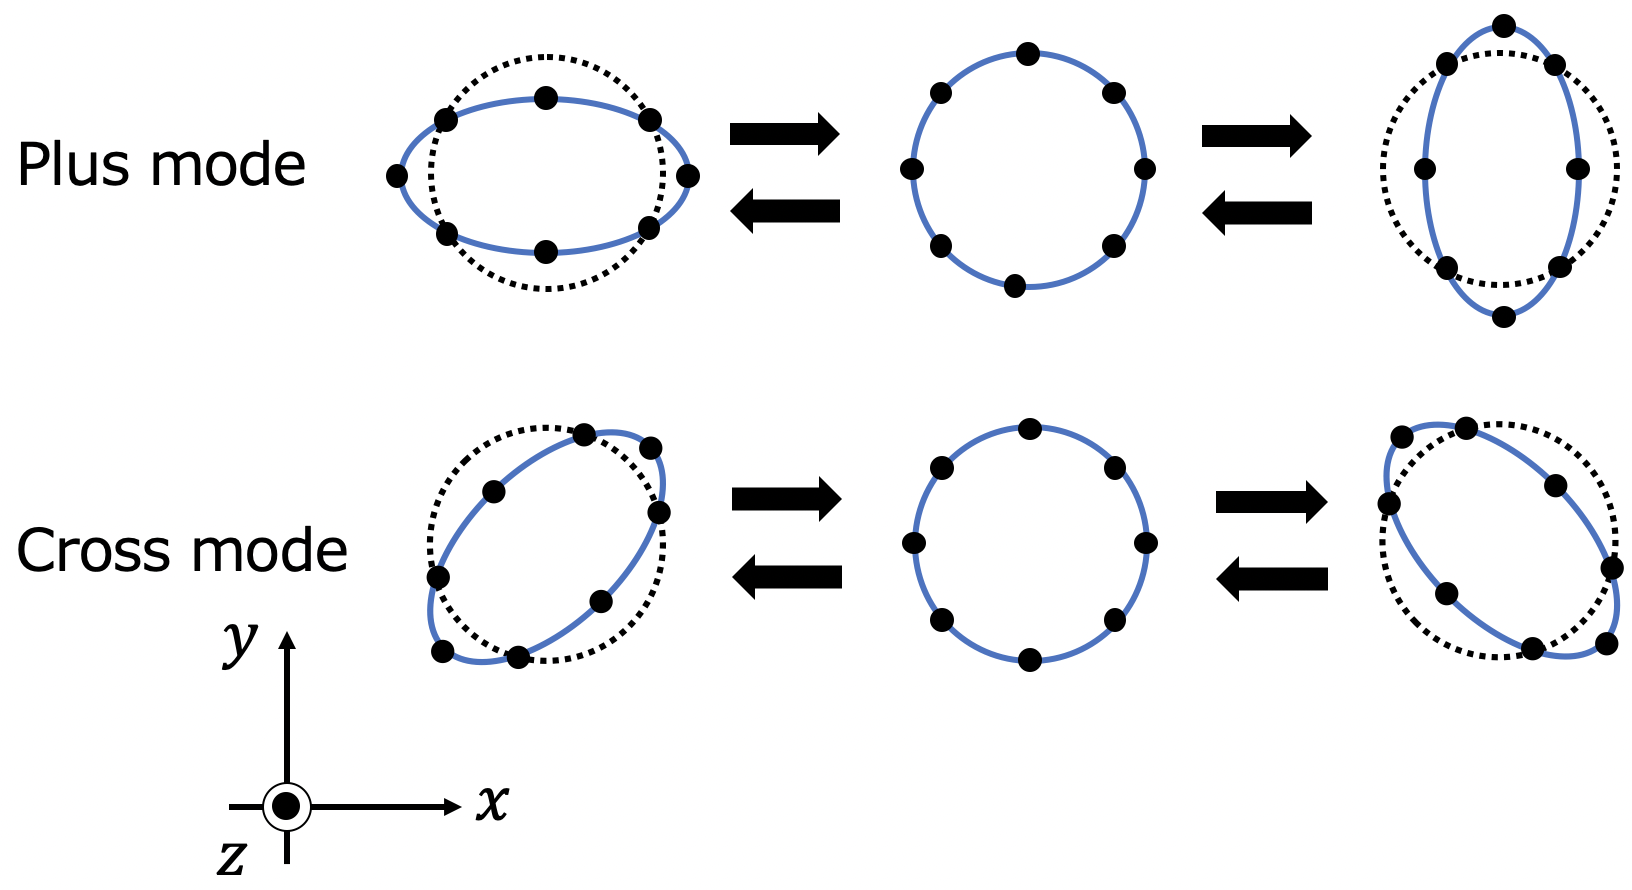
\includegraphics[width=140mm]{fig2_1.png}
\caption[重力波の偏光モード]{重力波の偏光モードの模式図. 重力波の入射によって, 質点間の固有距離が中央の初期状態から潮汐的に運動する様子を表している}
\label{fig2.1}
\end{center}
\end{figure}
\subsection{重力波の輻射}
電磁波の輻射から類推すると, 重力波は加速度をもった質量によって生まれることが分かる. しかし, 重力波では双極子放射が存在しない(質量は常に正であるから, 双極子モーメントが存在しない)ので, 4重極子モーメント(あるいはそれ以上の多重極)からの輻射を考えるという違いがある. \\
\quad エネルギー運動量テンソルが存在する場合, (\ref{eq2.18})式は
\begin{equation}
\Box\bar{h}_{\mu\nu}=\left(-\frac{1}{c^2}\frac{\partial^2}{\partial t^2}+\frac{\partial^2}{\partial x_i^2}\right)\bar{h}_{\mu\nu}=-\frac{16\pi G}{c^4}T_{\mu\nu},
\label{eq2.30}
\end{equation}
となる. また, Green関数$G(\bm{x}-\bm{x}^{\prime})$を
\begin{equation}
G(\bm{x}-\bm{x}^{\prime})=\frac{1}{4\pi\left|\bm{x}-\bm{x}^{\prime}\right|}\delta(x^0_{\rm ret}-x^{\prime0})
\end{equation}
\begin{equation}
x_{\rm ret}^0\equiv ct_{\rm ret},\quad t_{\rm ret}=t-\frac{\left|\bm{x}-\bm{x}^{\prime}\right|}{c},
\end{equation}
と書くと式(\ref{eq2.30})の解として
\begin{equation}
\bar{h}_{\mu\nu}(x^0,\bm{x})=\frac{4G}{c^4}\int\frac{T_{\mu\nu}\left(x^0-\frac{\left|\bm{x}-\bm{x}^{\prime}\right|}{c},\bm{x}^{\prime}\right)}{\bm{x}-\bm{x}^{\prime}}{\rm d}\bm{x}^{\prime},
\label{eq2.33}
\end{equation}
を得る. 真空でない($T_{\mu\nu}\neq0$)範囲が十分小さく, 観測者が波源から十分離れているとすると式(\ref{eq2.33})は多重極展開の最低次の項として, 
\begin{equation}
\bar{h}_{ij}(t,\bm{x})=\frac{1}{r}\frac{2G}{c^4}\ddot{Q}_{ij}(t^{\prime}),
\label{eq2.34}
\end{equation}
となる. ただし, $r\equiv\left|\bm{x}-\bm{x}^{\prime}\right|$,$t^{\prime}\equiv t-r/c$であり, $Q_{ij}$は四重極モーメント
\begin{equation}
Q_{ij}(t^{\prime})=\int\rho(t^{\prime},\bm{x})\left(x_{i}^{\prime}x_{j}^{\prime}-\frac{1}{3}\delta_{ij}x^{i\prime}x^{j\prime}\right)d\bm{x}^{\prime},
\end{equation}
である.  \\
\quad また, Larmorの公式から類推すると, この時の重力波の光度は
\begin{equation}
\mathcal{L}_{\rm gw}=\frac{G}{5c^5}\left<\left(\dddot{Q}_{ij}\right)^2\right>,
\label{eq2.36}
\end{equation}
となる. ここで, 系の特徴的な質量$M$, サイズ$R$, 時間スケール$T$, 速度$v$を考えると四重極モーメントの時間3階微分は
\begin{equation}
\dddot{Q}_{ij}\sim\frac{MR^2}{T^3}\sim\frac{Mv^3}{R},
\end{equation}
と近似できる. これより光度(\ref{eq2.36})のオーダーを計算すると
\begin{equation}
\mathcal{L}_{\rm GW}\sim\frac{G}{c^5}\left(\frac{M}{R}\right)^2v^6\sim3.6\times10^{59}\,\,[{\rm erg}/{\rm s}]\left(\frac{r_{\rm sch}}{R}\right)^2\left(\frac{v}{c}\right)^6,
\end{equation}
となる($r_{\rm sch}=2GM/c^2$はSchwarzschild半径). このエネルギー放射率は極めて小さく, 地球上に重力波源を作るのは難しいので天体からの放射に期待しているのである. ここで天体は普通, 自己重力に束縛されているので運動エネルギーと位置エネルギーの間に関係がある(virial定理)と仮定でき, 
\begin{equation}
Mv^2\sim\frac{GM^2}{R}.
\end{equation}
これを用いると式(\ref{eq2.36})は
\begin{equation}
\mathcal{L}_{\rm GW}\sim3.6\times10^{59}\,\,[{\rm erg}/{\rm s}]\left(\frac{r_{\rm sch}}{R}\right)^5,
\end{equation}
となる. これより, コンパクト天体(ブラックホールや中性子星など)が重力波源の候補になることが分かる. \\
さらに, 輻射された重力波の振幅を考えるために式(\ref{eq2.34})に対して
\begin{equation}
h\sim\frac{1}{r}\frac{2G}{c^4}\frac{\partial^2}{\partial t^2}(MR^2)\sim\frac{1}{r}\frac{2GMv^2}{c^4}\sim\frac{r_{\rm sch}}{r}\left(\frac{v}{c}\right)^2,
\label{eq2.41}
\end{equation}
という近似を行う. また, 重力波によるエネルギー放射効率を$\epsilon$として
\begin{equation}
\epsilon\sim\left(\frac{r_{\rm sch}}{R}\right),
\end{equation}
とパラメタ化すると式(\ref{eq2.41})は
\begin{equation}
h\sim\epsilon^{2/7}\frac{r_{\rm sch}}{2r}\sim1.5\times10^{-18}\left(\frac{\epsilon}{0.1}\right)^{2/7}\left(\frac{M}{M_{\odot}}\right)\left(\frac{r}{10\,\,[{\rm kpc}]}\right)^{-1},
\end{equation}
となる(天体までの距離$r$は銀河中心程度にスケーリングした). エネルギー効率は10$\%$程度と見積もったが, それでも重力波の振幅が小さいことが分かる.  
\subsection{主な重力波源}
測定できるほど大きな振幅を持つ重力波を人工的に生成して観測するのは難しい. 例えば, $a=10$ mの棒の両端に$M=10^3$ kgの物体を取り付けて1秒間に10回転($f=\frac{\omega}{2\pi}=$10 Hz)させるとすると, 式(\ref{eq2.41})より
\begin{equation*}
h\sim\frac{2GMa^2(2\pi f)^2}{rc^4}\sim\frac{6.52}{r}\times10^{-43}\left(\frac{M}{10^{3}\,\,{\rm kg}}\right)\left(\frac{a}{10\,\,{\rm m}}\right)^2\left(\frac{f}{10\,\,{\rm Hz}}\right)^2,
\end{equation*}
となる. 一方で重力波望遠鏡の感度は$10^{-20}\sim10^{-22}$であるから, 実験室で重力波を発生させて観測するのは不可能である. \\
\quad しかし, 宇宙には重い星が加速度運動するような天体現象がいくつか存在する. コンパクト連星合体やパルサーの自転, 超新星爆発や初期宇宙における膨脹などがその例として挙げられるが, これらによる重力波を用いて新たな天体現象や宇宙の描像の獲得を目指す重力波天文学の発展に期待がかかっている. 以下ではこのような重力波源について簡単に記す. 
\subsubsection{コンパクト連星合体(チャープ波)}
\vskip3mm
ブラックホール連星あるいは中性子星連星は重力波を放出する際, 徐々にエネルギーを失って軌道半径が小さくなっていき, 最終的に合体する. この時, 軌道半径の減少に伴って周波数と振幅が増大するチャープ波形が観測される. また, その波形と理論的な予測との比較により連星の質量・スピンといった情報を得ることができ, その合体波形から中性子星の状態方程式に制限を設けたり, 一般相対性理論を検証したりと幅広い物理への応用が可能である. \\
\quad 質量$m_1$, $m_2$の星が合体するまでの時間を$t_{\rm coal}-t$とすると放出される重力波の周波数はチャープ質量
\begin{equation}
\mathcal{M}=\frac{(m_1m_2)^{3/5}}{(m_1+m_2)^{1/5}},
\end{equation}
を用いて
\begin{equation}
f=\frac{5^{3/8}}{8\pi}\left(\frac{G\mathcal{M}}{c^3}\right)^{-5/8}(t_{\rm coal}-t)^{-3/8}\sim134\,\,[{\rm Hz}]\left(\frac{1.21M_{\odot}}{\mathcal{M}}\right)^{5/8}\left(\frac{1\,\,[{\rm s}]}{t_{\rm coal}-t}\right),
\end{equation}
と書ける. 地上のレーザー干渉計型重力波望遠鏡は100 Hz付近で感度が良いように設計されており, 特定領域の質量を持つコンパクト連星の合体は最も観測しやすい波源の1つである. 実際, 人類が初めて直接観測した重力波は, ブラックホール連星の合体によるものであり\cite{5}, その後もコンパクト連星合体による重力波イベントは数多く観測されている. 
\subsubsection{パルサー(連続波)}
\vskip3mm
パルサーとは回転する中性子星のことを指す. 式(\ref{eq2.36})から分かるように, 回転軸対称な質量分布の変化では重力波は放出されないが, パルサーが回転軸に対して完全に対称でない場合はその回転周波数で連続重力波が放射される. \\
\quad この非対称性はパルサー生成時の残留非対称性やその後の質量降着などによると考えられる. また, 非対称性の大きさは中性子星の状態方程式に依るが, その状態方程式についてはよく分かっていない. よって, パルサーからの重力波を観測することによって, 非対称性のメカニズムおよび中性子星の状態方程式を解明することが期待されている. また, これまでの観測により, 中性子星の非軸対称性を表す楕円度$\epsilon$に上限値をつけることができている(例えばCrabパルサーに対しては $\epsilon\leq10^{-4}$ )\cite{20}. 
\subsubsection{超新星爆発(バースト波)}
\vskip3mm
超新星爆発とは, 非常に重い星が一生の終わりに重力崩壊や高エネルギー反応によって引き起こす爆発のことであり, 激しい質量の移動が起こるため, 非対称性が伴う爆発の場合は重力波源になりえ, バースト的な重力波が予想されている\cite{21}. その重力波により, 電磁波では観測できない超新星内部の情報を得て, 爆発のメカニズムを解明することが期待されている. その実現には超新星爆発の信号と重力波望遠鏡における突発性ノイズを区別するために, 複数台の検出器で観測を行うことが求められる. 
\subsubsection{宇宙背景重力波}
\vskip3mm
電磁波を用いて初期宇宙を直接観測することはできない. なぜなら, 宇宙誕生後の38万年間は電子と陽子が電離したプラズマ状態であるため, 電磁波は真っ直ぐに飛べないからである. それゆえ初期宇宙を直接観測する唯一の手段が重力波となる. もし初期宇宙の背景重力波を検出することができれば宇宙論を大きく進歩させるものである. \\
\quad 例えば宇宙の平坦性や地平線問題を解決するために唱えられているインフレーション理論では, 時空の量子揺らぎにより重力波が発生すると言われている. インフレーションによって引き伸ばされたこの重力波は現在もあらゆる場所を伝播しており, 背景重力波と呼ばれている. この重力波を検出することによって, インフレーション理論の検証やその後ビッグバンが起こった時期の特定など, 宇宙論における様々な問題が解決できると見込まれている. 
\subsection{重力波観測の貢献}
重力波は非常に強い透過力を持ち, 減衰しないという点で従来の観測手段とは大きく異なる. ここではそのような重力波の観測の利用例について述べる. 
\subsubsection{マルチメッセンジャー天文学}
\vskip3mm
これまでの天文学は電磁波による観測にニュートリノや宇宙線を用いた観測が加わることで進められてきた. そして, 重力波がこれまでとはまったく異なる観測手段となることで, 新たな発見・進歩が見込まれる. さらに, 電磁波やニュートリノ, および重力波の観測を同時に行うことで単独では知り得ない情報(例えばショートガンマ線バーストの起源の確定, r過程元素合成の詳細, 超新星爆発のメカニズムなど)を得られる\cite{22}. これがマルチメッセンジャー天文学であり, その実現のために各研究機関で協力体制がとられている. \\
\quad マルチメッセンジャー天文学においては重力波信号を検出した際, 電磁波観測を行う機関に連絡し, 同じ方向の観測を行なってもらう. 反対に, 電磁波観測の結果を受け, 同時刻の重力波データを解析するということも考えられる. よって, 重力波検出には波源方向の特定精度の向上, 突発性雑音による誤検出の低減などが求められる. 
\subsubsection{重力理論}
\vskip3mm
重力波観測の結果を用いた一般相対論の検証は既に始まっている. 例えば一般相対論で予想される重力波形と観測結果のずれがどのくらいかということや, 一般相対論では重力波は光速で伝播するので重力子の質量は0とされるが, 実際の観測から重力子に質量があると言えるかということなどが検証されており, 未だ破綻は見つかっていない\cite{23}. 今後は大質量ブラックホールからの重力波を高感度で観測することで, その準固有振動成分をより詳細に解析し, 一般相対論の検証に繋げることなどが見込まれる. 例えば一般相対論を仮定すると, ブラックホールでは唯一性定理(ブラックホールが質量・電荷・スピンだけで記述できるとするもの)が成り立つ. すなわち, 準固有振動における周波数や振動パターンが質量・電荷・スピンで記述できる. よって準固有振動からの重力波を詳細に観測することにより, 一般相対論の検証が可能だと考えられる. \\
\quad 他にも自然界にある4つの力を統一するため, 一般相対論と量子論を複合した量子重力理論の完成が求められているが, 超弦理論はそのような理論として有力である. これは4つの力のうち重力だけが弱く統一的に扱いにくいことを, 重力のみが余剰次元\footnote{超弦理論では時空・空間の4次元の他に, 余剰次元(7次元)があるとし, 11次元の世界の中の膜の中に我々が存在すると考える. }にしみ出すとして説明する. これを検証する手段として重力波が挙げられている. 例えば遠くの天体から到来する重力波の一部が余剰次元にしみ出した場合, 観測される重力波の強度が小さくなるので, それにより余剰次元の存在を証明するのである. このような量子重力理論理論を用いた物理法則の統一により, 宇宙の誕生および進化が説明できると考えられる. 
\section{レーザー干渉計型重力波検出器}
重力波検出器の開発は1960年代から行われてきた. 初めは重力波によって金属製の共振体の共振振動が励起されることを利用した, 共振型といわれる装置での重力波の検出を目指していたが, この装置で検出できるのは共振体の共振周波数の重力波に限られてしまう. そこで, 現在ではより広い観測帯域を持つレーザー干渉計型の検出器が主流になっている. \\
\quad このレーザー干渉計型重力波検出器は広い周波数帯域で高感度を達成するが, 重力波信号は微小であり, さまざまな雑音が感度を制限する. この節ではレーザー干渉計型重力波検出器の基本原理や問題となる雑音, 実際に観測を行っている検出器について述べる. 
\subsection{Michelson干渉計}
\subsubsection{原理}
\vskip3mm
レーザー干渉計型重力波検出器は図\ref{fig2.2}のようなMichelson干渉計を基本構成としている. 図の左側から入射したレーザー光が光のパワーを半分づつに分ける Beam Splitter (BS) によって分けられ, 直交した腕を往復した後BSで再結合し, 干渉する. 重力波検出器の場合はBSで干渉した光が全て入射側に戻り, Signal Portに光が漏れないように腕の長さが制御されている (Dark Fringe Control) . 
\begin{figure}[H]
\begin{center}
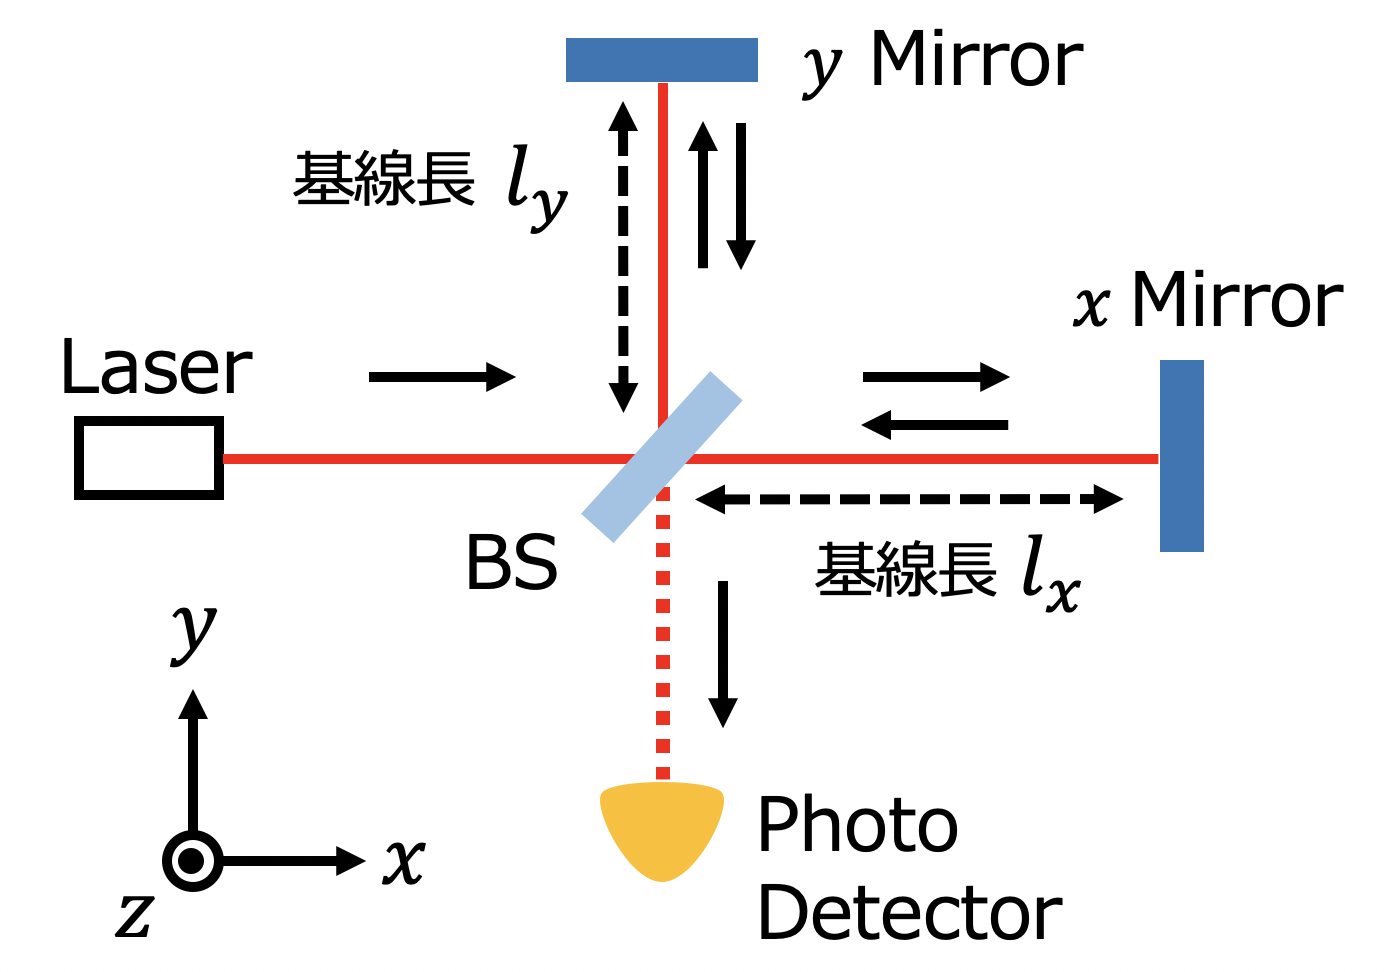
\includegraphics[width=110mm]{fig2_2.png}
\caption[Michelson干渉計]{Michelson干渉計(レーザー干渉計型重力波検出器の基本構成)の概念図}
\label{fig2.2}
\end{center}
\end{figure}
この干渉計に重力波が到来すると自由質点間(観測周波数帯域において自由質点となるよう, 鏡は振り子型の懸架装置に吊るされている)の固有距離(BSと$x,y$ Mirror間の距離)が変化し, この光路長変化によってBSに戻ってくる光に位相変調が加わる. これはキャリアである入射レーザー光に対して重力波の周波数に応じたSideband(側波帯)が生成されるということを意味している. 重力波信号を運ぶこのSidebandを信号Sidebandと呼ぶ. 信号Sidebandは二つの腕で逆位相となるので, BSでの干渉条件はレーザー光とは逆になる. つまり, 光が漏れていなかったSignal Portに信号Sidebandが抜けてくる. これを Photo Detector (PD) で検出することで, 重力波の到来が分かる. この様子を数式で示すと以下のようになる. \\
\quad レーザーから出た光を$E_0(t)=A{\rm e}^{i\Omega t}$とする(角周波数$\Omega$はレーザー光の波長$\lambda$を用いて$\Omega=2\pi c/\lambda$). BSで分かれた光は$x$ Mirrorおよび$y$ Mirrorで反射して再びBSに戻ってくる. ここで$y$ Mirrorで反射してPDに入る光が$x$ Mirrorによる反射光に対して$\delta\phi$だけ位相がずれるとするとPDで検出される光は
\begin{equation}
E_{\rm PD}(t)=E_x{\rm e}^{i\Omega t}-E_y{\rm e}^{i(\Omega t+\delta\phi)},
\end{equation}
と書ける($E_x,E_y$はそれぞれ$x,y$ Mirrorから返ってくる光の振幅). これよりPDで受け取る光の強度は
\begin{equation}
P=\left|E_{\rm PD}(t)\right|^2=\frac{P_{\rm max}+P_{\rm min}}{2}+\frac{P_{\rm max}-P_{\rm min}}{2}\cos(\delta\phi),
\end{equation}
となる. ただし, 
\begin{equation}
P_{\rm max}=\frac{(E_x+E_y)^2}{2},\,\,P_{\rm min}=\frac{(E_x-E_y)^2}{2},
\end{equation}
である. よって位相差$\delta\phi$によって強度が余弦関数的に変化することが分かる. また, $P_{\rm max}$と$P_{\rm min}$を用いて
\begin{equation}
C\equiv\frac{P_{\rm max}-P_{\rm min}}{P_{\rm max}+P_{\rm min}},
\end{equation}
が定義される. これは干渉計のコントラストと呼ばれ, 完全に干渉状態にあるとき$C=1$, 全く干渉していないとき$C=0$となる. つまり, 干渉縞の明瞭度を表す指標である. 
\subsubsection{重力波に対する応答}
\vskip3mm
さて, 重力波$h_{+}$がMichelson干渉計へ$z$方向に入射したときの応答を考える. このとき
\begin{equation}
{\rm d}s^2=-c{\rm d}t^2+(1+h_+){\rm d}x^2+(1-h_+){\rm d}y^2+{\rm d}z^2,
\end{equation}
と書ける. $x,y$ Mirrorは自由質点であるから座標は変化せず, 光は${\rm d}s^2=0$の世界線を進むので$x$軸上において
\begin{equation}
{\rm d}x=\pm\frac{c{\rm d}t}{\sqrt{1+h_{+}}}\sim\pm\left(1-\frac{1}{2}h_+\right)c{\rm d}t,
\end{equation}
である. これをBSと$x$ Mirrorの間を往復する経路(所要時間$\tau_x$)で積分すると
\begin{equation}
\frac{2l_x}{c}=\int_{t-\tau_x}^t\left(1-\frac{1}{2}h_+\right){\rm d}t^{\prime},
\end{equation}
となる. ここで重力波の振幅は極めて小さい($h\ll1$)なので積分範囲の$\tau_x$は$2l_x/c$とみなせて
\begin{equation}
\tau_x=\frac{2l_x}{c}+\frac{1}{2}\int_{t-2l_x/c}^th_+{\rm d}t^{\prime},
\end{equation}
が得られる. これより$x$軸上で1往復する際の位相変化を求めると
\begin{equation}
\phi_x=\Omega\tau_x=\frac{2l_x\Omega}{c}+\frac{\Omega}{2}\int_{t-2l_x/c}^th_+{\rm d}t^{\prime}.
\end{equation}
$y$軸上の場合も符号が異なること以外は同様に計算できるので, $l_x\sim l_y\sim l$の場合の位相差は
\begin{equation}
\delta\phi=\frac{2(l_x-l_y)\Omega}{c}+\Omega\int_{t-2l_x/c}^th_+{\rm d}t^{\prime}.
\end{equation}
この式のうち, 第2項が重力波による位相変化$\delta\phi_{\rm GW}$であり, これを読み取ることで重力波の検出が可能になる. ここで$h_+(t)$のFourier変換
\begin{equation}
h_+(t)=\int_{-\infty}^{\infty}h_+(\omega){\rm e}^{i\omega t}{\rm d}\omega,
\end{equation}
を用いると重力波による位相変化は
\begin{equation}
\delta\phi_{GW}=\int_{-\infty}^{\infty}H_{\rm MI}h_+(\omega){\rm e}^{i\omega t}{\rm d}\omega.
\end{equation}
ただし, 
\begin{equation}
H_{\rm MI}=\frac{2\Omega}{c}\sin\left(\frac{l\omega}{c}\right){\rm e}^{-\frac{i\omega l}{c}},
\label{eq2.58}
\end{equation}
である. これがMichelson干渉計の重力波に対する周波数応答になる. この式より$|H_{\rm MI}|$が最大になるのは
\begin{equation}
\frac{l\omega}{c}=\frac{\pi}{2},
\end{equation}
のときであることが分かるが, これは重力波の位相が1往復でちょうど反転する場合にMichelson干渉計の感度が最も良くなることを表している. さらに, 100 Hzの重力波を観測する場合はおよそ750 kmの腕の長さを持つ干渉計が必要であることも分かる. しかし, そのような長さの干渉計を地上に建設することは不可能であるため, 光を何度も往復させて実行的な光路長を長くするFabry-Perot型の干渉計が用いられる. 
\subsection{Fabry-Perot Michelson干渉計}
\subsubsection{Fabry-Perot共振器}
\label{sec2.2.2.1}
\begin{figure}[H]
\begin{center}
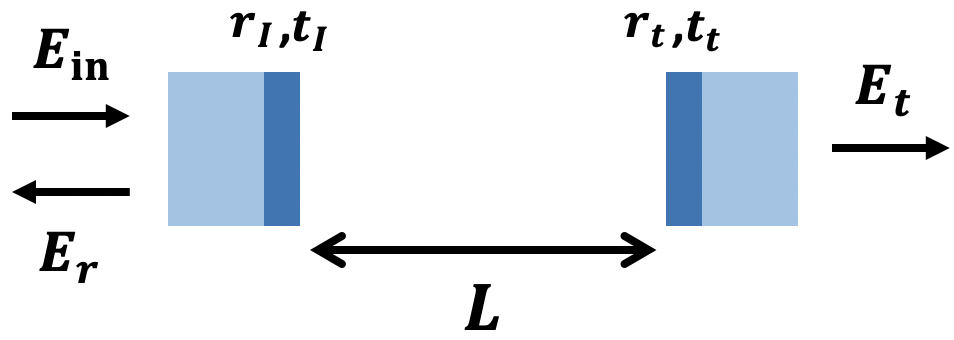
\includegraphics[width=120mm]{fig2_3.png}
\caption[Fabry-Perot Michelson共振器]{Fabry-Perot 共振器}
\label{fig2.3}
\end{center}
\end{figure}
Fabry-Perot Michelson干渉計の原理や重力波に対する応答を記す前に, Fabry-Perot共振器について概要を記す. \\
\quad 図\ref{fig2.3}のような長さ$L$のFabry-Perot共振器を考え, ITMの振幅反射率および透過率を$r_I$, $t_I$とし, ETMに対しても同様に$r_E$, $t_E$とする. このとき, 共振器の反射光電場は
\begin{equation}
E_r=-r_IE_{\rm in}+\sum\limits_{n=1}^{\infty}t_I^2r_I^{n-1}r_E^{n}{\rm e}^{i\times2nkL}E_{\rm in}=\left(-r_I+\frac{t_I^2r_E{\rm e}^{2ikL}}{1-r_Ir_E{\rm e}^{2ikL}}\right)E_{\rm in},
\end{equation}
\begin{equation}
E_t=\sum\limits_{n=1}^{\infty}t_It_Er_I^{n-1}r_E^{n-1}{\rm e}^{i\times(2n-1)kL}E_{\rm in}=\frac{t_It_E{\rm e}^{2ikL}}{1-r_Ir_E{\rm e}^{2ikL}}E_{\rm in},
\end{equation}
となる. よって共振器の振幅反射率・透過率 ($r_{cav}$, $t_{cav}$) と強度反射率・透過率 ($R_{\rm cav}$, $T_{\rm cav}$) は
\begin{align}
r_{\rm cav}&=\frac{E_r}{E_{\rm in}}=-r_I+\frac{t_I^2r_E{\rm e}^{2ikL}}{1-r_Ir_E{\rm e}^{2ikL}}\label{eq2.62}\\
t_{\rm cav}&=\frac{E_t}{E_{\rm in}}=\frac{t_It_E{\rm e}^{2ikL}}{1-r_Ir_E{\rm e}^{2ikL}}\label{eq2.63}\\
R_{\rm cav}&=\left|r_{\rm cav}\right|^2=\frac{\left[r_I-(r_I^2+t_I^2)r_E\right]^2+4r_Ir_E(r_I^2+t_I^2)\sin^2kL}{(1-r_Ir_E)^2+4r_Ir_E\sin^2kL}\label{eq2.64}\\
T_{\rm cav}&=\left|t_{\rm cav}\right|^2=\frac{(t_It_E)^2}{(1-r_Ir_E)^2+4r_Ir_E\sin^2kL},
\label{eq2.65}
\end{align}
であり, さらに入射光強度に対する共振器内の光強度は式(\ref{eq2.65})の分子において$t_E^2$で割って, 
\begin{equation}
T_{\rm cav内}=\frac{t_I^2}{(1-r_Ir_E)^2+4r_Ir_E\sin^2kL},
\label{eq2.66}
\end{equation}
と表される. なお, 鏡の反射・透過による光学的な損失がない場合は$r_I^2+t_I^2=1$であり, $R_{\rm cav}+T_{\rm cav}=1$となる. \\
\quad 式(\ref{eq2.65})において$kL=n\pi\,\,(n\in{\bm{N}})$とすると強度透過率は最大値$T_{\rm cav}^{\rm max}=\frac{(t_It_E)^2}{(1-r_Ir_E)^2}$をとり, この状態を共振状態と呼ぶ. 一方, $kL=(n+\frac{\pi}{2})$のとき, 強度透過率は最小値$T_{\rm cav}^{\rm min}=\frac{(t_It_E)^2}{(1+r_Ir_E)^2}$となり, 反共振状態と呼ばれる. \\
\quad ここで, 強度透過率をレーザー周波数の関数とみなすと, 隣り合う共振状態の周波数差は式(\ref{eq2.65})より
\begin{equation}
\nu_{\rm FSR}=\frac{c}{2L},
\end{equation}
と表され, フリースペクトラルレンジ (Free Spectral Range : FSR) と呼ばれる. また, Fabry-Perot共振器を構成する鏡の反射率が1に近い時は$T_{\rm cav(\nu)}$は$\nu_{\rm FSR}$間隔で鋭いピークを持つ(図\ref{fig2.4}). このピークの半値全幅を$\nu_{\rm FWHM}(r_I,r_E)$とすると, 
\begin{equation}
T_{\rm cav}(\nu_{\rm FWHM})=\frac{1}{2}T_{\rm cav}^{\rm max},
\end{equation}
であり, 
\begin{equation}
\nu_{\rm FWHM}(r_I,r_E)=\frac{c(1-r_Ir_E)}{2\pi L\sqrt{r_Ir_E}},
\end{equation}
と書ける. ここで$\nu_{\rm FSR}$と$\nu_{\rm FWHM}$の比をとると, 
\begin{equation}
\mathcal{F}(r_I,r_E)=\frac{\nu_{\rm FSR}}{\rm FWHM}=\frac{\pi\sqrt{r_Ir_E}}{1-r_Ir_E},
\label{eq2.70}
\end{equation}
となる. この$\mathcal{F}$はフィネスと呼ばれ, Fabry-Perot共振器の共振の鋭さを表している. 
\begin{figure}[H]
\begin{center}
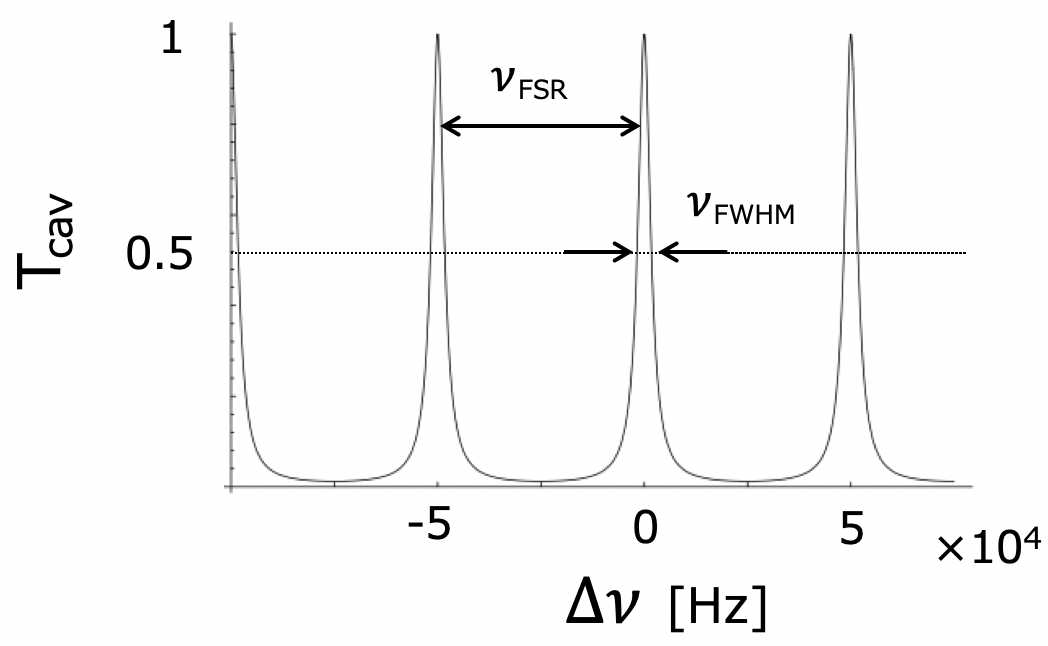
\includegraphics[width=120mm]{fig2_4.png}
\caption[Fabry-Perot共振器の強度透過率]{Fabry-Perot共振器の強度透過率. 横軸はある共振周波数からのずれである. また, 縦軸は適当な値に規格化してある. }
\label{fig2.4}
\end{center}
\end{figure}
\subsubsection{原理}
\vskip3mm
Fabry-Perot Michelson干渉計 (Fabry-Prrot Michelson Interferometer : FPMI) は図\ref{fig2.5}に示したように, Michelson干渉計のBSと各鏡の間にもう1つずつ鏡を入れた構成になっている. 各腕の2個の鏡で構成された共振器がFabry-Perot共振器であり, 向かい合う鏡間の距離を光の波長の半整数倍に調整して光を共振させている. \\
\quad FPMIではBSから入射した光は, 一部の光が透過するような薄膜コーティングが施された Input Test Mass (ITM)を透過し, ほぼすべての光が反射するような薄膜コーティングがなされた End Test Mass (ETM) で反射し, 再びITMに戻る. また, 鏡の共振器側は反射コーティングがなされているため, ETMからITMへ戻ってきた光は再度ETMへ反射される. このコーティングの反射率を調整して共振器内の光が少しずつBS側に滲み出ていくようにすることで, 光はある平均折り返し回数$n$で共振器の外へと出ていくとみなせるようになる. 
\begin{figure}[H]
\begin{center}
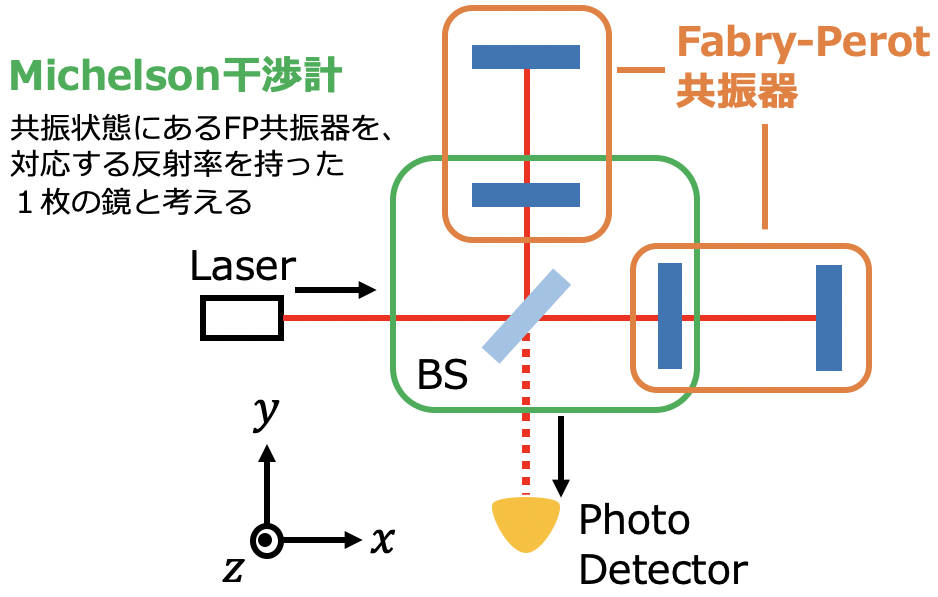
\includegraphics[width=120mm]{fig2_5.png}
\caption[Fabry-Perot Michelson干渉計]{Fabry-Perot Michelson干渉計の概念図}
\label{fig2.5}
\end{center}
\end{figure}
\subsubsection{重力波に対する応答}
\vskip3mm
先ほどと同様に, 重力波$h_{+}$がFPMIへ$z$方向に入射したときの応答を考える. 光が$\tau_n$の時間をかけて共振器を$n$回往復したとすると
\begin{equation}
\tau_n=\frac{2L}{c}n+\frac{1}{2}\int_{-\infty}^{\infty}h_+(\omega)\frac{1-{\rm e}^{-2inL\omega/c}}{i\omega}{\rm e}^{i\omega t}{\rm d}\omega,
\end{equation}
となる. ここで, ITMの反射率および透過率を$r_I,t_I$, ETMの反射率を$r_E$とし, 光が共振器長$L$だけ進んだときの位相変化を$\Delta$とするとFabry-Perot共振器内で反射される光の振幅は
\begin{equation}
E_r=E_0\left(r_I-t_I^2r_E\sum_{n=0}^{\infty}r_I^{n}r_E^{n}\right){\rm e}^{-2in\Delta},
\end{equation}
と書ける. 共振しているときは$\Delta=n\pi$なので$h$の1次まで計算すると
\begin{equation}
E_r\sim E_0\frac{r_I-r_E(t_I^2+r_I^2)}{1-r_Ir_E}\left(1-i\int_{-\infty}^{\infty}H_{\rm FP}(\omega)h_+(\omega){\rm e}^{i\omega t}{\rm d}\omega\right),
\end{equation}
となる. ただし, 
\begin{equation}
H_{\rm FP}=\frac{2\alpha\Omega}{\omega}\frac{\sin(\omega L/c)}{1-r_Ir_E{\rm e}^{-2i\omega L/c}}{\rm e}^{-i\omega L/c},
\end{equation}
\begin{equation}
\alpha=\frac{t_I^2r_E}{r_I-(r_I^2+t_I^2)r_E},
\end{equation}
である. この$H_{\rm FP}$がFPMIの周波数応答を示し, 
\begin{equation}
|H_{\rm FP}|=\frac{2\alpha\Omega}{\omega(1-r_Ir_E)}\frac{|\sin(\omega L/c)|}{\sqrt{1+F\sin^2(\omega L/c)}},
\end{equation}
となる. ここで$F$はフィネスを用いて
\begin{equation}
F=\frac{4r_Ir_E}{(1-r_Ir_E)^2}=\frac{2\mathcal{F}}{\pi},
\end{equation}
と表される値である. \\
\quad また, 光が共振器内を動く間の重力波の時間変化が十分小さい, すなわち$\omega L/c\ll 1$のときは
\begin{equation}
\begin{split}
|H_{\rm FP}|&\simeq\frac{2\alpha\Omega}{\omega(1-r_Ir_E)}\frac{\omega L/c}{\sqrt{1+F(\omega L/c)^2}}\\
&=\frac{2\alpha\Omega L}{c(1-r_Ir_E)}\frac{1}{\sqrt{1+\left(\frac{\sqrt{F}L}{c}\omega\right)^2}}\\
&=\frac{2\alpha\Omega L}{c(1-r_Ir_E)}\frac{1}{\sqrt{1+\left(\frac{\omega}{\omega_c}\right)^2}}
\end{split},
\label{eq2.78}
\end{equation}
となり, キャビティポール$2\pi\omega_c$の1次のローパス特性を保つことが分かる. ここで, 
\begin{equation}
\omega_c=\frac{c}{\sqrt{F}L}=\frac{c(1-r_Ir_E)}{2L\sqrt{r_Ir_E}},
\end{equation}
であり, 
\begin{equation}
\nu_c=\frac{\omega_c}{2\pi}=\frac{c(1-r_Ir_E)}{4\pi L\sqrt{r_Ir_E}}=\frac{1}{2}\nu_{\rm FWHM},
\end{equation}
は cut-off 周波数である. また, キャビティポールの逆数
\begin{equation}
\tau=\frac{1}{\omega_c}=\frac{2L\sqrt{r_Ir_E}}{c(1-r_Ir_E)},
\end{equation}
は光が共振器内に滞在する平均時間 (strage time) を表す. この平均滞在時間は式(\ref{eq2.70})を用いて
\begin{equation}
\tau=\frac{2L}{\pi c}\mathcal{F},
\label{eq2.82}
\end{equation}
と表せる. 一方, Fabry-Perot共振器における折り返し数を$N_{\rm FP}$とすると
\begin{equation}
\tau=N_{\rm FP}\frac{2L}{c},
\end{equation}
なので, 式(\ref{eq2.82})と合わせて
\begin{equation}
N_{\rm FP}=\frac{\mathcal{F}}{\pi},
\end{equation}
となり, 折り返し数をフィネスで表すことができる. \\
\quad 最後にMichelson干渉計の場合と比較する. 重力波に対する周波数応答の比を取ると, 式(\ref{eq2.58})と式(\ref{eq2.78})より, 
\begin{equation}
\frac{\left|H_{\rm FP}\right|}{\left|H_{\rm MI}\right|}=\frac{2\alpha}{1-r_Ir_E}\frac{1}{\sqrt{1+\left(\frac{\omega}{\omega_c}\right)^2}},
\end{equation}
となる. この式において$r_E\rightarrow 1,\omega\ll\omega_c$とすると
\begin{equation}
\frac{\left|H_{\rm FP}\right|}{\left|H_{\rm MI}\right|}\rightarrow\frac{4}{T_I},
\end{equation}
であり, この極限で FPMIは実効的にアーム長が$4/T_I$のMichelson干渉計とみなすことができる. また, 両者の周波数応答を図\ref{fig2.6}に示した. 低周波ではFPMIの腕共振器の影響により, Michelson干渉計よりも応答が増幅されるが, キャビティポール(cut-off 周波数)より高周波では信号が減衰されてしまう. 
\begin{figure}[H]
\begin{center}
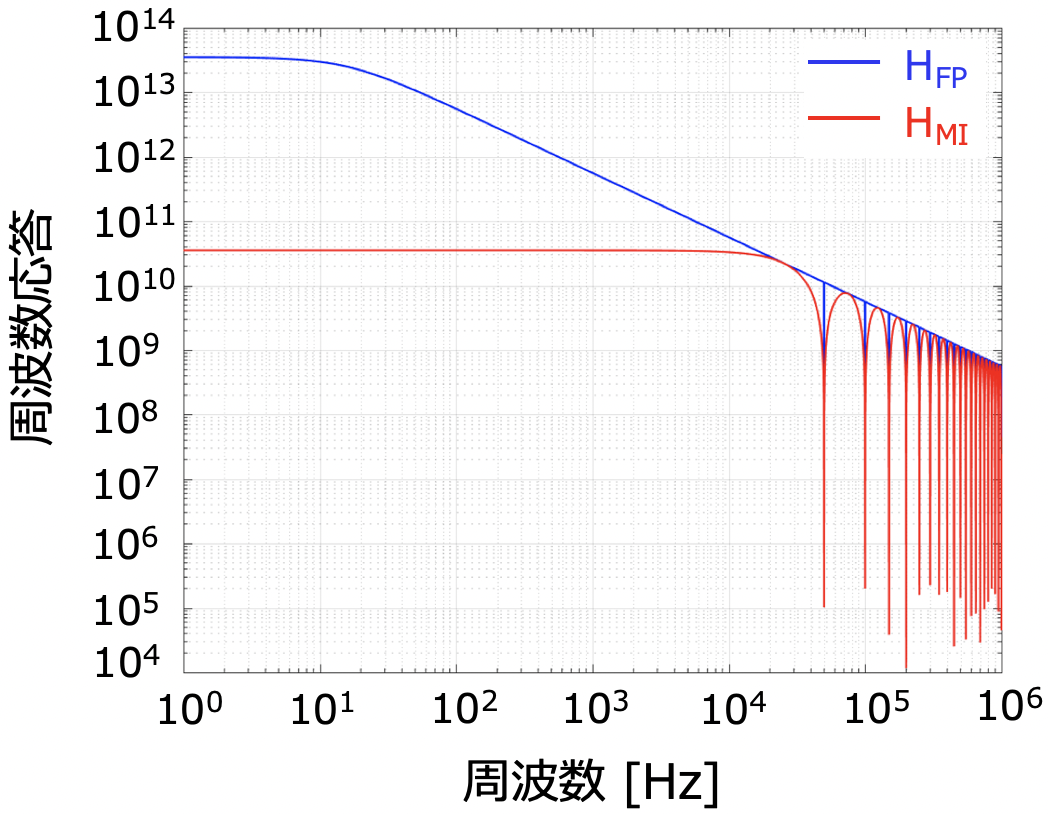
\includegraphics[width=130mm]{fig2_6.png}
\caption[Michelson干渉計とFPMIの周波数応答]{Michelson干渉計 (3 km) とFPMI (腕共振器の長さ3 km) の周波数応答. 低周波において, FPMIでは腕共振器の影響で, Michelson干渉計よりも応答が増幅される. しかし, キャビティポール(cut-off 周波数)より高周波では信号が減衰されてしまう.  }
\label{fig2.6}
\end{center}
\end{figure}
\subsection{DRFPMI}
FPMIにパワーリサイクリングとRSEを導入した干渉計を Dual-Recycled Fabry-Perot Michelson Interferimeter (DRFPMI) と呼び, 現在はこの形がレーザー干渉計型重力波検出器の主流なものとなっている. なお図\ref{fig2.7}に示したように, DRFPMIには全部で5つの長さ自由度がある. \\
\quad まず, DARMと呼ばれるのはFabry-Perot共振器の差動変動であり, 重力波信号はこの自由度の変動として現れる. 一方CARMはFabry-Perot共振器長の同相成分である. CARMの信号は共振器長変動の同相成分であり, レーザーの周波数揺らぎを反映するようになっているので, この自由度を用いてレーザー周波数の安定化を行う. また, PRCLおよびSRCLはPower Recycling Cavity (PRC), Signal Recycling Cavity (SRC) の長さであり, それぞれ2枚のITMとPower Recycling Mirror (PRM), Signal Recycling Mirror (SRM) の距離の平均で表される. 最後に, MICHとはMichelson干渉計部分の自由度である. 以下ではパワーリサイクリングとRSEについて簡単に記す. 
\begin{figure}[H]
\begin{center}
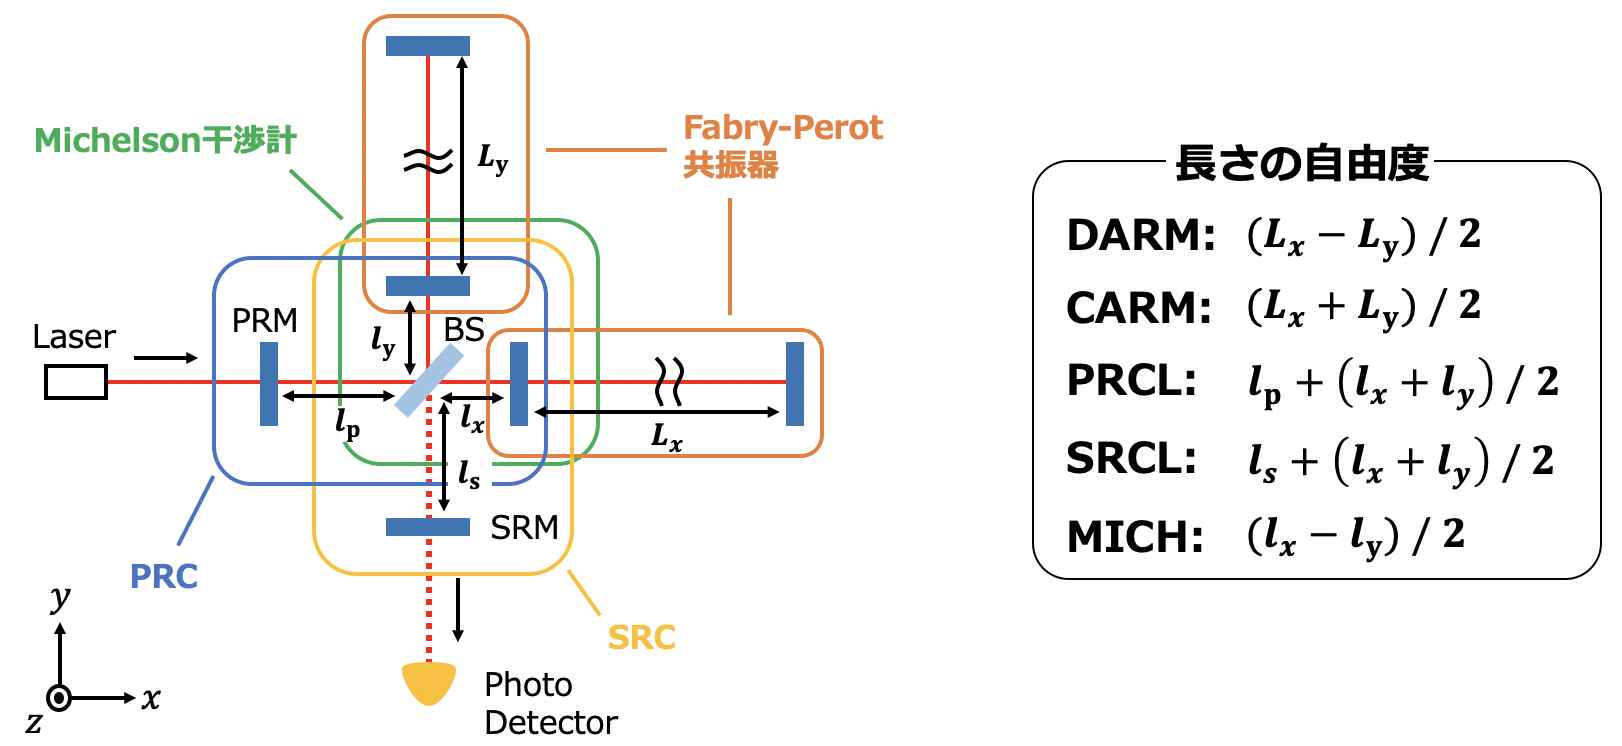
\includegraphics[width=170mm]{fig2_7.png}
\caption[DRFPMI干渉計]{DRFPMI干渉計の概念図および長さの自由度}
\label{fig2.7}
\end{center}
\end{figure}
\subsubsection{パワーリサイクリング}
\vskip3mm
重力波検出器では, 散射雑音の最小化のため, 干渉計のSignal Portから光が漏れないような制御をしている. そのため, レーザーパワーのほとんどが入射側へと戻っていく. 一方, 重力波信号を大きくするためには重力波と相互作用する腕共振器内のレーザーパワーを上げる必要がある. そこで, 戻っていくレーザーをFPMIに打ち返す鏡を入射側に置き, 実効的なレーザーパワーを増大させている. これにより, 散射雑音レベルを改善することができる\cite{power}. \\
\quad この手法をパワーリサイクリングと呼び, 打ち返しを行う鏡を Power Recycling Mirror (PRM) と呼ぶ(図\ref{fig2.7}). このとき, 入射側から見たFPMIは全体として1つの鏡とみなすことができる(レーザーをPRM側に反射している). ここで, 光共振器において, 二つの鏡の反射率が等しい場合, 入射したレーザーパワーは内部で熱に変わるか, あるいは透過する. しかし, 重力波検出器ではETMの反射率が極めて高いので, ほとんどの光は熱に変換されるまでの間, 干渉計内にとどまる. よって, FPMIを1つの鏡とみなしたときの反射率とPRMの反射率を一致させることで, 入射レーザーパワーを最大効率で利用できるのである. \\
\quad また, 2つのITMとPRMで構成される共振器は Power Recycling Cavity (PRC) と呼ばれる. このPRCはPRMと腕共振器の複合鏡からなる共振器とみなせる. そこで, 式(\ref{eq2.66})において$r_I\rightarrow r_P$, $t_I\rightarrow t_P$, $r_E\rightarrow r_{\rm Acav}$, $L\rightarrow l_p$と置き換えると, 入射光電場$E_{\rm in}$に対する, BSでの光電場$E_{\rm BS}$の強度増幅率$G_P$が得られる. なお, $r_p$, $t_p$はPRMの振幅反射率および振幅透過率, $r_{\rm Acav}$は腕共振器の振幅反射率である. パワーリサイクリングでは, 光電場がPRC長$l_{P}$に対して共振状態となるようにするので
\begin{equation}
G_P=\frac{t_P^2}{\left(1-r_Pr_{\rm Acav}\right)^2},
\end{equation}
となる. ここで, 共振器の振幅反射率を表した式(\ref{eq2.62})において, 共振状態を考えるとPRCに対して
\begin{equation}
r_{\rm PRC}=\frac{-r_P+\left(r_P^2+t_P^2\right)r_{\rm Acav}}{1-r_Pr_{\rm Acav}},
\end{equation}
である. 光学損失がないとすると, $r_P=r_{\rm Acav}$のときに$r_{\rm PRC}=0$となるのでこれが最適条件であり, このとき$G_P$は
\begin{equation}
G_P=\frac{1}{t_P^2}=\frac{1}{T_P},
\end{equation}
となり, PRMの強度透過率に反比例する. なお, $G_P$はパワーリサイクルゲインと呼ばれ, KAGRAではこの値は10となっている. 
\subsubsection{Resonant Sideband Extraction}
\vskip3mm
Fabry-Perot共振器のフィネスを上げることで光子の折り返し数が増え, 重力波信号が増幅されるが, 1つの光子が共振器内に留まっている間に重力波の符号が反転してしまう. これにより光子に蓄積された位相変化がキャンセルされ, 高周波で重力波信号に対する感度が落ちてしまう. そこで Resonant Sideband Extraction (RSE) と呼ばれる手法を用いる\cite{RSE}. \\
\quad RSEでは Signal Recycling Mirror (SRM) がSignal Port側に置かれる(図\ref{fig2.7}). この鏡とFabry-Perot共振器のITM2枚で Signal Recycling Cavity (SRC) を構成しており, 重力波が入射したときに生成される信号SidebandがSRCに共振するようにSRCの長さを制御している. このとき, 信号SidebandにとってのSRCの反射率(Fabry-Perot共振器内から見たITMの反射率)はITM単体よりも低くなる. よって信号Sidebandに対するFabry-Perot共振器の実効的なフィネスが下がる, すなわち信号SidebandだけFabry-Perot共振器内の滞在時間が減り, 高周波での信号減衰の程度が小さくなる. なお, レーザー光にとってはFabry-Perot共振器のフィネスは高いままなので, 重力波信号の増幅率は変わらない. \\
\quad また, SRCはキャリアに対して共振もしくは反共振に制御するかの違いで, それぞれBroad Resonant Sideband Extraction (BRSE), Broadband Signal Recycling (BSR) と呼ばれる(図\ref{fig2.8}). \\
\quad BRSEではSRMとITMの複合鏡の振幅反射率が小さくなり, 腕共振器でのキャリアの平均往復回数が小さくなるため, 低周波において信号増幅率が低下する. 一方, 高周波では信号が相殺する前に腕共振器から抜き出すことで, 信号を増幅している(signal extraction). BSRではその全く逆で, 低周波では信号増幅率が高く (signal recycling), 高周波では信号相殺の影響が大きくなる. これをまとめると, BRSEとBSRの周波数応答は図\ref{fig2.9}のようになる. 
\begin{figure}[H]
\begin{center}
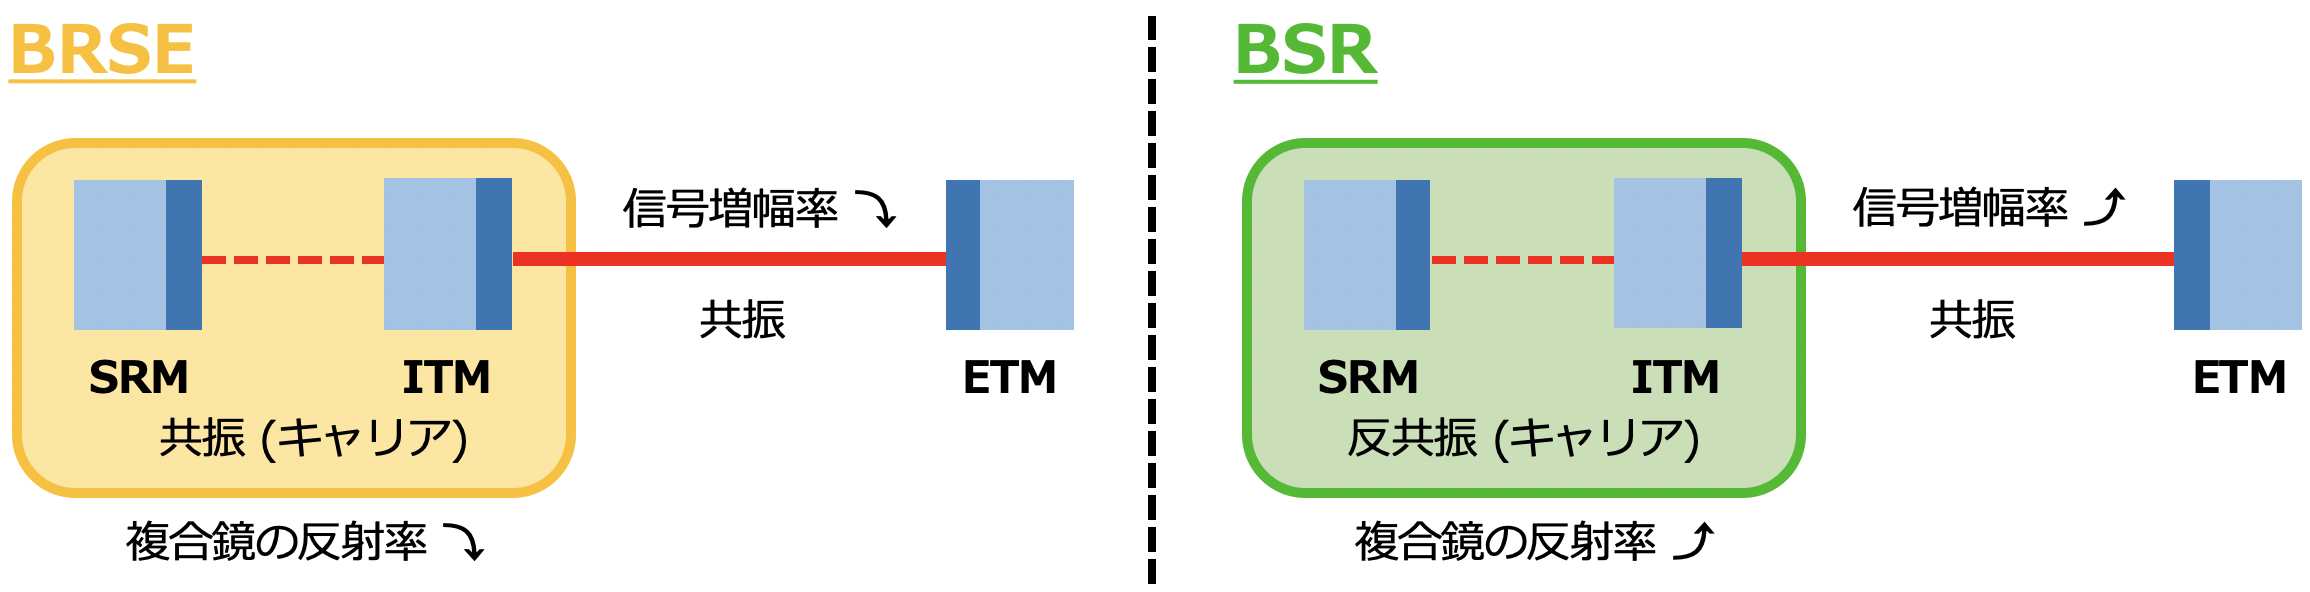
\includegraphics[width=170mm]{fig2_8.png}
\caption[SRCのモード]{SRCのモード. BRSEではSRMとITMの複合鏡の振幅反射率が小さくなり, 腕共振器でのキャリアの平均往復回数が小さくなるため, 低周波において信号増幅率が低下する. 一方で, 高周波では信号が増幅される. BSRではその逆となる. }
\label{fig2.8}
\end{center}
\end{figure}
\begin{figure}[H]
\begin{center}
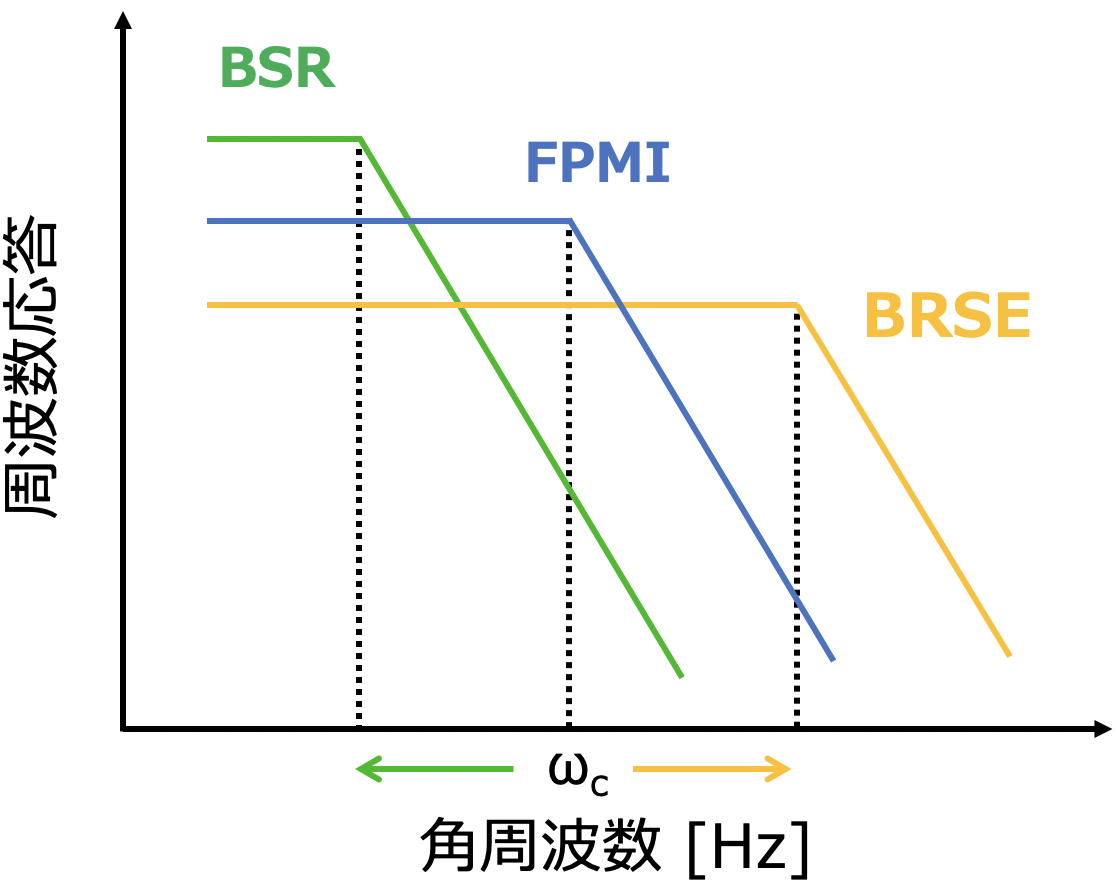
\includegraphics[width=110mm]{fig2_9.png}
\caption[光の散射雑音スペクトルの概念図]{重力波に対する周波数応答の比較. BRSEではFPMIに比べ, 低周波において信号増幅率が低下する一方で, 高周波において信号相殺の影響が小さくなる. BSRではその逆となる. }
\label{fig2.9}
\end{center}
\end{figure}
\subsection{レーザー干渉計型重力波検出器の雑音源}
重力波による長さ変動は小さく, 重力波検出器は種々の雑音に感度を制限される(図\ref{fig2.10}). ここでは干渉計の感度を決める基本的な雑音源をまとめる. 
\begin{figure}[H]
\begin{center}
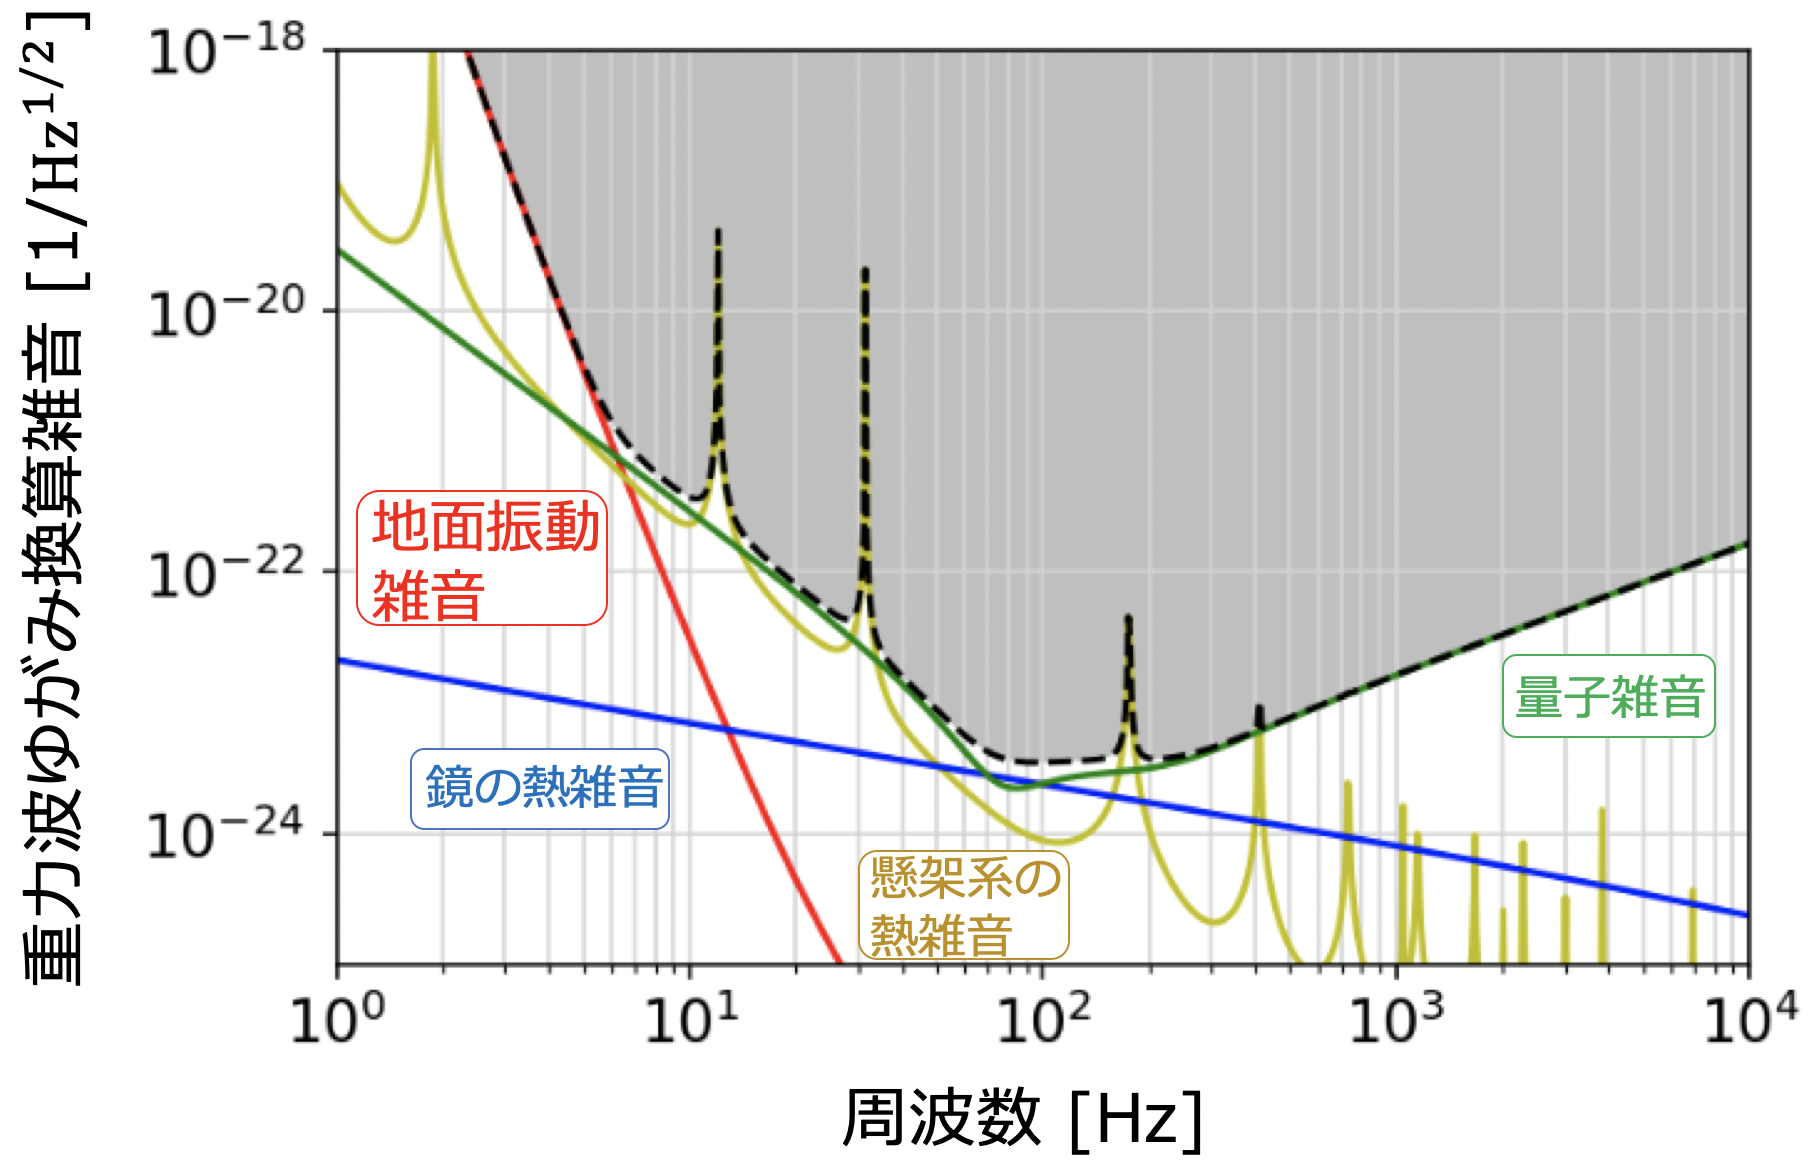
\includegraphics[width=140mm]{fig2_10.png}
\caption[KAGRAの感度曲線]{KAGRAの感度曲線. 10 Hz以下の低周波では主に地面振動や懸架系の熱雑音によって感度が制限される. また, 量子雑音は広い帯域で感度を制限している. }
\label{fig2.10}
\end{center}
\end{figure}
\subsubsection{量子雑音}
\vskip3mm
干渉計による重力波検出には, レーザー出力に起因する量子雑音がある. 量子非破壊測定を行わない場合, 量子雑音は光の位相の量子的揺らぎに起因する散射雑音と振幅の揺らぎに起因する輻射圧雑音に分けられる. \\
\quad 散射雑音は, レーザービーム中の光子数の量子的な揺らぎによって生じるノイズである. 検出器の出力に現れる重力波の信号は干渉計への入射パワー$P_0$に比例し(\ref{sec2.2.2.1}節), PDでの光子数の量子揺らぎは$\sqrt{P_0}$に比例する. よって, 重力は信号へと換算した散射雑音は$1/\sqrt{P_0}$に比例する. これより, 干渉計に入射するレーザーのパワーを上げることで散射雑音を低減することができる. なお, 散射雑音は約100 Hz以上の高周波帯で感度を制限している\cite{LIGO}. \\
\quad 一方, 輻射圧雑音は鏡の表面に作用する輻射圧の揺らぎによって発生するノイズである. このとき, 鏡に加わる力の量子揺らぎは$\sqrt{P_0}$に比例するため, 輻射圧雑音は$\sqrt{P_0}/m$に比例する. よって, 鏡の質量を大きくするか, 入射レーザーパワーを下げることで輻射圧雑音を改善することができる. なお, 輻射圧雑音は数10 Hz帯で感度を制限している\cite{LIGO}. \\
\quad これより, 散射雑音と輻射圧雑音は量子揺らぎはレーザーパワーに対して反対の依存性を持つため, 干渉計の感度への寄与はトレードオフの関係となる. また, この関係から導かれる量子雑音の下限は標準量子限界 (SQL) と呼ばれている. このSQLを超えるためには, 周波数依存性スクイージングやホモダイン検波によって量子雑音(特に輻射圧雑音)を低減するなどの方法がある\cite{24}. 
\subsubsection{熱雑音}
\vskip3mm
有限温度での原子の熱振動は鏡の表面軸位置や弾性形状の変動を引き起こし, 干渉計の光路長変動に関わる. この雑音を一般に熱雑音と呼ぶ. \\
\quad 重力波望遠鏡における熱雑音にもさまざまなものがある. 例えば熱浴とのやり取りによって懸架ファイバーの物理的振動が励起される\cite{25}. これについて, 有限温度$T$の熱浴に接した物体では, $k_BT$のエネルギーがその物体の各振動モードに分配され, 機械的な振動を行う. このとき熱振動のパワースペクトルは揺動散逸定理\cite{26}より, 
\begin{equation}
S_x(f)=-\frac{4k_BT}{2\pi f}{\rm Im}[H(2\pi f)],
\end{equation}
と表される. ただし, $k_B$はBoltzmann定数, $T$は刑が接する熱浴の温度, $H$は系が受ける外力から変位への伝達関数, $f$は周波数である. これより, 例えば
\begin{equation}
H(2\pi f)=\frac{1}{m(2\pi)^2\left[f_0^2(1+i\phi(f))-f^2\right]},
\end{equation}
という伝達関数で表された振動子の熱振動のパワースペクトルは
\begin{equation}
S_x(f)=-\frac{4k_BT}{m(2\pi)^3f}\frac{f_0^2\phi(f)}{(f^2-f_0^2)^2+f_0^4\phi^2(f)},
\end{equation}
となる. ここで, $\phi(f)$は散逸と呼ばれ, 振動子のエネルギー損失を特徴付ける量である. また, 散逸にはviscous damping(系の速度に比例した抵抗力が働くモデル)とstructure damping(材質に固有の構造減衰モデル)の2種類のモデルがあり, それぞれの場合で
\begin{equation}
\phi_v(\omega)=\frac{\omega}{\omega_0Q},
\end{equation}
\begin{equation}
\phi_s(\omega)=\frac{1}{Q},
\end{equation}
と表される. ただし, Qは共振の鋭さを表すパラメータであり, この値が大きいほど振動のエネルギーはピークに押し込められる. \\
\quad また, 懸架した鏡に入射するレーザーによる熱は, 懸架ファイバーを通して懸架系の上段へ伝えられる. そして, その熱はいくつかのステージを経由して冷却器へ流れる. このとき懸架ファイバーには下段から上段にかけて温度勾配が形成されるが, その温度勾配が緩和される際に変形を生じる. これは熱弾性雑音 (thermoelastic noise) と呼ばれている\cite{27}. \\
\quad 熱雑音を低減するためには鏡や懸架系の部品に機械的損失の小さな材料を選択する必要がある. 重力波望遠鏡の中には室温での機械的損失が小さい, すなわち機械的Q値が高い(約$10^7$)という理由で, 鏡の基材や懸架系ファイバーの材料として石英を採用しているものがある\cite{LIGO}. さらに, 温度を下げるという方法も考えられ, KAGRAではこの方法を採用している. 極低温環境下において, 溶融石英は優れた性能を示さないため, 極低温でも高い機械的Q値を示すサファイアが鏡基材として採用されている\cite{KAGRA}. \\
\quad なお, 鏡の基材やコーティング層の機械的損失や熱伝導率, 熱膨張率などの物性的性質に起因するものを鏡の熱雑音, 懸架系のワイヤ由来のものを懸架系の熱雑音と呼んでいる (図\ref{fig2.10}). \\
\subsubsection{地面振動雑音}
\vskip3mm
地球上に建設された重力波検出器にとって, 地面振動による雑音は避けられないものである. 地面は地震がない場合でもあらゆる周波数で微小振動しており, その連続的かつ不規則な地盤の運動は常に鏡を揺らす. その結果, 光共振器の長さが変動する. 
\begin{figure}[H]
\begin{center}
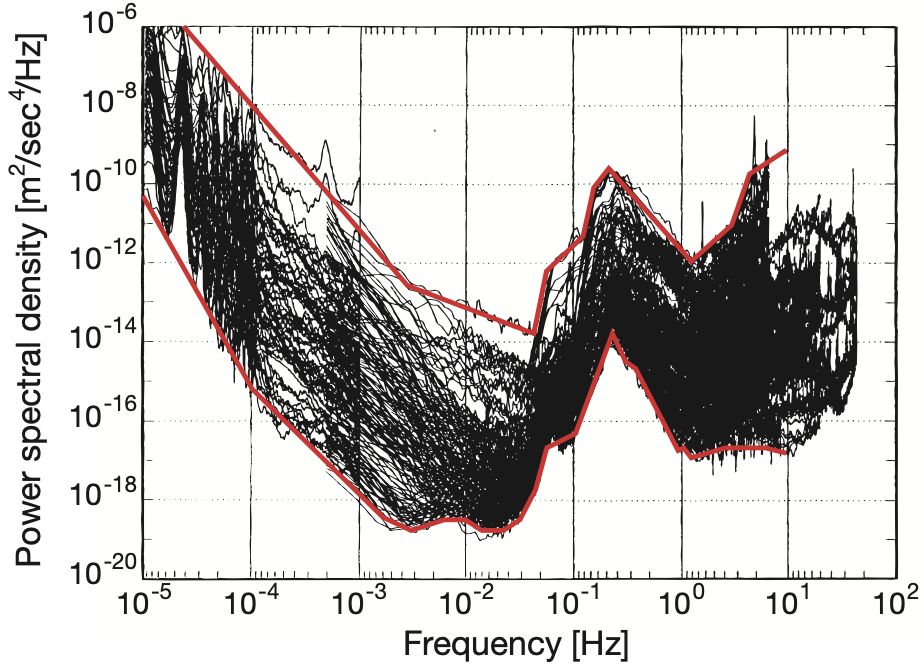
\includegraphics[width=100mm]{fig2_11.png}
\caption[NHNM/NLNMと世界中の地面振動のスペクトル]{NHNM/NLNM(赤い線がそれらを示す)と世界中の地面振動のスペクトル\cite{33}}
\label{fig2.11}
\end{center}
\end{figure}
地面振動雑音の性質は, J. Petersonによって研究されている\cite{33}. 彼は世界中の地震計のネットワークから得られた地面振動雑音スペクトルのカタログを作成した. このデータからNHNM/NLNM (New High/Low Noise Model) と呼ばれる地面振動スペクトルのモデルが構築され, 地面振動の上限と下限を与えている(図\ref{fig2.11}). 
これを見ると1 mHz以下の低周波では地面振動のスペクトルが急激に大きくなっていることがわかる(これは地球の潮汐変動による). しかし, このような低周波の地面振動では検出器のテストマスも共に移動するため, 重力波の観測を妨げることはない. 一方, 0.1$\sim$1 Hz付近にあるピークは海の波が海岸にぶつかることで発生するが, これは検出器にとって安定的な観測運転を妨げる外乱となる. また, 10 Hz以上は検出器の感度が良いため特に関心のある周波数帯である. このような地面振動の影響を低減するためには先に述べたように次の2つの点に注意する必要がある. \\
\quad a)\underline{検出器を静かな場所に建設する}\\
\qquad 図\ref{fig2.12}に示した通り, 地下 (KAGRA site) は地上 (Virgo/TAMA site) に比べて地面振動レベル\\\qquad が1桁から2桁低い. つまり, 地面振動雑音を低減するという観点から見ると, 地下に検出器を建設\\\qquad するのが良いと言える. 
\begin{figure}[H]
\begin{center}
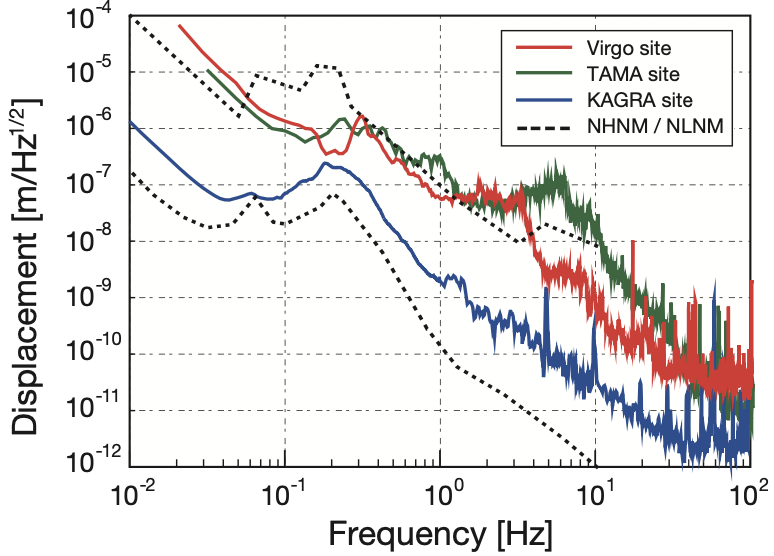
\includegraphics[width=100mm]{fig2_12.png}
\caption[地面振動雑音のスペクトル]{重力波検出器が設置されている場所での地面振動雑音のスペクトル\cite{34}}
\label{fig2.12}
\end{center}
\end{figure}
\noindent
\quad b)\underline{防振系により地面振動を減衰させる}\\
\qquad 防振系によって地面振動を減衰し, 鏡の支点に伝わる振動を小さくする必要がある. \\\qquad 防振系による地面振動の低減については第\ref{第3章}章に詳記する. 

\subsection{世界のレーザー干渉計型重力波検出器}
アメリカのinitial LIGO, イタリア・フランスのVirgo, ドイツのGEO600, 日本のTAMA300といった第1世代重力波検出器と呼ばれる検出器では, FPMIにパワーリサイクリングを組み合わせたものが主流であった. 現在はそれらの検出器に改良を加え, RSEや真空場のスクイージングなどの技術を組み込んだ第2世代重力波検出器が運用されている. また, 更なる感度向上を目指して, 第3世代の重力波検出器を地球上に建設することが計画されている. \\
\quad 以下では世界で用いられている, あるいは計画されている重力波検出器について述べる. 
\subsubsection{現在運用されている重力波検出器}
\vskip3mm
\noindent
\underline{\bm{{\large Advanced LIGO}}}\\
\quad LIGOはアメリカ(リビングストンおよびハンフォード)にある基線長4 kmのレーザー干渉計型重力波検出器である\cite{LIGO}. 2つの観測所は約3000 km離れているため, この2地点における重力波波形の相異性や到達時間の差などから, 重力波信号の真偽の判定が, ある程度できるように考慮されている. . 1990年代から重力波検出の研究を牽引してきたLIGOは, 感度向上を目指してRSEや125 Wのハイパワーレーザー, 4段の鏡懸架系などの技術を導入した後, Advanced LIGOとして観測を開始し, 2015年9月14日, 世界で初めて重力波を検出した. その後も感度向上を目指した改修作業を続け, 数多くの重力波イベントを観測している. \\\\
\underline{\bm{{\large Advanced Virgo}}}\\
\quad Virgoはイタリア(ピサ)にある基線長3 kmのレーザー干渉計型重力波検出器である\cite{Virgo}. 当初からアウトプットモードクリーナーやSuper Attenuator\cite{Virgo}と呼ばれる多段懸架系を導入していたVirgoでも, LIGOと同様の改良が行われた. そして2017年8月, Advanced VirgoとしてLIGOと共に史上4例目となる重力波検出を達成した. \\\\
\underline{\bm{{\large GEO600}}}\\
\quad ドイツ(ハノーヴァ)にある基線長600 mのレーザー干渉計型重力波検出器である\cite{GEO}. GEO600には腕共振器はないが, マイケルソン干渉計にパワーリサイクリング・シグナルリサイクリングを併用しており, 特定の周波数帯域で高感度を実現した. その後, Advanced LIGOなどとの高周波での相関検出を目指して改修され, 現在は1 kHz以上での周波数で感度を高めている. \\\\
\underline{\bm{{\large KAGRA}}}\\
\quad 日本(岐阜県飛騨市神岡町)にある基線長3 kmのレーザー干渉計型重力波検出器である\cite{KAGRA}. KAGRAでは熱雑音低減のためサファイア製の鏡を20 Kまで冷やし, かつ地面振動の影響を減らすために地下環境で運用するという特徴を持つ. 地面振動については第3章, KAGRAの干渉計のレイアウトや懸架系および冷却システムについては第3, 4章を参照されたい. 
\subsubsection{計画中の重力波検出器}
\vskip3mm
\noindent
\underline{\bm{{\large LIGO-India}}}\\
\quad LIGO-IndiaはAdvanced LIGOの部品を一式インドに送り, アメリカとインドの共同でAdvanced LIGOに相当する重力波検出器をインドに建設しようという計画である. LIGO-Indiaの完成により6台の干渉計による国際ネットワークが構築され, 波源の位置特定精度の更なる向上などが見込まれる.\\\\
\underline{\bm{{\large Cosmic ExplolerとEinstein Telescope}}}\\
\quad Cosmic ExplolerとEinstein Telescopeはどちらも将来建設が予定されている第3世代の地上重力波検出器である. Cosmic ExplolerではL字型で1辺40 kmの基線長\cite{31}, Einstein Telescopeでは1辺10 kmの正三角形にすることが予定されている\cite{32}. また, 腕の長さを伸ばしたり, 低吸収のコーティングや周波数依存スクイージングなどの技術を活用することも計画されている. 特に, 低温かつ地下環境での運転が予定されているETでは, KAGRAで培われた運用技術が応用可能であることが期待される. \\
\quad これらの新しい検出器は感度を今よりも10倍以上改善することを目指している. ここで, 重力波検出器の感度は検出可能な波源までの距離に反比例する. つまり感度が10倍良くなれば, 10倍の距離, 検出頻度(体積)で言うと1000倍に膨れ上がることになる. \\
\quad 次世代の検出器ではこのような大幅な感度向上によって, 現在の検出器では叶わないサイエンス(例えば2.1.4.2で述べたパルサーの軸対称からのずれは非常に小さく, 現在運転中の重力波検出器ではパルサーからの重力波を捉えることはできない可能性がある. 他にも, あらゆる天体に対して物理学的なモデルを確定させるためには様々な質量・スピンを持った相当数の重力波信号が必要であることを考えると, 現在の検出器では検出数が不十分である恐れがある. )を達成するという目的がある. 

\newpage
 
\newpage
\chapter{懸架系による防振}
\label{第3章}
\fontsize{11pt}{16pt}\selectfont
地上の重力波検出器の鏡は地面振動による外乱の影響を常に受けている. そのため, 防振技術が必要不可欠になる. 地面振動による鏡の揺れを低減するためには, 地面振動が元々静かな場所に検出器を建設し, さらに防振系により振動を減衰させるという方法が考えられる. \\
\quad この章では, 重力波検出器における防振の基本的な考え方について述べる. まず地多段振り子による防振について記述し, その後KAGRAの防振系について紹介する. 

\section{受動防振}
\label{sec3.1}
第2章で述べたように, レーザー干渉計型重力波検出器では重力波の到来による自由質点の固有距離の変化を測定する. しかし, 地球上では重力場の存在により自由質点を作ることが不可能である. そこで, 干渉計を構成する鏡やBSを振り子を用いて懸架することで, 共振周波数より十分高い周波数で自由質点とみなしている. \\
\quad 同時に, この振り子は地面振動からの防振を実現する役割を持つ. 以下では振り子を用いた防振システムについて説明する. 
\subsection{単振り子}
受動防振はワイヤで吊られた質点からなる単振り子でモデル化することができる. 図\ref{fig3.1}の左に示すように, 質点の質量を$m$, ワイヤ長を$l$, ワイヤの張力を$T$, 質点と地面の変位をそれぞれ$x(t),x_0(t)$で表すと, この系の運動方程式は
\begin{equation}
\begin{split}
&鉛直方向:0=T_y-mg=T\times\frac{\sqrt{l^2-(x(t)-x_0(t))^2}}{l}-mg\\
&水平方向:m\ddot{x}(t)=-T_x=-T\times\frac{x(t)-x_0(t)}{l}
\end{split}.
\end{equation}
\begin{figure}[H]
\begin{center}
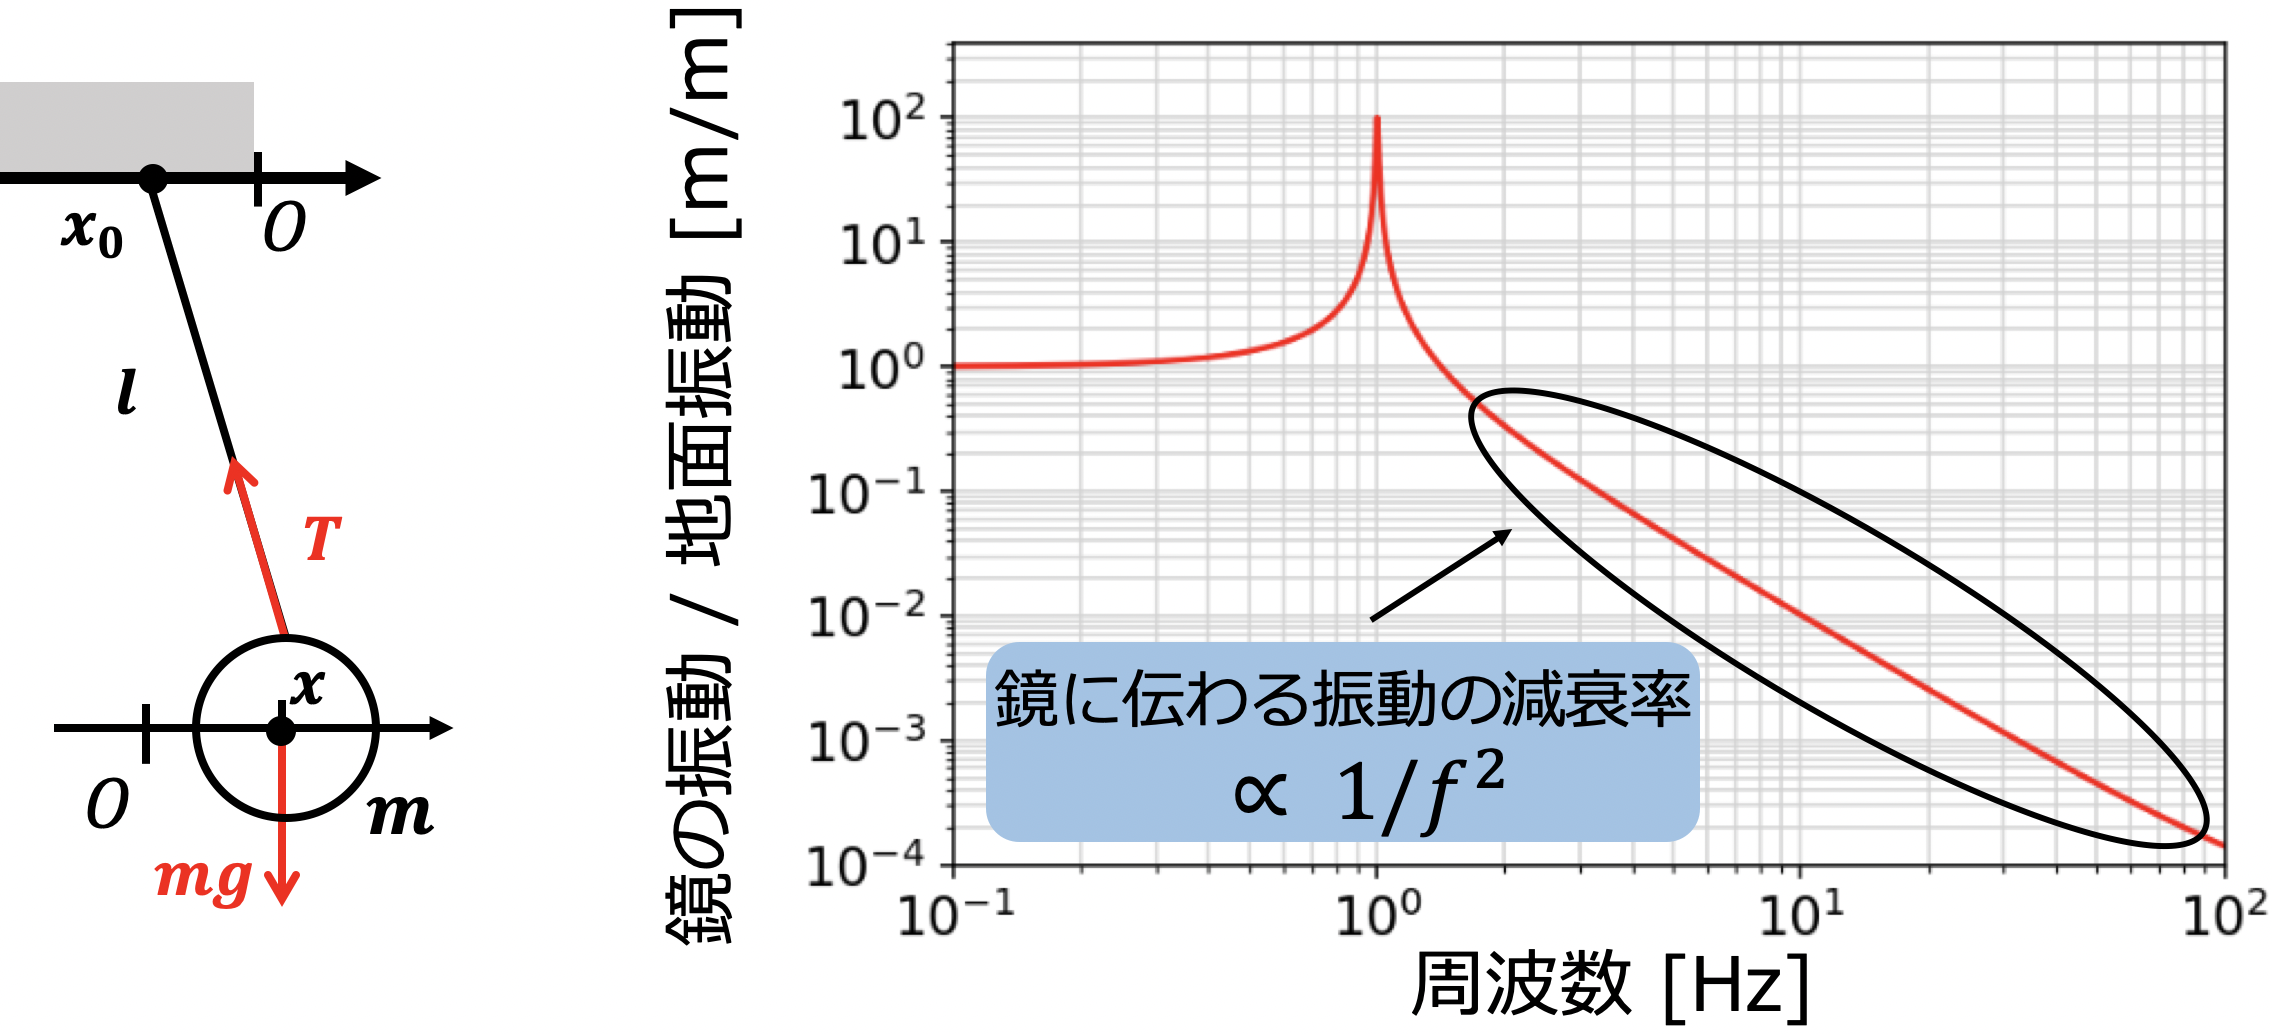
\includegraphics[width=150mm]{fig3_1.png}
\caption[単振り子による受動防振のモデルと地面振動に対する防振比]{単振り子(ワイヤーで吊られた質点)による受動防振のモデル(左)と, 地面振動に対する防振比(右). 共振周波数よりも高い周波数において, 地面から鏡に伝わる振動が周波数の2乗で減衰している. つまり, 共振周波数以上の周波数での地面振動の影響が大きく低減されている. }
\label{fig3.1}
\end{center}
\end{figure}
ここで, 水平方向の変位 $x(t)-x_0(t)$ はワイヤ長に比べて十分小さいとすると, 
\begin{equation}
\frac{\sqrt{l^2-(x(t)-x_0(t))^2}}{l}=\sqrt{1-\left(\frac{x(t)-x_0(t)}{l}\right)^2}\simeq 1,
\end{equation}
であるから, 鉛直方向の運動方程式は
\begin{equation}
0=T-mg,
\end{equation}
となる. これを水平方向の運動方程式に代入すると, 
\begin{equation}
m\ddot{x}(t)+\frac{mg}{l}(x(t)-x_0(t))=0.
\end{equation}
両辺をFourier変換すると
\begin{equation}
-m\omega^2\tilde{x}(\omega)+\frac{mg}{l}\left(\tilde{x}(\omega)-\tilde{x}_0(\omega)\right)=0.
\end{equation}
よって防振比は
\begin{equation}
\frac{\tilde{x}(\omega)}{\tilde{x}_0(\omega)}=\frac{mg/l}{-m\omega^2+mg/l}=\frac{\omega_0^2}{\omega_0^2-\omega^2}.
\end{equation}
ここで, $\omega_0$は共振角周波数で, $\omega_0\equiv2\pi f_0=\sqrt{g/l}$である. \\
\quad この防振比を表したものが図\ref{fig3.1}の右側である. これを見ると共振周波数よりも高い周波数において, 地面から鏡に伝わる振動が周波数の2乗で減衰していることが分かる. つまり, 共振周波数以上の周波数での地面振動の影響が大きく低減される. しかし, 重力波による干渉計のアーム長変化は$10\sim100$ Hzにおいて$10^{-20}$ m/$\sqrt{\rm Hz}$程度であるのに対し, 地面振動の大きさは地下環境においても$10^{-12}\sim10^{-10}$ m/$\sqrt{\rm Hz}$ほどの大きさである\cite{17}. よって地面振動を$10^{-8}\sim10^{-10}$倍に抑える必要があるため, 単振り子では防振比が十分ではない. もし求められる防振比を単振り子で実現しようと思うと, 約100 mの長さの振り子を使用しなければいけないが, これは現実的ではない. 
\subsection{2段振り子}
\begin{figure}[H]
\begin{center}
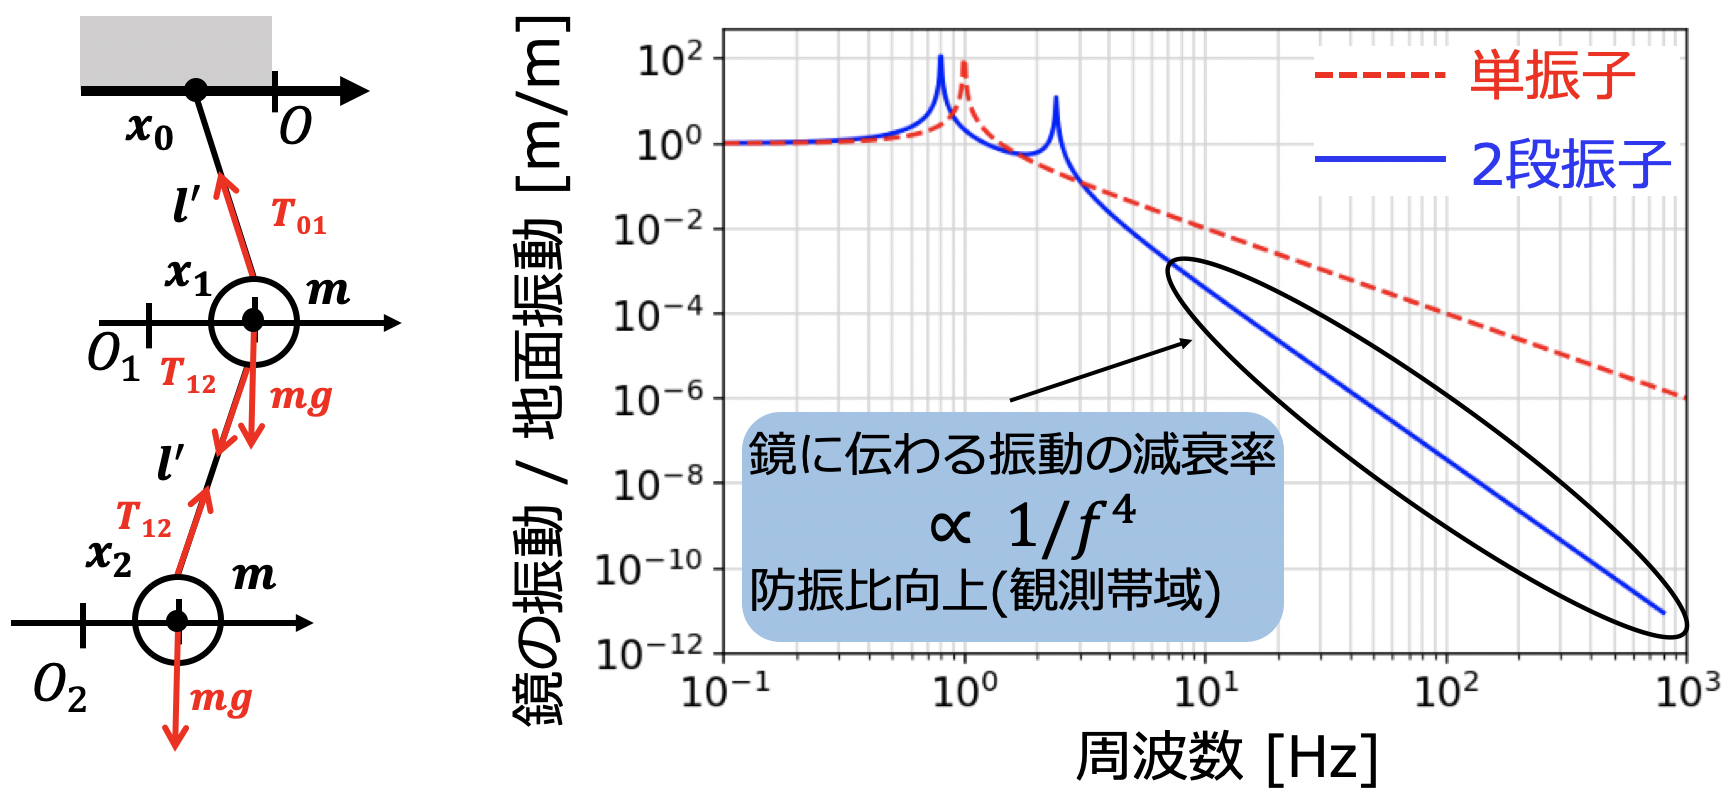
\includegraphics[width=150mm]{fig3_2.png}
\caption[2段振り子のモデルと単振り子との比較]{2段振り子のモデル(左)と, 全長が同じ場合の単振り子・2段振り子の防振比の比較(右). 2段振り子の方が, 観測帯域(10$\sim$数100 Hz)において優れた防振比をもつことが分かる. }
\label{fig3.2}
\end{center}
\end{figure}
そこで, 次は2段振り子を考える. 図\ref{fig3.2}の左に示すように, 質点の質量を$m$, ワイヤ長を$l^{\prime}$, ワイヤの張力を$T_{01},T_{12}$, 質点と地面の変位をそれぞれ$x_1(t),x_2(t),x_0(t)$で表すと, 1段目の質点の運動方程式は
\begin{equation}
\begin{split}
&鉛直方向:0=T_{01,y}-T_{12,y}-mg=T_{01}\times\frac{\sqrt{l^{\prime^2}-(x_1(t)-x_0(t))^2}}{l^{\prime}}-T_{12}\times\frac{\sqrt{l^{\prime^2}-(x_1(t)-x_2(t))^2}}{l^{\prime}}-mg\\
&水平方向:m\ddot{x}_1(t)=-T_{01,x}-T_{12,x}=-T_{01}\times\frac{x_1(t)-x_0(t)}{l^{\prime}}-T_{12}\times\frac{x_1(t)-x_2(t)}{l^{\prime}}
\end{split}
\label{eq3.7}
\end{equation}
2段目の質点の運動方程式は
\begin{equation}
\begin{split}
&鉛直方向:0=T_{12,y}-mg=T_{12}\times\frac{\sqrt{l^{\prime^2}-(x_1(t)-x_2(t))^2}}{l^{\prime}}-mg\\
&水平方向:m\ddot{x}_2(t)=T_{12,x}=T_{12}\times\frac{x_1(t)-x_2(t)}{l^{\prime}}
\end{split}
\label{eq3.8}
\end{equation}
1段振り子の場合と同様に, 質点の変位がワイヤ長に比べて十分小さいとすると, 2段目の質点の鉛直方向の運動方程式より
\begin{equation}
0=T_{12}-mg,
\label{eq3.9}
\end{equation}
となり, これを用いると, 1段目の質点の鉛直方向の運動方程式は
\begin{equation}
0=T_{01}-2mg,
\label{eq3.10}
\end{equation}
となる. 式(\ref{eq3.9}), (\ref{eq3.10})を式(\ref{eq3.7}), (\ref{eq3.8})に代入すると両質点の水平方向の運動方程式は
\begin{equation}
\begin{split}
m\ddot{x}_1(t)+\frac{2mg}{l^{\prime}}(x_1(t)-x_0(t))+\frac{mg}{l^{\prime}}(x_1(t)-x_2(t))&=0\\
m\ddot{x}_2(t)-\frac{mg}{l^{\prime}}(x_1(t)-x_2(t))&=0
\end{split},
\end{equation}
Fourier変換してまとめると
\begin{equation}
\begin{pmatrix}
3\omega_0^{\prime^2}-\omega^2 & -\omega_0^{\prime^2}  \\
-\omega_0^{\prime^2} & \omega_0^{\prime^2}-\omega^2  
\end{pmatrix}
\begin{pmatrix}
\tilde{x}_1 \\
\tilde{x}_2
\end{pmatrix}
=
\begin{pmatrix}
2\omega_0^{\prime^2}\tilde{x}_0 \\
0
\end{pmatrix},
\end{equation}
ここで$\omega_0^{\prime}\equiv\sqrt{g/l^{\prime}}$とした. これを解いて, 
\begin{equation}
\frac{1}{\tilde{x}_0}
\begin{pmatrix}
\tilde{x}_1 \\
\tilde{x}_2
\end{pmatrix}
=\frac{1}{\omega^4-4\omega_0^{\prime^2}\omega^2+2\omega_0^{\prime^4}}
\begin{pmatrix}
2(\omega_0^{\prime^4}-\omega_0^{\prime^2}\omega^2)\\
2\omega_0^{\prime^4}
\end{pmatrix}.
\end{equation}
よって防振比は
\begin{equation}
\frac{\tilde{x}_2}{\tilde{x}_0}=\frac{2\omega_0^{\prime^4}}{\omega^4-4\omega_0^{\prime^2}\omega^2+2\omega_0^{\prime^4}}.
\end{equation}
\quad 2段振子の全長が単振り子と同じ場合, 両者の防振比を比較すると図\ref{fig3.2}の右側のようになる. 2段振り子の場合, 共振周波数よりも高い周波数において, 地面から鏡に伝わる振動は周波数の4乗で減衰し, 単振り子と比べて防振比が向上しているのが分かる. 
\subsection{多段振り子}
\begin{figure}[H]
\begin{center}
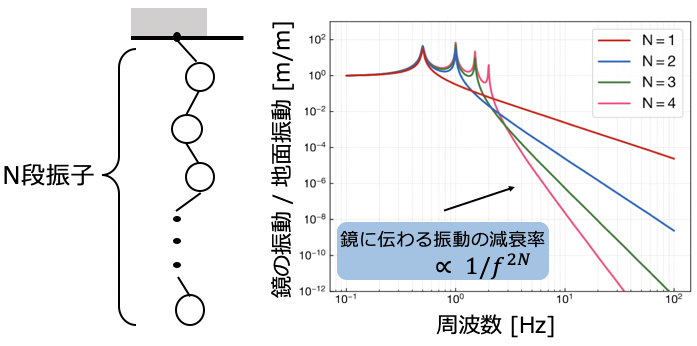
\includegraphics[width=150mm]{fig3_3.png}
\caption[N段振り子のモデルと防振比の比較]{N段振子のモデル(左)と, 防振比の比較(右). 共振周波数以上では地面から鏡に伝わる振動は周波数の2N乗で減衰する. }
\label{fig3.3}
\end{center}
\end{figure}
同様にして, N段振り子の場合も計算する. 質点の質量を$m$, ワイヤ長を$l$, $k$本目のワイヤ($k-1$段と$k$段をつなぐワイヤ)の張力を$T_{k-1,\,k}$質点の変位をそれぞれ$x_1(t),x_2(t),...,x_N(t)$, 地面の変位を$x_0(t)$で表すと$k$段目の質点の水平方向の運動方程式は
\begin{equation}
m\ddot{x}_k(t)=
\begin{cases}
-T_{k-1,\,k}\frac{x_k(t)-x_{k-1}(t)}{l}-T_{k(k+1)}\frac{x_k(t)-x_{k+1}(t)}{l} & (k=1,2,...,N-1)\\
-T_{N-1,\,N}\frac{x_N(t)-x_{N-1}(t)}{l} & (k=N)
\end{cases}.
\end{equation}
先ほどまでと同様に, 水平方向の変位がワイヤ長に比べて十分小さいとすると, 上から$k$本目のワイヤの張力は
\begin{equation}
T_{k-1,\,k}=(N+1-k)mg,
\end{equation}
と書ける. よって, 運動方程式は
\begin{equation}
m\ddot{x}_k(t)=
\begin{cases}
-(N+1-k)\frac{mg}{l}(x_k(t)-x_{k-1}(t))-(N-k)\frac{mg}{l}(x_k(t)-x_{k+1}(t)) & (k=1,2,...,N-1)\\
-(N+1-k)\frac{mg}{l}(x_N(t)-x_{N-1}(t)) & (k=N)
\end{cases},
\end{equation}
と書き換えられる. $\omega_0=\sqrt{g/l}$としてFourier変換し, 式を整理すると
\begin{equation}
\begin{cases}
\left[-\omega^2+(2N-2k+1)\omega_0^2\right]\tilde{x}_k-(N+1-k)\omega_0^2\tilde{x}_{k-1}-(N-k)\omega_0^2\tilde{x}_{k+1}=0 & (k=1,2,...,N-1)\\
\left(-\omega^2+\omega_0^2\right)\tilde{x}_N-\omega_0^2\tilde{x}_{N-1}=0 & (k=N)
\end{cases}.
\end{equation}
つまり
\begin{equation}
A
\begin{pmatrix}
\tilde{x}_1\\
\tilde{x}_2\\
\vdots\\
\tilde{x}_p\\
\vdots\\
\tilde{x}_N
\end{pmatrix}
=
\begin{pmatrix}
N\omega_0^2\tilde{x}_0\\
0\\
\vdots\\
0\\
\vdots\\
0
\end{pmatrix}.
\end{equation}
ただし, $2\leq p\leq N-1$であり, 
\begin{equation}
A=
\begin{pmatrix}
a_{1,\,1}&a_{1,\,2}&0&\cdots&\\
a_{2,\,1}&a_{2,\,2}&a_{2,\,3}&0&\cdots&\\
&&&&\ddots&&&&\ddots\\
&&&&\cdots&0&a_{p,\,p-1}&a_{p,\,p}&a_{p,\,p+1}&0&\cdots&\\
&&&&&&\ddots&&&&\ddots\\
&&&&&&&&&&&\cdots&0&a_{N,\,N-1}&a_{N,\,N}
\end{pmatrix},
\end{equation}
\begin{equation}
a_{1,\,1}=-\omega^2+(2N-1)\omega_0^2,\quad a_{1,\,2}=-(N-1)\omega_0^2,
\label{eq3.21}
\end{equation}
\begin{equation}
a_{p,\,p-1}=-(N+1-p)\omega_0^2,\quad a_{p,\,p}=-\omega^2+(2N-2p+1)\omega_0^2,\quad a_{p,\,p+1}=-(N-p)\omega_0^2,
\label{eq3.22}
\end{equation}
\begin{equation}
a_{N,\,N-1}=-\omega_0^2,\quad a_{N,\,N}=-\omega^2+\omega_0^2,
\label{eq3.23}
\end{equation}
である. よってCramerの公式より
\begin{equation}
x_N=\frac{1}{|A|}|B|.
\end{equation}
ただし、
\begin{equation}
B=
\begin{pmatrix}
a_{1,\,1}&a_{1,\,2}&0&\cdots&&&&&&&&&&0&N\omega_0^2\tilde{x}_0\\
a_{2,\,1}&a_{2,\,2}&a_{2,\,3}&0&\cdots&&&&&&&&&&0\\
&&&&\ddots&&&&\ddots\\
&&&&\cdots&0&a_{p,\,p-1}&a_{p,\,p}&a_{p,\,p+1}&0&\cdots&\\
&&&&&&\ddots&&&&\ddots\\
&&&&&&&&&&&\cdots&0&a_{N,\,N-1}&0
\end{pmatrix}.
\end{equation}
$a_{i,\,j}$の余因子を$A_{i,\,j}$と書くと
\begin{equation}
x_N=\frac{\sum\limits_{i=1}^{N}a_{i,\,N}B_{i,\,N}}{\sum\limits_{i=1}^{N}a_{i,\,N}A_{i,\,N}}.
\end{equation}
ここで0である要素に注意すると
\begin{equation}
x_N=\frac{N\omega_0^2\tilde{x}_0\times\prod\limits_{q=2}^{N}a_{q,\,q-1}}{\prod\limits_{q=1}^{N}a_{q,\,q}+a_{N-1,\,N}A_{N-1,\,N}}.
\end{equation}
さらに式(\ref{eq3.21}),(\ref{eq3.22}),(\ref{eq3.23})に注意すると
\begin{equation}
\frac{\tilde{x}_N}{\tilde{x}_0}=\frac{N\omega_0^2\times(\omega\text{の0次式})}{(\omega\text{の2N次式})},
\end{equation}
である(対角成分の積は$(\omega^2)^N$次式$=\omega$の2$N$次式になる). \\
\quad これより, N段振り子では共振周波数以上において, 地面から鏡に伝わる振動が周波数の2$N$乗で減衰することが分かる. よって, 重力波検出器では必要な防振比を得るために多段振り子を用いており(図\ref{fig3.3}), 特にKAGRAでは9段振り子となっている. 

\section{KAGRAにおける防振懸架系の概要}
この節では, KAGRAで用いられている防振懸架系について記述する. そのために, まずKAGRAの干渉計の構成を示し, その後各懸架系の説明を行う. 
\subsection{KAGRAにおける防振懸架系の位置}
KAGRAの干渉計は, DRFPMIの主要部だけでなく, 多くの光学部品で構成されている. 図\ref{fig3.4}にKAGRAのOptical Layoutを示した. \\
\quad 光源から出たレーザーは増幅機で高出力化され, 空間モード整形とさらなる周波数安定化のために, ミラーを吊り下げた三角共振器であるIMC (Input Mode Cleaner) に送られる. IMCから出た光はFI (Faraday Isolator)\footnote{反射光が逆入してレーザー光源に戻るのを防ぐためのものである. } を通り, 空間モード整形機能を持つIMMT (Input Mode Matching Telescope) で拡大されて干渉計の主要部に送られる. \\
\quad 干渉計の主要部となるのは, 長さ3 kmの2本のアームからなるDRFPMIである. アーム共振器はそれぞれXアーム, Yアームと呼ばれ, ITMとETMで形成されている. 入射ビームはBSで垂直な2方向に分割され, アーム共振器に送られる. そしてアーム共振器からの反射ビームはBSで再結合し, 干渉した光はsymmmetric portと呼ばれる入射方向へ戻っていく. \\
\quad また, symmetric portではPRMがビームを再びアーム共振器に反射させることで, PRMとITM(ITMXとITMYのBSからの平均距離に位置する仮想ITM)で形成されるPRCでパワーを蓄積し, アーム共振器内の実効パワーを増幅させる. 同様に, マイケルソン干渉計の出力側(anti-symmetric port)にもSRCが実装されている. 観測時には干渉光は暗く保たれるが, 重力波到来時はanti-symmetric portから微量のパワーが漏れ出す. この漏れた光子をアーム共振器に戻し, 観測帯域の調整を行う. \\
\quad 最後にSRCから漏れたビームはOMMT (Output Mode Matching Telescope) で空間モード整形とビーム半径の縮小がなされ, OMC (Output Mode Cleaner) を通ってPDで検出される. 
\begin{figure}[H]
\begin{center}
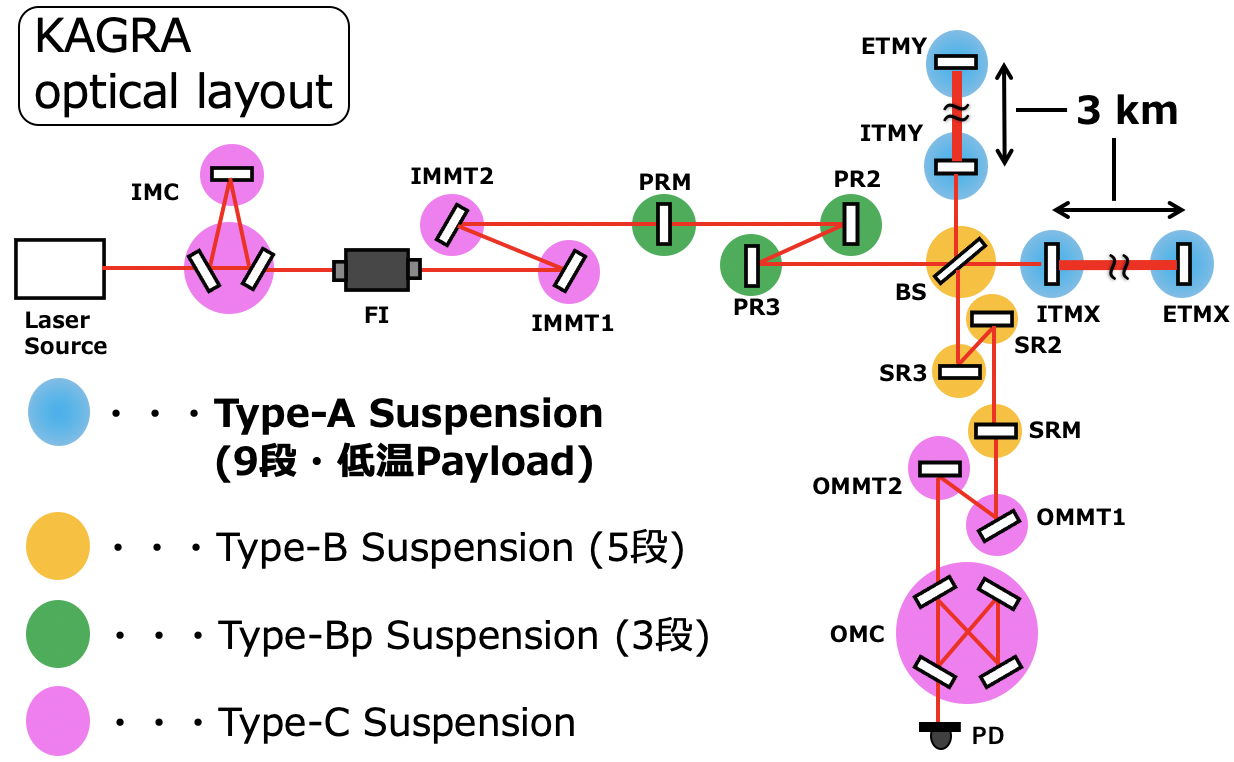
\includegraphics[width=170mm]{fig3_4.png}
\caption[KAGRAのOptical Layout]{KAGRAのOptical Layout}
\label{fig3.4}
\end{center}
\end{figure}
\subsection{防振懸架系}
このようにKAGRAの主干渉計は多数の光学系で構成されており, 防振懸架系についても主にType-A, Type-B, Type-Bpの3種類がある. \\
\quad Type-A Suspensionはサファイア鏡(テストマス)を吊るすための防振懸架系で, 全9段・高さ13.5 mと3種類の中でも最大となっている. これはサファイア鏡の局所運動がアーム長の変化に直接関わるため, 最も高い防振比が要求されるからである. また, 9段の内, 上部の5段はTowerと呼ばれる. 一方, サファイア鏡を含む下4段は低温懸架装置 (Crygenic Payload) と呼ばれ, 20 Kという極低温に冷却される. Type-A Suspension(特に低温懸架装置)は本論文の主な対象であるため, 第\ref{第4章}章で詳細を記す. \\
\quad Type-B SuspensionはBSとSRM, SR2, SR3に使用される2番目に大きな防振システムである. IP (Inverted Pendulum) を含む5段の懸架系であり, 室温で運用される. \\
\quad Type-Bp SuspensionはType-Bを縮小した3段の懸架系で, PRM, PR2, PR3に使用される. IPはないがPayload部分の設計はType-Bと同じで, 室温で運用される. 
\begin{figure}[H]
\begin{center}
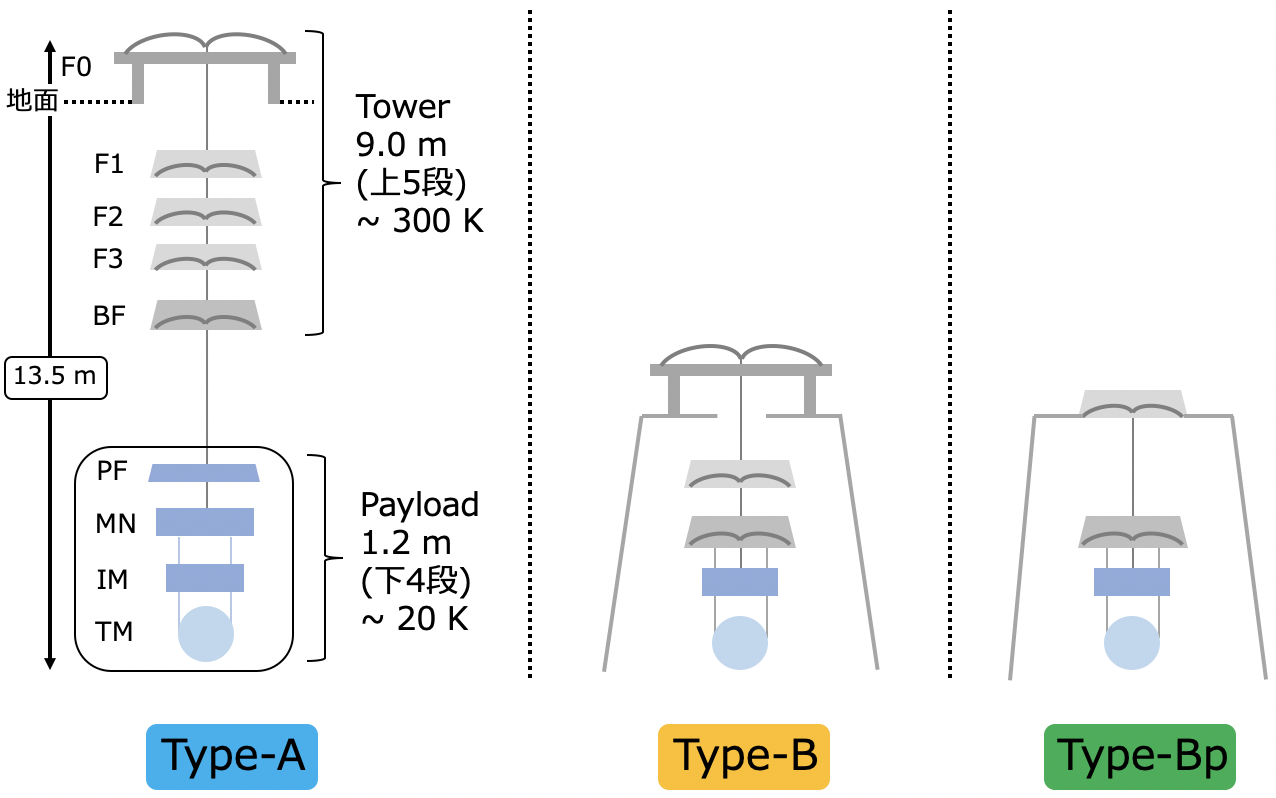
\includegraphics[width=140mm]{fig3_5.png}
\caption[3種類の懸架系]{主干渉計で用いられる3種類の懸架系の概略図}
\end{center}
\end{figure}
\subsection{干渉計の制御フェイズと要求値}
\begin{figure}[H]
\begin{center}
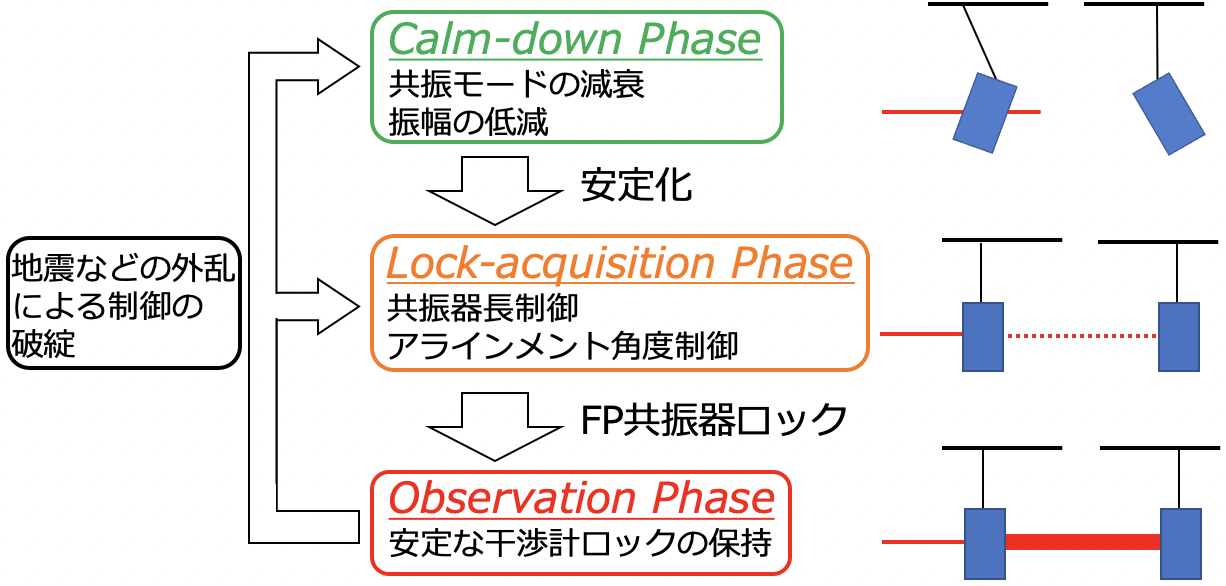
\includegraphics[width=150mm]{fig3_6.png}
\caption[干渉計の制御フェイズ]{干渉計の制御フェイズ}
\label{fig3.6}
\end{center}
\end{figure}
防振懸架系の観点から考えると, 干渉計の安定動作のためには, 懸架系の機械的共振による鏡の過大な揺れを抑える必要がある. KAGRAではそのような振動抑制のためにアクティブ制御を行っている. 防振懸架系に対するアクティブ制御では, まずセンサによって懸架系の動きを検知する. その後, デジタルサーボシステム上で適切なフィルタをかけ, その信号を非接触のアクチュエータによって系にフィードバックしている. \\
\quad このようなアクティブ制御は, 安定な動作のためにサーボの設計に工夫が必要などの難点がある. しかし, 懸架系をインストールした後であっても下記の干渉計フェイズに合わせて制御法を変えることができ, その柔軟性が大きな利点である. \\
\quad ここで, 重力波干渉計はいきなり観測状態を作り出せるわけではない. まず, 懸架された鏡の揺れを抑えて安定化し, それから共振器の長さや角度の制御を行うというように, 段階を追いながら観測可能な状態にする必要がある. これについて, KAGRAにおける干渉計の制御フェイズは懸架系の観点から, Calm-down, Lock-acquisition, Observationの3つに分類される. これらのフェイズ間の遷移を図\ref{fig3.6}に示す. \\
\quad Calm-downフェイズは, 鏡が大きな振幅で揺れて干渉計のアライメントが保てなくなり, 有意な信号が出なくなった状態である. この段階では鏡の振動を抑制してノミナル位置に戻し, ロックを開始できるようにする必要がある. なお, ロックとは一般に物理量を目的の値に制御して保持することを指し, この場合はFP共振器を共振状態に保つことを表している. また, この段階では, 制御ノイズの削減よりも大きな外乱に対するロバスト性が重要視される. つまり機械的共振のモード減衰が重要となり, ここでは振動が1/eに収まる時間が60秒以下であることが要求される. \\
\quad 次にLock-acquisitionフェイズとは, FP 共振器を共振状態にロックして観測準備を行う段階である. 干渉計信号の線形領域は非常に小さいため, このフェイズで鏡の速度を十分小さくする必要がある(L方向 $<$240 $\mu$m/s). また, より感度の高い干渉計センサを用いた制御ループの作動のために, WFS (Wave Front Sensor) \cite{35}など, 角度変動を抑えるような局所的な制御も必要である(P,Y方向 $<$880 nrad). これは共振器を構成する鏡は3 km離れており, 小さな角度変化でも干渉計には大きな影響を与えるからである. なお, 懸架系の自由度については次節に記した. \\
\quad 最後のObservationフェイズは干渉計の全共振器をロックし, 重力波観測を行う段階である. ここで最も重要なのは, より良い感度で観測を行うために制御ノイズを小さくすること, および安定した運転のために鏡の変位や向きをある範囲に保つことである. 

\subsection{懸架系の自由度}
\ref{sec3.1}節では1次元運動について記述したが, 本来は3次元の剛体を考えるべきである. そこで全部で6つの自由度 (DoF:Degree of Freedom) を図\ref{fig3.7}に示した通りに定義する(並進軸:Longitudinal, Transverse, Vertical, 回転軸:Roll, Pitch, Yaw). 3つの並進軸は右手系を成し, 3つの回転軸は並進軸周りの右ねじの回転が正方向となるように定義されている. 本論文では, これら6つの自由度を(L, T, V, R, P, Y)のように頭文字をとって略記することがある. \\
\quad 光共振器や干渉計の構成にはビーム軸方向だけでなく, 他の自由度の運動も非常に重要である. L方向の運動は光路長の変化に直結し, PとYの回転はビームアライメントに影響する. また, TとV方向の運動はビームのセンタリングに関わる. 
\begin{figure}[H]
\begin{center}
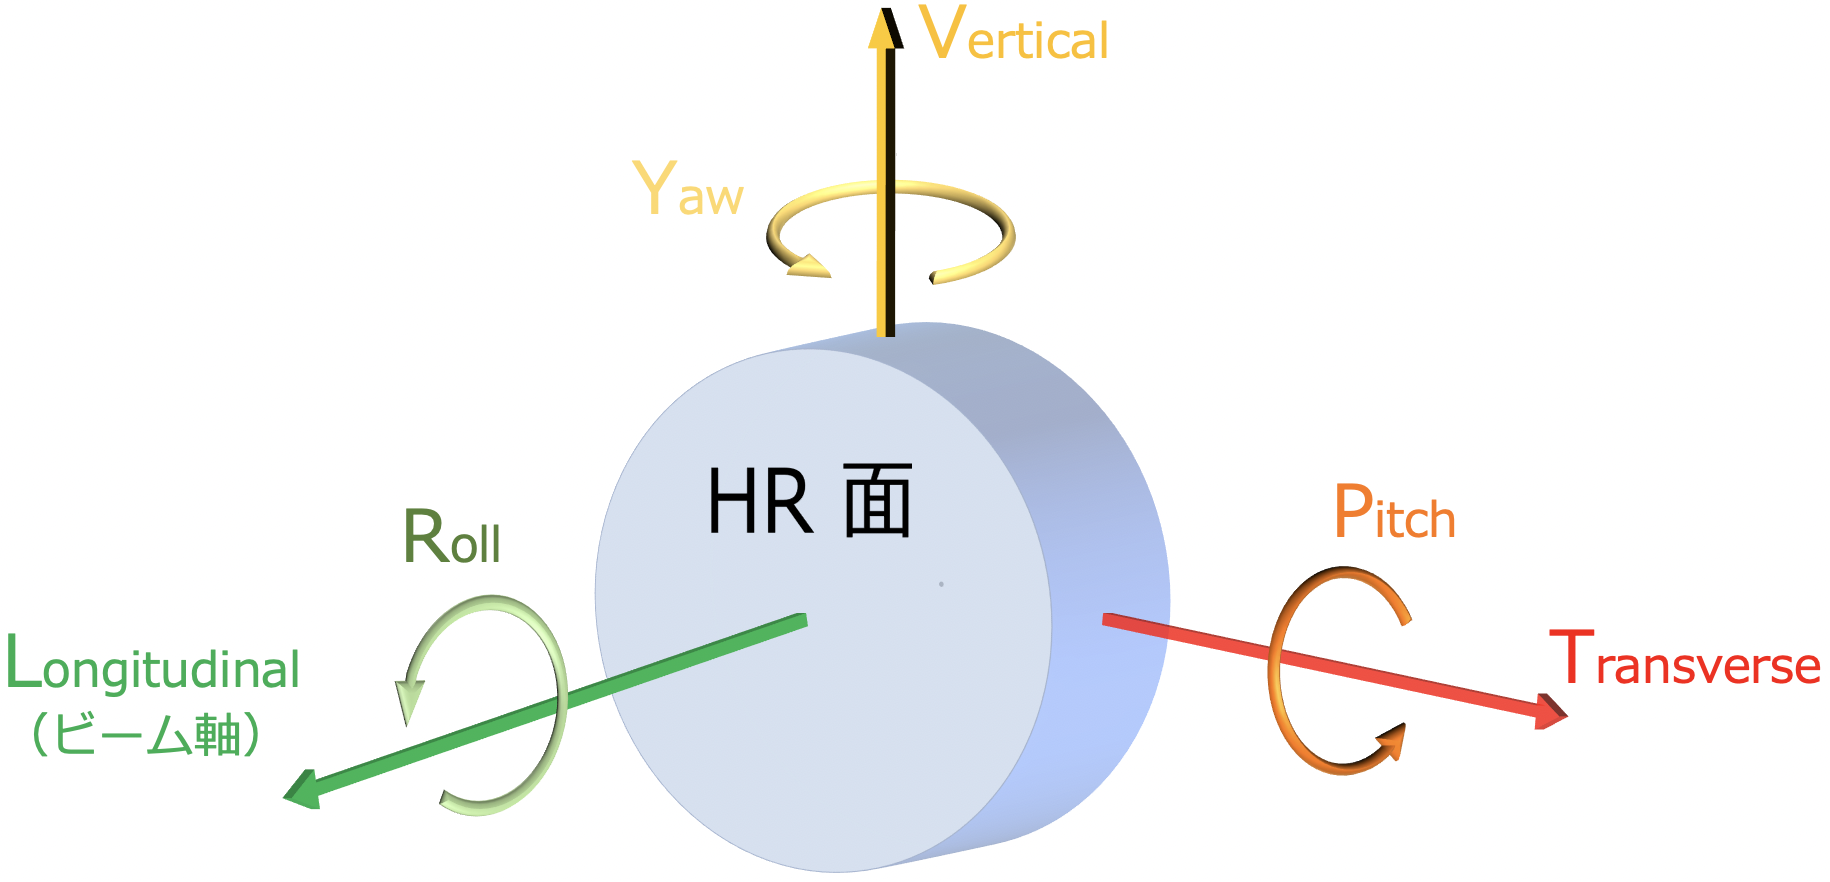
\includegraphics[width=150mm]{fig3_7.png}
\caption[懸架系の運動の自由度]{懸架系の運動の自由度の定義. HR面は高反射率コーティングを施した面を示す. 本論文では, これら6つの自由度を(L, T, V, R, P, Y)のように頭文字をとって略記することがある. }
\label{fig3.7}
\end{center}
\end{figure}

\chapter{KAGRA Type-A Suspension}
\label{第4章}
\fontsize{11pt}{16pt}\selectfont
先の章で述べたようにType-A Suspensionは大きく分けてType-A Towerと低温懸架系 (Cryogenic Payload) からなる9段の振り子である(図\ref{fig4.1}). この章ではTowerおよび低温懸架系部分の各ステージや用いられるセンサ・アクチュエータについて詳細を記述する. 
\begin{figure}[H]
\begin{center}
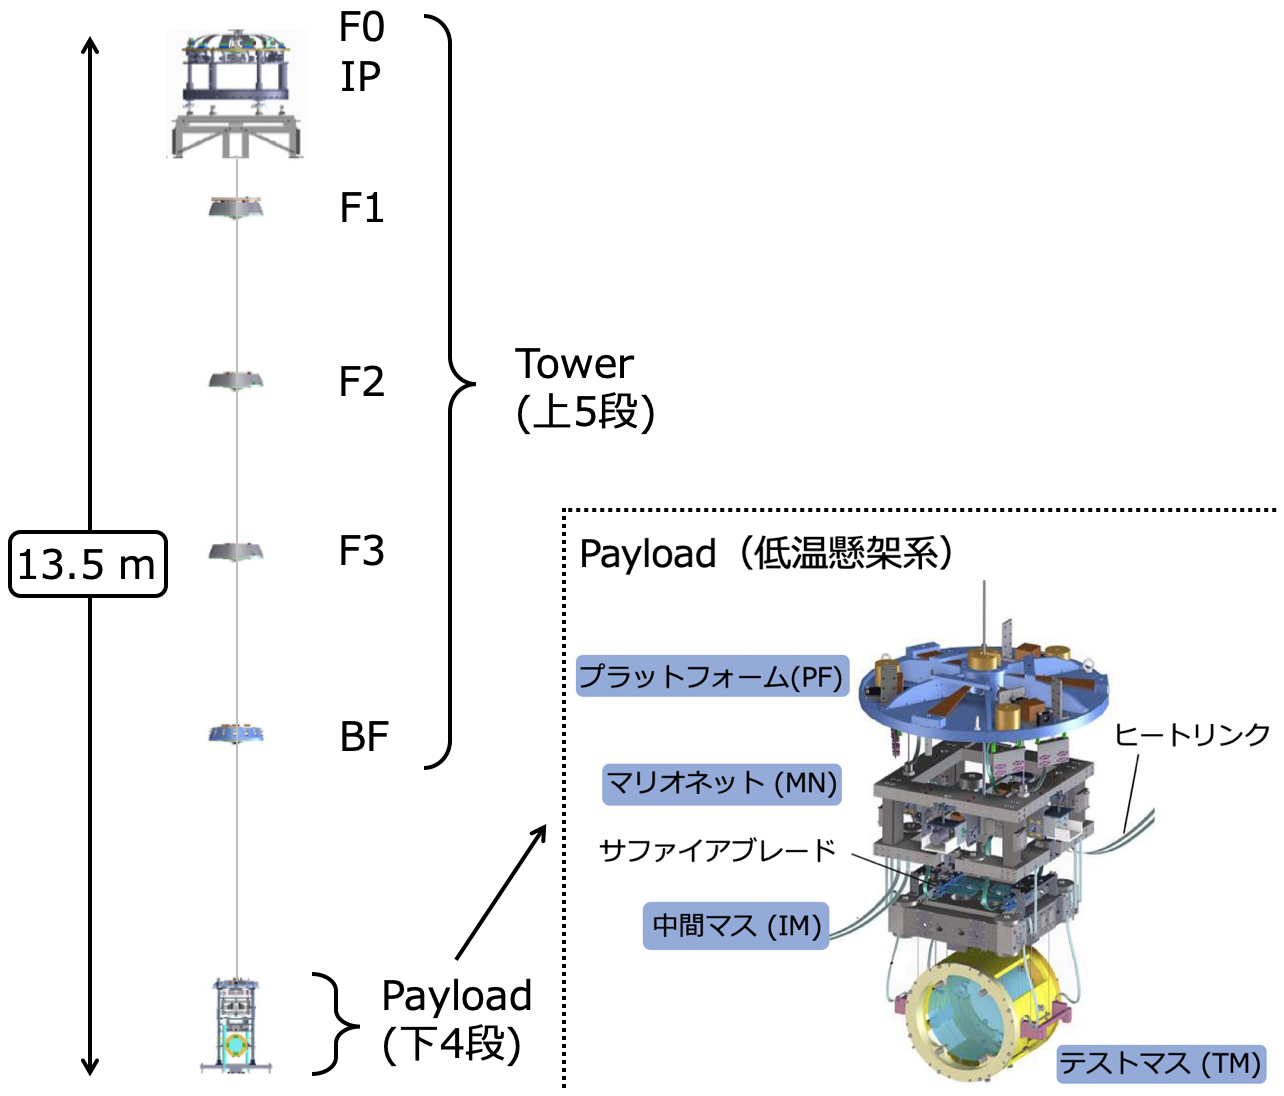
\includegraphics[width=150mm]{fig4_1.png}
\caption[Type-A Suspensionの全体図および低温懸架系部分]{Type-A Suspensionの全体図(左)および低温懸架系 (Cryogenic Payload) 部分(右下)}
\label{fig4.1}
\end{center}
\end{figure}

\section{Type-A Tower}
\subsection{機構}
Type-A Towerは主に1 Hz以下の低周波防振のための部分である. その構成について, IP pre-isolationステージは, 3本のIP (Inverted Pendulum) で支えられている. また, GASフィルタチェーンはトップステージに取り付けられたトップフィルタ(F0)から始まり, フィルタ1, 2, 3(それぞれF1, F2, F3)と名付けられた後続のステージが続き, BF (Botom Filter: ボトムフィルタ) と呼ばれる5段目で終了する. IPおよびGASの仕組みについては補遺\ref{補遺A}に記載した. 
\subsubsection{IP pre-isolation ステージ}
\vskip3mm
IP pre-isolationステージはプレアイソレータと呼ばれIP, ベースリング, トップGASフィルタ($\rm{F_0}$)で構成されている(図\ref{fig4.2}). このステージは0.1Hz以下の低周波からの防振, および防振懸架系全体の位置制御という役割を持つ. 
\begin{figure}[H]
\begin{center}
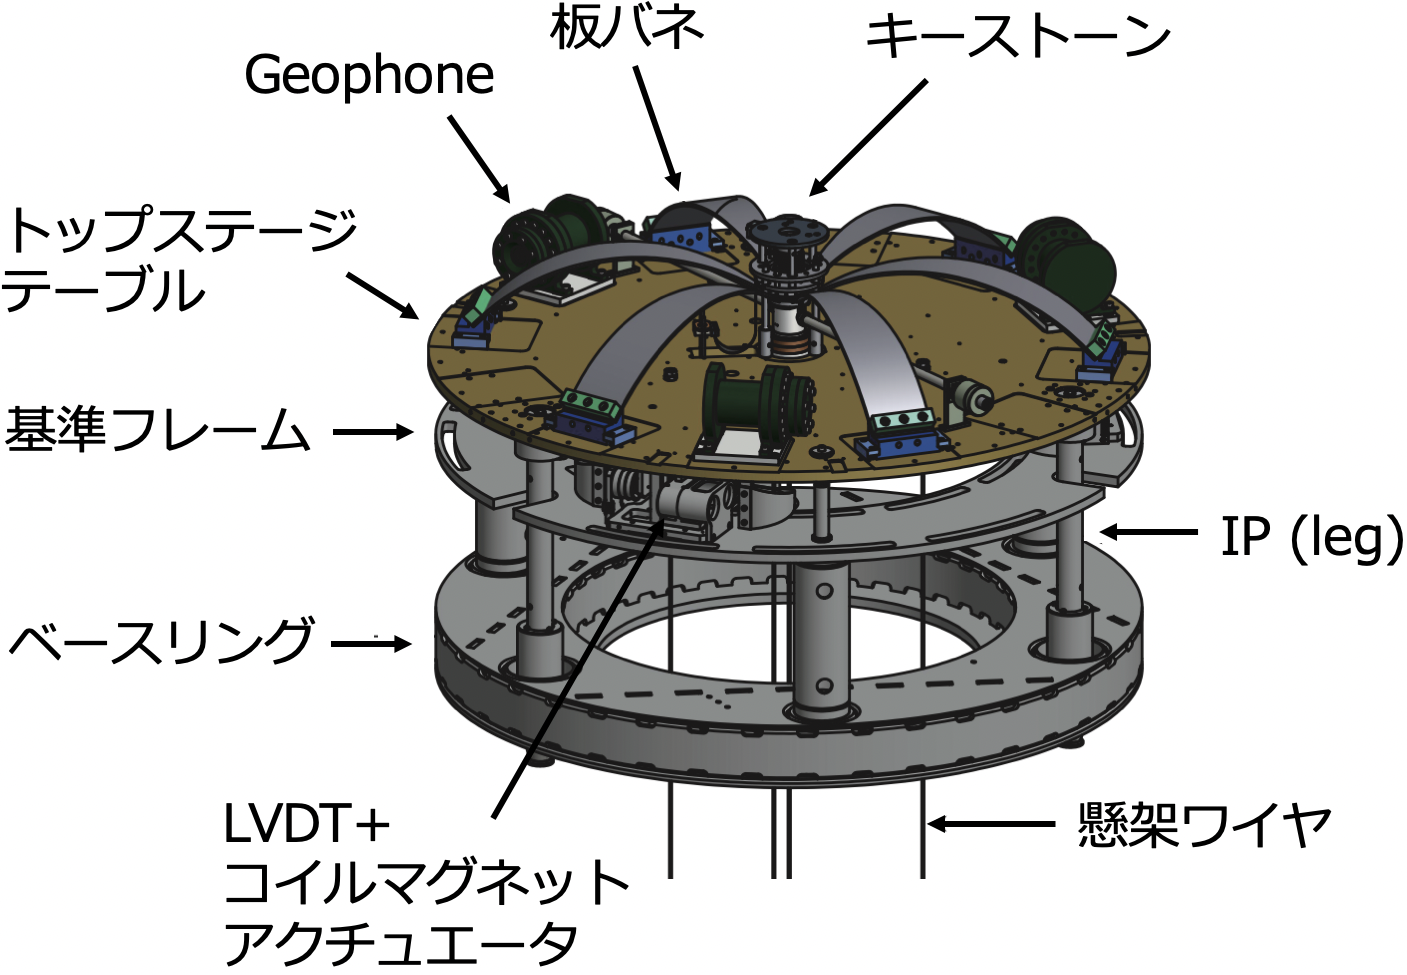
\includegraphics[width=130mm]{fig4_2.png}
\caption[IP pre-isolation ステージ]{IP pre-isolation ステージ(プレアイソレータ)}
\label{fig4.2}
\end{center}
\end{figure}
トップステージは3本のIPの脚で120$^{\circ}$ごとに支持されている. それらの間に位置する3本の支柱はベースリングと基準フレームを接いでおり, そこにLVDTとコイルマグネットアクチュエータのユニットが取り付けられている. また, 地面の揺れに依存しない慣性センサとして, 逆真空容器に収納されたgeophoneがトップステージに搭載されている. なお板バネの先端はトップフィルタの中央にあるキーストーンに接続されている. メインチェーンの懸架ワイヤの1本はこのキーストーンに繋がれており, 他の3本のmagnet damper用ワイヤはトップステージテーブルに直接接続されている. \\
\quad IPの脚は高さ520 mmであり, VirgoのSuper Attenuator\cite{Virgo}に使用されている高さ6mのものと比べてはるかに小さい. このIPは, 脚の中空円筒の両端にフレクシャ接合部を有している. フレクシャ接合部には, 優れた強度と靭性を持つマレージング鋼が使用され, 最上段の変位に伴う強固な弾性屈曲が可能になっている. 各IPはコーンベローズの上に立てられた上でスクリュージャッキにより支えられ, 高さを調節することで接地面を水平にしている. \\
\quad $\rm{F_0}$については, その構造と機能が他のGASフィルタと同様であるため, 次の小節で説明する. また, センサおよびアクチュエータについても後ほど記述する. 
\subsubsection{GASフィルタチェーン}
\label{sec4.1.1.2}
\vskip3mm
Type-A Suspensionには, 水平方向と垂直方向の両方の地面振動減衰を満たすために5段のGASフィルタチェーンがインストールされている. 最上段に実装されたGASステージはトップGASフィルタと呼ばれ, 続く3段はよりコンパクトな設計のGASフィルタ(標準GASフィルタ)になっている. なお, Tower部分の最終段はBF (Botom Filter) と呼ばれ, 基本的には標準GASフィルタと同じ機構だが, BFはTowerと低温懸架系の間のインターフェイスとして重要な機能を持つため, 区別されている. 
\begin{figure}[H]
\begin{center}
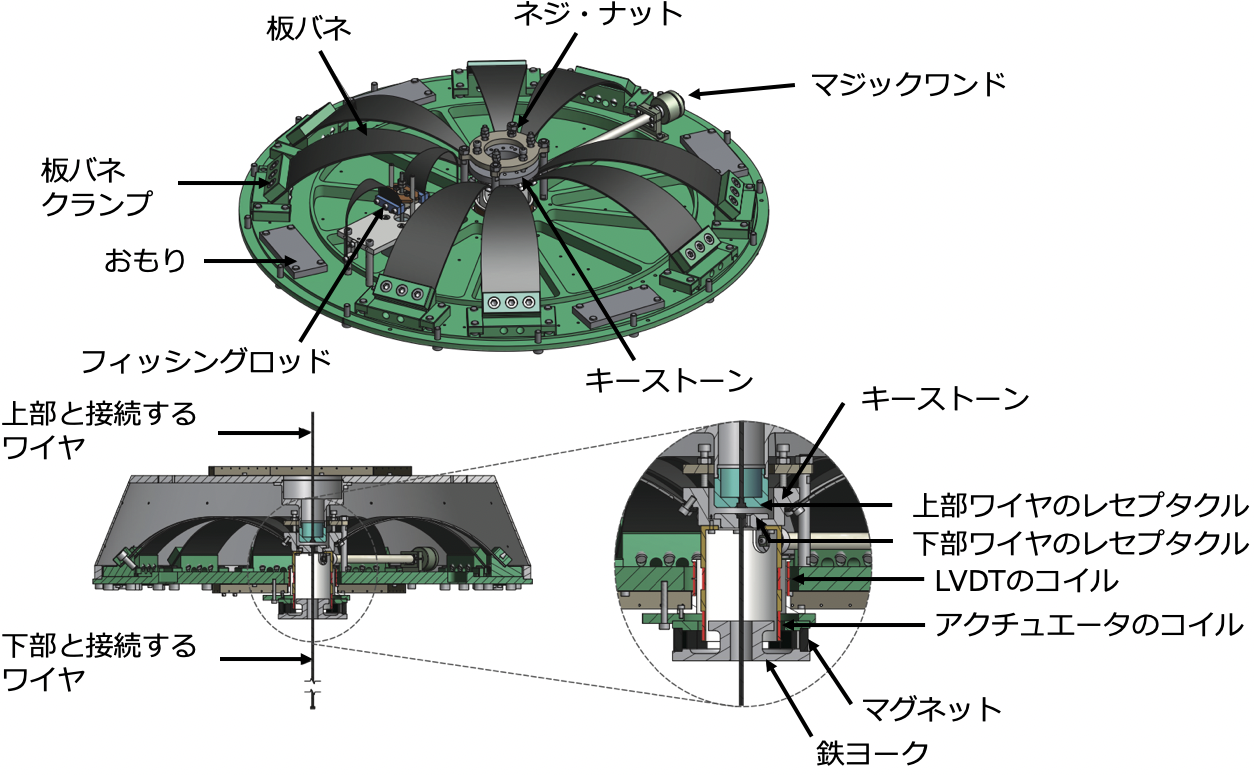
\includegraphics[width=160mm]{fig4_3.png}
\caption[GASフィルタ]{GASフィルタ}
\label{fig4.3}
\end{center}
\end{figure}
標準GASフィルタ($\rm{F_1},\rm{F_2},\rm{F_3}$)の基本構造は, 図\ref{fig4.3}に示すように円盤状のベースプレート上に実装されている(動作原理については補遺\ref{補遺A}に記した). 二等辺三角形の板バネが放射状にベースプレートに取り付けられており, 曲げられた板バネの先端は下段用の懸架ワイヤーが引っ掛けられるキーストーンに固定されている. これにより生まれる軸対称の制約から, キーストーンは垂直方向にのみ振動することができる. なお, その上下振動はLVDT変位センサでモニターしてコイルマグネットアクチュエータで制御している. また, 上段からのワイヤは三角錐型キャップの中心で引っ掛けられ, その半径方向の端でネジによってベースプレートに固定される. キーストーンとワイヤレセプタクルは懸架位置が質量中心に近くなるように配置されており, さらにキーストーンには振動中心を補正するためのマジックワンドが取り付けられている. \\
\quad また, 各板バネは曲がった状態で均一な応力分布になるように設計されている. さらに, その幅・厚み・枚数は, その最適荷重がステージからの吊り下げ重量と等しくなるように調整されている. 表\ref{table4.1}に示した通り, 重い荷重を支えるステージほど, 所定の共振周波数を得るために大きな反バネ効果が必要となるため, $\rm{F_0}$は板バネが厚く, また標準GASフィルタは上部のものほど板バネの枚数が多くなっている. 
\begin{table}[H]
 \centering
  \begin{tabular}{cccc}
   \hline\hline
    & 厚み [mm] & 最大幅 [mm] & 板バネの枚数 \\
   \hline 
   $\rm{F_0}$ & 5.0 & 125 & 6 \\
   $\rm{F_1}$ & 2.4 & 80  & 12 \\
   $\rm{F_2}$ & 2.4 & 80  & 10 \\
   $\rm{F_3}$ & 2.4 & 80  & 8 \\
   BF         & 2.4 & 80  & 5 \\
   \hline
  \end{tabular}
 \caption[GASフィルタの板バネのパラメータ(Type-A)]{GASフィルタの板バネのパラメータ(Type-A). $\rm{F_1,F_2,F_3}$が標準フィルタである}
 \label{table4.1}
\end{table}
\subsubsection{BF}
\vskip3mm
BFは, Type-Aサスペンションのタワー部にある最後のGASステージである. 基本的な機械設計は標準GASフィルタと同じだが, TowerとCryogenic Payloadのインタフェースとして特別な機能をいくつか持っている. \\
\quad BFの重要な役割の1つとして, 懸架系の下部において比較的大きな作動範囲の制御を行うことが挙げられる. このステージにはセンサ (BF LVDT) とアクチュエータが一体となったBF damperと呼ばれる装置が搭載されており, 地面に対するBFの動きを6自由度で測定し制御することができる. BFでは, アクチュエータから発生するノイズが鏡に伝わりにくいため, Payloadよりも大きな作動範囲を実現することができるのである. \\
\quad また, BF damperは単線懸架系のねじれ運動を減衰することができる. 懸架系のねじれは, 並進方向の地面振動と連動して発生する. そのためY方向には低周波の機械的共振によって十分な減衰が得られるので, 干渉計の感度に関わるノイズという観点ではねじり振動はあまり問題にならない. しかし, 懸架系がキックされてY方向の振動が励起されると減衰するのに長い時間を要し, 鏡の位置がずれて干渉計のデューティサイクルが低下する. BFの位置は基本Yモードのノード(上部のGASフィルタの懸垂点)から離れているため, BF damperを作動させることによって効果的なダンピングを適用できる. 
\subsection{センサ・アクチュエータ}
\ref{sec3.1}節で振り子による受動防振について述べた. しかし, 受動防振は共振周波数より高い周波数帯において地面振動の影響を抑えるものであり, 共振周波数付近およびそれ以下の帯域では能動防振が必要になる. これはセンサで読み取った振動を, アクチュエータで力を加えることにより減衰させるものである. 能動防振はセンサ・制御フィルタ・アクチュエータから成るが, この節ではType-A Tower部分で用いられるセンサおよびアクチュエータについて述べる(低温懸架装置で用いられるセンサ・アクチュエータは\ref{sec4.2.2}節, また制御フィルタについては第\ref{第6章}章参照). 
\subsubsection{LVDT}
\vskip3mm
LVDT (Linear Variable Differential Transducer) は誘導結合したコイル間の変調磁界を利用した相対変位センサであり\cite{36}(図\ref{fig4.4}), IPやGASフィルタの動きを読み取っている. その動作原理は次の通りである. \\
\quad 1次コイルに約10 kHzの正弦波変調信号を送ると, その周囲に振動磁界が発生する. そして, その磁界の変化を同軸上に置かれた2次コイルが感知し, 誘導電圧を発生させる. 2つの2次コイルは互いに逆巻きなので, 1次コイルを2次コイルの中心に置くと誘導電圧は打ち消される. ここで, 1次コイルが中心からずれると相互インダクタンスが変化し, 誘導電圧の差動がその後の読み出しで正味の電圧として現れる. この差動電圧は増幅されてミキサーに送られ, ミキサーはこの振動電圧を復調して1次コイルの変位(低周波信号)を得る. \\
\quad LVDTの特徴は変位に対する線形応答が, 軸方向の大きなダイナミックレンジで得られることである. KAGRAではそのダイナミックレンジはcm, 分解能はsub$\mu$mであるが, その具体的な値は用途によって決められる. KAGRA懸架系のシステムには, IPやGASフィルタに使用される標準的なLVDTとBFに使用される専用のLVDTの2種類があり, 後者についてはLVDTの2次コイルをアクチュエータコイルと共用する設計である. 
\begin{figure}[H]
\begin{center}
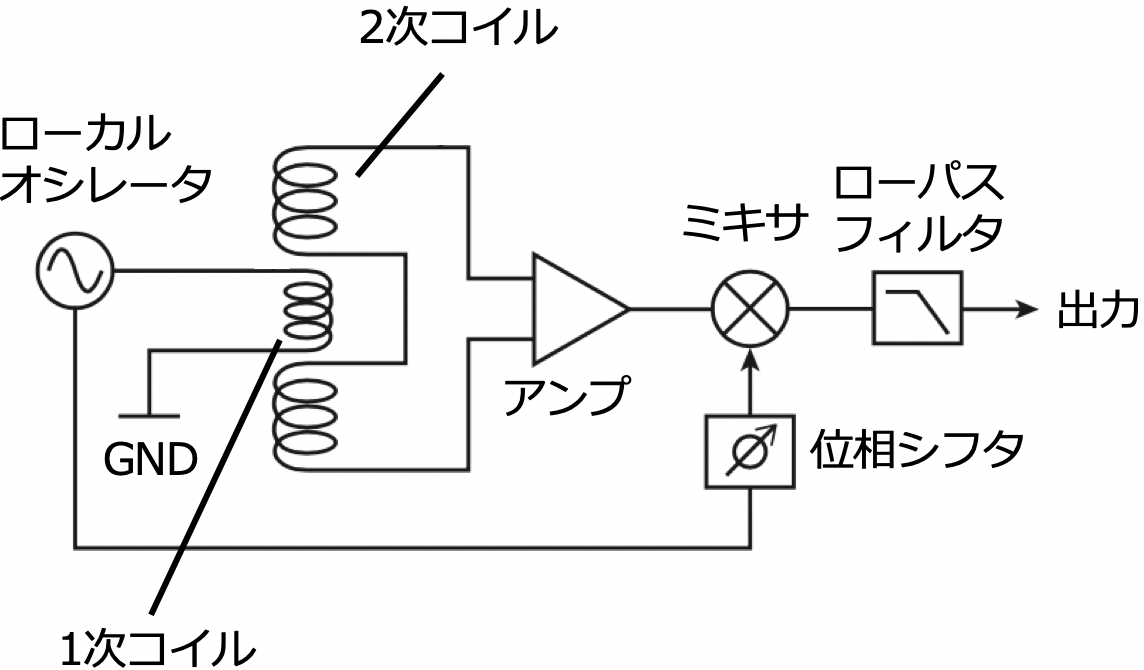
\includegraphics[width=130mm]{fig4_4.png}
\caption[LVDTの概要図]{LVDTの概要図}
\label{fig4.4}
\end{center}
\end{figure}
\subsubsection{Geophone}
\vskip3mm
Geophoneは慣性系に対する速度を測定する装置であり, LVDTと同様IPの動きをモニターする. 2種類のセンサを用いているのは, 感度が良い帯域が両者で異なるからである. 具体的には, GeophonはLVDTに比べ高い周波数で感度が良い. そのため, クロスオーバー周波数(両者のゲインの大小が入れ替わる周波数)が約0.1 HzとなるようにLVDTの信号にローパスフィルタを, Geophoneの信号にハイパスフィルタをかけてIPの制御を行っている. 図\ref{fig4.5}はその制御の様子を示したものである. LVDTのみによる制御(赤)では共振が抑えられているものの, 0.3 Hz以上でノイズが見られる. Geophoneを合わせることにより, そのノイズの影響が抑えられている(水色). 
\begin{figure}[H]
\begin{center}
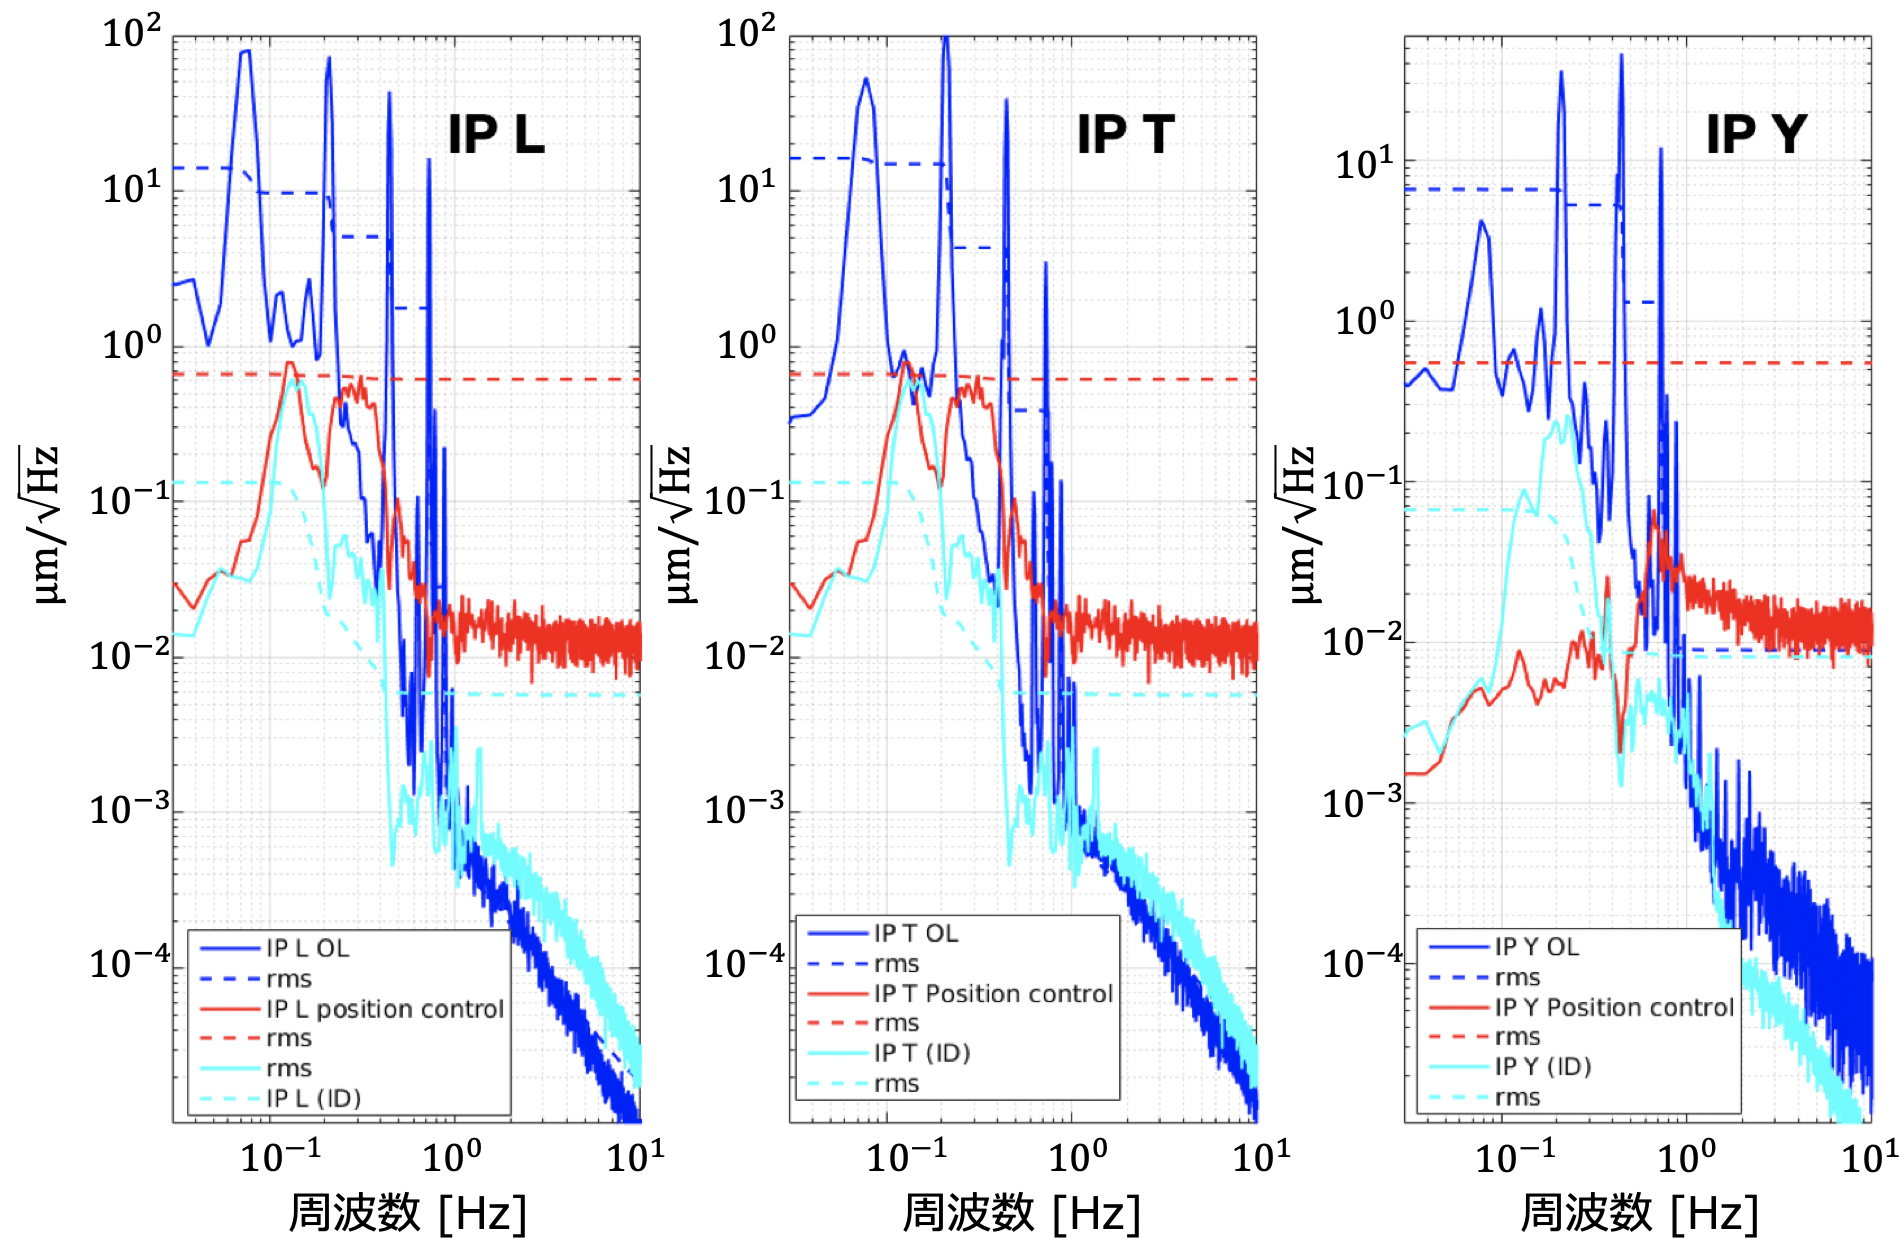
\includegraphics[width=160mm]{fig4_5.png} 
\caption[LVDTとGeophoneによるIPの制御]{LVDTとGeophoneによるIPの制御\cite{37}. 赤線はLVDTのみによる制御を示しており, 共振は抑えられているものの, 0.3 Hz以上でノイズが見られる. これにGeophoneを合わせた制御が水色であり, ノイズの影響が抑えられているのが分かる.}
\label{fig4.5}
\end{center}
\end{figure}
KAGRAではSercel社製のL-4Cを用いている. これはプルーフマスの筐体に対する速度に比例して電圧を出力するが, その動作原理は次の通りである. \\
\quad 約1 kgのプルーフマスはバネおよびdamperで吊り下げられており, コイルが巻き付けられている(共振周波数は1 Hz). そしてこのコイルが筐体に取り付けられた永久磁石による誘導電圧を発生させる. geophoneは特定の光や電波等の補助を必要としない受動計測装置であり, 内部発振器の制御を必要としないため設置やメンテナンスが容易である. \\
\quad generator定数$G_{\rm e}$, 減衰係数$\eta$, 角周波数$\omega$および角共振周波数$\omega_0$を用いるとgeophoneの周波数応答は
\begin{equation}
H_{\rm geo}(\omega)=\frac{G_{e}\omega^2}{\omega_0^2+2i\eta\omega_0\omega-\omega^2}.
\end{equation}
これよりgeophoneは共振周波数1 Hz以上では平坦な応答を示すが, それ以下の周波数では$f^2$に比例した周波数依存性を示すことが分かる(図\ref{fig4.6}). また, 各パラメータの典型的な値については表\ref{table4.2}の通りである. なお, これらのパラメータは, 複数種類の地震計による同時測定によって校正される. 特に, KAGRAでは地下施設の環境地震モニターとしてNanometrics社のTrillium Compactを2台, Trillium 120QAを1台使用している. これらは広帯域(0.01$\sim$10 Hz)でフラットな応答特性を持つため, 校正が簡単である. \\
\quad geophoneからの出力電圧は信号対雑音比を良くするために前置増幅器回路(プリアンプ)で増幅され, 制御システムに送られる. このとき, 雑音電圧が少ないオペアンプCS3002を用いた第1増幅段階で信号を374.5倍に拡大し, 第2増幅段階で2.5倍に増幅する. よって, 前置増幅器は合計約940 倍の増幅を行うことになる. なお, KAGRAではVirgo用にNikefで設計された前置増幅器回路を用いている. \\
\quad 一方, 前置増幅器はgeophoneの感度を制限するノイズを生む. 雑音電圧の測定結果より, 高周波(0.3 Hz以上)ではジョンソンノイズ(抵抗からの熱雑音), 低周波(0.3 Hz未満)では電流雑音(オペアンプからのノイズ)からの寄与があることが分かっている\cite{38}. 
\begin{figure}[H]
\begin{center}
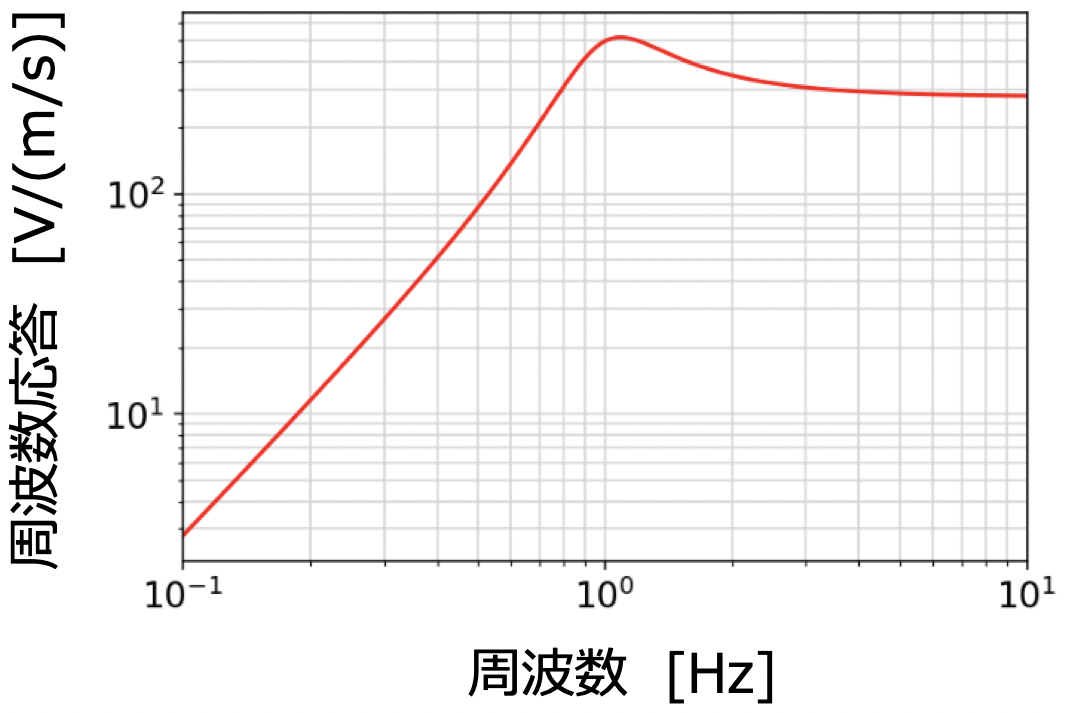
\includegraphics[width=120mm]{fig4_6.png} 
\caption[geophoneの周波数応答]{geophoneの周波数応答(フレーム速度から出力電圧への変換効率)}
\label{fig4.6}
\end{center}
\end{figure}
\begin{table}[H]
 \centering
  \begin{tabular}{cc}
   \hline\hline 
   generator constant & 276.8 V/(m/s) \\
   プルーフマスの重量 & 1 kg \\
   共振周波数         & 1 Hz \\
   減衰定数           & 0.28 \\
   コイルの抵抗       & 5500 $\Omega$ \\
   \hline
  \end{tabular}
 \caption[geophone (L-4C)の各パラメータ]{geophone (L-4C)の各パラメータ(典型的な値)}
 \label{table4.2}
\end{table}
また, geophoneと前置増幅器は大気中で動作させる必要があるが, 懸架系全体は真空中にある. そこで, geophoneの真空適合性を確保するため, ステンレス製の真空ポッドにgeophoneを封入して内部を大気圧に保った. なお, 真空ポッドからの空気漏れが数ヶ月のスケールで無視できることは, \cite{38}で示されている. また, 真空ポッド内のジオフォンの相対位置は, 読出信号に不要なインパルスを発生させる内壁のガタつきを防ぐため, ゴムリングで固定されている. このゴムリングの減衰効果は無視できるほど小さく, geophoneと真空ポッドの筐体は一体であると見なすことができる. 
\subsubsection{Folded Pendulum 加速度計}
\vskip3mm
LVDTとGeophoneを組み合わせてIPの制御を行うと述べたが, 図\ref{fig4.5}を見ると0.1 Hzあたりでの振動減衰は, IPのセンサへの要求値(0.1 Hzにおいて$10^{-7.8}$ m/$\sqrt{{\rm Hz}}$)に対して不十分である. これはGeophoneが低周波における感度が悪いため, クロスオーバー周波数を0.19 Hzまでしか下げられなかったことによる. \\\quad そこで, ノイズが要求に対して十分小さいことが先行研究\cite{FP}によって示されたFP (Folded Pendulum) 加速度計をインストールした. FP加速度計ではプルーフマスの一端を正立振り子で吊るし,もう一端を倒立振り子で支えている. 図\ref{fig4.7}はFP加速度計の概念図であり, このモデルでは質量$M_1$, 長さ$L_1$の正立振り子と質量$M_2$, 長さ$L_2$の倒立振り子が質量のない剛体梁で接続されている. この系の共振周波数は
\begin{equation}
\omega_0=\sqrt{\left(\frac{M_1}{L_1}-\frac{M_2}{L_2}\right)\frac{g}{M_1+M_2}+\gamma}.
\end{equation}
\begin{figure}[H]
\begin{center}
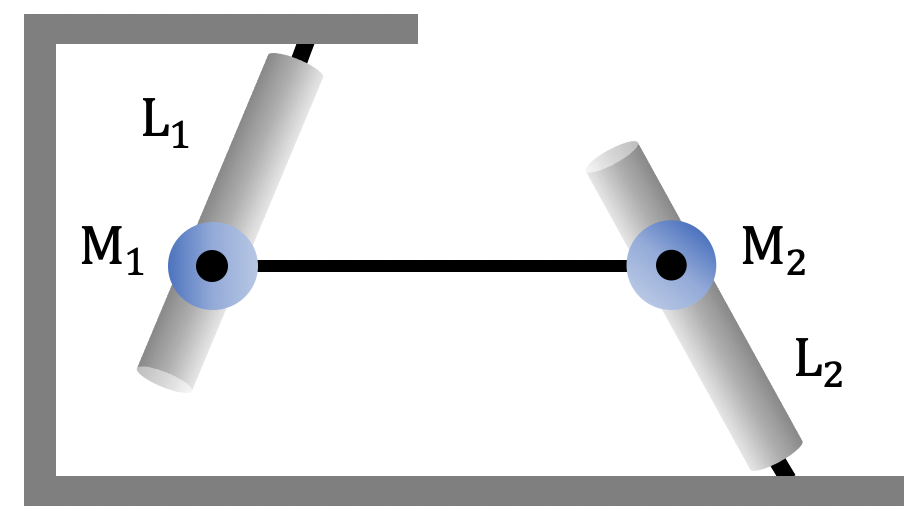
\includegraphics[width=120mm]{fig4_7.png} 
\caption[FP加速度計]{FP加速度計の概念図}
\label{fig4.7}
\end{center}
\end{figure}
\noindent
で与えられる($\gamma$はフレックスジョイントの剛性による影響を表す)\cite{39}. この共振周波数は, 2本のアームに対する重心位置を調節することで任意に下げることができる. \\
\quad KAGRAで用いるFP加速度計は幅140 mm, 高さ134 mm, 奥行き40 mmの大きさであり, IPの上にインストールすることができる. また, 真空中でも問題なく動作することも示されている\cite{FP}. 
\subsubsection{コイルマグネットアクチュエータ}
\label{sec4.1.2.4}
\vskip3mm
KAGRAのような重力波検出器では懸架された物体に力を加えるため, 真空で使える非接触のアクチュエータが必要になる. そこで永久双極子磁石とソレノイドコイルからなるコイルマグネットアクチュエータを用いる. これは永久磁石の静磁場とコイルに流れる電流の相互作用で発生する電磁気の力を利用したものであり, 十分な線形領域と作動力のダイナミックレンジを持つように設計されている. また, KAGRAの懸架系におけるコイルマグネットアクチュエータにはボイスコイル型と同軸可動磁石型の2種類があり\cite{41}, IPとGASには前者が, BFと低温懸架系には後者が用いられている. \\
\quad ボイスコイル型のアクチュエータは, 静磁場中を移動することでコイル内の電流がローレンツ力を受けるという作動原理である. 基準フレームに固定されている永久磁石(高透磁率の鉄製ヨークで成形されたもの)による一様な磁界の中にコイルのリード線が置かれ, ローレンツ力がコイル自身の作動力となる. \\
\quad 一方, 同軸可動磁石型のアクチュエータは永久磁石とソレノイドコイルが同軸に配置されており, 基準フレームに取り付けられたコイルの誘導磁界によって磁石に電磁力が加わる. 作動力の磁石の位置に対する依存性を軽減するために, 磁石はコイルの誘導磁界が十分均一である領域に配置されている. \\
\quad これらのアクチュエータでは常に最大作動力と雑音とのトレードオフがある. 大きな作動力を持つアクチュエータは, わずかな電気的変動でも雑音を生む. 特に防振懸架系の場合, 鏡に近いアクチュエータほど干渉計の感度に大きな影響を与える. そこで, KAGRAでは作動力とノイズの要件に応じて, 電流源と出力抵抗のオペアンプが異なる3種類のコイルドライバを使用している. Towerで用いられているものは表\ref{table4.3}に示した通りである. 
\begin{table}[H]
 \centering
  \begin{tabular}{ccccc}
   \hline\hline
   場所        & コイルドライバ & オペアンプ & 出力抵抗  & 最大電流 \\
   \hline
   IP・GAS・BF & ハイパワー     & OPA548     & 80 $\Omega$ & 0.12 A \\
   \hline
  \end{tabular}
 \caption[コイルドライバ(Tower)]{Towerで用いられているコイルドライバ. コイルのインピーダンスは出力抵抗には含まれていない. }
 \label{table4.3}
\end{table}

\section{低温懸架装置 (Cryogenic Payload)}
\subsection{機構}
BF以下は低温懸架系 (Cryogenic Payload) と呼ばれ, プラットフォーム(PF)から始まる. PFからはテストマス(TM)チェーンとリコイルマス(RM)チェーンの 2 つの3段振り子が並列に吊り下げられている. TMチェーンには上から順にマリオネット(MN), 中間マス(IM), テストマス(TM)という3つのステージがあり, RMチェーンはTMチェーンの対応するマスを取り囲むようなステージで, 地面の擾乱から隔離された作動力を加えることができる. 
\subsubsection{PF}
\vskip3mm
PFは低温懸架系の最上段にある円盤状のステージで, 長さ3.3 mのマルエージングワイヤでTower部分 (BF) と繋がっている(図\ref{fig4.8}左). PFには約4 Hzの共振周波数を持つベリリウム銅製の板バネが3枚取り付けられており, V方向の防振を行う. なお, TMチェーンはこの3枚の板バネが交わる点から吊るされている. また, PFからはRMチェーンがTMチェーンに並列に懸架されており, その回転を行うためのムービングマスがインストールされている(図\ref{fig4.8}右). 
\begin{figure}[H]
\begin{center}
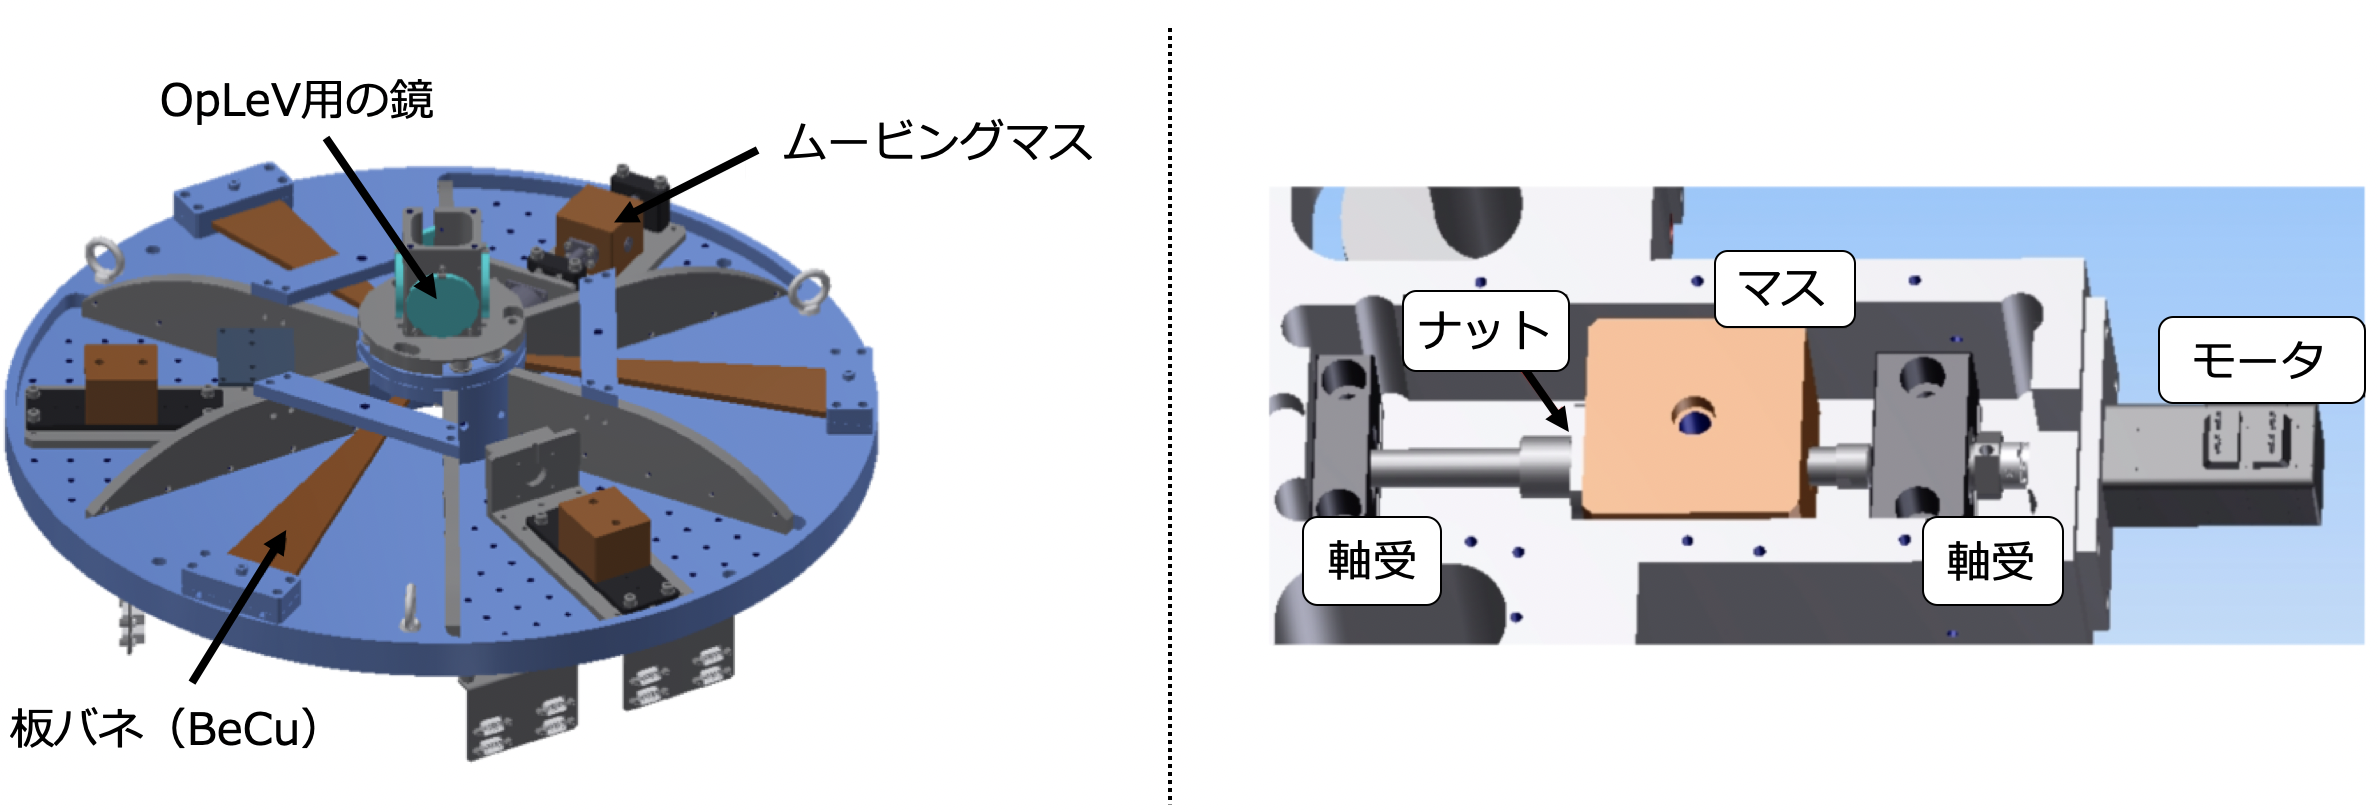
\includegraphics[width=150mm]{fig4_8.png} 
\caption[プラットフォーム (PF)とボールネジ型ムービングマス]{プラットフォーム (PF)とボールネジ型ムービングマス(ボールネジを用いてマスを動かす機構を持つ. ボールネジのナットがマスについているため, ネジの軸がモータによって回転するとマスがナットと共に動く. )\cite{42}}
\label{fig4.8}
\end{center}
\end{figure}
\subsubsection{MN}
\vskip3mm
マリオネット(MN)はTMチェーン初段の十字型ステージ(図\ref{fig4.9}左)であり, 回転自由度の剛性を低くするために質量中心に近い箇所を1本のマレージングワイヤで支持している. 干渉計の腕に沿った方向のMNの腕にはロープウェイ型ムービングマス(図\ref{fig4.9}右)が取り付けられており, MNの重心を変えることでTMのP方向の傾きを調節できる. なお, ボールネジ型のものを使用しないのは極低温かにおいて熱収縮によるスタックなど, ボールネジに起因する不具合が生じたからである\cite{42}. また, MNの下部にはOpLeV用の鏡があり, 外部からレーザーを当てることで, 地面に対するMNの角度をモニターすることができる(\ref{sec4.2.2.1}節および補遺\ref{補遺B}参照)\\
\quad 一方, マリオネットリコイルマス(MNR)はMNを囲むように取り付けられている(相対距離の初期値:20 mm). これは先述の通り3本のワイヤで懸架されているため, 1本のワイヤで吊られたMNに比べてY方向に揺れにくい. そこでMNRに設置されたフォトセンサによってMNとの相対位置を測定し, その信号をコイルマグネットアクチュエータ(MNに磁石・MNRにコイルがつけられている)にフィードバックすることによってダンピング制御を行っている(\ref{sec4.2.2.2}節および第\ref{第6章}章参照). 
\begin{figure}[H]
\begin{center}
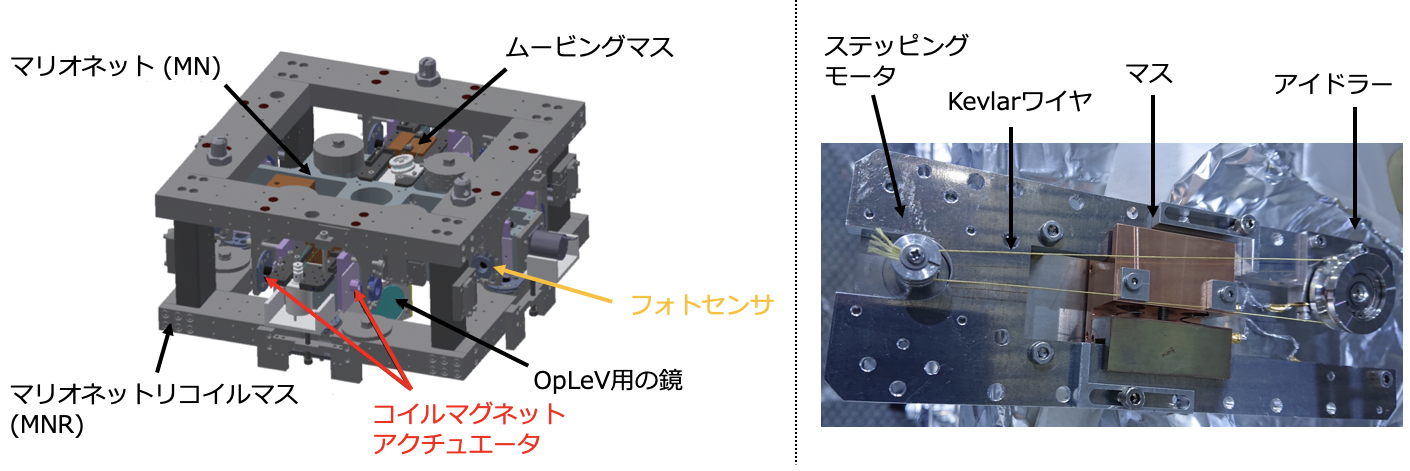
\includegraphics[width=180mm]{fig4_9.png}
\caption[マリオネット (MN)とマリオネットリコイルマス(MNR), およびロープウェイ型ムービングマス]{マリオネット (MN)とマリオネットリコイルマス(MNR), およびロープウェイ型ムービングマス(マス・Kevlarワイヤ・ステッピングモータ・アイドラーで構成されており, ワイヤとモータでマスを引っ張ることでMNの重心を変えている)\cite{42}}
\label{fig4.9}
\end{center}
\end{figure}
\subsubsection{IM}
\vskip3mm
中間マス(IM)はMNからベリリウム銅製のワイヤ4本で吊られている(図\ref{fig4.10}). IMにはサファイアブレード(サファイアファイバーを懸架するサファイア製の板バネで, ファイバーの縦方向の共振周波数を下げるほか, 長さのばらつきを補正する役割を持つ. )が取り付けられており, ミラーのV方向の防振を行っている. \\
\quad 中間リコイルマス(IRM)はMNRと同様, IMを囲むように取り付けられている(相対距離の初期値:20 mm). フォトセンサやコイルマグネットアクチュエータについてもMNRと同様で, MN段で制御できない固有モードも制御している. 
\begin{figure}[H]
\begin{center}
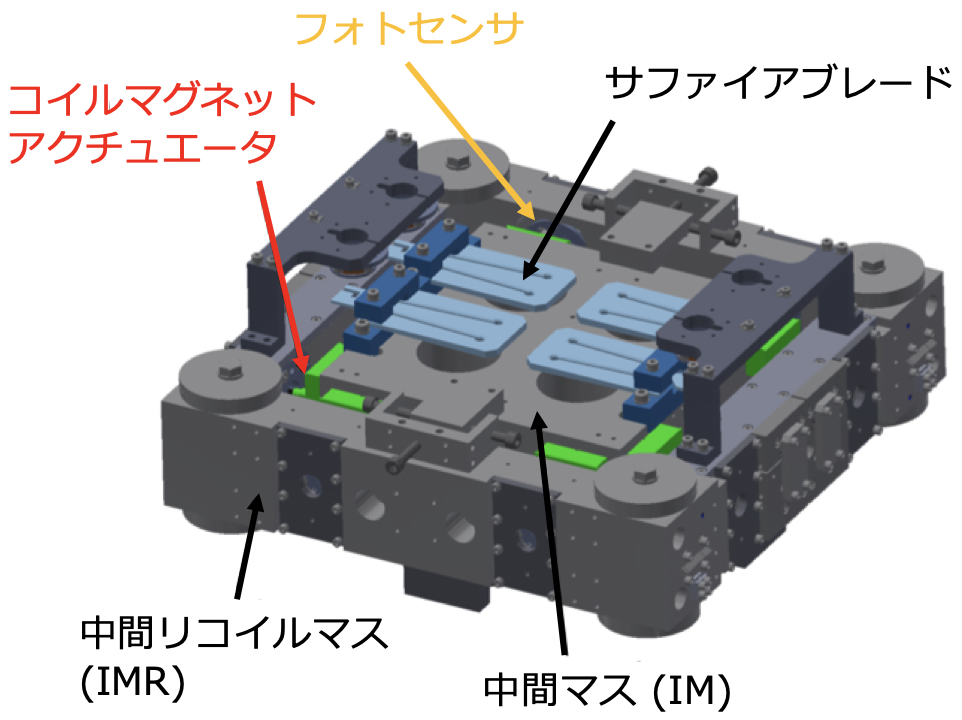
\includegraphics[width=90mm]{fig4_10.png} 
\caption[中間マス(IM)と中間リコイルマス(IRM)]{中間マス(IM)と中間リコイルマス(IRM)}
\label{fig4.10}
\end{center}
\end{figure}
\subsubsection{TM}
\vskip3mm
テストマス(TM)はサファイア鏡(直径220 mm・厚さ150 mm・質量23 kgの円筒形)であり, 低温懸架系の最下段に位置する(図\ref{fig4.11}). この鏡は低い熱雑音と高い熱伝導率を持ち, レーザー波長での高反射率, 低吸収率を実現させるため誘電体多層膜コーティングを施されている. しかしTMには常にレーザーが照射されることで熱を吸収し, 温度が上がってしまうので熱雑音が大きくなる. そこで直径1.6 mmのサファイアファイバー(TMの基材と同じ材料)4本で懸架し, 熱伝導率を向上させている. なお, ファイバーを引っ掛けるためにTMの側面2箇所にフラットカットを入れ, スリットが入ったイヤーと呼ばれるプリズムがHCB(Hydroxide Catalysis Bonding \cite{43})で取り付けられている. また, TMにもMNと同様OpLevが用いられているが, 地面に対する角度をモニターする Angle-sensing OpLev に加えて, 鏡の光軸方向の揺れを見るためのLength-sensing OpLev も設置されている. \\
\quad リコイルマス(RM)についてはMNやIMと同じく, TMを覆うように吊られており, TM・RM間のコイルマグネットアクチュエータで3自由度(L, P, Y)を制御している. 
\begin{figure}[H]
\begin{center}
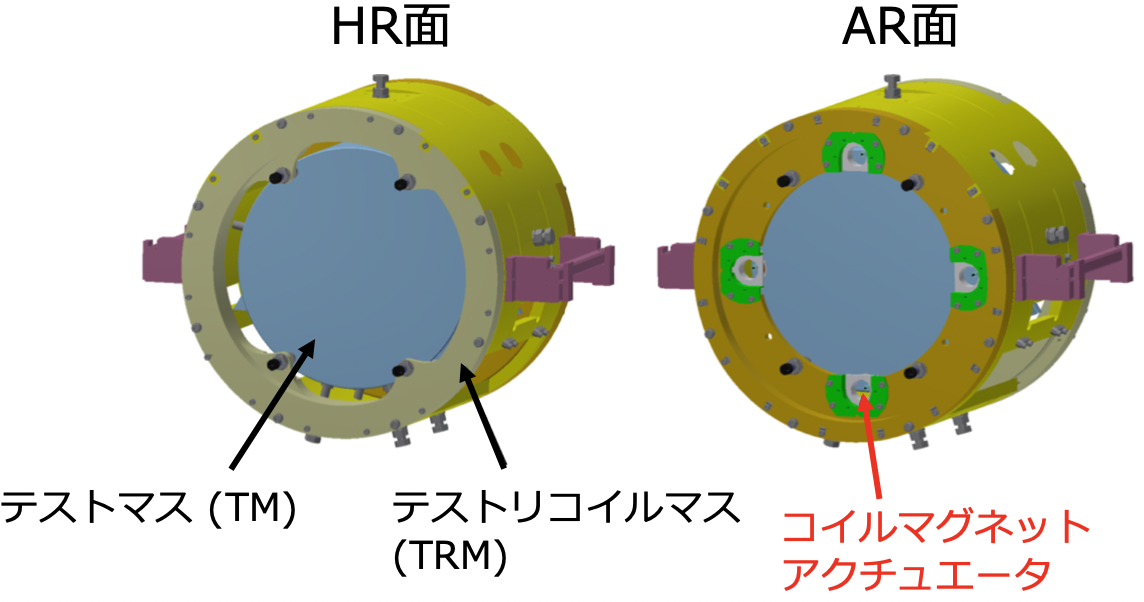
\includegraphics[width=130mm]{fig4_11.png} 
\caption[テストマス (TM)とそのリコイルマス (TMR)]{テストマス(TM)とそのリコイルマス(RM)}
\label{fig4.11}
\end{center}
\end{figure}
\subsection{センサ・アクチュエータ}
\label{sec4.2.2}
\vskip3mm
上述の通り低温懸架系の制御にはセンサとアクチュエータを用いる. MNとIMに関しては各自由度についてそれぞれフォトセンサでリコイルマスとの相対変位を測定できるようになっており, また, 地面に対する角度の測定はMNとTMに取り付けられた光てこを用いている. また, このアクチュエータで制御できる方向は図\ref{fig4.12}に示した通りで, MN・IMに関しては6自由度, 鏡に関してはL, P, Yの3自由度になっている. 以下ではそれぞれのセンサおよびアクチュエータについて簡単に記述する. 
\begin{figure}[H]
\begin{center}
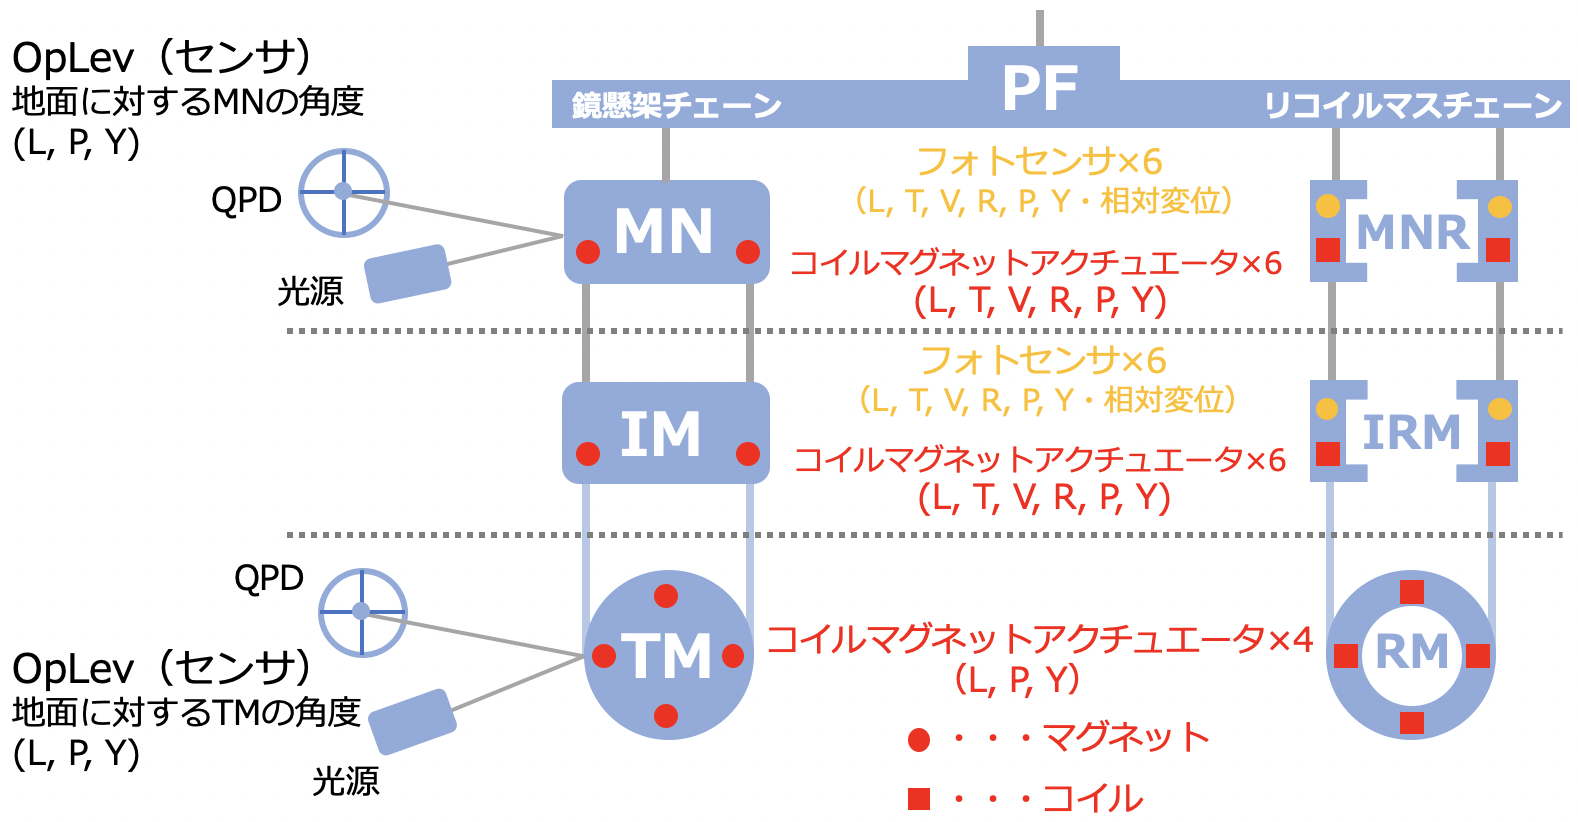
\includegraphics[width=160mm]{fig4_12.png} 
\caption[Payloadに関係のあるセンサ・アクチュエータ]{Payloadに関係のあるセンサ・アクチュエータ}
\label{fig4.12}
\end{center}
\end{figure}
\subsubsection{OpLev}
\label{sec4.2.2.1}
\vskip3mm
OpLevは鏡にレーザーを当てて, その反射光のビームスポットの位置を検知し, 鏡の地面に対する角度(水平)変位をモニターするものである. 低温懸架系ではMNにAngle sensing (角度方向の揺れを見る), TMにAngle sensingおよびLength sensing (水平方向の揺れを見る) OpLevを設置している. それらの原理については補遺\ref{補遺B}参照. また, 反射光の検知はQPD (Quadrant PhotoDiode) で行っている. 
\subsubsection{フォトセンサ}
\label{sec4.2.2.2}
\vskip3mm
センサには接触型のものと非接触型のものがある. 接触型センサは変位を高精度で読み取ることができるが, センサの振動がターゲットを揺らしてしまうので, KAGRAの懸架系に用いるのは不適切である. それに対し, 光や超音波を用いる非接触型センサは外乱を与える心配がない. \\
\quad そこで重力波検出器では非接触型のセンサを用いている. その中でも, 鏡を極低温まで冷却するKAGRAでは, 反射型のフォトセンサを用いている. これは反射型のフォトセンサがシャドーセンサ\footnote{マスの運動に伴ってフラッグがPDに入る光を遮る方向に動き, 光量の変化を変位として検出するセンサ. ダイナミックレンジが数 mmと小さいので冷却した際にフラッグがセンサに衝突して使用不可になる恐れがある. }などに比べてダイナミックレンジが広く, 冷却した際の熱収縮等でセンサが使えなくなる心配が少ないからである. \\
\quad 反射型フォトセンサはLEDおよび2つのPDから構成される. KAGRAではLED・PDを選定するための研究\cite{44}を行い,  Thorlabs社のInGaAs素子LED1200E\cite{45}をLED, InGaAsP製のFGA21\cite{46}をPDとして採用した. これはエネルギーバンドギャップの小さなInGaAsではエネルギーを媒介するキャリアとしてフォノンを使わない\footnote{フォノンは低温で励起しづらい. Siなどはエネルギーを運ぶキャリアがフォノンなので低温光学の分野では用いられない. }ので, 冷却した際も十分に動作できるからである. \\
\quad また, 反射型フォトセンサの動作原理は以下の通りである. LEDとPDは共にセンサに取り付けられており, LEDから出た光がターゲットで反射し, PDで検知される. このとき, 光軸方向のターゲット位置の変化に伴って反射光量も変化するので, そこからセンサ(リコイルマスチェーン側)とターゲット(鏡懸架チェーン側)の相対距離を割り出している(図\ref{fig4.13}右). 
\begin{figure}[H]
\begin{center}
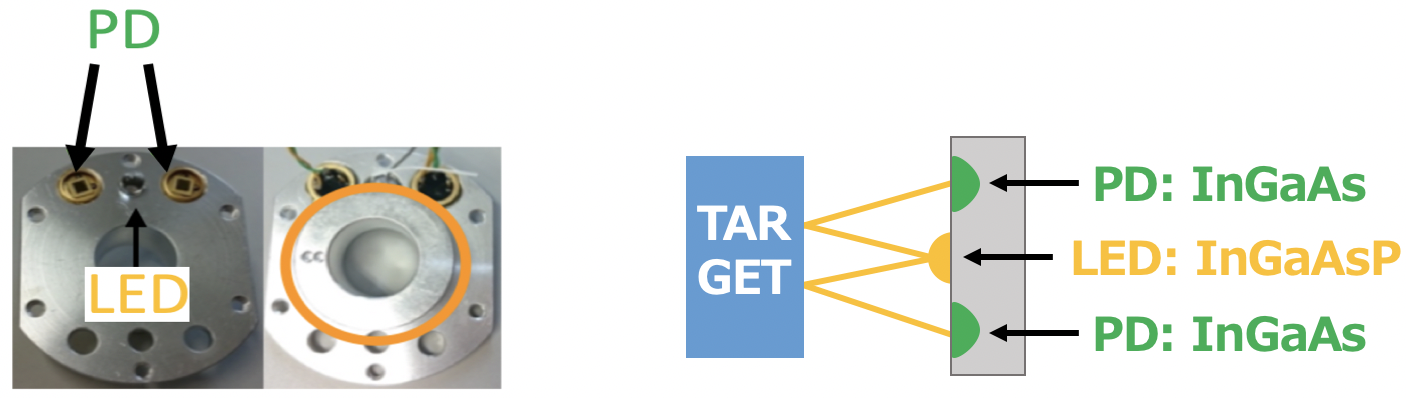
\includegraphics[width=170mm]{fig4_13.png} 
\caption[反射型フォトセンサとその動作原理]{実際にインストールされている反射型フォトセンサ(左)\cite{47}とその動作原理(右)}
\label{fig4.13}
\end{center}
\end{figure}
\subsubsection{コイルマグネットアクチュエータ}
\label{sec4.2.2.3}
\vskip3mm
低温懸架系で用いられるコイルマグネットアクチュエータは\ref{sec4.1.2.4}に示した通り, 同軸可動磁石型のものである. また, 低温懸架系の場合, 磁石がTMチェーンに, コイルがRMチェーンに取り付けられている. なお, 低温にしたときの特性の変化とバルクハウゼンノイズが小さいという理由でマグネットにはSmCo(サマリウムコバルト)を用いている. \\
\quad コイルドライバについては, 作動力とノイズのトレードオフを考慮し, MN・IMとTMで異なるものを使用している(表\ref{table4.4}). 
\begin{table}[H]
 \centering
  \begin{tabular}{ccccc}
   \hline\hline
   場所 & コイルドライバ & オペアンプ & 出力抵抗      & 最大電流 \\
   \hline
   MN   & ローパワー     & AD8671     & 1.4 k$\Omega$ & 9.5 mA \\
   IM   & ローパワー     & AD8671     & 1.4 k$\Omega$ & 9.5 mA \\
   TM   & ローパワー     & AD8671     & 7.8 k$\Omega$ & 1.3 mA \\
   \hline
  \end{tabular}
 \caption[コイルドライバ(低温懸架系)]{低温懸架系で用いられているコイルドライバ\cite{48}. コイルのインピーダンスは出力抵抗には含まれていない. }
 \label{table4.4}
\end{table}

\subsection{冷却システム}
低温懸架系は, 8 K innerシールドと80 K outerシールド\footnote{どちらもアルミニウム(Al1070)製で合わせて1400 kgある. また, 放射冷却をさらに向上させるため, innerシールドにはDLC(Diamond Like Coating)が施されている. }からなる二重構造のクライオスタットの中で, 4つの超低振動PTC(Pulse-Tube Cryocooler:パルス管冷凍機)を用いて冷却される(図\ref{fig4.14}). このPTCには2つの低温ステージ(それぞれ約40 Kと約4 Kに冷却する)があり, それぞれがVR(Vibration Reduction:振動減衰)ステージに熱的に接触している. また, PTC-1, 2, 3, 4の1段目はouterシールドに, PTC-2と4の2段目はinnerシールドに接続されている\cite{49}. 
\begin{figure}[H]
\begin{center}
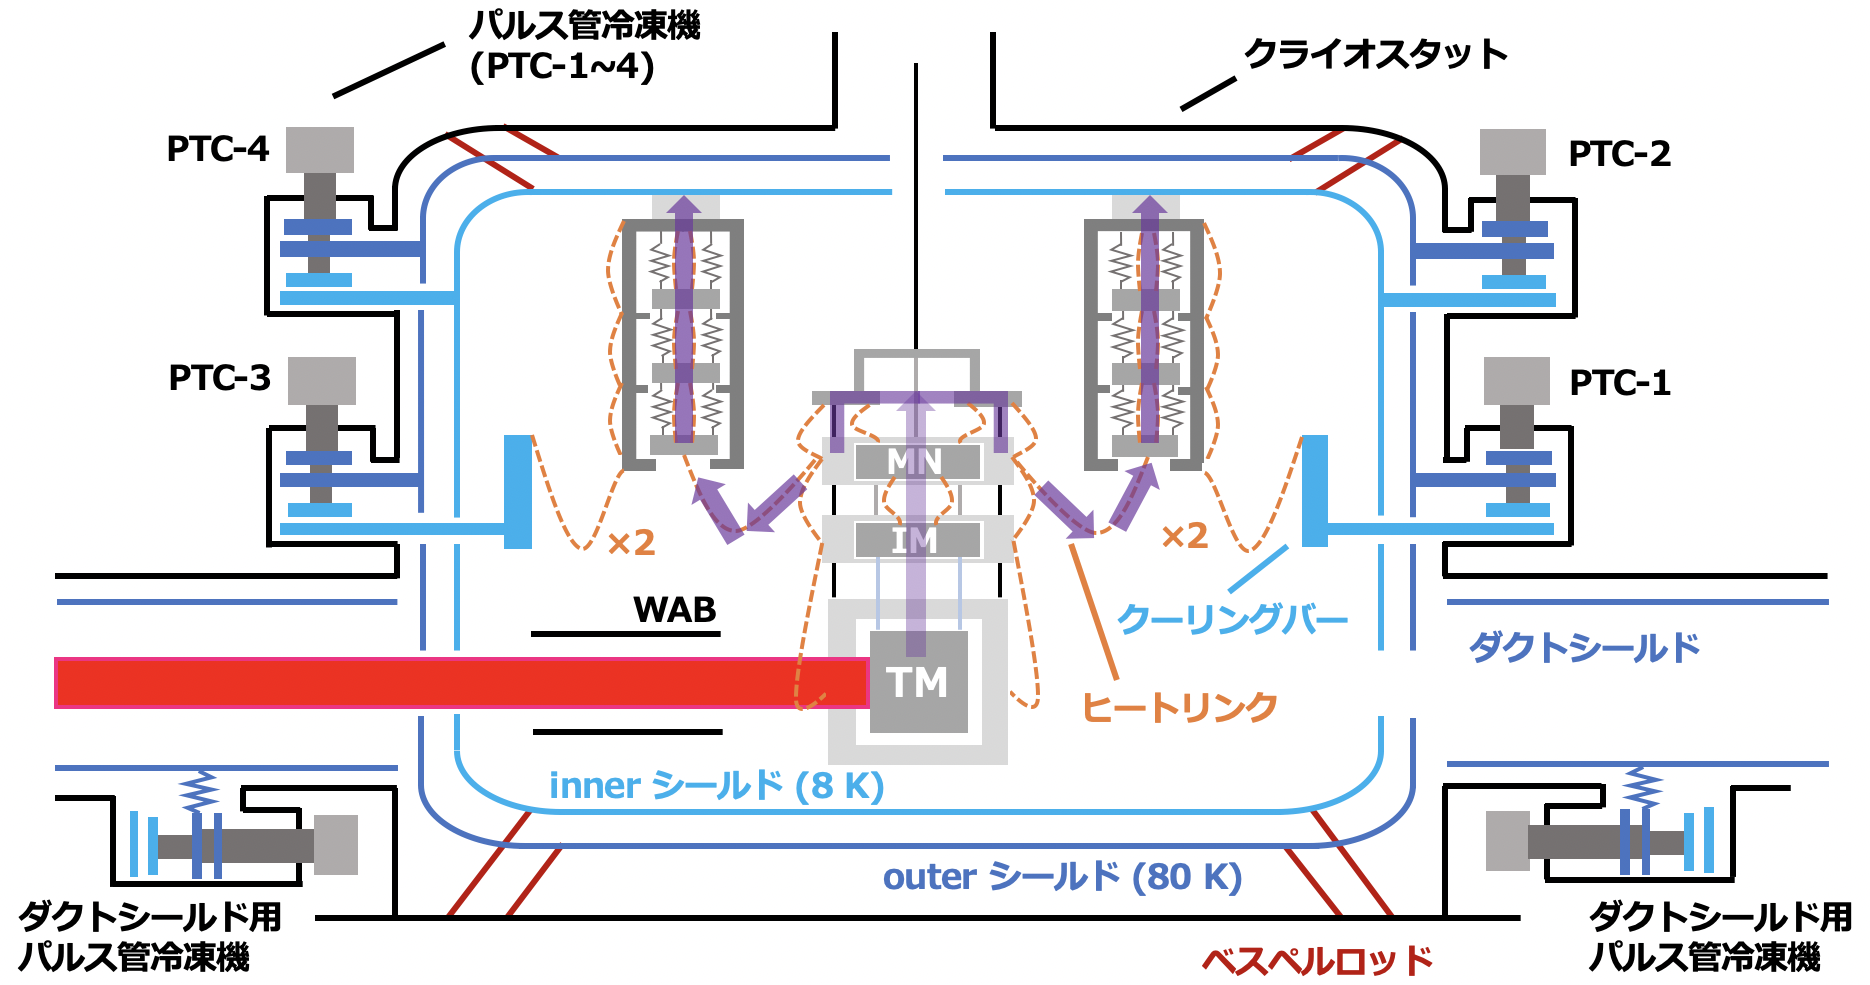
\includegraphics[width=170mm]{fig4_14.png} 
\caption[低温懸架系の冷却システム]{低温懸架系の冷却システム. 低温懸架系は二重放射シールドを持つクライオスタット内で冷却される. 1番外側の黒が逆真空容器, 内側の青は80Kと8Kの放射線シールドを示している. 80KシールドはPTC-1,2,3,4の1段目で冷却され, 8KシールドはPTC-2と4の2段目で冷却される. PTC-1と3の2段目はクーリングバーに接続され, 6N Al製のヒートリンクを通して低温懸架系を冷却する. また, クライオスタットの左右にあるダクトシールドは, 1段のPTCで120Kまで冷却される. }
\label{fig4.14}
\end{center}
\end{figure}
低温懸架装置の冷却における熱伝達経路は放射冷却と伝導冷却の2つに分けられる. まず放射冷却について, 先に示した二重の放射シールドは八角柱の構造で, 300 Kの外部放射から低温懸架装置を隔離して冷却する. このシールドからの熱放射により, 低温懸架装置は約100 Kまで効果的に冷却される. また, レーザーの光路を作るシールドの両脇の穴も熱放射源となる. この穴からの300 Kの放射を最小限にするため, 左右に5 mのダクトシールドが設置されており, それぞれのダクトシールドはダクトシールド用のPTCの1段目によって120 Kまで冷却される\cite{49}. \\
\quad 次に伝導冷却について, Payloadの各ステージはヒートリンクと呼ばれる6N (6 Nine, すなわち99.9999$\%$) のAlのケーブルで接続され, 伝導冷却が行われる\cite{50}. TMに吸収された熱は上段へ流れ, 最終的にヒートリンクとAl クーリングバーを通してクライオスタットへ抽出するという仕組みである. この機械的伝導経路は, 各ステージにさらなる振動を引き起こす可能性があるため, MNRに取り付けられたヒートリンクを中継する3段の防振系がクライオスタットに実装されている. この伝導冷却によって, TMの温度を20Kまで下げることができる. \\\\
\noindent
第\ref{第5章}章以降ではこのType-A Suspensionの内, 特に低温懸架系の特性評価および制御について記述する. 

\chapter{低温懸架装置の特性評価}
\label{第5章}
\fontsize{11pt}{16pt}\selectfont
この章では低温にした際, 懸架装置の特性がどのように変化するかということについて述べる. 
\section{特性評価の目的}
第\ref{第1章}章で述べた通りKAGRAでは鏡を極低温に冷却するが, これは2023年現在運転中の他の重力波検出器にはない大きな特徴である. しかし, 低温にすると鏡や懸架ワイヤなどの物性が変化することで共振周波数や伝達関数も変化する. すると, それに伴いかけるべき制御も変更する必要が生まれることがある. そこで低温にした際, ローカル制御に用いるフォトセンサの出力や懸架装置の伝達関数, Q値が室温と比較してどのように変化したかを調べた. \\
\quad なお, ETMY, ITMX, ITMYは2022年1月現在$250$ Kほどまでしか冷却されていないため, ETMXについてのみ, 特性評価を行った. \\
\quad また,  ETMXのMNの温度変化は図\ref{fig5.1}の通りであり, 277 Kから82 Kまで冷却された状態で特性評価を行った. 
\begin{figure}[H]
\begin{center}
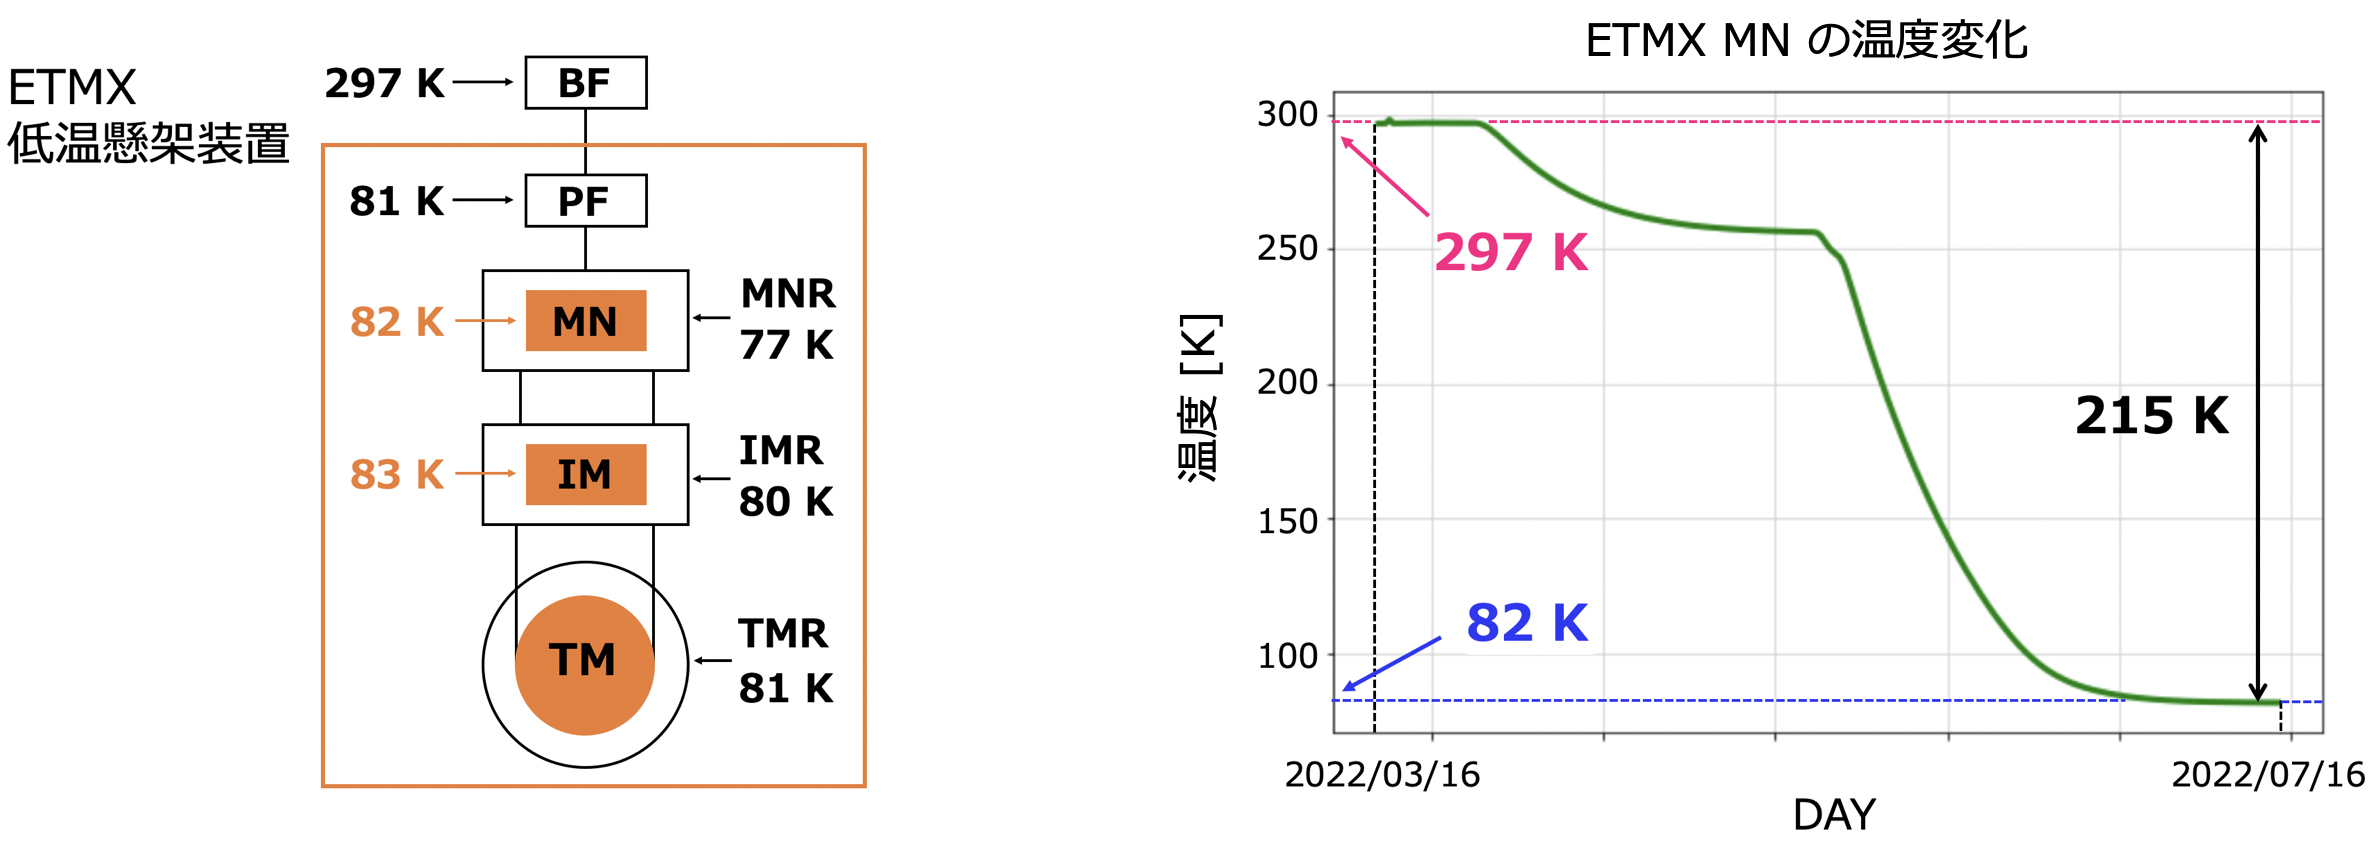
\includegraphics[width=170mm]{fig5_1.png}
\caption[ETMXの低温懸架装置の温度]{ETMXの低温懸架装置の温度(左)とETMX MNの温度変化(右)}
\label{fig5.1}
\end{center}
\end{figure}
\section{室温と低温下での特性の比較}
\subsection{フォトセンサの出力}
第4章で述べたように, 反射型のフォトセンサを用いてMN, IM段とそれぞれのリコイルマスとの距離を測定し, その信号を用いてローカルな制御を行っている.  ここではフォトセンサの出力が室温から低温への変化でどのように変化するか調べた. 
\subsubsection{測定結果}
\vskip3mm
MN, IM段で用いられるフォトセンサの出力を室温と低温下で比較したところ, 図\ref{fig5.2}, \ref{fig5.3}のようになった. これらの図では室温 (297 K) での出力を1とし, 他の温度ではそれに対して何倍の出力があるかということを示した. \\
\quad これより, 低温にするとフォトセンサの出力が増加するのが分かる. これは, 低温にすると小さな変化をより大きく見られることを示しており, またインストール前に\cite{47}で測定された結果と一致している.  \\\\
\begin{figure}[H]
\begin{center}
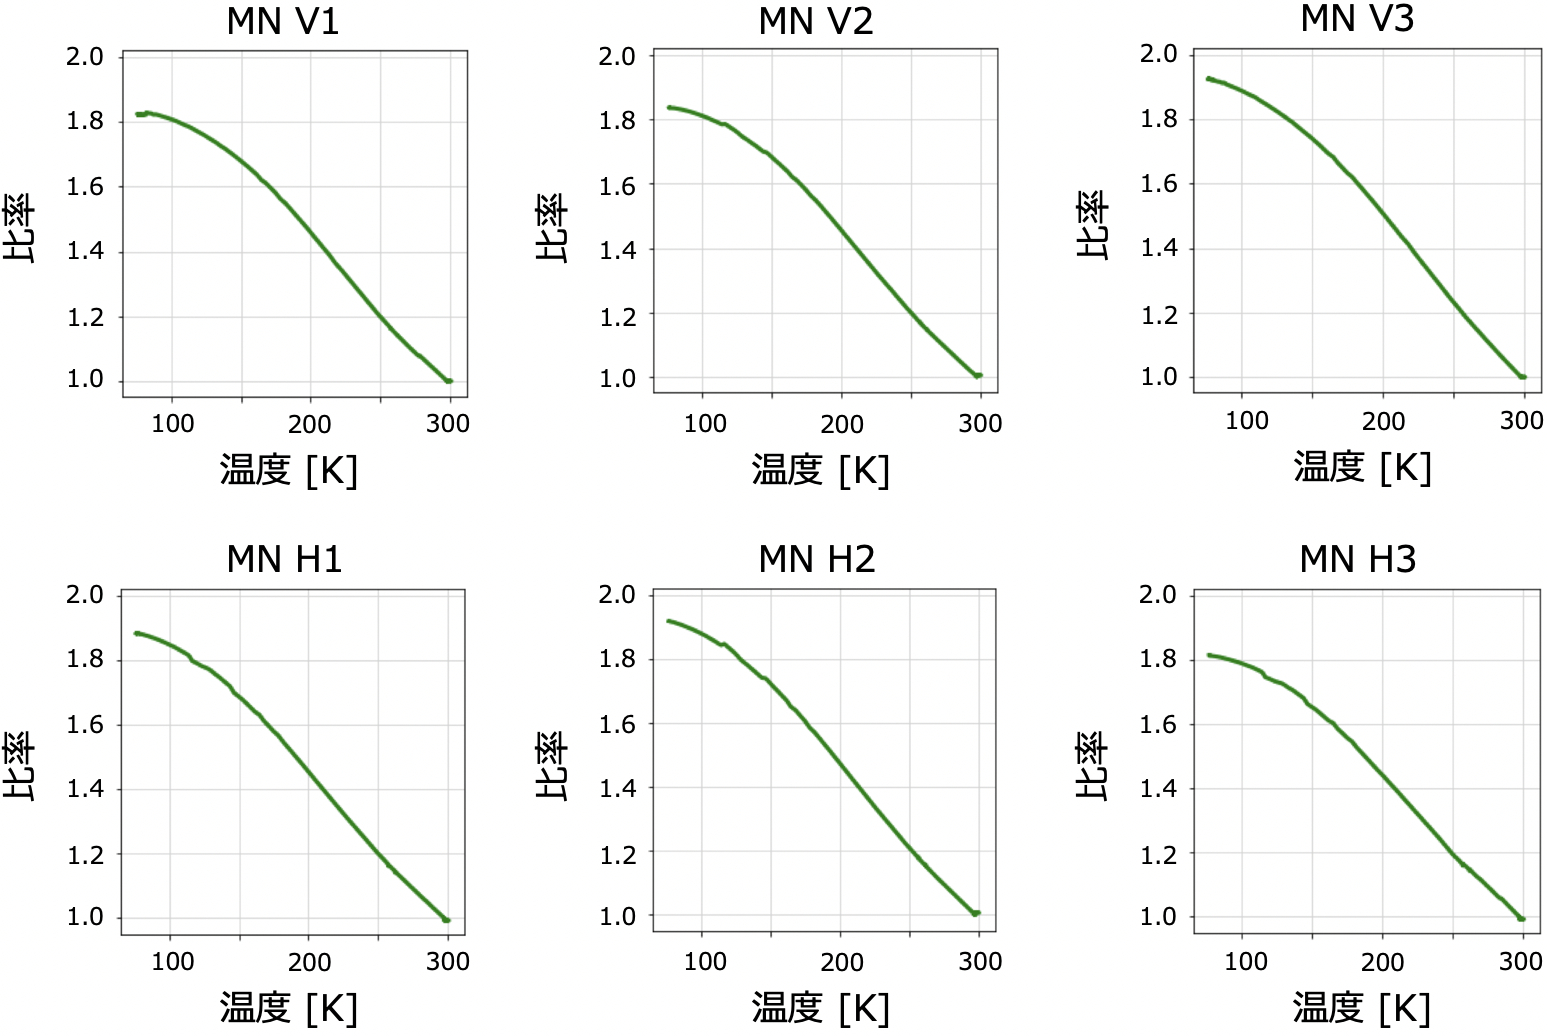
\includegraphics[width=160mm]{fig5_2.png}
\caption[フォトセンサの出力(ETMX MN)の変化]{フォトセンサの出力(ETMX MN)の変化}
\label{fig5.2}
\end{center}
\end{figure}
\begin{figure}[H]
\begin{center}
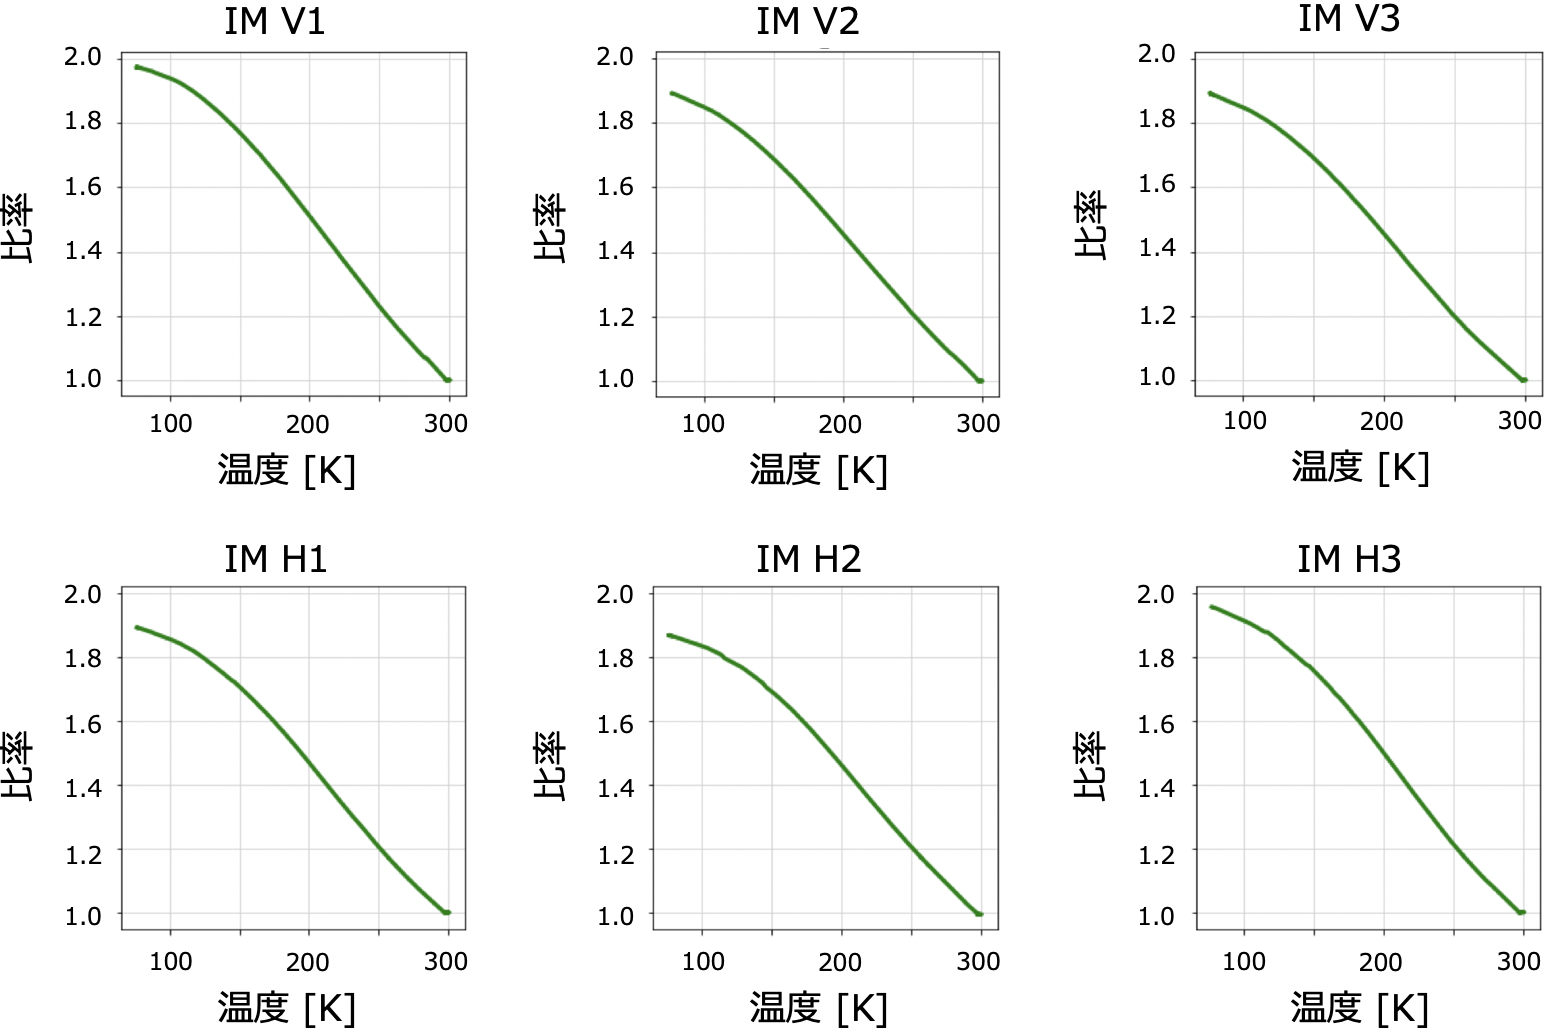
\includegraphics[width=160mm]{fig5_3.png}
\caption[フォトセンサの出力(ETMX IM)の変化]{フォトセンサの出力(ETMX MN)の変化}
\label{fig5.3}
\end{center}
\end{figure}
\begin{figure}[H]
\begin{center}
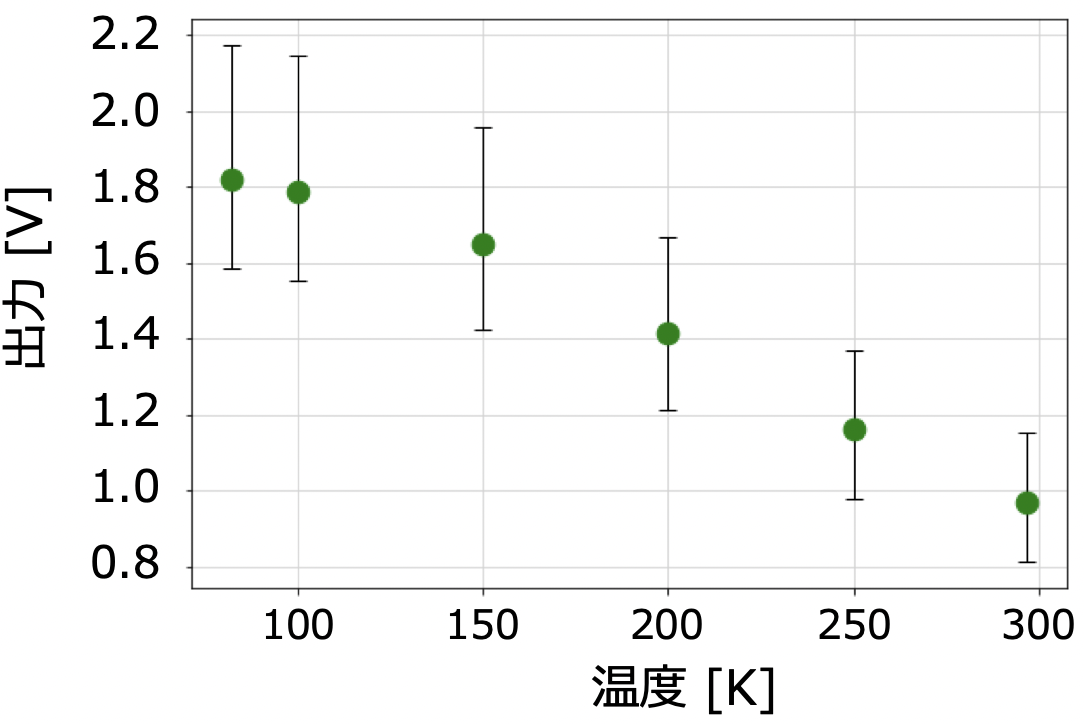
\includegraphics[width=140mm]{fig5_4.png}
\caption[温度ごとのフォトセンサの出力]{温度ごとのフォトセンサの出力の平均. エラーバーはそれぞれ出力の最小値, 最大値を表している.}
\label{fig5.4}
\end{center}
\end{figure}
\begin{table}[H]
 \centering
  \begin{tabular}{|c||c|c|c|c|}
   \hline
    温度& 平均値 & 標準偏差 & 最大最小の差  \\
   \hline
   297 K & 0.9662 V & 0.1021 V & 0.3389 V\\
   \hline
   250 K    &  1.163 V & 0.1219 V & 0.3907 V\\
   \hline
   200 K    & 1.414 V & 0.1494 V & 0.4559 V\\
   \hline
   150 K    & 1.648 V & 0.1775 V & 0.5310 V\\
   \hline
    100 K    & 1.789 V & 0.1906 V & 0.5904 V\\
   \hline
    82 K    & 1.822 V & 0.2044 V & 0.5915 V\\
   \hline
  \end{tabular}
 \caption[フォトセンサの出力の平均値およびばらつき]{フォトセンサの出力の平均値およびばらつき}
 \label{table5.1}
\end{table}
また, 図\ref{fig5.4}に示したのは各温度における12個のフォトセンサの出力の平均である.  なお, エラーバーはそれぞれ出力の最小値, 最大値を表している. さらに, 各温度における出力の平均値および標準偏差は表\ref{table5.1}の通りであり, これらより低温にすると出力のばらつきが大きくなるのが分かる.
\subsubsection{考察}
\vskip3mm
\cite{47}によると, センサの個体差が50\%以下であるという要求がある. これはキャリブレーションファクターの大きさが50\%以上変化すると, センサとターゲットの距離が$\pm 1$ cmという線形応答範囲にあるかどうか分からなくなるからである. 本研究において, 実際にKAGRAへインストールして冷却された状態で出力のばらつきを測定した結果, センサの個体差は82 Kにおいても平均値に対して32\%であり, 50\%以下という要求を満たすことが分かった. しかし, 低温にすると出力のばらつきは大きくなっており, 冷却が進むにつれてセンサの個体差がさらに広がる恐れがある. したがって, 今後さらに冷却する場合, フォトセンサの出力のばらつきに注意する必要がある.\\
\quad 補遺\ref{補遺C}に示したように, 反射型フォトセンサの出力はLEDのビームプロファイルに大きく影響を受ける. よってフォトセンサの出力のばらつきの原因としてLEDのビームプロファイルの違いが挙げられる. しかし, 低温でそのばらつきが大きくなる理由は説明できない. KAGRAの反射型フォトセンサに用いられるLEDの発光効率の個体差および温度との関係については, 今後調査する必要がある.

\subsection{共振周波数・伝達関数}
\subsubsection{測定結果}
\vskip3mm
MN段の各自由度方向 (L, P, Y) に励起信号を入れて振動させ, フォトセンサの出力で読み取ったMN段の各方向の動きまでの伝達関数を測定した. その結果を図\ref{fig5.5}, \ref{fig5.6}, \ref{fig5.7}に示す. これらより, 低温にすると共振周波数が数\%高くなっているのが分かる.
\begin{figure}[H]
\begin{center}
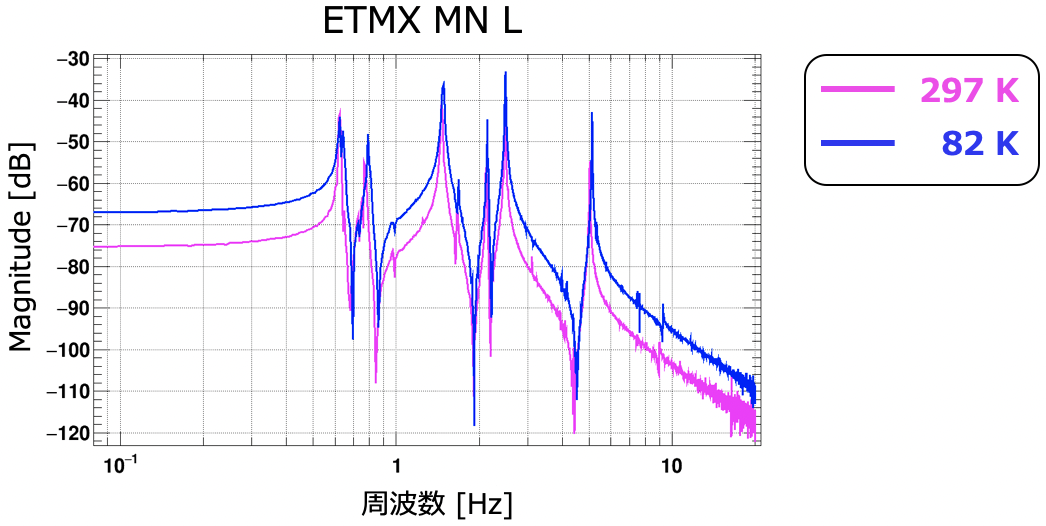
\includegraphics[width=150mm]{fig5_5.png}
\caption[室温と低温での伝達関数の比較 (L)]{室温と低温での伝達関数の比較(ETMXのMNのL). ピンク, 青の線がそれぞれ室温 (297 K) , 低温 (82 K) における伝達関数を示している.  }
\label{fig5.5}
\end{center}
\end{figure}
\begin{figure}[H]
\begin{center}
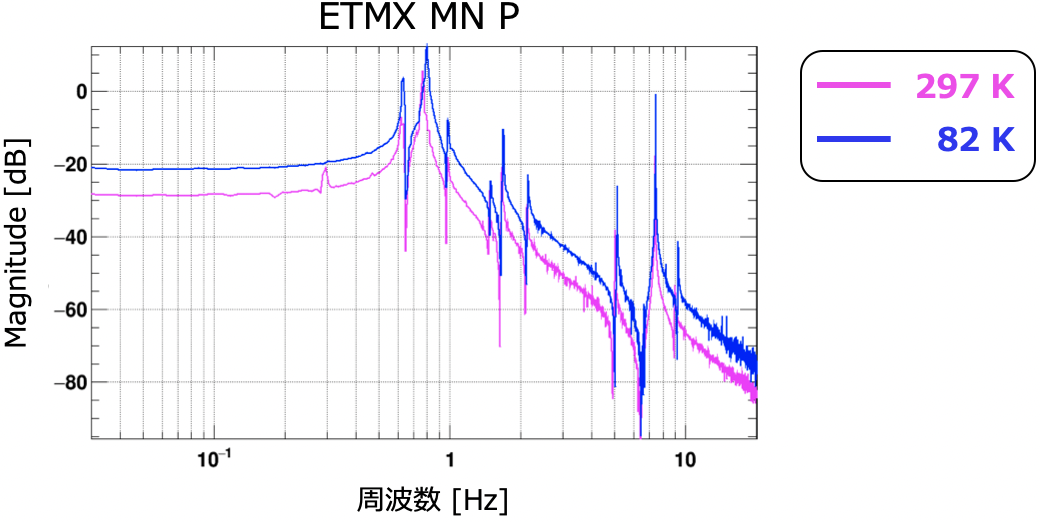
\includegraphics[width=150mm]{fig5_6.png}
\caption[室温と低温での伝達関数の比較 (P)]{室温と低温での伝達関数の比較(ETMXのMNのP). ピンク, 青の線がそれぞれ室温 (297 K) , 低温 (82 K) における伝達関数を示している.  }
\label{fig5.6}
\end{center}
\end{figure}
\begin{figure}[H]
\begin{center}
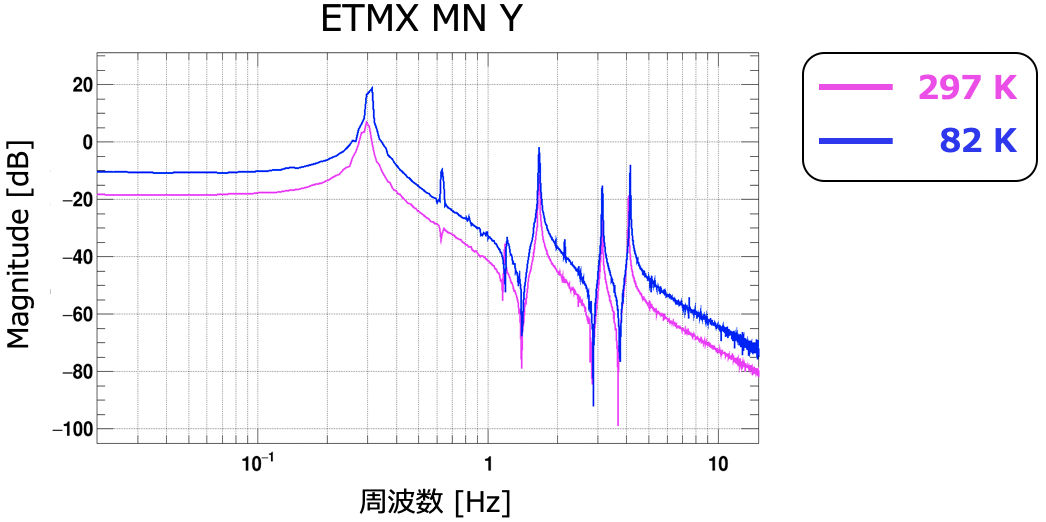
\includegraphics[width=150mm]{fig5_7.png}
\caption[室温と低温での伝達関数の比較 (Y)]{室温と低温での伝達関数の比較(ETMXのMNのY). ピンク, 青の線がそれぞれ室温 (297 K) , 低温 (82 K) における伝達関数を示している. }
\label{fig5.7}
\end{center}
\end{figure}
\begin{table}[H]
 \centering
  \begin{tabular}{|c||c|c|c|c|}
   \hline
    \diagbox{温度}{Mode}& 1 & 2 & 3 & 4 \\
   \hline
   297 K & 0.63 Hz & 1.46 Hz & 2.12 Hz & 2.47 Hz \\
   \hline
   82 K    & 0.63 Hz & 1.48 Hz & 2.13 Hz & 2.48 Hz \\
   \hline
  \end{tabular}
 \caption[共振周波数 (ETMX MN L)]{共振周波数 (ETMX MN L)}
\end{table}
\begin{table}[H]
 \centering
  \begin{tabular}{|c||c|c|c|c|}
   \hline
    \diagbox{温度}{Mode}& 1 & 2  \\
   \hline
   297 K & 0.76 Hz & 7.42 Hz  \\
   \hline
   82 K    & 0.80 Hz & 7.46 Hz \\
   \hline
  \end{tabular}
 \caption[共振周波数 (ETMX MN P)]{共振周波数 (ETMX MN P)}
\end{table}
\begin{table}[H]
 \centering
  \begin{tabular}{|c||c|c|c|c|}
   \hline
    \diagbox{温度}{Mode}& 1 & 2 & 3 & 4 \\
   \hline
   297 K & 0.29 Hz & 1.66 Hz & 3.13 Hz & 4.08 Hz \\
   \hline
   82 K    & 0.31 Hz & 1.67 Hz & 3.14 Hz & 4.16Hz \\
   \hline
  \end{tabular}
 \caption[共振周波数 (ETMX MN Y)]{共振周波数 (ETMX MN Y)}
\end{table} 
\subsubsection{考察}
\vskip3mm
一般に, 低温にするとヤング率が上昇することで共振周波数が増加すると考えられ, 予想通りの結果が得られたといえる. \\
\quad また, 励起信号からMNの動きまでの伝達関数のゲインが上がっているが, これはフォトセンサの出力が増加したことに由来する. フォトセンサの出力を各方向の変異に換算しているが, 冷却に伴いセンサの出力が増加した分を校正していないため伝達関数のゲインが上がっているのである.
\subsection{機械的Q値}
%機械的Q値(以下Q値と記述する)は共振の鋭さを表すパラメータであり, この値が大きいほど振動のエネルギーは共振のピークに押し込められる. これは共振周波数以外でのエネルギーが下がるということを意味しており, ゆえにQ値は熱雑音低減のために重要な値である. 
\subsubsection{測定方法}
\vskip3mm
Q値は伝達関数から求めることができる. 例えば減衰を含む調和振動子の運動方程式は
\begin{equation}
m\ddot{x}+m\omega_0^2x=f(t),
\label{eq5.1}
\end{equation}
と書けるが, これをFourier変換した上で散逸を表す項$\phi(\omega)$を付け加えると
\begin{equation}
-m\omega^2\tilde{x}+m\omega_0^2\left[1+i\phi(\omega)\right]\tilde{x}=\tilde{f},
\end{equation}
となる. なお, この$\phi(\omega)$を用いると位置および復元力は周波数領域において
\begin{equation}
\tilde{F}=-m\omega_0^2\left[1+i\phi(\omega)\right]\tilde{x},
\end{equation}
と書ける. つまり, 復元力の位相は位置の位相に対して$\phi$遅れる. ここで, 復元力が1周期の間にする仕事(復元力による仕事率$F\dot{x}$を1周期で積分したもの)を計算し, 系の全エネルギーで規格化すると$-2\pi\phi$となる. これが散逸したエネルギーであり, $\phi(\omega)$が散逸を示す項であることが分かる. \\
\quad ここで
\begin{equation}
\phi(\omega_0)=\frac{1}{Q},
\end{equation}
となる$Q$が機械的Q値である.\\
\quad この調和振動子の伝達関数の絶対値の2乗は
\begin{equation}
\left|H(\omega)\right|^2=\frac{1}{m^2\left\{(\omega^2-\omega_0^2)^2+w_0^4\phi^2(\omega)\right\}^2}.
\end{equation}
これは$\omega=\omega_0$のときにピークを持つが, その半値幅を$\Delta\omega_0$とすると
\begin{equation}
\left|H\left(\omega_0\pm\frac{\Delta\omega_0}{2}\right)\right|^2=\frac{\left|H(\omega_0)\right|^2}{2},
\end{equation}
でありピークの幅が小さいときは$\Delta\omega_0\ll\omega_0$であり, さらに$\phi(\omega)=\phi(\omega_0)=1/Q$と書けるので
\begin{equation}
\Delta\omega_0=\frac{\omega_0}{Q},
\label{eq5.7}
\end{equation}
となる. 式(\ref{eq5.7})から分かるように, Q値が低いほど半値幅$\Delta\omega_0$は大きくなる. よって伝達関数のピークの半値幅からQ値を求めるこの方法は, Q値が低い場合は有効である. \\
\quad しかし, 本研究における懸架系のQ値はある程度大きいため, 懸架系に外力を加えた時の減衰時間から求める手法をとる. 先ほどの調和振動子の式(\ref{eq5.1})において外力項を
\begin{equation}
f(t) = 
    \begin{cases}
        {A{\rm exp}(i\omega_0t) \quad (t<0)}\\
        {0 \quad\quad\quad \quad\quad\,\, (t>0)}
    \end{cases},
\end{equation}
とする. このとき, 運動方程式をFourier変換して$\tilde{x}$について解いた上で逆Fourier変換すると
\begin{equation}
x(t)\propto {\rm exp}\left(-\frac{\omega_0t}{2Q}\right).
\end{equation}
これより, 共振状態に励起した後で励起信号を切り, 振動の減衰時間を測定することでQ値を求めることができる. すなわち, 減衰の時定数を$\tau$としたとき
\begin{equation}
x(t)\propto {\rm exp}\left(-\frac{t}{\tau}\right),
\label{eq5.10}
\end{equation}
であるから$f_0=\frac{\omega_0}{2\pi}$を用いて
\begin{equation}
\tau=\frac{2Q}{\omega_0}=\frac{2Q}{2\pi f_0}=\frac{Q}{\pi f_0},
\end{equation}
となり, 
\begin{equation}
Q=\pi f_0\tau,
\label{eq5.12}
\end{equation}
と計算できる. \\
\quad 式(\ref{eq5.12})から分かる通りQ値が高いほど減衰時間が長く, フィッティングの精度が上がるため, 本研究の場合のような高いQ値の測定にはこの方法を用いる. \\
\quad 実際には, MN段に対応する共振周波数に等しい周波数の励起信号を入れた後でその励起を止め, 振動が減衰する時間を測定する. このとき, 減衰の様子は図\ref{fig5.8}に示す通りであり, Q値が大きいため振動が十分減衰するのに時間がかかるのが分かる. 減衰時間は式(\ref{eq5.10})で示したように減衰曲線の包絡線を指数関数でフィッティングすれば良い. 
%\footnote[100]{このままでは外乱があった際に干渉計が再ロックするまで長時間待たないといけないため, 次章に示すダンピング制御を行う. }
\begin{figure}[H]
\begin{center}
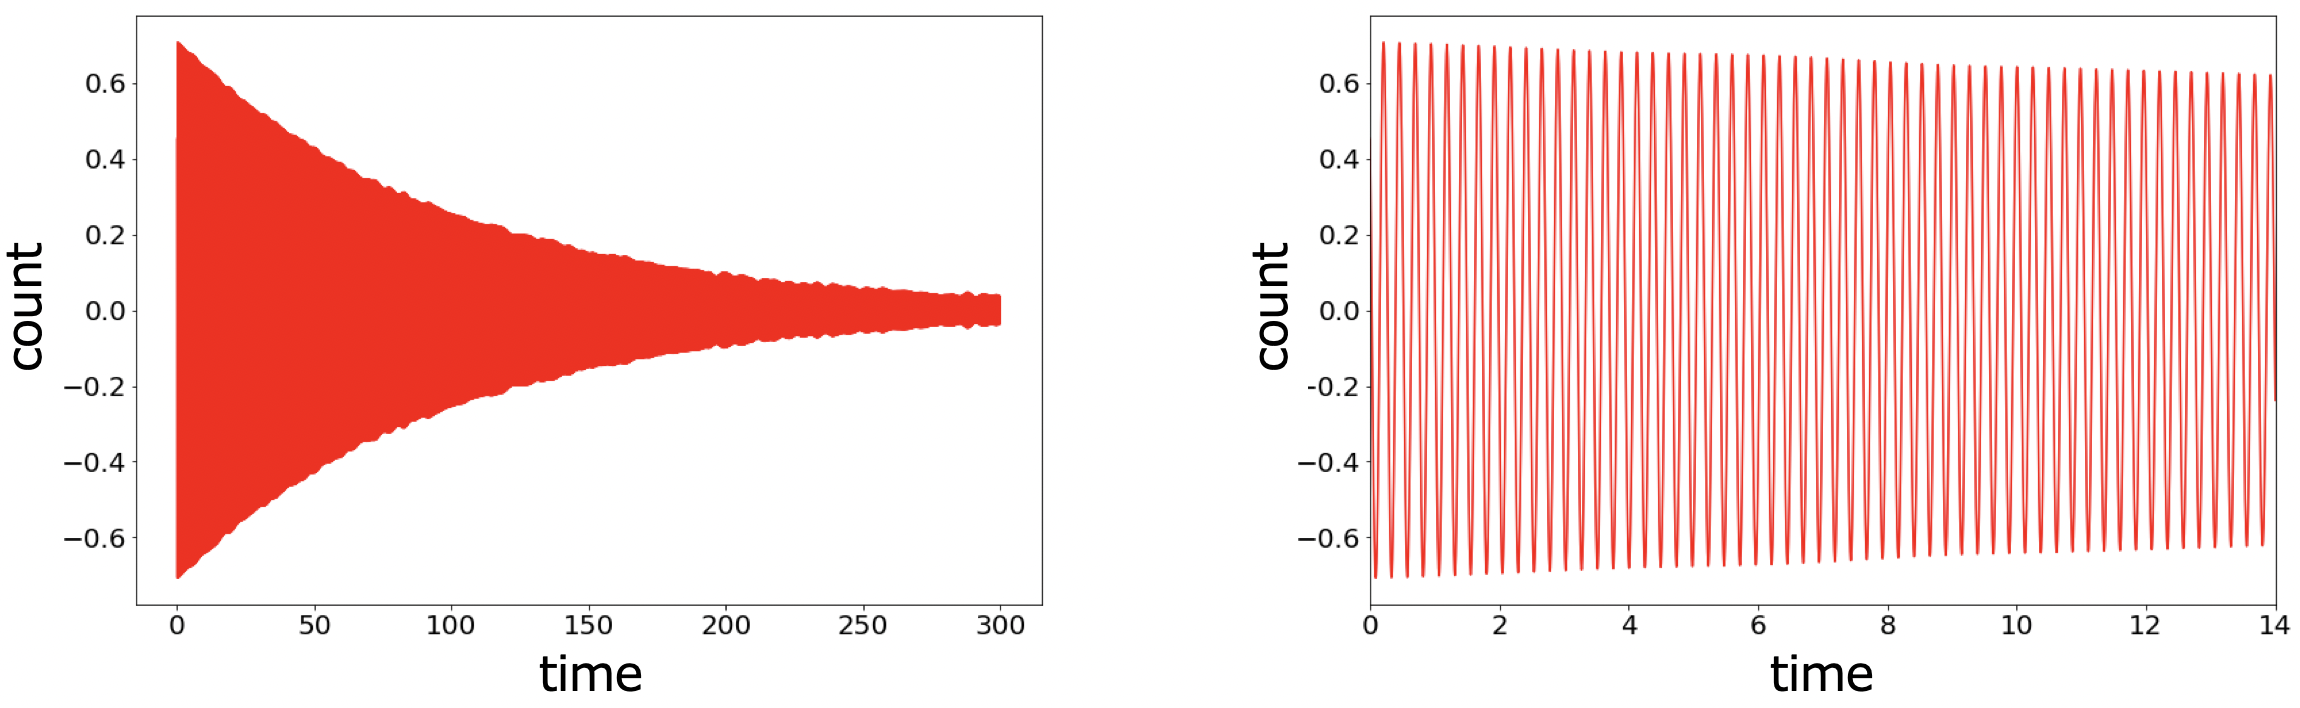
\includegraphics[width=170mm]{fig5_100.png}
\caption[励起信号を切った後の減衰の様子]{左図はETMXのMN段にY方向の励起信号 (4.08 Hz) を入れて共振状態にした後に励起信号を切ったとき, 振動が減衰する様子を示したものである. Q値が大きいため振動が十分減衰するまでは時間がかかる(右図は初めの約15秒間を拡大したものである). }
\label{fig5.8}
\end{center}
\end{figure}
\subsubsection{測定結果}
\vskip3mm
297 Kと82 KにおいてETMXのMNでQ値を測定した結果, L, P, Yのそれぞれの自由度に対する結果は表\ref{table5.5}, \ref{table5.6}, \ref{table5.7}のようになった. また, これを図示すると図\ref{fig5.9}のようになる. 
\begin{table}[H]
 \centering
  \begin{tabular}{|c||c|c|c|c|}
   \hline
    \diagbox{温度}{Mode}& 1 & 2 & 3 & 4 \\
   \hline 
   297 K & 1760.8 & 1251.7 & 2981.5 & 3160.4 \\
   \hline
   82 K    & 1504.0 & 1228.6 & 4245.6 & 1996.1 \\
   \hline
  \end{tabular}
 \caption[Q値 (ETMX MN L)]{Q値 (ETMX MN L)}
 \label{table5.5}
\end{table}
\begin{table}[H]
 \centering
  \begin{tabular}{|c||c|c|}
   \hline
    \diagbox{温度}{Mode}& 1 & 2  \\
   \hline 
   297 K & 435.47 & 3460.3 \\
   \hline
   82 K    & 440.38 & 9548.2 \\
   \hline
  \end{tabular}
 \caption[Q値 (ETMX MN P)]{Q値 (ETMX MN P)}
  \label{table5.6}
\end{table}
\begin{table}[H]
 \centering
  \begin{tabular}{|c||c|c|c|c|}
   \hline
    \diagbox{温度}{Mode}& 1 & 2 & 3 & 4 \\
   \hline
   297 K & 233.94 & 2603.5 & 4703.8 & 1245.2 \\
   \hline
   82 K    & 131.86 & 1789.9 & 5291.8 & 2287.2 \\
   \hline
  \end{tabular}
 \caption[Q値 (ETMX MN Y)]{Q値 (ETMX MN Y)}
  \label{table5.7}
\end{table}
\begin{figure}[H]
\begin{center}
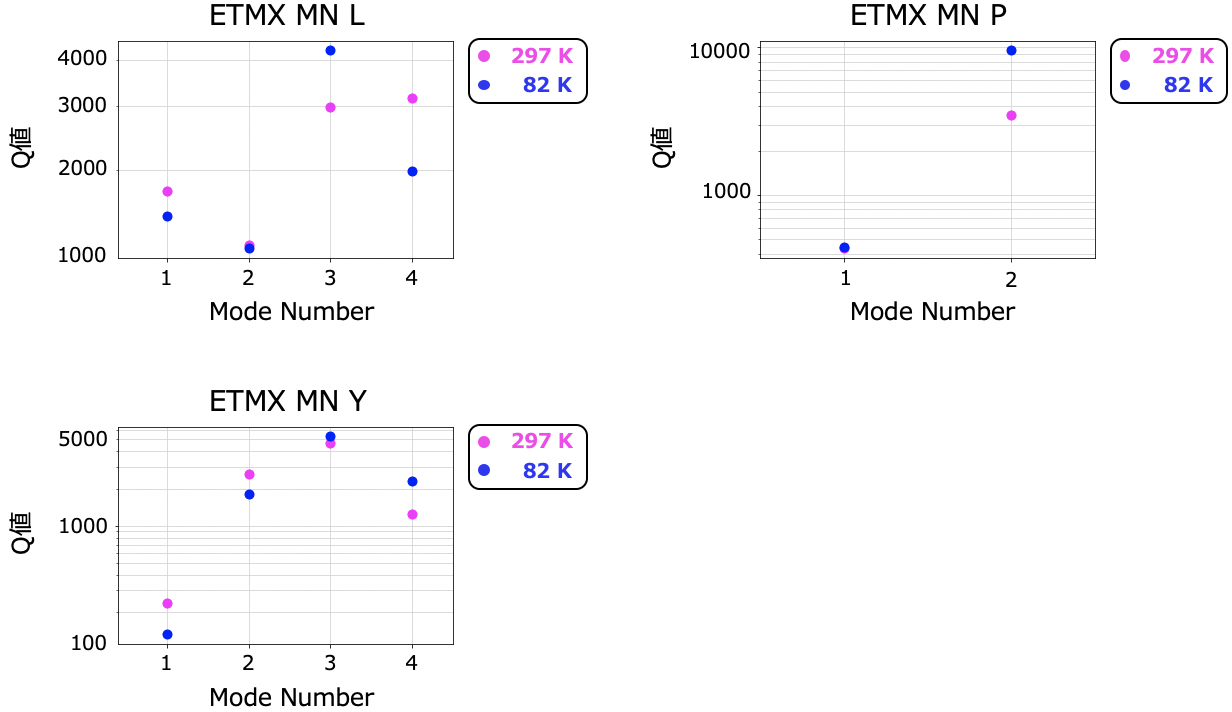
\includegraphics[width=170mm]{fig5_101.png}
\caption[室温と低温でのQ値の比較]{室温と低温でのQ値の比較(ETMXのMNのL,  P, Y). ピンク, 青の点がそれぞれ室温 (297 K) , 低温 (82 K) におけるQ値を示している. サファイアが低温においてQ値が高いという性質を持つため, 一般には, サファイアファイバーの影響が大きいモードでは低温にするとQ値が大きくなる. }
 \label{fig5.9}
\end{center}
\end{figure}
\subsubsection{考察}
\vskip3mm
%{\color{red}「サファイアが低温においてQ値が高いという性質を持つため, 一般には, サファイアファイバーの影響が大きいモードでは低温にするとQ値が大きくなる. 」という内容を書く. モードの説明・図示しながら. }
図5.7を見ると, Lの3つめのモード, Pの2つめのモード, Yの4つめのモードでは低温にした時にQ値が増加している.  これは2.2.4.2で述べたように, 低温で高いQ値を示すサファイアファイバーの影響を大きく受けるからであると考えられる. 実際, \cite{eigen}にまとめられたType-A suspensionの固有モードのリストによると, これらのモードはサファイアファイバー(低温懸架装置の下部)の影響を大きく受けるモードとなっており, 本研究で得られた結果と合致している.\\
\quad また, ダンピング制御に変更の必要性があるかどうかは第\ref{第6章}章に示す.


\newpage
 
\newpage
\chapter{ダンピング制御}
\label{第6章}
\fontsize{11pt}{16pt}\selectfont
この章ではダンピング制御について, その必要性と原理を説明した後, 実際の制御とその効果について記す. 
\section{ダンピング制御とその必要性}
\begin{figure}[H]
\begin{center}
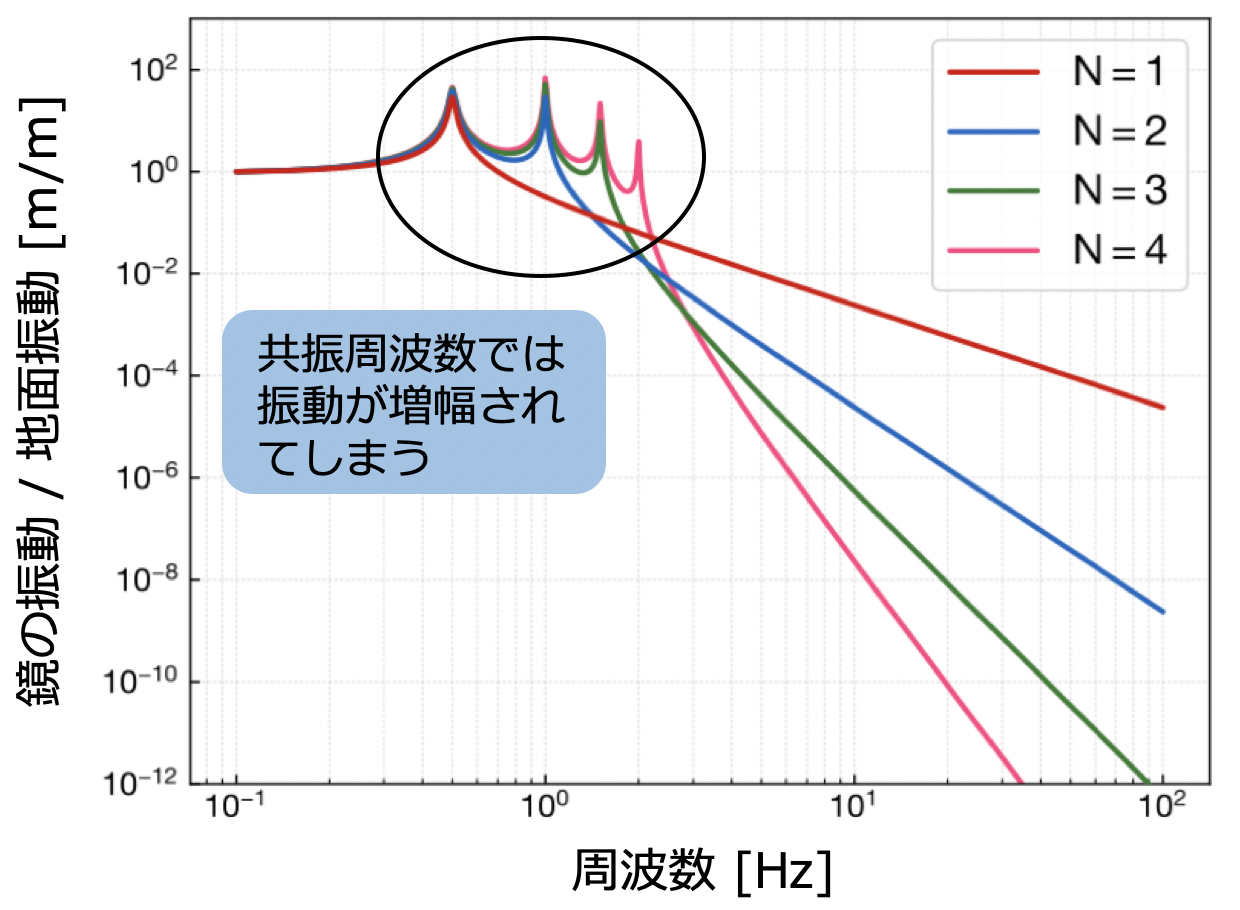
\includegraphics[width=90mm]{fig6_1.png}
\caption[共振周波数における振動の増幅]{多段振り子を用いた防振では共振周波数以上の周波数で高い防振比を得ることができる一方, 共振周波数では鏡に伝わる振動が増幅されてしまう. }
\label{fig6.1}
\end{center}
\end{figure}
第\ref{第3章}章で示した通り, 多段振り子を用いた防振系では共振周波数以上の周波数で高い防振比を得ることができる. その一方で, 共振周波数では鏡に伝わる振動が増幅されてしまう(図\ref{fig6.1}). これでは, 干渉計が安定な状態を保てなくなってしまい, 観測を行うことができない. そこで共振周波数において振動を減衰させるダンピング制御が必要になる. ここで, ダンピング制御とは鏡の変位を局所的にセンサで検出し, それを打ち消す力をアクチュエータによって鏡に加えるフィードバック制御である. つまり, 懸架系にある力(外乱)が加わったとき, 懸架系の応答をフォトセンサが検知し, デジタルシステムに信号を送る. その中でフィルタを通してアクチュエータに信号を送り, 最初に働いた力を打ち消す. そのダイアグラムは図\ref{fig6.2}に示した通りである. 
\begin{figure}[H]
\begin{center}
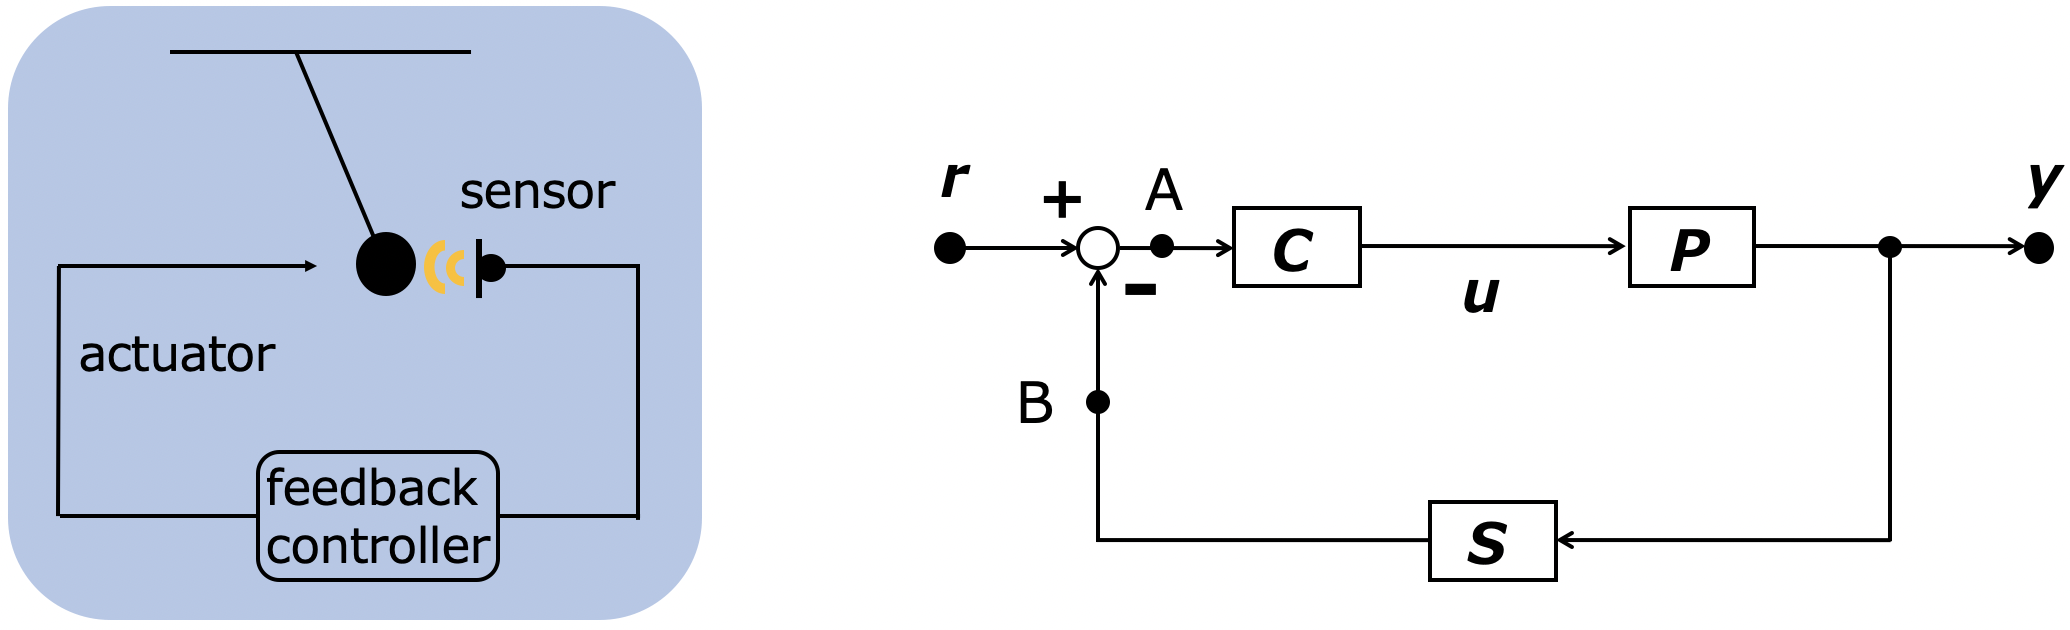
\includegraphics[width=170mm]{fig6_2.png}
\caption[ダンピング制御のダイアグラム]{(左)懸架系のダンピング制御システムの概念図と(右)それと等価なフィードバック制御のブロックダイアグラム. 鏡の変位を局所的にセンサで検出し, それを打ち消す力をアクチュエータによって鏡に加えている. 図中の$C$は制御器, $u$は制御入力, $P$は制御対象, $S$はセンサを表す. また, $r$は目標量, $y$は出力量である.}
\label{fig6.2}
\end{center}
\end{figure}
このときの系の開ループ(open-loop)伝達関数は
\begin{equation}
T_{\rm open}=CP,
\end{equation}
であり, 閉ループ(closed-loop)伝達関数は
\begin{equation}
T_{\rm closed}=\frac{CP}{1+SCP}=\frac{T_{\rm open}}{1+{\rm ST_{\rm open}}},
\end{equation}
と表される. \\
\quad ここで, ダンピングフィルタの実装には一巡伝達関数$ST_{\rm open}$の位相が重要である. ここで, 閉ループではなく開ループ(一巡伝達関数)で考えれば良い理由は以下の通りである. \\
\quad 図\ref{fig6.2}において点Aに単位インパルス\footnote{ディラックのデルタ関数とも呼ばれ, $t\geq0$で連続な任意の関数$f(t)$に対して
\begin{equation}
\int_{-\infty}^{\infty}f(t)\delta(t){\rm d}t=f(0),
\notag
\end{equation}
の作用をする関数である. }を入力したとする. このとき単位インパルスは全ての角周波数成分を含む正弦波のFourier級数に展開できるが, それらの正弦波は点Aから点Bまでの周波数応答特性によって振幅はゲイン倍され, 位相もいくらか遅れて点Bに出力される. \\
\quad このうち位相遅れが$180^{\circ}$である角周波数成分を考える. 位相が$180^{\circ}$ずれているということは正弦波信号の正負が反転するということであるが, 図\ref{fig6.2}において点Bから点Aに戻る際にも正負が反転する. つまり, 点Aに入力された単位インパルスのうち, 位相遅れが$180^{\circ}$である角周波数成分は正負が変わらず点Aに戻ってくる. よってループを一巡したときの振る舞いは扱いの困難な閉ループではなく, 開ループ(一巡伝達関数)を考えれば良い. \\
\quad このとき, $HT_{\rm open}$のゲインが1となる周波数(UGF: Unity Gain Frequency)における位相に気をつける必要がある. \\
\quad 先程と同様に位相遅れが$180^{\circ}$となる角周波数成分を考える. 図\ref{fig6.2}の点Aを出た信号は振幅が開ループのゲイン倍されて戻ってくる. この信号はさらにループを回り, その後も同様に回り続ける. このとき開ループゲインが1より小さければ振幅は減少して閉ループ系は漸近安定になる. 一方で, 開ループゲインが1より大きい場合は振幅が徐々に増大し, 閉ループ系は発散し, 不安定となる. ここで, ナイキスト軌跡(図\ref{fig6.3})が複素数平面上の点(-1+0$j$)を通る場合, 位相遅れが$180^{\circ}$となる角周波数の開ループゲインが1となる. 
\begin{figure}[H]
\begin{center}
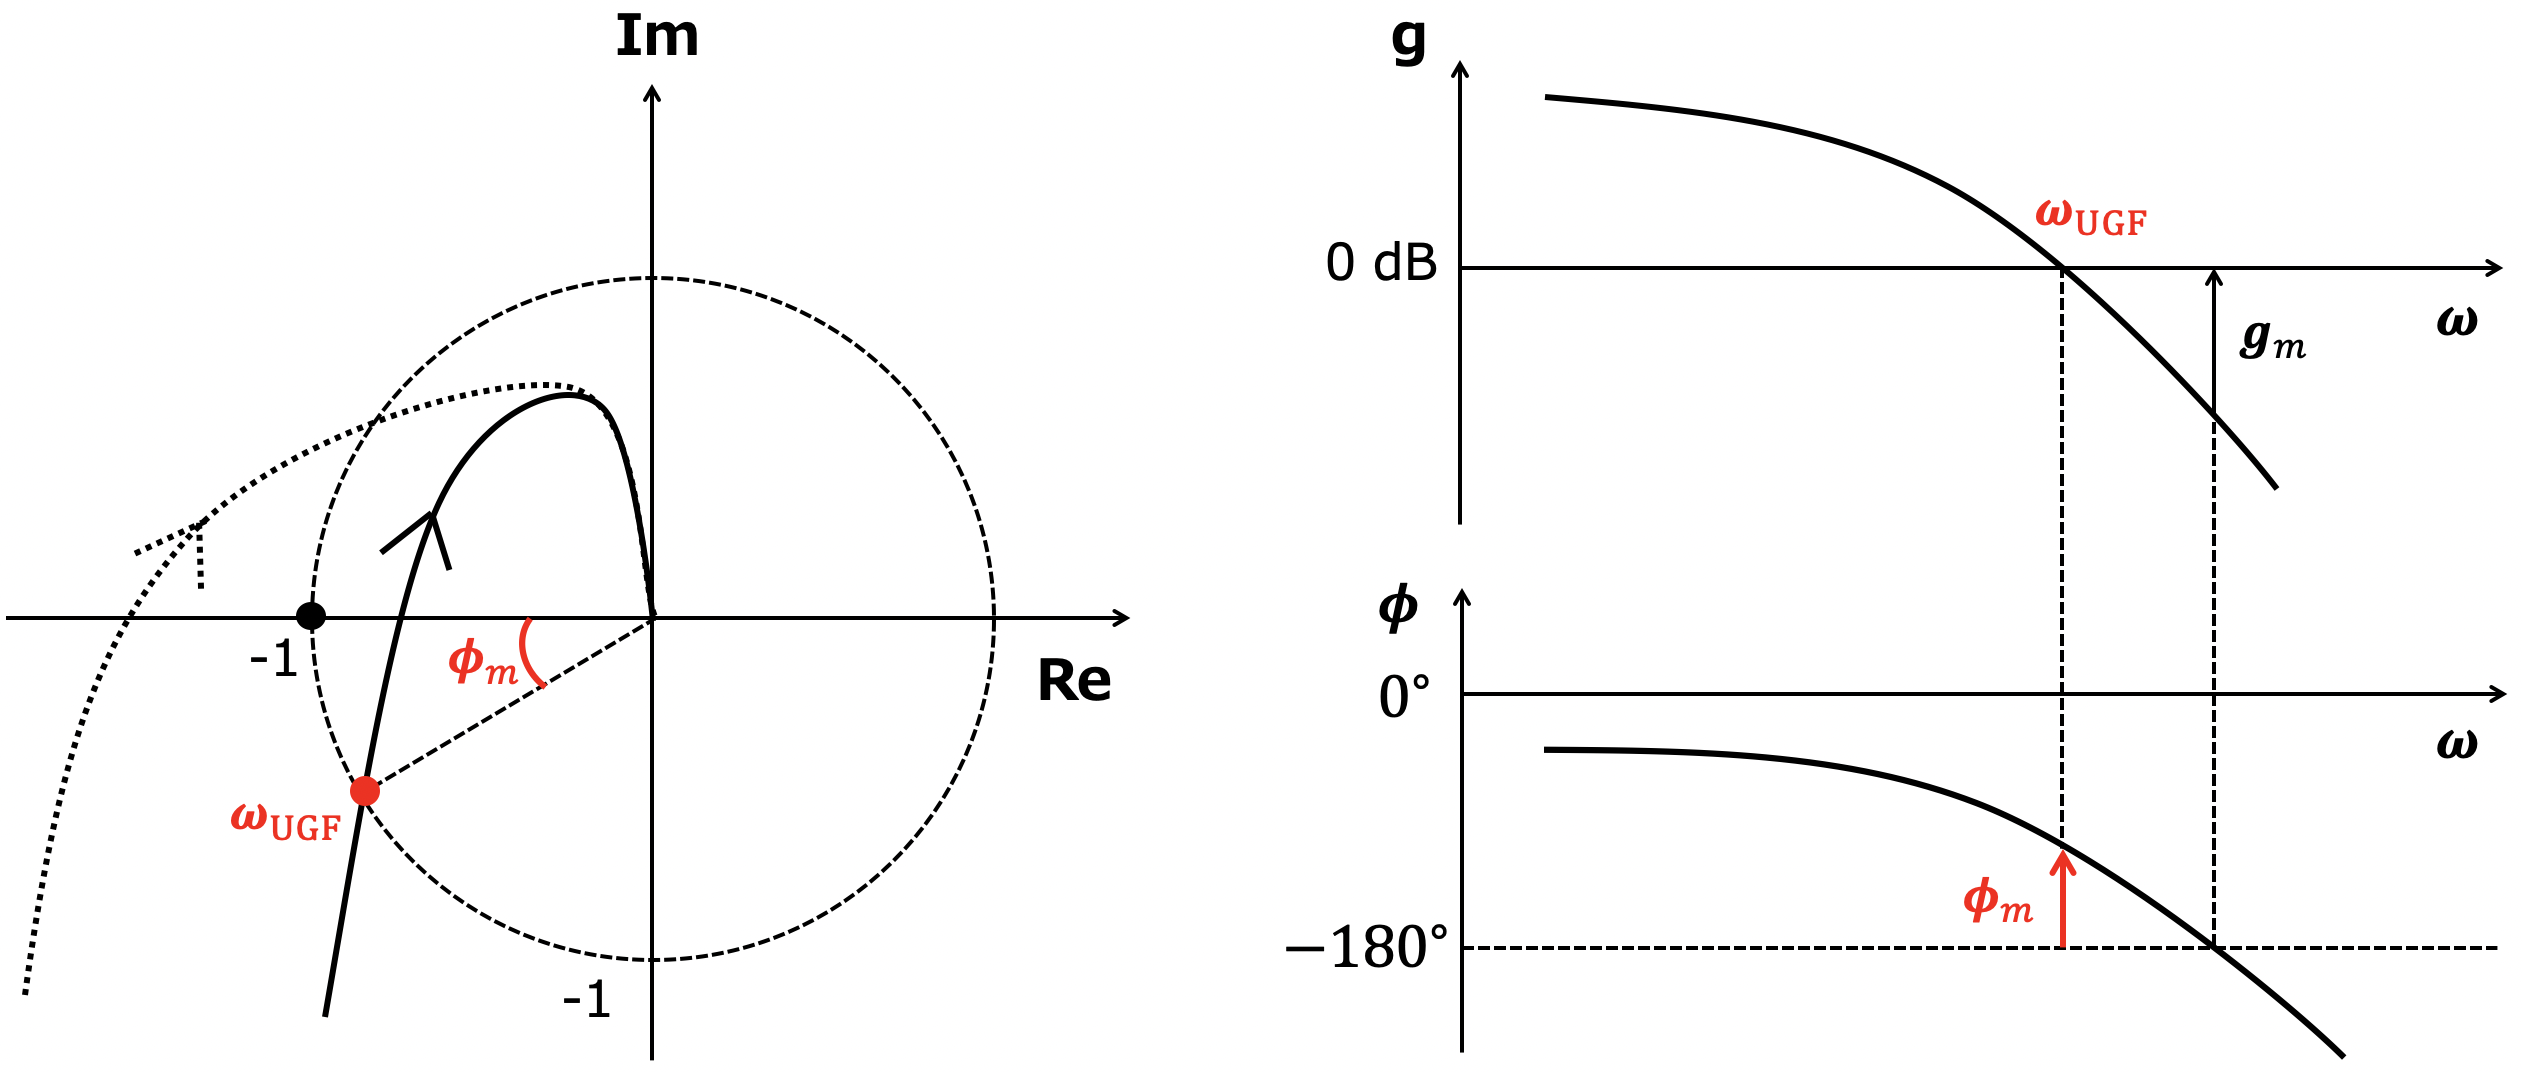
\includegraphics[width=150mm]{fig6_3.png}
\caption[ナイキスト軌跡とボード図]{(左)周波数応答を複素数平面上でベクトルとして表し, その先端を結んで得られる曲線で, ナイキスト軌跡と呼ばれる. UGFはナイキスト軌跡と単位円が交わる点であり, 原点からその点に向かうベクトルの角度を負の実軸から測ったときの角度が位相余裕である. 一巡周波数応答(一巡伝達関数の周波数応答)のベクトル軌跡が(-1+0j)の右側で負の実軸と交われば系は安定, 左側で交われば不安定となる. \\(右)ボード図と呼ばれるもので, 周波数応答と各周波数の関係をゲイン特性曲線, 位相特性曲線で表す. UGFはボード図ではゲイン特性曲線が0 dBの線と交わる点であり, またそのときの位相と-180$^{\circ}$との差が位相余裕である. フィルタを作成する際はボード図を見ながらUGFで位相が180度回っていないか(位相余裕がどの程度あるか)を確認すれば良い. }
\label{fig6.3}
\end{center}
\end{figure}
このときは信号は増大も減少もせず, 点(-1+0$j$)が閉ループ系の安定と不安定の境界となる. つまり, $T_{\rm open}S$のUGFにおいて位相が$180^{\circ}$以上回っていれば, 閉ループ伝達関数$T_{\rm closed}$が発散し, 系のフィードバック制御が成り立たない. \\
\quad すなわち, 安定した系を実現するためには$T_{\rm open}S$のピークにのみゲインを持たせて, このときUGFでの位相が$180^{\circ}$以上回らないようなフィルタを設計する必要がある. ここで, $T_{\rm open}S$に1より大きなゲインを持たせるということは, $T_{\rm closed}$のゲインを下げるということであり, これをダンピングしたい共振周波数に対してのみ行えばよいということである. 
\section{ダンピング制御の原理}
\label{sec6.2}
どのようなフィルタを設計すればよいかをより具体的に考えるために, ダンピング制御の原理について説明する. 先に記述したように懸架系は多段振子であるが, ここでは簡単のため単振子で考える. 速度に比例した項を含めて図\ref{fig6.4}のようなバネで吊るされたモデルを考えと, この系の運動方程式は
\begin{equation}
m\ddot{x}+c\dot{x}+kx=0,
\label{eq6.3}
\end{equation}
となる. ここで$c\dot{x}$は速度に比例した抵抗力である($c$:定数). これを解けば減衰振動に対する解が得られるが, 今は周期的な外力(地面振動など)が加わる強制的な振動を考えるべきであり, この場合式(\ref{eq6.3})は複素数 $z$を用いて
\begin{equation}
\ddot{z}+2\gamma\dot{z}+\omega_0^2z=\omega_0^2a_0{\rm e}^{i\omega t},
\end{equation}
ここで$\gamma=c/2m,\omega_0=\sqrt{k/m}$であり, $a_0:$外力の振幅, $\omega:$外力の角振動数である. 
\begin{figure}[H]
\begin{center}
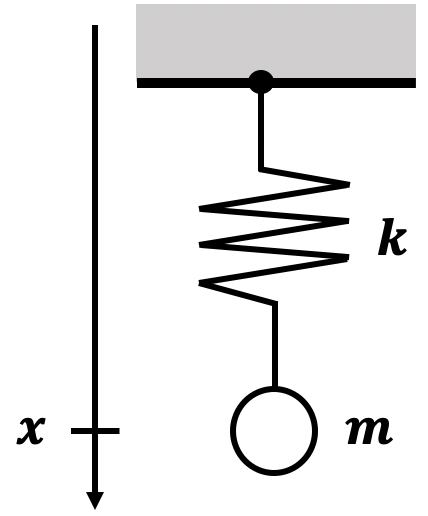
\includegraphics[width=50mm]{fig6_4.png}
\caption[バネ振子によるモデル]{バネ振子によるモデル}
\label{fig6.4}
\end{center}
\end{figure}
この方程式を解くために$z=a{\rm e}^{i\omega t}$とおくと, $\dot{z}=i\omega a{\rm e}^{i\omega t}$, $\ddot{z}=-\omega^2a{\rm e}^{i\omega t}$なので
\begin{equation}
-\omega^2a+2\gamma i\omega a+\omega_0^2a=\omega_0^2a_0.
\end{equation}
これを整理すると
\begin{equation}
a=\frac{\omega_0^2a_0}{\sqrt{(\omega_0^2-\omega^2)^2+4\gamma^2\omega^2}}{\rm e}^{-i\phi}.
\end{equation}
ただし
\begin{equation}
\tan\phi=\frac{2\gamma\omega}{\omega_0^2-\omega^2}.
\end{equation}
これが特解であり, 一般解は外力が0のときの解と合わせたもの\footnote{$\ddot{z}+2\gamma\dot{z}+\omega_0^2z=0$において, 解として$z={\rm e}^{\lambda}t$を仮定して解けばよい. }なので, それは
\begin{equation}
z=a{\rm e}^{-\gamma t}\cos(\omega^{\prime}t+\delta)+\frac{\omega_0^2a_0}{\sqrt{(\omega_0^2-\omega^2)^2+4\gamma^2\omega^2}}\cos(\omega t-\phi).
\label{eq6.8}
\end{equation}
ただし$\omega^{\prime}=\sqrt{\omega_0^2-\gamma^2}$であり, また$a,\delta$は初期条件で決まる値である. \\
\quad 式(\ref{eq6.8})の右辺第1項は十分長い時間で0になるが, 第2項は外力と共に振動を続ける. この振動の振幅
\begin{equation}
|A|=\frac{\omega_0^2a_0}{\sqrt{(\omega_0^2-\omega^2)^2+4\gamma^2\omega^2}},
\end{equation}
を$a_0$で割った値の周波数依存性は図\ref{fig6.5}のようになる. \\
\quad この図より, $\gamma$が非常に小さいときは系が発散し, $\gamma$が小さいとき固有角振動数に近づくと振幅が大きくなるのが分かる(共振). 一方, $\gamma$が大きくなると共振のピークが小さくなっていくが, $\gamma=c/2m$なのでこれは定数$c$を調節することで共振のピークを抑えられる(ダンピングできる)ことを示している. すなわち, ダンピング制御のためには速度に比例した力($c\dot{x}$)を調節するようなフィルタを設計すればよいと分かる. 
\begin{figure}[H]
\begin{center}
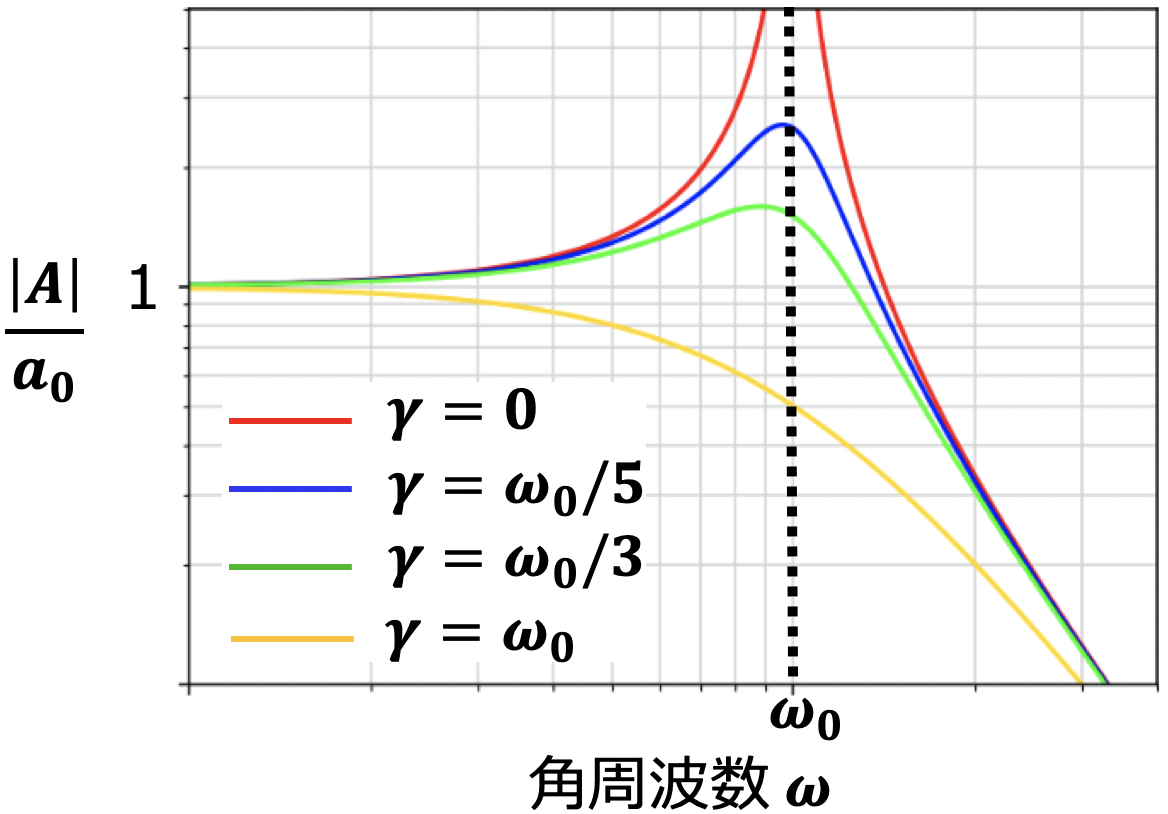
\includegraphics[width=120mm]{fig6_5.png}
\caption[共振の様子を示す曲線]{共振の様子を示す曲線. $\gamma$が大きくなるにつれ, 共振のピークは小さくなっていく. }
\label{fig6.5}
\end{center}
\end{figure}
\begin{figure}[H]
\begin{center}
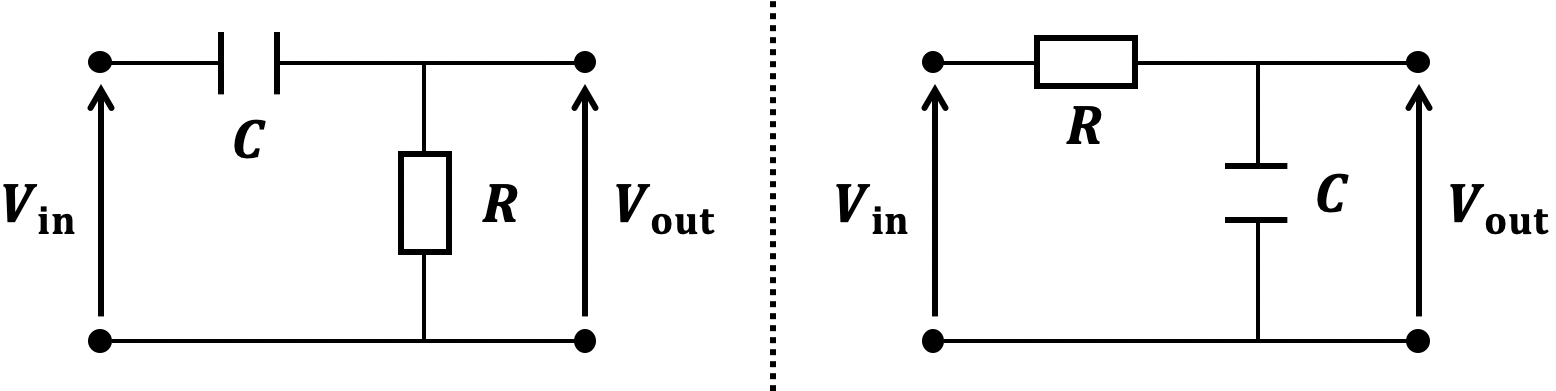
\includegraphics[width=150mm]{fig6_6.png}
\caption[1次のハイパスフィルタ・ローパスフィルタ]{1次のハイパスフィルタ(左)・ローパスフィルタ(右)}
\label{fig6.6}
\end{center}
\end{figure}
ここで, 速度に比例した力を調節するフィルタについて, 典型的な例として1次のハイパスフィルタ・ローパスフィルタを考える. まず1次のハイパスフィルタであるが, コンデンサと抵抗を用いて図\ref{fig6.6}の左側のようになる. 回路に流れる電流を$I$, コンデンサに蓄えられる電荷量をQとすると
\begin{equation}
I=\frac{{\rm d}Q}{{\rm d}t},
\end{equation}
である. 入力信号が入ったとき, コンデンサの両端電圧は$0-V_{\rm in}=-V_{\rm in}$であり, $Q=C\times(-V_{\rm in})$となるので
\begin{equation}
I=\frac{{\rm d}}{{\rm d}t}(-CV_{\rm in})=-C\frac{{\rm d}V_{\rm in}}{{\rm d}t}.
\end{equation}
また, Ohmの法則より$V_{\rm out}=IR$であるから
\begin{equation}
V_{\rm out}=-RC\frac{{\rm d}V_{\rm in}}{{\rm d}t}.
\end{equation}
つまり, ハイパスフィルタを通ると入力信号が微分されて出力される. \\
\quad 例えば入力として大きさ$V_{\rm in}$の矩形波を考えると, 入力の瞬間はコンデンサに電荷が蓄えられないので両端電圧の差は0である. つまり$V_{\rm in}=V_{\rm out}$であり, 抵抗に流れる電流は$I_0=V_{\rm in}/R$となる. この電流によってコンデンサに電荷が蓄えられ, $V_{\rm out}$が徐々に小さくなる. 最終的に矩形波が抜けるとき入力地点の電位が$V_{\rm in}$だけ下がったことになり, これに応じて出力電圧$V_{\rm out}$も$V_{\rm in}$だけ下がる. この後にコンデンサに蓄えられた電荷が放電して入力前の電位に戻る. ここで, 矩形波が時定数$1/RC$に対して十分短ければその形は変わらず出力され, 逆に十分長ければ先に示した通り出力電圧が微分される. つまり, 高周波の信号はそのまま出力するが, 低周波の信号は微分して出力する「ハイパス」フィルタである. \\
\quad 次に1次のローパスフィルタであるが, これもコンデンサと抵抗を用いて図\ref{fig6.6}の右側のように表される. 流れる電流
\begin{equation}
I=\frac{V_{\rm in}}{R},
\end{equation}
によってコンデンサに電荷Qが蓄えられるとすると
\begin{equation}
Q=\int I{\rm d}t,
\end{equation}
であり, このときの出力電圧は
\begin{equation}
V_{\rm out}=-\frac{Q}{C}=-\frac{1}{RC}\int V_{\rm in}{\rm d}t.
\end{equation}
つまり, ローパスフィルタを通ると入力信号が積分されて出力される. \\
\quad 先ほどと同様に大きさ$V_{\rm in}$の矩形波が入力されたとする. その瞬間は出力電圧は0だが, 抵抗$R$を通して電流が流れ徐々に電圧が上がる. その後矩形波が抜ける瞬間はコンデンサの両端の電位差が急に変化するわけではなく, 出力電圧の符号を保ちながら時間と共に放電する. ここで, 矩形波が時定数に対して十分短ければ先に示した通り出力電圧が積分される. 逆に十分長ければその形は変わらず出力される(波形の変化に対してスケールが長い). つまり低周波の信号はそのまま出力するが, 高周波の信号は積分して出力する「ローパス」フィルタである. \\
\quad これらの例をふまえて考えると, 共振ピークのダンピングのためには共振周波数のある領域においてハイパスフィルタがかかるようなフィルタを設計すればよい. すなわちフォトセンサで得た信号を微分してフィードバックすればよいことが分かる. 
\section{ダンピングフィルタの実装とその評価}
\subsection{共振ピークの同定と行列計算}
各懸架装置の各自由度に対し, 共振ピークを同定する必要がある. そのため, まずはアクチュエータで力を加えた際, 懸架系が思い通りの方向に動くかを確認した. これは懸架系の外側にあり, 独立にキャリブレーションされているOpLevの信号を見て行った. その後, アクチュエータで動かした方向とフォトセンサの動作方向の正負が等しいかを確認した後, ホワイトノイズを入れて自由度ごとに励起し, 伝達関数を測定した(図\ref{fig6.7}及び補遺\ref{補遺D}). そこから各自由度の固有モードに対応する共振ピークを特定し, 表\ref{table6.1}$\sim$\ref{table6.4}に示した通りの共振周波数を得た. 
\begin{figure}[H]
\begin{center}
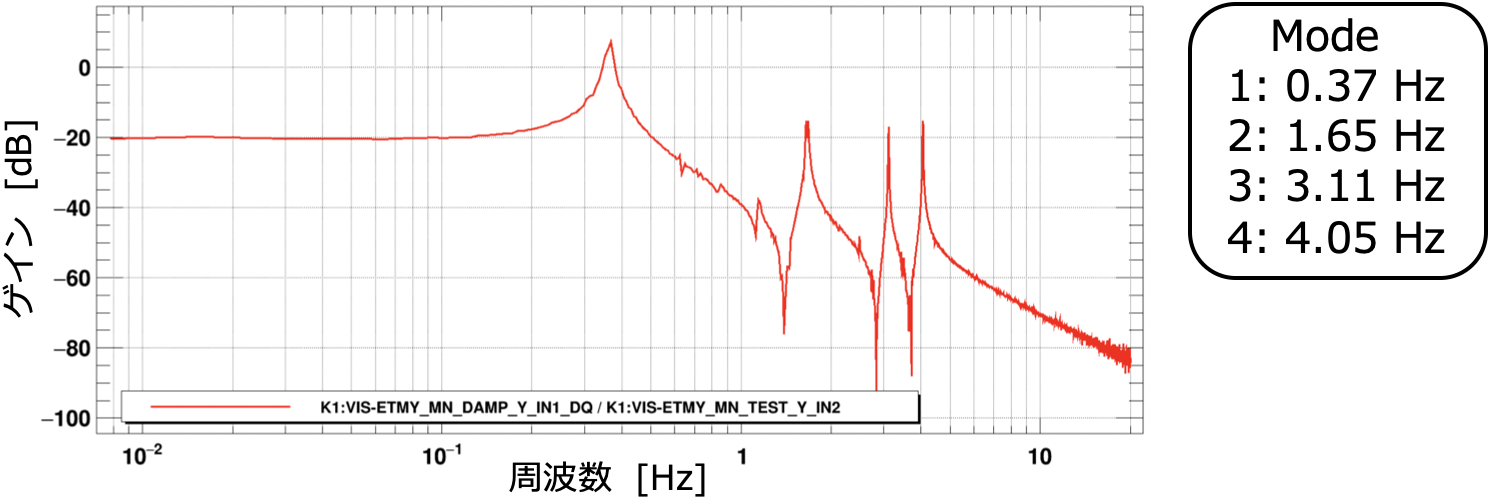
\includegraphics[width=150mm]{fig6_7.png}
\caption[懸架系の応答(ETMY MN Y)]{懸架系の応答(ETMY MN Y). ホワイトノイズを入れてMN段をY方向に励起し, そこからMN段のY方向の動きまでの伝達関数を測定した. 他の懸架系, 自由度の伝達関数については補遺\ref{補遺D}に記した. }
\label{fig6.7}
\end{center}
\end{figure}
\begin{table}[H]
 \centering
  \begin{tabular}{|c||c|c|c|c|}
   \hline
    \diagbox{自由度}{Mode}& 1 & 2 & 3 & 4 \\
   \hline
   L & 0.63 Hz & 1.46 Hz & 2.12 Hz & 2.47 Hz \\
   \hline
   T & 0.63 Hz & 1.49 Hz & 2.12 Hz & 2.49 Hz \\
   \hline
   R & 0.77 Hz & &  &  \\
   \hline
   P & 0.76 Hz & 7.42 Hz &  &   \\
   \hline
   Y & 0.30 Hz & 1.66 Hz & 3.13 Hz & 4.08 Hz \\
   \hline
  \end{tabular}
 \caption[共振周波数 (ETMX)]{共振周波数 (ETMX)}
 \label{table6.1}
\end{table}
\begin{table}[H]
 \centering
  \begin{tabular}{|c||c|c|c|c|}
   \hline
    \diagbox{自由度}{Mode}& 1 & 2 & 3 & 4 \\
   \hline
   L & 0.63 Hz & 1.46 Hz & 2.13 Hz & 2.48 Hz \\
   \hline
   T & 0.63 Hz & 1.52 Hz & 2.09 Hz & 2.516 Hz \\
   \hline
   R & 0.73 Hz & &  &  \\
   \hline
   P & 0.82 Hz & 7.40 Hz &  &   \\
   \hline
   Y & 0.37 Hz & 1.65 Hz & 3.11 Hz & 4.05 Hz \\
   \hline
  \end{tabular}
 \caption[共振周波数 (ETMY)]{共振周波数 (ETMY)}
  \label{table6.2}
\end{table}
\begin{table}[H]
 \centering
  \begin{tabular}{|c||c|c|c|c|}
   \hline
    \diagbox{自由度}{Mode}& 1 & 2 & 3 & 4 \\
   \hline
   L & 0.63 Hz & 1.46 Hz & 2.19 Hz & 2.50 Hz \\
   \hline
   T & 0.63 Hz & 1.45 Hz & 2.13 Hz & 2.49 Hz \\
   \hline
   R & 0.76 Hz & &  &  \\
   \hline
   P & 0.85 Hz & 7.39 Hz &  &   \\
   \hline
   Y & 0.30 Hz & 1.67 Hz & 3.09 Hz & 4.09 Hz \\
   \hline
  \end{tabular}
 \caption[共振周波数 (ITMX)]{共振周波数 (ITMX)}
  \label{table6.3}
\end{table}
\begin{table}[H]
 \centering
  \begin{tabular}{|c||c|c|c|c|}
   \hline
    \diagbox{自由度}{Mode}& 1 & 2 & 3 & 4 \\
   \hline
   L & 0.6328 Hz & 1.461 Hz & 2.188 Hz & 2.500 Hz \\
   \hline
   T & 0.6250 Hz & 1.469 Hz & 2.156 Hz & 2.500 Hz \\
   \hline
   R & 0.7500 Hz & &  &  \\
   \hline
   P & 0.8516 Hz & 7.391 Hz &  &   \\
   \hline
   Y & 0.2969 Hz & 1.672 Hz & 3.094 Hz & 4.086 Hz \\
   \hline
  \end{tabular}
 \caption[共振周波数 (ITMY)]{共振周波数 (ITMY)}
  \label{table6.4}
\end{table}
また, ダンピングフィルタは各自由度に対してかけるので, 自由度ごとに対応するようにフォトセンサの信号を合成している. ここで, フォトセンサが懸架装置の揺れを正確に検知して同程度の出力をすれば, 信号の合成はセンサの幾何学的な配置で決まる. また, アクチュエータについても同様に, 入出力の関係が同じ場合は幾何学的配置に基づいて信号の合成を行えば, それぞれの自由度に対して個別に力を加えることができる. \\
\quad しかし, 自由度にはカップリングが存在し, ある自由度にのみ力を加えるつもりでも, 他の自由度が動いてしまうということがある. よって, 対象の自由度以外に対してダンピング制御を行わないよう, 自由度ごとのカップリングを以下のようにして求める必要がある. \\
\quad まず, 懸架装置を共振周波数で揺らし続ける. この際, その周波数に共振ピークを持たない自由度の揺れは励起されないが, 共振ピークを持つ場合は徐々に揺れが大きくなる. それらの自由度に対し, 揺れの大きさの比を取り, それを打ち消す(decouplingする)ように式(\ref{eq6.16})に示す行列の非対角成分を求める. 
\begin{equation}
\begin{pmatrix}
L^{\prime} \\
T^{\prime} \\
V^{\prime} \\ 
R^{\prime} \\
P^{\prime}\\
Y^{\prime}
\end{pmatrix}=
\begin{pmatrix}
1&C_{TL}&C_{VL}&C_{RL}&C_{PL}&C_{YL}\\
C_{LT}&1&C_{VT}&C_{RT}&C_{PT}&C_{YT}\\
C_{LV}&C_{TV}&1&C_{RV}&C_{PV}&C_{YV}\\
C_{LR}&C_{TR}&C_{VR}&1&C_{PR}&C_{YR}\\
C_{LP}&C_{TP}&C_{VP}&C_{RP}&1&C_{YP} \\
C_{LY}&C_{TY}&C_{VY}&C_{RY}&C_{PY}&1
\end{pmatrix}
\begin{pmatrix}
L\\
T\\
V \\ 
R \\
P \\
Y
\end{pmatrix}.
\label{eq6.16}
\end{equation}
ただし, プライム付き文字が上記の測定で得られた自由度, そうでない文字が真の自由度であり, 非対角成分が自由度ごとのカップリングを表している. 
\subsection{ダンピングフィルタの実装とその効果}
\ref{sec6.2}節で示した通り, 共振周波数が存在する周波数領域において信号を微分して系に返すフィルタを作成すればダンピング制御を実現できる. そこで, フォトセンサで得られた信号に対してそのような動作を行うフィルタをインストールした. 図\ref{fig6.8}はETMXのL方向に対するフィルタを示したものである. \\
\quad 10 Hzあたりまでは共振周波数での振動を抑えるためにハイパスフィルタをかけている. 具体的には25 Hzに極を, 0 Hzに零点を設定しており, この部分が鏡の速度に比例した力を系にフィードバックしている. \\
\quad 一方, ダンピング制御が必要ないそれ以降の周波数領域ではノイズを減らすため\footnote{フィードバック制御におけるノイズについては第\ref{第7章}章参照. }にローパスフィルタをかけている. \\
\quad また, 図\ref{fig6.9}は前小節で記したダンピングフィルタをかけた上で, 励起信号からMNの動きまでの伝達関数を測定した結果を示している. 赤線はフィルタなしの場合であるが, この時は共振周波数において, 揺れが大きくなっているのが分かる. しかし, ダンピングフィルタをかけると青線で示された通り, その揺れが抑えられている. これより, 地震などの何らかの理由により低温懸架装置の共振が励起された場合でも, このフィルタがかけられていれば, その共振をダンプすることができると言える. 
\begin{figure}[H]
\begin{center}
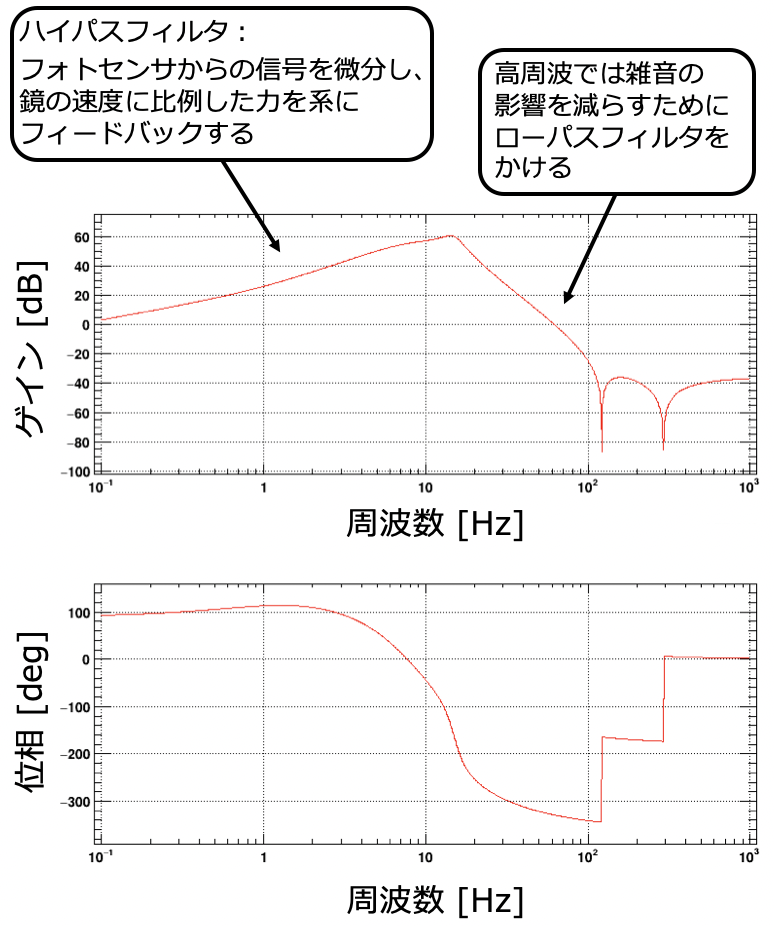
\includegraphics[width=100mm]{fig6_8.png}
\caption[ダンピングフィルタ]{ダンピングフィルタの例(ETMY MN Y). ダンピングしたい共振周波数が存在する低周波では, 鏡の速度に比例した力を系にフィードバックするためのハイパスフィルタをかけている. 一方, 高周波ではノイズの影響を抑えるためにローパスフィルタをかけた. }
\label{fig6.8}
\end{center}
\end{figure}
\begin{figure}[H]
\begin{center}
\includegraphics[width=150mm]{fig6_9.png}
\caption[ダンピングフィルタをかけた時の伝達関数]{ダンピングフィルタをかけた時の伝達関数(ETMY MN段についてY方向に励起し, そこからMN段のY方向の動きまでの伝達関数を測定した). フィルタをかけた場合(青)はフィルタなしの場合(赤)に比べて共振周波数における揺れが抑制されているのが分かる. }
\label{fig6.9}
\end{center}
\end{figure}
\subsection{1/e減衰時間によるダンピング制御の評価}
共振周波数における揺れを抑えられることは分かったが, その抑制にどれだけ時間を要するかという点も, 観測状態への素早い復帰という点で重要である. これは図\ref{fig3.6}に示したCalm-down Phaseにおいて, 各共振モードの振幅が1/eに減衰する時間によって評価される. ここでは5.2.3.1で示したように, 共振周波数に等しい周波数の励起信号を入れた後でその励起を止め, 振動が減衰する時間を測る, という方法で測定を行った. \\
\quad 図\ref{fig6.10}はETMYのYのモード4 (4.08 Hz) の共振について, 励起した揺れが収まるまでの時間をダンピング制御なし, ありの場合で比較したものである. 青線はダンピング制御なしの場合であり, 励起した揺れの振幅が1/eに収まるまでに約97 秒かかっていることが分かった. 一方, ダンピング制御をかけた際の減衰の様子は赤線で示された通りで, 約2 秒で振幅が1/eに収まっているのが分かる. Calm-down Phaseにおける減衰時間に対する要求値は60 秒とされているので, これは十分早く振動を抑えられていると言える. 
\begin{figure}[H]
\begin{center}
\includegraphics[width=150mm]{fig6_10.png}
\caption[励起した共振が収まる様子]{励起した共振が収まる様子. ダンピング制御なし(青)の場合は振動が収まるまでに約97 秒待つ必要があるが, 制御をかけた場合(赤)はそれが2 秒程度に短縮される. }
\label{fig6.10}
\end{center}
\end{figure}
\quad 同様の測定を懸架装置, 自由度に対しても行った(全て常温). 図\ref{fig6.11}$\sim$\ref{fig6.14}および表\ref{table6.5}$\sim$\ref{table6.8}はその結果をまとめたもので, ダンピング制御なしの場合(青点)およびダンピング制御ありの場合(赤点)の, 1/e減衰時間の変化を示している. また, 図中の緑線はCalm-down Phaseにおける減衰時間に対する要求値(60秒)である. \\
\quad これより, 各懸架装置の各自由度の各モードに対して, 要求値を十分満たすダンピング制御を行うことができていると言える. これは外乱などで干渉計のロックが失われた場合でも速やかに再ロックすることが可能であることを意味し, 観測時間の増加につながると期待される. 
\begin{figure}[H]
\begin{center}
\includegraphics[width=175mm]{fig6_11.png}
\caption[1/e減衰時間 (ETMX)]{ダンピングフィルタあり / なしの1/e減衰時間の比較 (ETMX). 青色, 赤色の点がそれぞれダンピングフィルタなし, ありの時の結果を示している. なお, 緑線はLock-acquisition phaseにおける要求値を示しており, ダンピングフィルタを用いると十分早く外乱が抑制されることがこの図から分かる. }
\label{fig6.11}
\end{center}
\end{figure}
\begin{figure}[H]
\begin{center}
\includegraphics[width=175mm]{fig6_12.png}
\caption[1/e減衰時間 (ETMY)]{ダンピングフィルタあり / なしの1/e減衰時間の比較 (ETMY). 青色, 赤色の点がそれぞれダンピングフィルタなし, ありの時の結果を示している. なお, 緑線はLock-acquisition phaseにおける要求値を示しており, ダンピングフィルタを用いると十分早く外乱が抑制されることがこの図から分かる. }
\label{fig6.12}
\end{center}
\end{figure}
\begin{figure}[H]
\begin{center}
\includegraphics[width=175mm]{fig6_13.png}
\caption[1/e減衰時間 (ITMX)]{ダンピングフィルタあり / なしの1/e減衰時間の比較 (ITMX). 青色, 赤色の点がそれぞれダンピングフィルタなし, ありの時の結果を示している. なお, 緑線はLock-acquisition phaseにおける要求値を示しており, ダンピングフィルタを用いると十分早く外乱が抑制されることがこの図から分かる. }
\label{fig6.13}
\end{center}
\end{figure}
\begin{figure}[H]
\begin{center}
\includegraphics[width=175mm]{fig6_14.png}
\caption[1/e減衰時間 (ITMY)]{ダンピングフィルタあり / なしの1/e減衰時間の比較 (ITMY). 青色, 赤色の点がそれぞれダンピングフィルタなし, ありの時の結果を示している. なお, 緑線はLock-acquisition phaseにおける要求値を示しており, ダンピングフィルタを用いると十分早く外乱が抑制されることがこの図から分かる. }
\label{fig6.14}
\end{center}
\end{figure}
\begin{table}[H]
 \centering
  \begin{tabular}{|c||c|c|c|c|c|}
   \hline
    & フィルタ & Mode 1 & Mode 2 & Mode 3 & Mode 4 \\
   \hline
   \multirow{2}{*}{L} & なし &(8.921 $\pm$ 0.174)$\times10^2$ s & (2.702 $\pm$ 0.004)$\times10^2$ s & (4.474 $\pm$ 0.046)$\times10^2$ s & (4.057 $\pm$ 0.007)$\times10^2$ s \\
   \cline{2-6}
      & あり &(1.740 $\pm$ 0.076)$\times10^1$ s & 4.382 $\pm$ 0.706 s & 4.620 $\pm$ 0.296 s & 3.315 $\pm$ 0.555  s \\
   \hline\hline
   \multirow{2}{*}{P} & なし &(1.788 $\pm$ 0.028)$\times10^2$ s & (1.485 $\pm$ 0.001)$\times10^2$ s &  & \\
   \cline{2-6}
      & あり & 5.708 $\pm$ 0.263 s & 8.975 $\pm$ 0.150 s & & \\
   \hline\hline
   \multirow{2}{*}{Y} & なし &(2.509 $\pm$ 0.003)$\times10^2$ s & (4.978 $\pm$ 0.062)$\times10^2$ s & (4.793 $\pm$ 0.023)$\times10^2$ s & (9.708 $\pm$ 0.015)$\times10^1$ s \\
   \cline{2-6}
      & あり & 3.012 $\pm$ 0.227 s & 3.623 $\pm$ 0.086 s & 3.038 $\pm$ 0.105 s & 1.968 $\pm$ 0.212 s \\
   \hline
  \end{tabular}
 \caption[1/e 減衰時間 (ETMX)]{1/e 減衰時間 (ETMX)}
 \label{table6.5}
\end{table}
\begin{table}[H]
 \centering
  \begin{tabular}{|c||c|c|c|c|c|}
   \hline
    & フィルタ & Mode 1 & Mode 2 & Mode 3 & Mode 4 \\
   \hline
   \multirow{2}{*}{L} & なし &(1.381 $\pm$ 0.003)$\times10^3$ s & (4.310 $\pm$ 0.006)$\times10^2$ s & (3.047 $\pm$ 0.028)$\times10^2$ s & (4.790 $\pm$ 0.002)$\times10^2$ s \\
   \cline{2-6}
      & あり &4.691 $\pm$ 0.090 s & (9.685 $\pm$ 0.833)$\times10^{-1}$ s & 1.490 $\pm$ 0.281 s & 2.959 $\pm$ 0.572 s \\
   \hline\hline
   \multirow{2}{*}{P} & なし &(1.313 $\pm$ 0.001)$\times10^2$ s & (1.572 $\pm$ 0.001)$\times10^2$ s & &\\
   \cline{2-6}
     & あり &2.141 $\pm$ 0.027 s & (1.201 $\pm$ 0.007)$\times10^{1}$ s & & \\
   \hline\hline
   \multirow{2}{*}{Y} & なし &(2.691 $\pm$ 0.024)$\times10^2$ s & (6.872 $\pm$ 0.169)$\times10^2$ s & (9.353 $\pm$ 0.025)$\times10^2$ s & (1.167 $\pm$ 0.006)$\times10^2$ s \\
   \cline{2-6}
      & あり &(7.999 $\pm$ 0.024)$\times10^{-1}$ s & 1.921 $\pm$ 0.239 s & 3.057 $\pm$ 0.164 s & 1.560 $\pm$ 0.121 s \\
   \hline
  \end{tabular}
   \caption[1/e 減衰時間 (ETMY)]{1/e 減衰時間 (ETMY)}
    \label{table6.6}
\end{table}
\begin{table}[H]
 \centering
  \begin{tabular}{|c||c|c|c|c|c|}
   \hline
    & フィルタ & Mode 1 & Mode 2 & Mode 3 & Mode 4 \\
   \hline
   \multirow{2}{*}{L} & なし &(1.305 $\pm$ 0.022)$\times10^3$ s & (3.523 $\pm$ 0.014)$\times10^2$ s & (3.585 $\pm$ 0.096)$\times10^2$ s & (4.276 $\pm$ 0.096)$\times10^2$ s \\
   \cline{2-6}
      & あり &8.692 $\pm$ 0.695 s & 2.429 $\pm$ 0.714 s & 5.088 $\pm$ 0.135 s & 2.020 $\pm$ 0.454 s \\
   \hline\hline
   \multirow{2}{*}{P} & なし &(1.710 $\pm$ 0.109)$\times10^2$ s & (1.493 $\pm$ 0.001)$\times10^2$ s & &  \\
   \cline{2-6}
     & あり & 2.475 $\pm$ 0.123 s & (1.369$\pm$0.004)$\times10^1$ s & &  \\
   \hline\hline
   \multirow{2}{*}{Y} & なし &(3.026 $\pm$ 0.037)$\times10^2$ s & (7.105 $\pm$ 0.043)$\times10^2$ s & (7.260 $\pm$ 0.202)$\times10^2$ s & (1.067 $\pm$ 0.006)$\times10^2$ s \\
   \cline{2-6}
      & あり &2.228 $\pm$ 0.075 s & 2.788 $\pm$ 0.161 s & 4.659 $\pm$ 0.085 s & 2.118 $\pm$ 0.084 s \\
   \hline
  \end{tabular}
  \caption[1/e 減衰時間 (ITMX)]{1/e 減衰時間 (ITMX)}
   \label{table6.7}
\end{table}
\begin{table}[H]
 \centering
    \begin{tabular}{|c||c|c|c|c|c|}
   \hline
    & フィルタ & Mode 1 & Mode 2 & Mode 3 & Mode 4 \\
   \hline
   \multirow{2}{*}{L} & なし &(5.475 $\pm$ 0.065)$\times10^2$ s & (2.126 $\pm$ 0.004)$\times10^2$ s & (2.435 $\pm$ 0.027)$\times10^2$ s & (2.446 $\pm$ 0.070)$\times10^2$ s \\
   \cline{2-6}
      & あり &3.890 $\pm$ 0.110 s & 1.169 $\pm$ 0.150 s & 6.251 $\pm$ 0.152 s & 1.318 $\pm$ 0.256 s \\
   \hline\hline
   \multirow{2}{*}{P} & なし &(1.455 $\pm$ 0.035)$\times10^2$ s & (1.457 $\pm$ 0.001)$\times10^2$ s & &   \\
   \cline{2-6}
     & あり &1.724 $\pm$ 0.114 s & (1.093 $\pm$ 0.006)$\times10^{1}$ s & &  \\
   \hline\hline
   \multirow{2}{*}{Y} & なし &(4.674 $\pm$ 0.005)$\times10^2$ s & (4.553 $\pm$ 0.117)$\times10^2$ s & (1.587 $\pm$ 0.008)$\times10^3$ s & (8.667 $\pm$ 0.001)$\times10^2$ s \\
   \cline{2-6}
      & あり &1.441 $\pm$ 0.011 s & 1.942 $\pm$ 0.074 s & 3.994 $\pm$ 0.177 s & 1.859 $\pm$ 0.071 s \\
   \hline
  \end{tabular}
  \caption[1/e 減衰時間 (ITMY)]{1/e 減衰時間 (ITMY)}
   \label{table6.8}
\end{table}
\section{冷却した際の制御の変更}
第\ref{第5章}章において測定した82 KにおけるETMXの伝達関数, 共振周波数を測定した. 伝達関数の形に大きな変化は見られず, また共振周波数は数パーセント高くなっただけであり, それによるUGFでの位相余裕の変化は少なかった. そこで, 297 Kでのダンピング制御のゲインだけを変えて82 Kにおける1/e 減衰時間を測定したところ図\ref{fig6.15}および表\ref{table6.9}のようになった. 
\begin{figure}[H]
\begin{center}
\includegraphics[width=175mm]{fig6_15.png}
\caption[82 Kにおける1/e減衰時間 (ETMX)]{82 Kにおけるダンピングフィルタあり / なしの1/e減衰時間の比較 (ETMX). 青色, 赤色の点がそれぞれダンピングフィルタなし, ありの時の結果を示している. 297 Kの場合の制御からゲインを変更しただけであるが, 要求に対して十分早く振動を抑えることができており, 冷却によってダンピング制御に大幅な変更を加える必要がないことが分かる. }
\label{fig6.15}
\end{center}
\end{figure}
\begin{table}[H]
 \centering
  \begin{tabular}{|c||c|c|c|c|c|}
   \hline
    & フィルタ & Mode 1 & Mode 2 & Mode 3 & Mode 4 \\
   \hline
   \multirow{2}{*}{L} & なし &(7.569 $\pm$ 0.070)$\times10^2$ s & (2.629 $\pm$ 0.008)$\times10^2$ s & (6.312 $\pm$ 0.009)$\times10^2$ s & (2.555 $\pm$ 0.004)$\times10^2$ s \\
   \cline{2-6}
      & あり &(1.014$\pm$0.097)$\times10^1$ s & 3.366 $\pm$ 0.932 s & 9.279 $\pm$ 0.433 s & 2.683 $\pm$ 0.578 s \\
   \hline\hline
   \multirow{2}{*}{P} & なし &(1.745 $\pm$ 0.004)$\times10^2$ s & (1.839 $\pm$ 0.002)$\times10^2$ s & &  \\
   \cline{2-6}
     & あり & 4.342 $\pm$ 0.017 s & 8.057 $\pm$ 0.129 s & &  \\
   \hline\hline
   \multirow{2}{*}{Y} & なし &(1.377 $\pm$ 0.007)$\times10^2$ s & (3.414 $\pm$ 0.003)$\times10^2$ s & (5.373 $\pm$ 0.002)$\times10^2$ s & (1.754 $\pm$ 0.001)$\times10^2$ s \\
   \cline{2-6}
      & あり &2.377 $\pm$ 0.245 s & 3.980 $\pm$ 0.232 s & 6.555 $\pm$ 0.156 s & 3.327 $\pm$ 0.063 s \\
   \hline
  \end{tabular}
  \caption[1/e 減衰時間 (ETMX 82 K)]{1/e 減衰時間 (ETMX 82 K)}
   \label{table6.9}
\end{table}
これより, 297 Kにおけるダンピング制御のゲインを変えるだけで, 82 Kでも60 秒以内に振動がおさまるという要求を十分満たすことができると言える. つまり, 冷却に伴う懸架装置の特性の変化により, 制御の大幅な変更の必要性は生じず, ゲインを調整するだけで良いことが分かった.

\chapter{制御雑音の低減}
\label{第7章}
\fontsize{11pt}{16pt}\selectfont
\section{制御雑音}
\begin{figure}[H]
\begin{center}
\includegraphics[width=120mm]{fig7_1.png}
\caption[制御雑音]{制御系には外乱と雑音が存在する. 図中の$d$は外乱, $n$は雑音, $r$は目標値, $y$は制御量を表す. }
\label{fig7.1}
\end{center}
\end{figure}
図\ref{fig7.1}において, 一巡伝達関数を$T_{\rm loop}=T_{\rm open}S=CPS$と書くと, 外乱$d$から制御量$y$, 雑音$n$から制御量$y$までの伝達関数はそれぞれ
\begin{equation}
T_{dy}\equiv\frac{y}{d}=\frac{P}{1+T_{\rm loop}}, 
\label{eq7.1}
\end{equation}
\begin{equation}
T_{ny}\equiv\frac{y}{n}=\frac{T_{\rm loop}}{1+T_{\rm loop}}, 
\label{eq7.2}
\end{equation}
となる. また, 目標値$r$から制御量$y$の伝達関数を制御系の特性とすると, その値は
\begin{equation}
T_{ry}\equiv\frac{y}{r}=\frac{CP}{1+CPS}=\frac{CP}{1+T_{\rm loop}}, 
\end{equation}
である. ここで, 制御対象が$P\rightarrow P+\Delta P$となったとき, 制御系の特性の変動は
\begin{equation}
\Delta T_{ry}=\frac{\Delta P}{1+C(P+\Delta P)S}\times\frac{T_{ry}}{P}, 
\label{eq7.4}
\end{equation}
となる. このとき微分感度は
\begin{equation}
S_0=\lim_{\Delta P\rightarrow 0}\frac{\Delta T_{ry} / T_{ry}}{\Delta P / P}, 
\label{eq7.5}
\end{equation}
と定義される. ただし, $\frac{\Delta T_{ry} / T_{ry}}{\Delta P / P}$は相対感度と呼ばれ, この値が1より小さい時は外乱に対して制御特性が変動しにくいことを意味している. \\
\quad 式(\ref{eq7.4}), (\ref{eq7.5})より, 
\begin{equation}
S_0=\lim_{\Delta P\rightarrow 0}\frac{\left(\frac{\Delta P}{1+C(P+\Delta P)S}\times\frac{T_{ry}}{P}\right) / T_{ry}}{\Delta P / P}=\frac{1}{1+CPS}=\frac{1}{1+T_{\rm loop}}, 
\label{eq7.6}
\end{equation}
と書くことができるので, 式(\ref{eq7.1})より
\begin{equation}
T_{dy}=S_0P, 
\label{eq7.7}
\end{equation}
である. また, 式(\ref{eq7.2})から
\begin{equation}
S_0+T_{ny}=1, 
\label{eq7.8}
\end{equation}
と書ける. このとき, 外乱の影響を小さくする, すなわち$T_{dy}$を小さくしようとすると式(\ref{eq7.7})より, $S_0$も小さくなる. すると式(\ref{eq7.8})より, $T_{ny}$が大きくなる. \\
\quad つまり, ダンピングフィルタをかけて振動を抑えようとする(=外乱を抑えようとする)と雑音の影響が大きくなってしまう. また, 逆に雑音を減らそうとすると外乱の影響が大きくなる. 例えば$S$にローパス特性を持たせる(=高周波帯において$T_{\rm loop}$を小さくする)などしても, 式(\ref{eq7.6})より$S_0$が大きくなるため, 式(\ref{eq7.7})より$T_{dy}$も大きくなるのである. \\
\quad このように, ダンピング制御と雑音はトレードオフの関係にある. よって, 低周波帯では振動減衰を, 高周波帯では雑音低減を重視するというような制御がよく用いられる. \\
\quad しかし, 図\ref{fig3.7}に示したLock-acquisition PhaseではFP共振器を素早くロックすることが目標であるため, 広い帯域で強い制御をかける必要がある. 一方, Observation Phaseにおいては安定な干渉計ロックを保持できるレベルの制御で十分であり、それよりも雑音の低減を目指すべきである. 前回の観測 (O3GK) では懸架系の制御がLock-acquisition Phase のままであったが, 本研究では, Observation Phaseにおける低雑音な制御を行うことを目標とした. 以下の節でそれを述べる. 
\section{制御フィルタの変更}
まず, Type-A suspensionのうち, ETMY, ITMX, ITMYの3つに対してObservation Phaseにおける制御フィルタ(以下Observation フィルタ)を作成した. ここではITMXについて実際のフィルタを示しながらその設計について記載する.
%まず, Observation Phaseにおける制御フィルタ(以下Observation フィルタ)を作成した. ただし, ETMXはテストマスに干渉計の信号がフィードバックされており, 干渉計の長さを決めている.そのため, FPMIの時点で制御を変えてしまうと, PRFPMIを構成した際に問題が生じる. よって本論文ではType-A suspensionのうち, ETMY, ITMX, ITMYの3つを低雑音制御の対象とする. 
\subsection{ITMX Length}
まずL方向について, フォトセンサの出力信号からダンプしすぎている周波数がないか確かめた(図\ref{fig7.2}). そして, そのスペクトルからどのくらいオーバーダンプしているかを見積もり, その分だけダンピングフィルタのゲインを下げた. さらに共振の位置にノッチフィルタを入れてピークを潰し, 10 Hz以上では4次の楕円ローパスフィルタによって, 従来以上に急峻にゲインを落とした(楕円フィルタは同じ次数を持った他のフィルタに比べて, ゲインの変化が最も早いという特性を持つフィルタである). その後1晩放置し, 信号が発振しないことを確かめた. 最終的なフィルタは図\ref{fig7.3}の通りである.
\begin{figure}[H]
\begin{center}
\includegraphics[width=140mm]{fig7_2.png}
\caption[フォトセンサのエラー信号 (ITMX MN L)]{フォトセンサのエラー信号 (ITMX MN L). 落ち込んでいる部分が共振ピークでの揺れをダンピングしている箇所であり, エラー信号のレベルに対してどの程度小さくなっているかという値からオーバーダンプの度合いを見積もっている.}
\label{fig7.2}
\end{center}
\end{figure}
\begin{figure}[H]
\begin{center}
\includegraphics[width=160mm]{fig7_3.png}
\caption[Observation フィルタ (ITMX L)]{赤線がObservation フィルタ (ITMX L), 青線がLock-acquisition phaseで用いられるフィルタをかけた時のMNの応答を表す. Lock-acquisition phaseで用いるフィルタよりもゲインを下げ, 共振ピークをノッチで潰した上, 10 Hz以上では楕円フィルタによって急峻にゲインを下げている.}
\label{fig7.3}
\end{center}
\end{figure}
\subsection{ITMX Pitch}
P, Y方向のフォトセンサのダンピング制御はObservation phaseでは完全にオフにし, OpLevを用いて制御を行う. これはP, Y方向に関しては, OpLevを用いた方が制御雑音が小さいことが分かっているからである. \\
\quad Lの場合と同様にしてゲインの下げ方を調べた. その結果0.2 Hz前後をUGFとしてゲインを下げればよいことが分かった. そこで, UGFでの位相の回りに注意しながら0.4 Hzから4次楕円ローパスフィルタをかけた. さらに共振の位置にノッチフィルタを入れてピークを潰し, しばらく放置して安定であることを確かめた.\\
\quad 実際に設計したフィルタを図\ref{fig7.4}に示す. 赤線がObservation フィルタを表しており, UGFは0.191 Hz, そこでの位相余裕は$21^{\circ}$となっている.
\begin{figure}[H]
\begin{center}
\includegraphics[width=170mm]{fig7_4.png}
\caption[Observation フィルタ (ITMX P)]{赤線がObservation フィルタ (ITMX P), 青線がLock-acquisition phaseで用いられるフィルタをかけたときのMNの応答を表す. なお, Observation フィルタについて, UGFは0.191 Hzであり, そこでの位相余裕は$21^{\circ}$である.}
\label{fig7.4}
\end{center}
\end{figure}
同様の制御をITMY, ETMYにも実装し, 制御雑音を測定した.
\section{制御雑音の測定}
\subsection{測定方法}
まずFPMI(第\ref{第2章}章参照)をロックする. このFPMIにおいて, 重力波信号は腕の差動信号であり, DARM信号と呼ばれている. また, DARM信号は図\ref{fig7.5}においてPDに向かって来るので, そこで取得される. その信号を用いてETMXにフィードバック信号を返し, 腕の差動変異を保つようにETMXを駆動している.
\begin{figure}[H]
\begin{center}
\includegraphics[width=120mm]{fig7_5.png}
\caption[FPMIの構成とDARM信号]{FPMIの構成とDARM信号}
\label{fig7.5}
\end{center}
\end{figure}
次に, 制御雑音を測定するために, 各懸架装置を各自由度に振動させ, その動きからDARM信号までの伝達関数を測定した. 測定した伝達関数の例を図\ref{fig7.6}に示す. 
\begin{figure}[H]
\begin{center}
\includegraphics[width=120mm]{fig7_6.png}
\caption[ITMX MN Pの出力からDARM信号までの伝達関数]{ITMX MN Pの出力からDARM信号までの伝達関数}
\label{fig7.6}
\end{center}
\end{figure}
懸架装置をこのように振動させていない時でも, 制御に用いるセンサの雑音は常に存在している. そこで各自由度の出力の振幅スペクトル密度 (Amplitude Spectrum Density: ASD)  $S_{\rm SUMOUT}$を測定した伝達関数${\rm TF}_{\rm SUMOUT}$にかけることによって, 制御雑音が得られる. 
\begin{equation}
N_{\rm control}={\rm TF}_{\rm SUMOUT}\times S_{\rm SUMOUT}.
\end{equation}
さらに、各懸架装置の制御雑音は無相関であるから, ETMXを除くType-A suspensionの制御雑音の2乗和を取ることで, 全体の制御雑音が得られる. 
\begin{equation}
N_{\rm control, all}=\sqrt{N_{\rm control, ETMY}^2+N_{\rm control, ITMX}^2+N_{\rm control, ITMY}^2}.
\label{eq7.10}
\end{equation}
\subsection{測定結果}
作成したObservation フィルタを使用した場合と, しなかった場合について, 式(\ref{eq7.10})の計算をした結果を図\ref{fig7.7}に示した. 
\begin{figure}[H]
\begin{center}
\includegraphics[width=160mm]{fig7_7.png}
\caption[Observation フィルタの効果]{Observation フィルタの効果. Observation フィルタを用いることにより, 低温懸架装置の制御雑音が$2\sim3$ 桁小さくなっており, これはO4a観測における目標感度 (3 Mpc) と比べても小さい. }
\label{fig7.7}
\end{center}
\end{figure}
図中の緑線がObservationフィルタなしの場合, オレンジの線がObservationフィルタありの場合を示している. これより, Observationフィルタを使用することで, ETMXを除く低温懸架装置の制御雑音が$2\sim3$ 桁小さくなっているのが分かる. また, Observationフィルタを使用した場合の制御雑音は, O4a観測(Observation 4の初めの段階)における目標感度 (3 Mpc) と比べても小さいと分かる.\\
\quad さらに, 図\ref{fig7.8}に現在のFPMIの感度(赤)とObservationフィルタありの場合の制御雑音(オレンジ), および各懸架装置の各自由度についての制御雑音を示した. これより, 幅広い帯域でETMYのYに対する制御雑音が支配的であることが分かる. また, この図に示された懸架装置の違いによる制御雑音の差を埋めることは, 今後の課題である.
\begin{figure}[H]
\begin{center}
\includegraphics[width=160mm]{fig7_8.png}
\caption[懸架装置, 自由度ごとの制御雑音]{懸架装置, 自由度ごとの制御雑音. ETMYのYに対する制御が最も大きな雑音を生んでいる.}
\label{fig7.8}
\end{center}
\end{figure}
なお, 現在$10\sim50$ Hzにおいて, まだObservationフィルタを実装していないETMXの制御雑音が他の低温懸架装置と比べて著しく大きいでことは判明している(図\ref{fig7.9}). しかし, 本研究の成果より, ETMXに対しても同様の制御を実装すれば, O4観測にとって十分なレベルまで制御雑音を低減可能であると推察される.
\begin{figure}[H]
\begin{center}
\includegraphics[width=160mm]{fig7_9.png}
\caption[ETMXの制御雑音]{ETMXの制御雑音. 現在はETMXの制御雑音が著しく大きい. しかし, 他の低温懸架装置と同様の制御を実装すれば, O4観測に十分なレベルまで制御雑音を低減できると考えられる.}
\label{fig7.9}
\end{center}
\end{figure}
また, 新たに設計した制御を用いてもFPMIが安定に動作するかどうかを確かめた. 図\ref{fig7.10}はその時の干渉計の状態を示している. 図中のFPMI Lockedは従来の制御フィルタを用いてFPMIをロックしている状態であり, Observationが低雑音制御に切り替えた状態である. 2023年1月4日の13時43分にFPMI LockedからObservationに切り替え, 2023年1月5日の13時46分までの約26 時間, FPMIが安定に動作することが確かめられた. なお, 2023年1月5日の13時46分にFPMIのロックを落としたのは, 干渉計作業のためであり, これは人為的なものである.
\begin{figure}[H]
\begin{center}
\includegraphics[width=160mm]{fig7_10.png}
\caption[FPMIの安定性]{Observatiobフィルタを用いた際のFPMIの安定性. FPMI Locked, Observationはそれぞれ従来の制御, 新しく設計した制御を用いてFPMIをロックしている状態である. 2023年1月4日の13時43分にFPMI LockedからObservationに切り替え, 人為的にロックを落とした2023年1月5日の13時46分までの約26 時間, FPMIが安定に動作することを確かめた.}
\label{fig7.10}
\end{center}
\end{figure}

\section{制御雑音低減のまとめ}
ETMY, ITMX, ITMYの低温懸架装置に対して制御雑音の低減を目指したObservation フィルタを作成し, $10\sim100$ Hzにおいて制御雑音を$2\sim3$ 桁低減することに成功した.  未実装のETMXに対しても同様の制御を行うことにより, O4観測における制御雑音低減の目標を完全に達成することが期待される. また, 新たに設計した制御を用いてもFPMIを長時間安定に動作できることを確認した. \\
\quad しかし, O5観測では128 Mpcが目標感度とされており, それを実現するためには低温懸架装置の制御雑音をさらに低減する必要がある. それを実現するためには様々なアプローチが考えられ, 例えば振動をモードごとに分解してそれらを独立に減衰させる手法などが考えられる. これにより, ダンピング性能と制御雑音の最適化が容易となり, 効率良く制御を行えるようになると期待できる\cite{modal}. あるいは, 現在ダンピング制御に用いられているフォトセンサよりも高性能なセンサの開発や, PやY方向のカップリングに関係するビームのアラインメント技術を向上させるなども有効であると考えられる. これについては今後の研究で検討, 実装していく必要がある.










\chapter{結論}
\label{第8章}
\fontsize{11pt}{16pt}\selectfont
\section{結論}
本研究ではKAGRAのサファイア鏡を吊るした低温懸架装置の一つであるETMXについて, 82 Kにおける特性を評価した. その結果, 先行研究で行われた測定と同様, 低温にするとフォトセンサの出力が1.8倍大きくなることが分かった. 一方で, MN段とIM段で用いられる12個のセンサの出力の範囲は, 82 Kにおいて平均値に対して32\%のばらつきがあることが新たに分かった. この結果はばらつきの範囲が50\%以下におさまる必要があるというKAGRAでの要求値を満たす. しかし, 冷却することによって出力にばらつきの範囲が徐々に大きくなるという結果も得られているため, 今後冷却が進んでも要求を満たすかどうかは, 注意して確認する必要がある. また, ETMXの機械的な共振周波数およびその伝達関数の低温にした際の変化量を測定した. その結果, 冷却に伴う特性の変化は軽微で、制御系に大きな変更を加える必要がないことを確かめた.\\
\quad また, 低温懸架装置の共振周波数では, サファイア鏡に伝わる地面の振動が増幅されてしまうので, その振動を抑える必要がある. そこで, 懸架装置の変位をフォトセンサで検知し, 速度に比例した力をアクチュエータを通じて鏡にフィードバックするというダンピング制御を全ての低温懸架装置に対して行った. そして, そのダンピング制御が共振周波数における振動を60 秒以内に減衰させるという要求を満たすものであることを確認した. これにより, 外乱などで干渉計のロックが失われた場合でも速やかに再ロックすることが可能となり, 観測時間の増加につなげることができる.\\
\quad さらに, 2020年3月のO3GKでは低温懸架装置の制御雑音が$10\sim50$ Hzにおける感度を制限していたことを踏まえ, ETMX以外の低温懸架装置に対して観測時に用いる低雑音な制御フィルタを新たに設計した. その結果, $10\sim50$ Hzにおいて, 新たに設計した制御フィルタの制御雑音が既存のフィルタの制御雑音と比べて$2\sim3$桁低減することを確認した. また, その制御を用いてもFPMIが安定に動作することを確かめた.
\section{今後の展望}
2023年3月からのO4観測に向けて, ETMXはさらに冷却される. 冷却が進んだ際は特性評価を全ての低温懸架装置に対して行い, 冷却したことによるフォトセンサのばらつきの程度や制御の変更の必要性を検討し, 必要なら改良を行う. また, 冷却が進んでおらず, 低温化に伴う特性評価の対象としなかったETMX以外の低温懸架装置も今後冷却されるため, 同様の特性評価を行う予定である. 制御雑音については, 本研究で設計した新しい制御が未実装のETMXに対しても同様の制御を行うことにより, $10\sim50$ HzにおけるKAGRAの感度の向上に貢献する. \\
\quad また, O5観測では128 Mpcを目標感度としており, さらなる感度の向上が必要となる(図\ref{fig8.1}). そこで, 低温懸架装置の振動をモードごとに分解してそれらを独立に減衰させることを考える。これにより, 精密な数値シミュレーションに基づいて, ダンピング性能と制御雑音の最適化が容易になり, 効率良くダンピングを行えるほか, 懸架装置ごとの制御雑音の違いについてもより詳細に分析してその雑音の低減を達成できると考えられる. 他にも高性能な低温センサを開発するなど, さまざまな観点から制御雑音の低減を図る. これによって, 低周波における感度を向上してインスパイラルフェイズの重力波を詳細に観測し, 中性子星の質量をより正確に得ることを目指す. こうして得られた中性子星の質量は, 合体フェイズ以降の重力波から得られる中性子星の構造情報と合わせることで, 中性子星物質の状態方程式に制限をつけることができる. これは天文学や宇宙物理学, さらには原子核物理や素粒子物理など幅広い分野の発展につながることが期待される.
\begin{figure}[H]
\begin{center}
\includegraphics[width=140mm]{fig8_1.png}
\caption[O5観測での目標感度と現在の制御雑音]{O5観測での目標感度と現在の制御雑音. ピンクの線はO5での目標感度である128 Mpcを示している. この感度を達成するためには, $10\sim50$ Hzにおいて制御雑音を$1\sim3$ 桁程度低減する必要がある. そこで, 精密な数値シミュレーションに基づくモーダルダンピングなど, 様々な観点で制御雑音の低減, 感度の向上を目指す.}
\label{fig8.1}
\end{center}
\end{figure}



\appendix
\def\thechapter{\Alph{chapter}}
\def\chaptername{補遺}
\def\chapternamew{}
\renewcommand{\appendixname}{補遺}
\chapter{反バネ効果による低周波防振}
\label{補遺A}
\fontsize{11pt}{16pt}\selectfont
重力波観測帯域における防振には第\ref{第3章}章で述べたように多段振り子を用いる方法と, 振り子の共振周波数をより低周波にする方法がある. この内, 後者を実現するためにKAGRAでは Inverted Pendulum (IP: 倒立振子)と Geometric Anti-Spring (GAS) フィルタを用いている. これらは反バネ効果(一度変位するとその平衡点から遠ざかろうとするシステム)により振動子の有効バネ定数を低減し, また低い共振周波数を持ちながら, コンパクトな設計となっている. 補遺\ref{補遺A}では主にそれらの動作原理を詳記する. 
\section{IP}
\subsection{動作原理}
IP(倒立振子)は共振周波数を0.1 Hz以下に調整することができる, 水平方向の機械振動子である. これにより, 微小地面振動のピーク周波数(0.2$\sim$0.5 Hz)において1桁程度の減衰を得ることができる. 
\begin{figure}[H]
\begin{center}
\includegraphics[width=170mm]{figA_1.png} 
\caption[IPの動作原理]{IPの動作原理}
\label{figA.1}
\end{center}
\end{figure}
IPは地面に固定されたフレクシャ, その上に接続された剛性の高い円柱状の脚, および脚の上部にあるおもりから構成される. その簡単なモデルと各パラメータを図\ref{figA.1}に示した. \\
この系のラグランジアン$L$, 運動エネルギー$K$, ポテンシャルエネルギー$U$を計算すると
\begin{equation}
L=K-U,
\end{equation}
\begin{equation}
K=\frac{1}{2}M\left(\dot{x}^2+\dot{z}^2\right)+\frac{1}{2}m\left(\dot{x}_l^2+\dot{z}_l^2\right)+\frac{1}{2}I\ddot{\theta},
\end{equation}
\begin{equation}
U=Mgz+mgz_l+\frac{1}{2}k_{\theta}\theta^2,
\end{equation}
となる. ここで, 
\begin{equation}
\begin{split}
x_l&=\frac{1}{2}(x+x_0)\\
z_l&=\frac{1}{2}z\\
x&=l\sin\theta+x_0\\
z&=l\cos\theta
\end{split},
\end{equation}
という条件を考える. 
\begin{equation}
\begin{split}
\dot{x}&=l\dot{\theta}\cos\theta+\dot{x}_0\\
\dot{z}&=-l\dot{\theta}\sin\theta\\
\end{split},
\end{equation}
であることに注意すると$K$および$U$は
\begin{equation}
K=\frac{1}{2}M\dot{x}^2+\frac{1}{8}m\left(\dot{x}+\dot{x}_0\right)^2+\frac{1}{2}I\left(\frac{\dot{x}-\dot{x}_0}{l}\right)^2,
\end{equation}
\begin{equation}
U=Mgl\cos\left(\frac{x-x_0}{l}\right)+\frac{mgl}{2}\cos\left(\frac{x-x_0}{l}\right)+\frac{1}{2}k_{\theta}\left(\frac{x-x_0}{l}\right)^2.
\label{eqA.7}
\end{equation}
よってEuler-Lagrange方程式は1次近似で
\begin{equation}
\frac{{\rm d}}{{\rm d}t}\frac{\partial K}{\partial\dot{x}}=\frac{\partial U}{\partial x},
\end{equation}
\begin{equation}
\left(M+\frac{m}{4}+\frac{I}{l^2}\right)\ddot{x}+\left(\frac{m}{4}-\frac{I}{l^2}\right)\ddot{x}_0=-\left[\frac{k_{\theta}}{l^2}-\left(M+\frac{m}{2}\right)\frac{g}{l}\right](x-x_0).
\label{eqA.9}
\end{equation}
式(\ref{eqA.9})は有効バネ定数が
\begin{equation}
k_{\rm eff}=\frac{k_{\theta}}{l^2}-\left(M+\frac{m}{2}\right)\frac{g}{l},
\label{eqA.10}
\end{equation}
である調和振動子の運動方程式とみなすことができる. ここで, 式(\ref{eqA.10})の右辺の第1項は弾性復元力を表している.  一方, 第2項は調和振動子の剛性を減少させる斥力(重力反バネ力)を示している. この力はおもりとIPの脚の質量に比例するので, IP上のおもりの質量を変えることで有効バネ定数を調節することができる. \\
\quad しかし, 復元力と斥力を完全に打ち消すと, 系は単一の平衡点を持つ振動系ではなくなってしまう. 各パラメータを表\ref{tableA.1}の通りに仮定すると式(\ref{eqA.7})より, さまざまな荷重をかけたときのIPのポテンシャルエネルギーは図\ref{figA.2}のようになる. 
\begin{table}[H]
 \centering
  \begin{tabular}{cc}
   \hline\hline
   $m$ & 3 kg \\
   $l$ & 2 m \\
   $k_{\theta}$ & 700 N/rad \\
   \hline
  \end{tabular}
 \caption[IPの脚の質量, 長さおよびフレクシャの回転バネ定数]{IPの脚の質量, 長さおよびフレクシャの回転バネ定数. ここではIPの値として適当かつ計算する上で平易な値を定めた. }
 \label{tableA.1}
\end{table}
\begin{figure}[H]
\begin{center}
\includegraphics[width=150mm]{figA_2.png} 
\caption[おもりの質量を変えたときのIPのポテンシャルエネルギー]{おもりの質量を変えたときのIPのポテンシャルエネルギー}
\label{figA.2}
\end{center}
\end{figure}
IPに十分な荷重がかかっていない場合, そのポテンシャルエネルギーは式(\ref{eqA.7})の第3項が支配する放物曲線に近似することができる. 荷重が大きくなると, ポテンシャル曲線は平衡点$x=x_0$を中心に平坦になり, 臨界荷重を超えると式(\ref{eqA.7})の第1項が大きくなって, 系は2つの平衡点を持つ双安定性を示すようになる. IPを安定に動作させるためには, 有効バネ定数が正の値になるように荷重を小さくする必要がある. \\
\quad IPが平衡点を1つだけ持つ安定な状態において, IPの共振周波数は式(\ref{eqA.10})より, 
\begin{equation}
f_0=\frac{1}{2\pi}\sqrt{\frac{k_{\rm eff}}{M+\frac{m}{4}+\frac{I}{l^2}}},
\end{equation}
となる. これより, 共振周波数の荷重依存性は図\ref{eqA.3}のようになる. IPにかかる荷重を増加させると共振周波数は徐々に低下し, 最後に急激に低下して系は不安定になることが分かる. 
\begin{figure}[H]
\begin{center}
\includegraphics[width=120mm]{figA_3.png} 
\caption[おもりの質量を変えたときのIPの共振周波数の変化]{おもりの質量を変えたときのIPの共振周波数の変化}
\label{figA.3}
\end{center}
\end{figure}
\subsection{減衰性能}
IPの脚が均一な質量分布だと仮定すると, 地面からおもりへの伝達関数は
\begin{equation}
H_{\rm IP}(\omega)=\frac{\tilde{x}}{\tilde{x}_0}.
\label{eqA.12}
\end{equation}
ここで, Euler-Lagrange方程式(\ref{eqA.9})より
\begin{equation}
\left[k_{\rm eff}-\left(M+\frac{m}{4}+\frac{I}{l^2}\right)\omega^2\right]\tilde{x}=\left[k_{\rm eff}-\left(\frac{m}{4}-\frac{I}{l^2}\right)\omega^2\right]\tilde{x}_0,
\label{eqA.13}
\end{equation}
なので
\begin{equation}
H_{\rm IP}(\omega)=\frac{k_{\rm eff}-\left(\frac{m}{4}-\frac{I}{l^2}\right)\omega^2}{k_{\rm eff}-\left(M+\frac{m}{4}+\frac{I}{l^2}\right)\omega^2}=\frac{A+B\omega^2}{A-\omega^2}.
\end{equation}
ただし, 
\begin{equation}
A=\frac{k_{\rm eff}}{M+\frac{m}{4}+\frac{I}{l^2}},\quad B=\frac{\frac{m}{4}-\frac{I}{l^2}}{M+\frac{m}{4}+\frac{I}{l^2}},
\end{equation}
である. ここで, $H_{\rm IP}(\omega)$の振幅を周波数の関数として描くと図\ref{figA.4}のようになる. ある周波数までは理想的なバネと同様であるが, 高周波数で減衰性能が飽和するのが分かる. これは式(\ref{eqA.12})に示した係数Bによるものである. 
\begin{figure}[H]
\begin{center}
\includegraphics[width=140mm]{figA_4.png} 
\caption[地面の運動からIPのおもりまでの伝達関数]{地面の運動からIPのおもりまでの伝達関数. 黒線は理想的なバネの場合である. }
\label{figA.4}
\end{center}
\end{figure}
係数Bによる飽和状態は, 物理的には打撃中心効果\cite{cop}による脚部からおもりへの運動量伝達である. 剛体に衝撃的な力を加えると, 図\ref{figA.5}に示すように, 打撃によって剛体はその重心の移動と重心周りの回転の両方で加速される. このとき, 並進と回転が相殺され, 正味の初速度がゼロになる点が存在する. この点をピボットポイント, あるいはスイートスポットと呼び, 衝動の瞬間的な回転中心と見なすことができる. なお, ピボットポイントの位置は物体の質量分布によって決まる. \\
\quad ピボットポイントは重心の反対側に打撃中心点(CoP, Center of Percussion)を持つ. ここで, CoPに垂直な打撃を加えても, それに対応するピボットポイントには反作用の力が発生しない. CoPとピボットポイントの質量中心からの距離$r_{\rm f}$と$r_{\rm p}$は
\begin{equation}
r_{\rm f}r_{\rm p}=\frac{I_{\rm body}}{M_{\rm body}},
\label{figA.5}
\end{equation}
で表される\cite{cop}. ここで, $M_{\rm body}$と$I_{\rm body}$はそれぞれ物体の質量と慣性モーメントである. この関係から重心の反対側に衝撃が加わると, CoPとピボットポイントの位置が入れ替わることが分かる. \\
\quad IPの脚の場合, 一端がおもりに接続され, もう一端がフレクシャを介して地面に固定されているため, 自由に回転できないという機械的制約がある. これにより, IPは低周波で共振する調和振動子のような振る舞いをする. しかし, 周波数が高くなるとこの制約は弱くなり, IPの脚はピボットポイントを中心に自由に回転することができるようになる. 脚からおもりへの運動量伝達を低減するためには, IPの脚の上端に相当するCoPの位置を, 外力(地面の運動)が加わるフレクシャの足と一致させる必要がある. これによりIPの脚はおもりに力を与えることなく, その上端を支点として回転することができる. \\
\quad 前述の通り, CoPの位置(ピボットポイントの位置)は剛体の質量分布に依存するため, IPの脚の下部にカウンターウェイトを追加することでCoPの位置を調整している(図\ref{figA.6}). カウンターウェイトはおよそ1$\sim$2桁の飽和レベルの緩和が可能であり, 例えばAdvanced LIGO用に開発されたHAM-SASのIPはカウンターウェイトなしで$\sim10^{-3}$の減衰, カウンターウェイトありでは$\sim10^{-5}\sim10^{-4}$の減衰を達成した. 図\ref{figA.7}にカウンターウェイトの導入による防振比の飽和レベルの改善を示す. 
\begin{figure}[H]
\begin{center}
\includegraphics[width=130mm]{figA_5.png} 
\caption[CoP (Center of Percussion)]{CoP (Center of Percussion)の図. 剛体は重心から外れた箇所に衝撃力を受けると, 重心の並進と重心周りの回転の両方で瞬間的な加速度を持つ. このとき, 並進と回転が打ち消しあって正味の初速がゼロになる点(ピボットポイント)が存在する. CoPは重心に対してピボットポイントの反対側に位置する補点である. つまりCoPとは, 与えられたピボットポイントにおいて垂直方向の衝撃による反力が発生しないような点である. }
\label{figA.5}
\end{center}
\end{figure}
\begin{figure}[H]
\begin{center}
\includegraphics[width=150mm]{figA_6.png} 
\caption[カウンターウェイト]{カウンターウェイトを設置したものとそうでないものの比較図. 一般に, 下部のフレクシャ部分に位置するCoPと相補的なピボットポイントは, ペイロードの連結部とは一致しない. このため, カウンターウェイトを脚の下部に設置することで, ピボットポイントを上部の連結部と一致させ, おもりに力をかけずにIPの脚を回転させ, 地面からの分離性能を向上させている. }
\label{figA.6}
\end{center}
\end{figure}
\begin{figure}[H]
\begin{center}
\includegraphics[width=150mm]{figA_7.png} 
\caption[カウンターウェイトの質量を変えたときのIPの防振比]{カウンターウェイトの質量を変えたときのIPの防振比. カウンターウェイトにより, 飽和レベルが1$\sim$2桁向上していることが分かる. }
\label{figA.7}
\end{center}
\end{figure}
\section{GASフィルタ}
低周波において, 垂直方向の防振を実現するためには柔らかいバネを用いる必要があるが, そのバネは懸架系の重量を支えられるものでなくてはならない. そこでVirgoではSuper Attenuatorに磁気反バネ技術を導入していた. これは同じ磁極を持つ永久磁石を水平面内で向かい合わせ, その反発力を用いるものである. 磁石が垂直方向に変位した時に反発力が垂直方向に伝わり, それがバネの反発力となって垂直バネの剛性を低下させる. しかし, 磁場の強さは温度に強く依存するため, 温度変化に伴って共振周波数がずれてしまう. さらに, 永久磁石やセンタリングに使う装置の影響で余計な機械的共振が誘発され, 観測帯域における防振性能が低下するという問題もあった. \\
\quad この磁気バネを改良したものがGAS (Geometric Anti-Spring) フィルタである\footnote{Geometric Anti-Spring の名称は, 反バネが板バネの特定の形状によって実現されていることを表している. }
. これは2等辺三角形の板ばねを頂点で結合し, 3方向から均等に圧縮する機械振動子であり, 低周波の垂直共振を約0.3 Hzで抑えることができる. これにより防振性能が向上しただけでなく, 熱安定性やより簡素な機構が得られた. 以下ではその動作原理や機械的特性について述べる. 
\subsection{動作原理}
GASフィルタの構造は\ref{sec4.1.1.2}で示した通りであり, 準三角形の板バネがその頂点で互いに圧縮しながら接続されている. この圧縮により垂直変位に対して反発力が生まれるのである. \\
\quad ここで, 垂直バネと水平バネの組み合せで懸架系を支えて互いに圧縮するシステムとしてGASフィルタをモデル化する(図\ref{figA.8}). ここで, 板バネが放射状に, かつ対称に設置されているため, 圧縮に対する反力の水平成分は消失し, キーストーンは垂直方向のみに動くよう拘束されている. 
\begin{figure}[H]
\begin{center}
\includegraphics[width=160mm]{figA_8.png} 
\caption[GASフィルタの概略図]{GASフィルタの概略図. 1組の板バネが互いに圧縮され, キーストーン(茶)を支えている. この系は通常の垂直バネ(緑)と圧縮された水平バネ(青)の組み合わせでモデル化することができる. キーストーンが変位すると, 圧縮に対する反力の水平成分は互いに打ち消し合い(水色の点線矢印), $z$軸に沿った正味の反発力(赤の矢印)が残る. 結果としてキーストーンの剛性は, 垂直バネと正味の水平バネの寄与の合計となる. }
\label{figA.8}
\end{center}
\end{figure}
GASフィルタのキーストーンが平衡位置$z=z_{\rm eq}$にあるとき$Mg$ ($M$:懸架系の質量)とバネの力が釣り合っており, 水平バネは$z$軸に直交 ($\theta=0$) して, 最も圧縮される. キーストーンが平衡状態から変位すると運動方程式は
\begin{equation}
M\ddot{z}=-k_z(z-z_{\rm eq})-k_x(l_x-l_{x0})\sin\theta.
\label{eqA.17}
\end{equation}
ここで$k_z, k_l$はそれぞれ垂直, 水平バネのバネ定数であり, $l_x, l_{x_0}$は水平バネの位置およびその元の位置である. $z_{\rm eq}$の周りで式(\ref{eqA.17})を$z$の1次で展開すると, 以下のように線形化できる. 
\begin{equation}
M\ddot{z}=\left[k_z-\left(\frac{l_{x0}}{x_0}-1\right)k_x\right](z-z_{\rm eq})=-k_{\rm eff}(z-z_{\rm eq}).
\end{equation}
ここで, $x_0$はキーストーンと水平バネの支点の水平距離であり, また有効バネ定数は
\begin{equation}
k_{\rm eff}=k_z-\left(\frac{l_{x0}}{x_0}-1\right)k_x,
\end{equation}
とした. 水平ばねが圧縮されているとき ($x_0<l_{x0}$), 垂直方向に反発力が発生するため有効バネ定数は垂直バネのバネ定数($k_{\rm eff}<k_z$)より小さくなる. これが, GASスプリングのアンチスプリング効果の原理であり, ブレードの圧縮を大きくする($x_0$を小さくする)ことで実効剛性と共振周波数を小さくすることができる. 
\subsection{減衰性能}
基準フレームの垂直変位からキーストーンへのGASフィルタの伝達関数は, IPの場合と同じ式(\ref{eqA.13})で表される. GASフィルタの場合もCoP効果によって減衰性能は高周波数で飽和し, 一般に$\sim10^3$が限界となる\cite{attenuate}. しかし, マジックワンド(図\ref{fig4.3})を追加することで減衰レベルを$10^4$まで向上させることができる. 
\subsection{熱ドリフト}
GASフィルタは水平圧縮力と板バネの固有垂直剛性による反バネ効果のバランスを取ることで, 大きな柔性を得ている. この柔性により, 懸架系の質量やバネの物性のわずかな変化に対して, キーストンの垂直位置が変動する. 特に, バネの材質のヤング率の温度依存性による熱ドリフトは, GASフィルタを運用する上で大きな問題となる. \\
\quad GASフィルタの動作点に懸架系の質量$M$で釣り合った場合, その位置にキーストーンを保つための最適荷重は, 温度変化により次のようにずれる. 
\begin{equation}
\Delta M\approx\frac{M}{E}\frac{\partial E}{\partial T}\Delta T.
\end{equation}
ここで, $E$はバネの材質のヤング率であり, $\Delta T$は温度変化である. 小さな摂動の場合, この変化はキーストーンに追加される力$\Delta F=\Delta Mg$と等価である. この系は有効バネ定数$k_{\rm eff}$を持つので, 熱変化による変位は
\begin{equation}
\Delta z=\frac{\Delta F}{k_{\rm eff}}=\frac{g}{E\omega_0^2}\frac{\partial E}{\partial T}\Delta T.
\end{equation}
ここで, GASフィルタの共振周波数は$\omega_0$に調整されているため, 有効バネ定数は$k_{\rm eff}=M\omega_0^2$として計算される. 反バネ効果により共振周波数が低下すると, 系は温度変化に対してより敏感になる. 典型的なパラメータを用いた場合, 温度依存性は
\begin{equation}
\frac{\Delta z}{\Delta T}=0.69\,\,[\rm{mm/K}]\left(\frac{0.33 \rm{Hz}}{\omega_0/2\pi}\right)^2\left(\frac{\frac{1}{E}\frac{\partial E}{\partial T}}{3.0\times10^{-4}[\rm{1/K}]}\right),
\end{equation}
となる. 






\newpage
 
\newpage
\chapter{Optical Lever}
\label{補遺B}
\fontsize{11pt}{16pt}\selectfont
OpLev (Optical Lever) は, 反射面の角度変位を測定するために使用され, 光源, 鏡, ビーム位置検出装置から構成される. また, KAGRAでは, OpLevで使用するビームはL方向の変位を測定するためにも使用することができる. これは, 凸レンズの後ろにあるビームの位置を感知することで行われる. 一般にOpLeVとは装置全体の中で角度を感知する部分を指すが, KAGRAではL・P・Yの3つの変位を感知する装置全体をOpLevと呼ぶ. \\
\quad 本論文の主な対象である低温懸架装置ではOpLevによって絶対角度変位, 絶対水平変位を測定している. 以下ではOpLevを用いた鏡のL, P, Yの変位の測定原理を記した後, KAGRAの低温懸架装置におけるOpLevの構成について述べる. 
\section{OpLevを用いた鏡の変位の測定原理}
\label{secB.1}
最も単純なのは図\ref{figB.1}に示したように, 鏡が$\theta$回転した場合である. このとき, 入射面に沿ったビーム位置$x_1$は角度変位$\theta$を用いて
\begin{equation}
x_1=(2r)\theta,
\end{equation}
と書ける. ここで, $r$はOpLevのアーム長(反射面と受光面の距離)である. \\
\quad また, 図\ref{figB.2}に示したようにビームが入射角$\alpha$を持つ場合, 鏡のL方向の変位を測定することができる. このときのビーム変位は
\begin{equation}
x_1=(2r)\theta+(2\sin\alpha)x_L,
\label{eqB.2}
\end{equation}
となる. ここで, $x_L$は鏡のL方向の変位である. この式は, 角度変位とL方向の変位がカップルしていることを示す. \\
\quad また直前のカップリングを分離するために凸レンズを挿入することで, そのカップリングを分離することができる. 図\ref{figB.3}に示すように焦点距離$f$の凸レンズの後方のある距離dでのビーム変位$x_2$を測定する第2のセンサーを持つOpLevがある. この場合, 光線行列を用いてビーム変位$x_2$を求める. 
\begin{equation}
\begin{pmatrix}
x_2\\
\theta^{\prime}
\end{pmatrix}
=\begin{pmatrix}
1&d\\
0&1
\end{pmatrix}
\begin{pmatrix}
1&0\\
-1/f&1
\end{pmatrix}
\begin{pmatrix}
1&r_{\rm lens}\\
0&1
\end{pmatrix}
\begin{pmatrix}
(2\sin\alpha)x_L\\
2\theta
\end{pmatrix}.
\end{equation}
ここで, $r_{\rm lens}$は反射面とレンズの距離である. これより
\begin{equation}
x_2=(2\sin\alpha)\left(1-\frac{d}{f}\right)x_L+2\left[\left(1-\frac{d}{f}\right)r_{\rm l}+d\right]\theta.
\label{eqB.4}
\end{equation}
\clearpage
\begin{figure}[H]
\begin{center}
\includegraphics[width=80mm]{figB_1.png} 
\caption[鏡の回転に対するOpLev光のずれ]{鏡の回転に対するOpLev光のずれ. 鏡の回転によってOpLevのビームがずれる. 赤い点線が元の光軸を表しており, 実線は鏡が回転した時の光軸を示す. }
\label{figB.1}
\end{center}
\end{figure}
\begin{figure}[H]
\begin{center}
\includegraphics[width=90mm]{figB_2.png} 
\caption[鏡のL方向のずれに対するOpLev光のずれ]{鏡のL方向のずれに対するOpLev光のずれ. 赤い点線が元の光軸を表しており, 実線は鏡がL方向に移動した時の光軸を示す. }
\label{figB.2}
\end{center}
\end{figure}
\begin{figure}[H]
\begin{center}
\includegraphics[width=120mm]{figB_3.png} 
\caption[レンズの後ろにあるビーム位置を感知する第2のビーム変位センサ]{レンズの後ろにあるビーム位置を感知する第2のビーム変位センサ}
\label{figB.3}
\end{center}
\end{figure}
\clearpage
\noindent
また, センサの位置を
\begin{equation}
d=\frac{r_{\rm l}f}{r_{\rm l}-f},
\label{eqB.5}
\end{equation}
と設定することによって式(\ref{eqB.4})の右辺第2項, つまり角度のカップリングを0にすることができる. これにより, 第2のビーム変位センサはL方向(length sensing)のセンサとなる. \\
\quad 式(\ref{eqB.5})が成り立つ場合, length sensing センサで読み取れるビーム変位は
\begin{equation}
x_2=\left(\frac{-2f\sin\alpha}{r_{\rm l}-f}\right)x_L,
\label{eqB.6}
\end{equation}
となる. ここで, 式(\ref{eqB.2})を式(\ref{eqB.6})に代入すると, 
\begin{equation}
\begin{pmatrix}
x_L\\
\theta
\end{pmatrix}
=
\begin{pmatrix}
2\sin\alpha&2r\\
\frac{-2f\sin\alpha}{r_{\rm l}-f}&0
\end{pmatrix}
^{-1}
\begin{pmatrix}
x_1\\
x_2
\end{pmatrix},
\end{equation}
のようにセンシング行列が得られるので, これを用いてセンサの対角化が行われる. 

\section{KAGRAの低温懸架系におけるOpLeV}
KAGRAではtilt sensing OpLev(\ref{secB.1}に最も単純なものと記したもの)とlength sensing OpLev(\ref{secB.1}に第2のビーム変位センサとして記したもの)の2種類が用いられている. これらは共に水平方向, 垂直方向のビームスポットの変位を見ることができるので, それを($x_{\rm tilt},y_{\rm tilt}$), ($x_{\rm len},y_{\rm len}$)と書く. \\
また, KAGRAでは反射光を検知する光検出器としてQPD (Quadrant PhotoDiode)を用いている. ここで, QPDとは4つに分割されたPDであり, それぞれの領域に入射した光の強度を測定している. KAGRAでは各領域のカウント数と全体のカウント数からQPD上の距離を算出している(図\ref{figB.4}). このQPDはビームに対して垂直に設置されているので, QPDで検出したビームスポット位置の変位は一般的にはグローバルな水平, 垂直方向に対して平行ではない. 
\begin{figure}[H]
\begin{center}
\includegraphics[width=150mm]{figB_4.png} 
\caption[QPD]{QPDの図. 各領域のカウント数からQPD上の距離を算出している. }
\label{figB.4}
\end{center}
\end{figure}
ここで, 特に関心があるのは鏡の変位のうち, L方向:$x_L$, P方向:$\theta_P$, Y方向:$\theta_Y$であるから$\bm{x}=(x_{\rm tilt},y_{\rm tilt},x_{\rm lim},y_{\rm lim})^{\rm T}$を鏡の動き$(x_L,\theta_P,\theta_Y)^{\rm T}$に対応させる行列を求めればよい. \\
\quad OpLevの腕を任意のベクトル$\bm{r}=r_x\hat{x}+r_y\hat{y}+r_z\hat{z}$で表す. なお, $\hat{x}$は鏡のT方向, $\hat{y}$は鏡のV方向, $\hat{z}$は鏡のL方向である. また, 簡単のためB.2節ではビームのミスセンタリングはないものとする(図\ref{figB.5},\ref{figB.6}中の$\delta_x,\,\delta_y=0$). 
\begin{figure}[H]
\begin{center}
\includegraphics[width=130mm]{figB_5.png} 
\caption[KAGRAにおけるtilt-sensing OpLeVのセットアップ]{KAGRAにおけるtilt sensing OpLeVのセットアップ. 実線はビームを, 点線はその水平面・垂直面への投影である. }
\label{figB.5}
\end{center}
\end{figure}
\begin{figure}[H]
\begin{center}
\includegraphics[width=130mm]{figB_6.png} 
\caption[KAGRAにおけるlength-sensing OpLeVのセットアップ]{KAGRAにおけるlength sensing OpLeVのセットアップ. 実線はビームを, 点線はその水平面・垂直面への投影である. tilt sensing OpLeVの場合と比べ, レンズが追加されている.}
\label{figB.6}
\end{center}
\end{figure}
tilt sensing OpLevのセットアップは図\ref{figB.5}に示す通りである. 
ビームを水平面と垂直面に投影すると, ビームの入射角は水平面では$\alpha_h$, 垂直面では$\alpha_v$となる. これよりP角を増幅するのは, レバーアームの垂直面への投影長さ$r_v$となる. 同様に, Y角を増幅するのは, レバーアームの水平面上への投影の長さ$r_h$となる. したがって$\theta_Y$と$\theta_P$の回転により, レバーアーム先端のビームスポットは水平面上で$(2r_h)\theta_Y$, 垂直面上で$(2r_v)\theta_P$だけ移動することになる. 一方, L方向のシフト$x_L$により, ビームスポットは水平面と垂直面でそれぞれ$(2\sin\alpha_h)x_L$と$(2\sin\alpha_v)x_L$だけ移動することになる. これより鏡上のビームスポットから$|\bm{r}|$離れた位置にあるtilt sensing OpLevのQPDによって測定されたビームスポットの変位は, 回転と縦方向のシフトによるものを単純に重ね合わせたもので書ける. 
\begin{equation}
x_{\rm tilt}=(2r_h)\theta_Y+(2\sin\alpha_h)x_L,
\label{eqB.8}
\end{equation}
\begin{equation}
y_{\rm tilt}=(2r_v)\theta_P+(2\sin\alpha_v)x_L.
\label{eqB.9}
\end{equation}
\quad 一方, length sensing OpLevのセットアップは図\ref{figB.6}に示す通りである(ビームは図\ref{figB.5}と同じ). ここで, 鏡から焦点距離$f$の凸レンズまでの方向を$\bm{r}_{\rm l}$と書く. 水平面へのレバーアームの射影を$r_{{\rm l},h}$とすると, length sensing OpLevのQPD上におけるビームスポット変位は光線行列を用いて
\begin{equation}
x_{\rm len}=(2\sin\alpha_h)\left(1-\frac{d_h}{f_h}\right)x_L+2\left[\left(1-\frac{d_h}{f_h}\right)r_{{\rm l},h}+d_h\right]\theta_Y,
\label{eqB.10}
\end{equation}
と書ける. ここで$d_h$はレンズとlength sensing OpLevのQPDとの水平面上の距離, $f_h$は水平面上での焦点距離である. また, 
\begin{equation}
r_{{\rm l},h}=|\bm{r}_{\rm l}|\cos\theta_h,
\label{eqB.11}
\end{equation}
となるように水平面とビームの角度$\theta_h$を導入する. さらに, レンズとlength sensing OpLevのQPDとの水平面上の距離や焦点距離についても同様に
\begin{equation}
d_h=|\bm{r}_{\rm l}|\cos\theta_h,
\label{eqB.12}
\end{equation}
\begin{equation}
f_h=f\cos\theta_h,
\label{eqB.13}
\end{equation}
と書ける. ここで式(\ref{eqB.11}), (\ref{eqB.12}), (\ref{eqB.13})を式(\ref{eqB.10})へ代入すると
\begin{equation}
x_{\rm len}=(2\sin\alpha_h)\left(1-\frac{d}{f}\right)x_L+2\cos\theta_h\left[\left(1-\frac{d}{f}\right)r_{\rm l}+d\right]\theta_Y,
\end{equation}
となるのでlength sensing OpLevのQPDは
\begin{equation}
d=\frac{r_{\rm l}f}{r_{\rm l}-f},
\label{eqB.15}
\end{equation}
に置けば良いと分かる(これは式(\ref{eqB.5})と同じである. ). 一方, 式(\ref{eqB.10})において水平面に射影した量を垂直面の場合に置き換えると, length sensing OpLevのQPD上におけるビームスポットの垂直方向の変位は
\begin{equation}
y_{\rm len}=(2\sin\alpha_v)\left(1-\frac{d_v}{f_v}\right)x_L+2\left[\left(1-\frac{d_v}{f_v}\right)r_{{\rm l},v}+d_h\right]\theta_P,
\label{eqB.16}
\end{equation}
となる. \\
\quad ここで正しく設置されたOpLevに対し, センシング行列を${\rm{\textbf{C}}}_{\rm align}$として式(\ref{eqB.8}), (\ref{eqB.9}), (\ref{eqB.10}), (\ref{eqB.16})をまとめると
\begin{equation}
\begin{pmatrix}
x_L\\
\theta_P\\
\theta_Y
\end{pmatrix}
={\rm{\textbf{C}}}_{\rm align}
\begin{pmatrix}
x_{\rm tilt}\\
y_{\rm tilt}\\
x_{\rm len}\\
y_{\rm len}
\end{pmatrix}.
\label{eqB.17}
\end{equation}
ここで
\begin{equation}
{\rm{\textbf{C}}}_{\rm align}=
\begin{pmatrix}
2\sin\alpha_h & 0 & 2r_h\\
2\sin\alpha_v & 2r_v & 0\\
2\sin\alpha_h\left(1-\frac{d_h}{f_h}\right) & 0 & 2\left[\left(1-\frac{d_h}{f_h}\right)r_{{\rm l},h}+d_h\right]\\
2\sin\alpha_v\left(1-\frac{d_v}{f_v}\right) & 2\left[\left(1-\frac{d_v}{f_v}\right)r_{{\rm l},v}+d_v\right] & 0
\end{pmatrix}^+.
\end{equation}
なお, $\left[\cdot\right]^+$は$\left[\cdot\right]$の擬似逆行列であり, $\left[\cdot\right]^+\left[\cdot\right]={\rm{\bm{I}}}$である. \\
入射面が水平 (HOR) 面または垂直 (VER) 面に沿っていると仮定すると, 式(\ref{eqB.17})は以下のように簡略化できる. \\\\
\noindent
\textbf{\underline{HOR OpLevの場合}}\\
$\alpha_v=0$であり, length sensing QPDの垂直方向の読み値$y_{\rm len}$は理想的には0となる. そこで, センシング行列がフルランクになるように, $y_{\rm len}$を省略できる. したがって, HOR OpLevセンシング行列は
\begin{equation}
\begin{pmatrix}
x_L\\
\theta_P\\
\theta_Y
\end{pmatrix}
=
\begin{pmatrix}
2\sin\alpha_h & 0 & 2r_h\\
0 & 2r_v & 0\\
-\frac{2f\sin\alpha_h}{r_{\rm l}-f} & 0 & 0
\end{pmatrix}^{-1}
\begin{pmatrix}
x_{\rm tilt}\\
y_{\rm tilt}\\
x_{\rm len}
\end{pmatrix},
\end{equation}
となる. ここで, length sensing QPDの位置は凸レンズから$d=d_h=\frac{r_{\rm l}f}{r_{\rm l}-f}$離れた位置にあると仮定した. なお, HOR OpLevではビームは水平面上にあるのでレバーアームは$r_h=r$であり, 垂直面への射影は$r_v=r\cos\alpha_h$である. さらに鏡からレンズまでの水平方向のアームの変位は$r_{{\rm l},h}=r_{\rm l}$となる. \\\\
\textbf{\underline{VER OpLevの場合}}\\
$\alpha_h=0$であり, length sensing QPDの垂直方向の読み値$x_{\rm len}$は理想的には0となるので, HOR OpLevの場合と同じようにセンシング行列がフルランクとなるよう$x_{\rm len}$を省略すると
\begin{equation}
\begin{pmatrix}
x_L\\
\theta_P\\
\theta_Y
\end{pmatrix}
=
\begin{pmatrix}
0 & 0 & 2r_h\\
2\sin\alpha_v & 2r_v & 0\\
-\frac{2f\sin\alpha_v}{r_{\rm l}-f} & 0 & 0
\end{pmatrix}^{-1}
\begin{pmatrix}
x_{\rm tilt}\\
y_{\rm tilt}\\
y_{\rm len}
\end{pmatrix}.
\end{equation}
ここで, 先ほどと同様に$d=d_v=\frac{r_{\rm l}f}{r_{\rm l}-f}$であり, $r_v=r$, $r_h=r\cos\alpha_v$, $r_{{\rm l},v}=r_{\rm l}$である. 

\chapter{反射型フォトセンサ}
\label{補遺C}
\fontsize{11pt}{16pt}\selectfont
\section{反射型フォトセンサの理論式}
\begin{figure}[H]
\begin{center}
\includegraphics[width=140mm]{figC_1.png}
\caption[反射型フォトセンサの2次元モデル]{反射型フォトセンサの2次元モデル}
\label{figC.1}
\end{center}
\end{figure}
\ref{sec4.2.2.2}節で記した通り, KAGRAではダンピング制御に用いるセンサとして, 反射型フォトセンサを用いている. ここでは反射型フォトセンサの応答について, 図\ref{figC.1}に示したような2次元応答モデルを考え, その理論式を示す. \\
\quad 反射型フォトセンサの動作原理は図\ref{fig4.13}に示す通り, LEDから出た光が距離$d$だけ離れたターゲット(懸架装置の各ステージ)で反射してLEDと同じ位置にあるPDに帰ってくる光量の変化を読み取るというものである. よってLEDから出た後PDに入るまでに光は水平距離(図C.1の横軸方向)で2d進むことになる. そこで, ここではLEDから出た光がターゲットで$n$回反射して, 2$d$の距離だけ離れたPDに入るという状況を考える. \\
\quad さらにPDの各端の位置を図\ref{figC.1}のようにそれぞれ$y_1,\,\,y_2$とし, そこに向かう角度を$\theta_1,\,\,\theta_2$とすると
\begin{equation}
y_1=2nd\times\tan\theta_1,
\label{eqC.1}
\end{equation}
\begin{equation}
y_2=2nd\times\tan\theta_2.
\label{eqC.2}
\end{equation}
ここで, LEDの光は直進性が強く, 配光角(明るく照らすことのできる角度)が限られているため, そのビームプロファイルは角度に依存すると考え, $I(\theta)$と書く. このとき, PDが対称に2つ取り付けられていることに注意すると, 反射型フォトセンサの出力応答は
\begin{equation}
O(d)=2\sum\limits_{n}r^n\int_{\theta_1}^{\theta_2}I(\theta){\rm d}\theta.
\end{equation}
ただし, $r$は光の反射率を表す. この式と式(\ref{eqC.1}), (\ref{eqC.2})を合わせて反射型フォトセンサの出力を求めることができる. \\
\quad さて, 光がガウシアンビームだとすると
\begin{equation}
I(\theta)=\frac{1}{\sqrt{\pi\sigma^2}}{\rm e}^{-\frac{(x-\mu)^2}{2\sigma^2}},
\end{equation}
と書ける. また, KAGRAで用いられている反射型フォトセンサは$y_1=8$ mm, $y_2=10$ mmである\cite{47}. この値を用いてその応答をプロットすると, 図\ref{figC.2}のようになる. \\
\quad 図を見ると, 距離が離れるにしたがって低次の反射光がPDに入るようになるとセンサの応答は大きくなっている. これは低次の反射光は高次のものに比べて光量が多いためである. その後, 1次の反射光の広がりがPDをカバーするようになると, 距離の増加に伴って光量が減少し, 出力は小さくなっていく. 
\quad なお, 赤線がガウシアンアンビーム, 青線が等方的に広がるビームの場合である. ガウシアンビームの場合, ビーム幅が広く, ピーク以降も強い光の高次反射光(ビーム中心)がPDに入る. よって, 等方的な場合に比べ, ピーク付近の応答が緩やかであり, 線形範囲が広くなっている. また, これより低温懸架装置で用いられる反射型フォトセンサでは, およそ$10\,\,{\rm mm}\sim35\,\,{\rm mm}$の距離測定
で使うことができる.
\begin{figure}[H]
\begin{center}
\includegraphics[width=120mm]{figC_2.png}
\caption[反射型フォトセンサの応答]{反射型フォトセンサの応答. 低次の反射光がPDに入るようになるとセンサの応答は大きくなり, その後は距離の増加に伴って光量が減少するので出力は小さくなっていく. また, ガウシアンビームはビーム幅が広く, 等方的なビームに比べて線形範囲が広い. }
\label{figC.2}
\end{center}
\end{figure}

\chapter{伝達関数一覧}
\label{補遺D}
\fontsize{11pt}{16pt}\selectfont
ここでは6.3.1で記した, 共振ピークの同定の際に測定した伝達関数(各方向の励起信号からMNの動きまでの伝達関数)を示す. \\\\
\noindent
\underline{{\bf ETMX MN L}}
\begin{figure}[H]
\begin{center}
\includegraphics[width=150mm]{figD_1.png}
\end{center}
\end{figure}
\noindent
\underline{{\bf ETMX MN T}}
\begin{figure}[H]
\begin{center}
\includegraphics[width=150mm]{figD_2.png}
\end{center}
\end{figure}
\clearpage
\noindent
\underline{{\bf ETMX MN R}}
\begin{figure}[H]
\begin{center}
\includegraphics[width=150mm]{figD_3.png}
\end{center}
\end{figure}
\noindent
\underline{{\bf ETMX MN P}}
\begin{figure}[H]
\begin{center}
\includegraphics[width=150mm]{figD_4.png}
\end{center}
\end{figure}
\noindent
\underline{{\bf ETMX MN Y}}
\begin{figure}[H]
\begin{center}
\includegraphics[width=150mm]{figD_5.png}
\end{center}
\end{figure}
\clearpage
\noindent
\underline{{\bf ETMY MN L}}
\begin{figure}[H]
\begin{center}
\includegraphics[width=150mm]{figD_6.png}
\end{center}
\end{figure}
\noindent
\underline{{\bf ETMY MN T}}
\begin{figure}[H]
\begin{center}
\includegraphics[width=150mm]{figD_7.png}
\end{center}
\end{figure}
\noindent
\underline{{\bf ETMY MN R}}
\begin{figure}[H]
\begin{center}
\includegraphics[width=150mm]{figD_8.png}
\end{center}
\end{figure}
\clearpage
\noindent
\underline{{\bf ETMY MN P}}
\begin{figure}[H]
\begin{center}
\includegraphics[width=150mm]{figD_9.png}
\end{center}
\end{figure}
\noindent
\underline{{\bf ETMY MN Y}}
\begin{figure}[H]
\begin{center}
\includegraphics[width=150mm]{figD_10.png}
\end{center}
\end{figure}
\noindent
\underline{{\bf ITMX MN L}}
\begin{figure}[H]
\begin{center}
\includegraphics[width=150mm]{figD_11.png}
\end{center}
\end{figure}
\clearpage
\noindent
\underline{{\bf ITMX MN T}}
\begin{figure}[H]
\begin{center}
\includegraphics[width=150mm]{figD_12.png}
\end{center}
\end{figure}
\noindent
\underline{{\bf ITMX MN R}}
\begin{figure}[H]
\begin{center}
\includegraphics[width=150mm]{figD_13.png}
\end{center}
\end{figure}
\noindent
\underline{{\bf ITMX MN P}}
\begin{figure}[H]
\begin{center}
\includegraphics[width=150mm]{figD_14.png}
\end{center}
\end{figure}
\clearpage
\noindent
\underline{{\bf ITMX MN Y}}
\begin{figure}[H]
\begin{center}
\includegraphics[width=150mm]{figD_15.png}
\end{center}
\end{figure}
\noindent
\underline{{\bf ITMY MN L}}
\begin{figure}[H]
\begin{center}
\includegraphics[width=150mm]{figD_16.png}
\end{center}
\end{figure}
\noindent
\underline{{\bf ITMY MN T}}
\begin{figure}[H]
\begin{center}
\includegraphics[width=150mm]{figD_17.png}
\end{center}
\end{figure}
\clearpage
\noindent
\underline{{\bf ITMY MN R}}
\begin{figure}[H]
\begin{center}
\includegraphics[width=150mm]{figD_18.png}
\end{center}
\end{figure}
\noindent
\underline{{\bf ITMY MN P}}
\begin{figure}[H]
\begin{center}
\includegraphics[width=150mm]{figD_19.png}
\end{center}
\end{figure}
\noindent
\underline{{\bf ITMY MN Y}}
\begin{figure}[H]
\begin{center}
\includegraphics[width=150mm]{figD_20.png}
\end{center}
\end{figure}

\newpage
 
\newpage
\begin{thebibliography}{99}
\fontsize{11pt}{16pt}\selectfont
\makeatletter
\@newlistfalse
\makeatother
\bibchap{\Large{第1章 序論}}
\bibitem{1} A. Einstein, ``N\"{a}herungsweise Integration der Feldgleichungen der Gravitation'', Sitzungsberichte der K\"{o}niglich Preu\ss ischen Akademie der Wissenschaften, 1:688-696, (1916).
\vspace{2mm}
\bibitem{2} A. Einstein, ``\"{U}ber Gravitationswellen. Sitzungsber'', Sitzungsberichte der K\"{o}niglich Preu\ss ischen Akademie der Wissenschaften, 1:154-167, (1918).
\vspace{2mm}
\bibitem{3} R. A. Hulse and J. H. Taylor, ``Discovery of a pulsar in a binary system'', The Astrophysical Journal, 195:L51-L53, (1975).
\vspace{2mm}
\bibitem{4} J. H. Taylor and J. M. Weisberg, ``A new test of general relativity - Gravitational radiation and the binary pulsar PSR 1913+16'', The Astrophysical Journal, 253:908-920, (1982).
\vspace{2mm}
\bibitem{LIGO} J. Aasi \textit{et al}., ``Advanced LIGO'', Classical and Quantum Gravity, 32, 074001, (2015).
\vspace{2mm}
\bibitem{5} B. P. Abbott \textit{et al}., ``Observation of Gravitational Waves from a Binary Black Hole Merger'', Physical Review Letters, 116(6):061102, (2016).
\vspace{2mm}
\bibitem{6} N. Yunes and X. Siemens, ``Gravitational-wave tests of general relativity with ground-based detectors and pulsar-timing arrays'', Living Reviews in Relativity, 16, (2013).
\vspace{2mm}
\bibitem{7} B. P. Abbott \textit{et al}., ``Tests of General Relativity with GW150914'', Physical Review Letters, 116(22):221101, (2016).
\vspace{2mm}
\bibitem{Virgo}  F. Acernese \textit{et al}., ``Advanced Virgo: a second-generation interferometric gravitational wave detector'', Classical and Quantum Gravity, 32(2):024001, (2015).
\vspace{2mm}
\bibitem{8} B. P. Abbott \textit{et al}., ``GW170814: A Three-Detector Observation of Gravitational Waves from a Binary Black Hole Coalescence'', Physical Review Letters, 119(141101), (2017).
\vspace{2mm}
\bibitem{9} B. P. Abbott \textit{et al}., ``GW170817: Observation of Gravitational Waves from a Binary Neutron Star Inspiral'', Physical Review Letters, 119, 161101, (2017).
\vspace{2mm}
\bibitem{10} E. Troja \textit{et al}., ``The X-ray counterpart to the gravitational-wave event GW170817'', Nature, 551:71-74, (2017).
\vspace{2mm}
\bibitem{11} B. P. Abbott \textit{et al}., ``Multi-messenger Observations of a Binary Neutron Star Merger'', Astrophys. J. 848, L12, (2017).
\vspace{2mm}
\bibitem{13} Y. Aso \textit{et al}., ``Interferometer design of the KAGRA gravitational wave detector'', Physical Review D, 88, 043007, (2013).
\vspace{2mm}
\bibitem{GEO}  H. L\"{u}ck \textit{et al}., ``The upgrade of GEO 600'', Journal of Physics: Conference Series 228, (2010).
\vspace{2mm}
\bibitem{14} T. Sekiguchi, ``Seismic Spectrum in Kamioka Mine'',\\\href{https://gwdoc.icrr.u-tokyo.ac.jp/DocDB/0029/T1402971/001/141106_seismic_noise.pdf}{https://gwdoc.icrr.u-tokyo.ac.jp/DocDB/0029/T1402971/001/141106\_seismic\_noise.pdf}, (2014).
\vspace{2mm}
\bibitem{15} 山元一広, 「干渉計型重力波検出器における低温鏡の先進性」, 低温工学, 46(426-433), (2011).
\vspace{2mm}
\bibitem{16} M. Maggiore \textit{et al}., ``Science Case for the Einstein Telescope'', JCAP03, 053, (2020).
\vspace{2mm}
\bibitem{18} T. Ushiba \textit{et al}., ``Cryogenic suspension design for a kilometer-scale gravitational-wave detector'', Classical and Quantum Gravity, 38, 085013, (2021).
\vspace{2mm}
\bibitem{PTEP} KAGRA Collaboration, ``Performance of the KAGRA detector during the first joint observation with GEO 600 (O3GK)'', Progress of Theoretical and Experimental Physics, ptac093, (2022).
\vspace{2mm}
\bibitem{compact} B. P. Abbott \textit{et al}., ``GW151226: Observation of Gravitational Waves from a 22-Solar-Mass Binary Black Hole Coalescence'', Physical Review Letters, 116, 241103, (2016).

\vspace{6mm}
\bibchap{\Large{第2章 重力波望遠鏡とレーザー干渉計型重力波検出器}}
\bibitem{19}  M. Maggiore, ``Gravitational Waves. Vol.1, Theory and Experiments'', Oxford Univ. Press, (2008).
\vspace{2mm}
\bibitem{20}  J. Aasi \textit{et al}., ``Gravitational Waves From Known Pulsars: Results From the Initial Detector Era'', The Astrophysical Journal, 785(2):119, (2014).
\vspace{2mm}
\bibitem{21}  C. D. Ott, ``The gravitational-wave signature of core-collapse supernovae'', Classical and Quantum Gravity, 26(6):063001, (2009).
\vspace{2mm}
\bibitem{22}  B. D. Metzger and E. Berger, ``What is the most promising electromagnetic counterpart of a neutron star binary merger?'', APJ 746, (2012).
\vspace{2mm}
\bibitem{23}  B. P. Abbott \textit{et al}., ``Tests of General Relativity with GW170817'', Physical Review Letters, 123, 011102, (2019).
\vspace{2mm}
\bibitem{power}  M. Ando, PhD Thesis, ``Power recycling for an interferometric gravitational wave detector'', The University of Tokyo, (1998).
\vspace{2mm}
\bibitem{RSE}  J. Mizuno \textit{et al}., ``Resonant sideband extraction: a new configuration for interferometric gravitational wave detectors'', Physics Letters A, 175(5):273-276, (1993).
\vspace{2mm}
\bibitem{24}  V. B. Braginsky , F. Y. Khalili, ``Quantum Measurement'', Cambridge, (1995).
\vspace{2mm}
\bibitem{25}  Levin, Y., ``Internal thermal noise in the LIGO test masses: A direct approach'', Physical Review D, 57, (1998).
\vspace{2mm}
\bibitem{26}  H. B. Callen and T. A. Welton, ``Irreversibility and generalized noise'', Physical Review, 83(1):34-40, (1951).
\vspace{2mm}
\bibitem{27}  Braginsky, V.B. \textit{et al}, ``Thermodynamical fluctuations and photo-thermal shot noise in gravitational wave antennae'', Physical Review A, Vol.264 (1999).
\vspace{2mm}
\bibitem{KAGRA}  K. Somiya, ``Detector configuration of KAGRA-the Japanese cryogenic gravitational-wave detector'', Classical and Quantum Gravity, 29(12):124007, (2012).
\vspace{2mm}
\bibitem{33} J. Peterson, ``Observations and modeling of seismic background noise'', U.S. Geological Survey Open-File Report, 93-322, (1993).
\vspace{2mm}
\bibitem{34}  LCGT Collaboration, ``LCGT report 3rd edition'', \\\href{https://gwdoc.icrr.u-tokyo.ac.jp/DocDB/0029/T1402971/001/141106_seismic_noise.pdf}{https://gwdoc.icrr.u-tokyo.ac.jp/DocDB/0000/T0400030/004/LCGTdesign091125.pdf}, (2009)
\vspace{2mm}
\bibitem{31}  R. Essick \textit{et al}., ``Frequency-dependent responses in third generation gravitational-wave detectors'', Physical Review, 96, 084004 (2017).
\vspace{2mm}
\bibitem{32}  M.Punturo \textit{et al}., ``The Einstein Telescope: a third-generation gravitational wave observatory'', Classical and Quantum Gravity, 27, (2010).


\vspace{6mm}
\bibchap{\Large{第3章 懸架系による防振}}
\bibitem{17} T. Sekiguchi, PhD Thesis, ``A Study of Low Frequency Vibration Isolation System for Large Scale Gravitational Wave Detectors'', The University of Tokyo, (2015).
\vspace{2mm}
\bibitem{35}  E.Morrison \textit{et al}., ``Automatic alignment of optical interferometers'', Applied optics, 33, 5041-5049, (1994).

\vspace{6mm}
\bibchap{\Large{第4章 KAGRA Type-A Suspension}}
\bibitem{36} H. Tariq \textit{et al}., ``The linear variable differential transformer (LVDT) position sensor for gravitational wave interferometer low-frequency controls'', Nuclear Instruments Methods A, 489, 570-576, (2002). 
\vspace{2mm}
\bibitem{37} L. Trozzo, ``Commissioning of The typeA suspension control: tower part'',\\\href{https://gwdoc.icrr.u-tokyo.ac.jp/cgi-bin/private/DocDB/ShowDocument?docid=10097}{https://gwdoc.icrr.u-tokyo.ac.jp/cgi-bin/private/DocDB/ShowDocument?docid=10097}, (2019)
\vspace{2mm}
\bibitem{38} T. Sekiguchi, PhD thesis, ``A Study of Low Frequency Vibration Isolation System for Large Scale Gravitational Wave Detectors'', The University of Tokyo, (2016).
\vspace{2mm}
\bibitem{FP} F. Acernese \textit{et al}., ``Low Frequency - High Sensitivity Horizontal Inertial Sensor based on Folded Pendulum'', Journal of Physics Conference Series, 363 012001, (2012).
\vspace{2mm}
\bibitem{39} A. Bertolini \textit{et al}., ``Monolithic Folded Pendulum Accelerometers for Seismic Monitoring and Active Isolation Systems'', IEEE Transactions on Geoscience and Remote Sensing, 44:273-276, (2006).
\vspace{2mm}
\bibitem{41} C. Wang \textit{et al}., ``Constant force actuator for gravitational wave detector’s seismic attenuation systems (SAS)'', Nuclear Instruments Methods A, 489 (1-3), 563-569, (2002). 
\vspace{2mm}
\bibitem{42} 西本巧, 修士論文, 「重力波望遠鏡KAGRAにおける極低温鏡懸架システム」, 東京大学, (2020).
\vspace{2mm}
\bibitem{43} K. Haughian \textit{et al}., ``Mechanical loss of a hydroxide catalysis bond between sapphire substrates and its effect on the sensitivity of future gravitational wave detectors'', Physical Review D, 94(082003), (2012).
\vspace{2mm}
\bibitem{44} 宮本昂拓, 修士論文, 「重力波検出器 KAGRA の低温懸架系の開発」, 東京大学, (2016).
\vspace{2mm}
\bibitem{45} ソーラボジャパン株式会社, ``LED1200E SpecSheet'', \href{https://www.thorlabs.co.jp/drawings/c857b55f5a1b917-22B85151-F8AE-6677-96DECEE9A6BE5497/LED1200E-SpecSheet.pdf}{https://www.thorlabs.co.jp/drawings/c857b55f5a1b917-22B85151-F8AE-6677-96DECEE9A6BE5497/LED1200E-SpecSheet.pdf}.
\vspace{2mm}
\bibitem{46} ソーラボジャパン株式会社, ``FGA21 SpecSheet'', \href{https://www.thorlabs.co.jp/drawings/c857b55f5a1b917-22B85151-F8AE-6677-96DECEE9A6BE5497/FGA21-SpecSheet.pdf}{https://www.thorlabs.co.jp/drawings/c857b55f5a1b917-22B85151-F8AE-6677-96DECEE9A6BE5497/FGA21-SpecSheet.pdf}.
\vspace{2mm}
\bibitem{47} 福永真士, 修士論文, 「低温光センサーの開発とKAGRA低温懸架装置のダンピング制御への応用に関する研究」, 東京大学, (2019).
\vspace{2mm}
\bibitem{48} Y. Michimura \textit{et al}., ``Mirror actuation design for the interferometer control of the KAGRA gravitational wave telescope'', Classical and Quantum Gravity, 34, 225001, (2017). 
\vspace{2mm}
\bibitem{49} T. Tomaru \textit{et al}., ``Vibration analysis of cryocoolers'', Cryogenics, 44:309-317, (2004)
\vspace{2mm}
\bibitem{50} 山田智宏, 修士論文, 「大型低温重力波望遠鏡 KAGRA における極低温鏡懸架システムとその伝導冷却に関する研究」, 東京大学, (2018).

\vspace{6mm}
\bibchap{\Large{第5章 低温懸架装置の特性評価}}
\bibitem{eigen} K. Okutomi \textit{et al}, ``Eigenmode list of the Type-A suspension'', \\\href{https://gwdoc.icrr.u-tokyo.ac.jp/cgi-bin/private/DocDB/ShowDocument?docid=7866}{https://gwdoc.icrr.u-tokyo.ac.jp/cgi-bin/private/DocDB/ShowDocument?docid=7866}, (2018)\\

\vspace{6mm}
\bibchap{\Large{第7章 制御雑音の低減}}
\bibitem{modal} K. Okutomi, PhD Thesis, ``Development of 13.5-meter-tall Vibration Isolation System for the Main Mirrors in KAGRA'', The Graduate University for Advanced Studies, (2019)
\vspace{2mm}

\vspace{6mm}
\bibchap{\Large{補遺A 反バネ効果による低周波共振}}
\bibitem{cop} A. Takamori, PhD Thesis, ``Low frequency seismic isolation for gravitational wave detectors'', The University of Tokyo, (2002).
\vspace{2mm}
\bibitem{attenuate} A. Stochino \textit{et al}., ``Improvement of the seismic noise attenuation performance of the Monolithic Geometric Anti-Spring filters for gravitational wave interferometric detectors'', Nuclear Instruments Methods A, 580 (3), 1559-1564, (2007).
\vspace{2mm}
\end{thebibliography}

\chapter*{謝辞}
\addcontentsline{toc}{chapter}{謝辞}
\fontsize{11pt}{16pt}\selectfont
修士課程での研究活動および本論文の執筆にあたり, 多くの方々にご支援いただきました. ご協力いただいた全ての皆様に深く感謝申し上げます. \\\\
\quad 指導教官である三代木伸二教授には修士課程中のあらゆる面でお世話になりました. 研究や発表, 論文の執筆などの進捗を気にかけてくださったほか, 助言も数多くいただきました. そればかりでなく, 旅費や送迎をはじめ, 神岡で研究活動に取り組めるよう様々な手配をしていただきました. 何の気兼ねもなく神岡で研究ができたことに感謝しています. 氏の学生であることを誇りに思い, それに恥じない研究生活を送りたいと思います. \\\\
\quad 宇宙線研究所の牛場崇文助教授には2年間を通じて大変お世話になりました. 進学前であったにも関わらず, KAGRAにおける低温技術の説明をしていただき, さらに興味が深まったのを覚えています. また, 神岡では坑内作業の際にご一緒させていただき, 懸架装置の仕組みやソフトウェアの使い方などを1から丁寧に教えてくださいました. さらに学会発表や本論文についても丁寧に見ていただき, その度に的確なコメントを数多くいただきました. 本論文をまとめることができたのは氏のおかげです.\\\\
\quad 宇宙線研究所の内山隆准教授は何度も富山駅から神岡まで送迎していただいたほか, 体調や研究の進捗など, いつも気にかけていただきました. また, 毎週金曜日には研究室ミーティング及びセミナーを執り行っていただいたことに加え, 学会などの発表練習にも付き合っていただき, その度に的確かつ鋭い質問をしていただきました.   \\\\
\quad 国立天文台の都丸隆行教授にはあらゆる面で大変お世話になりました. 坑内作業でご一緒させていただく際は, その手際の良さと実験の深い知識から多くを学びました. また, 低温技術について雑談したり相談させていただく際は, 魅力的なアイデアが次々と出てきて驚かされただけでなく, 研究を行う上での物事の考え方を数多く示していただき非常に参考になりました. ご自身の研究室の学生ではないにも関わらず, KEKの見学やTAに至るまで, あらゆる場面で気にかけていただき, 大変感謝しております. \\\\
\quad 富山大学の山元一広准教授からは主にCRYグループのミーティングにおいて, 研究に対する助言やコメントを数多くいただきました. さらに, 学会発表やポスター発表の資料および本論文に対しても的確なご指摘やアドバイスをくださりました. また, 重力波実験の分野で低温に関する研究をするにあたり, 氏の修士論文は大変参考になりました. \\\\
\quad 宇宙線研究所の大橋正健教授は神岡で研究する際に不自由がないよう, いつも気にかけてくださいました. 氏のおかげで神岡での研究が快適なものになりました.\\\\
\quad 宇宙線研究所の宮川治准教授は学会や修士論文審査会の発表練習に付き合っていただき, スライドの見せ方から話し方に至るまで, 発表をわかりやすくするための方法を一緒になって考えてくださいました.   \\\\
\quad 宇宙線研究所の山本尚弘助教授はコントロールルームにいらっしゃることが多く, デジタルシステムについて分からないことがあるとその都度丁寧かつ分かりやすく教えてくださいました. 毎日遅くまで残って研究活動に取り組む氏の姿勢からは, 学ぶべきところがたくさんありました. \\
\quad 宇宙線研究所の横澤孝章特任助教授は深夜から朝方にかけての作業において測定の手伝いをしていただき, また本論文にもご意見をくださいました. さらに, ご自身の経験をもとに,大学院生として活動する上での助言を数多くしていただきました. \\
\quad 宇宙線研究所の譲原浩貴特任助教授には主に, noise budgetのツール関連でお世話になりました. 夜遅い時間でも質問・提案に応えていただき、大変助かりました. また, いつも明るい氏との会話は研究や修士論文執筆の息抜きでありました.\\
\quad 宇宙線研究所の押野翔一特任助教授にはKAGRAにおけるDACについて教えていただきました. また修士論文の進捗も気にかけてくださいました.\\
\quad 国立天文台の鷲見貴生特任助教授には書類を添削していただいたり, 大学院生および研究者の生活について色々と教えていただきました.\\\\
\quad 宇宙線研究所技術専門員の戸村友宣氏は研究や生活の様子を気にかけてくださり, また富山市での生活を色々と教えてくださいました.\\
\quad 宇宙線研究所学術専門職員のPENA ARELLANO, Fabian氏はいつも陽気に話しかけてくださったほか, DACノイズの計算で大変お世話になりました. (PENA ARELLANO, Fabian, an academic specialist at the ICRR, was always cheerfully, and he helped me a lot in the DAC noise calculations.)\\
\quad 宇宙線研究所学術専門職員の安居宏実氏, 国立天文台主任技術員の平田直篤氏, 国立天文台特任専門員の池田覚氏は坑内作業でお世話になったほか, 気さくに話しかけてくださいました.\\\\
\quad KEKの鈴木敏一氏, 山田智宏氏, Rishabh Bajpai氏, 宇宙線研究所学術専門職員の野手綾子氏にはCRYグループのミーティングでお世話になったほか, KEKを訪ねた際はの低温施設を案内してくださったりご自身の研究について教えてくださいました.\\\\
\quad 宇宙線研究所事務室の舟田真也氏, 加藤大地氏, 沖中美保子氏, 坂本絵里氏, 野尻みどり氏には事務手続きで大変お世話になった他, 神岡での生活面も気にかけてくださいました. 皆様のおかげで何の不自由もなく神岡に出張できました. \\
\quad また, 菊池理恵氏, 工藤直美氏には主に出張の手続きでお世話になりました. 予約の不備や出張延長・短縮申請などでご迷惑をおかけすることが多々ありましたが, 親切に対応してくださりました. \\\\
\quad 香港中文大学のTSANG, Terrence Tak Lun氏には制御理論について様々なことを教わりました. 正直, 最初の頃は氏の言うことが半分も分かりませんでしたが, 私が理解するまで付き合ってくださりました. 中国に戻ってからもポスター発表の資料にメールでアドバイスをくださり, 大変助かりました. また, 氏の博士論文は非常に興味深く, かつ参考になりました. (TSANG, Terrence Tak Lun from the Chinese University of Hong Kong taught me many things about control theory. To be honest, I couldn't understand half of what he said in the beginning, but he patiently explained to me until I understood. After he returned to China, he helped me by giving advice on my poster presentation by email. Also, his doctoral thesis was very interesting and informative.)\\
\quad 梶田研究室の田中健太氏には干渉計関係の事柄を数多く教えていただきました. また, 遅くまで解析棟に残って研究以外の話題で盛り上がることも多々ありました. 博士論文を抱えているにも関わらず, 常に落ち着いた様子で後輩のことも気にかけてくださる氏は非常に頼もしい先輩です. また, 新潟大学の廣瀬千晶氏は研究活動から趣味に至るまで様々な話をしていただきました. 田中氏, 廣瀬氏との会話は修士論文を書く上で息抜きでもあり, 刺激でもあって大変楽しかったです. \\
\quad 内山研究室の千葉廉一氏とは顔を合わせる機会こそ少なかったですが, 神岡で会うたびに色々な話を聞かせてくれました. 研究活動だけでなく, それ以外にも自分のやりたいことを見つけて両方に取り組む氏からは刺激を受けました. また, 都丸研究室の西野耀平氏は研究科は違えど, 氏が神岡に来た際などに会話をし, その都度知識の深さと理解度の高さに驚かされました. 自らの研究に高いレベル, モチベーションで取り組むのは勿論, 様々なことを意欲的に勉強する氏の姿からは多くを学びました. \\
\quad 三代木研究室の藤井慎吾氏, 内山研究室の宮本慎也氏, 山村隼聖氏は対面授業の関係で顔を合わせる機会はそれほどありませんでしたが, セミナーにおける氏らの素晴らしい発表のおかげで, 自分もまだまだ勉強しなければならないと再認識できました. \\\\
\quad ここには書ききれませんが, 上に挙げた方以外にも本当に多くの方々にご支援をいただきました。深く感謝いたします. \\\\
\quad 本論文の結びとして, これまでの生活を支えてくれた両親をはじめとする家族に感謝します. 大学院まで進学させてくれただけでなく, 人生のあらゆる面でサポートしていただきました. 本当にありがとうございました. 

\end{document}